% !TEX program = xelatex
\documentclass[UTF8,fontset=fandol,a4paper,11pt]{ctexart}
\usepackage[margin=21mm,top=23mm,bottom=22mm,headheight=16pt]{geometry}
\usepackage{amsmath,amssymb,mathtools,bm}
\usepackage{tikz}
\usetikzlibrary{arrows.meta,calc,angles,quotes,patterns}
\usepackage{xcolor,booktabs,array,longtable,enumitem,fancyhdr,needspace}
\usepackage[unicode,hidelinks]{hyperref}
\definecolor{ink}{HTML}{24343C}
\definecolor{accent}{HTML}{166A70}
\definecolor{muted}{HTML}{65747A}
\definecolor{rulegray}{HTML}{D4DDE0}
\definecolor{warm}{HTML}{966037}
\color{ink}
\setlength{\parindent}{2em}
\setlength{\parskip}{4pt}
\linespread{1.12}
\AtBeginDocument{\setlength{\abovedisplayskip}{6pt plus 2pt minus 1pt}
\setlength{\belowdisplayskip}{6pt plus 2pt minus 1pt}
\setlength{\abovedisplayshortskip}{0pt plus 1pt}
\setlength{\belowdisplayshortskip}{4pt plus 1pt}}
\setlist[enumerate]{label=(\arabic*),leftmargin=2.3em,itemsep=3pt,topsep=4pt}
\setlist[itemize]{leftmargin=2em,itemsep=2pt,topsep=4pt}
\allowdisplaybreaks[1]
\setlength{\emergencystretch}{2em}
\setcounter{secnumdepth}{0}
\providecommand{\tightlist}{\setlength{\itemsep}{0pt}\setlength{\parskip}{0pt}}
\ctexset{section={format=\Large\bfseries\color{accent},beforeskip=10pt,afterskip=9pt},
subsection={format=\normalsize\bfseries\color{accent},beforeskip=10pt,afterskip=4pt},
subsubsection={format=\normalsize\bfseries,beforeskip=8pt,afterskip=3pt}}
\pagestyle{fancy}
\fancyhf{}
\fancyhead[L]{\small\color{muted}物理学难题集萃}
% 页眉仅保留书名；版本名称只在封面显示。
\fancyfoot[L]{\small\color{muted}\chapterlabel}
\fancyfoot[R]{\small\thepage}
\renewcommand{\headrulewidth}{0.4pt}
\renewcommand{\footrulewidth}{0pt}
\newcommand{\dd}{\mathop{}\!\mathrm{d}}
\newcommand{\vect}[1]{\bm{#1}}
\newcommand{\tagline}[1]{\noindent{\small\color{muted}#1}\par}
\newcommand{\result}[1]{\begin{equation*}\boxed{#1}\end{equation*}}
\newcommand{\figcaption}[1]{\par\vspace{2pt}{\small\color{muted}#1}\par}
\newcommand{\teach}[2]{\Needspace{4\baselineskip}\subsection*{讲解要点与追问}#1\par\smallskip\noindent\textbf{追问：}#2\par}
\newcommand{\workarea}{\par\vspace{7mm}\noindent{\small\color{muted}作答区}\par\vspace{4mm}
\noindent\textcolor{rulegray}{\rule{\linewidth}{0.3pt}}\par\vspace{16mm}
\noindent\textcolor{rulegray}{\rule{\linewidth}{0.3pt}}\par\vspace{16mm}
\noindent\textcolor{rulegray}{\rule{\linewidth}{0.3pt}}\par\vspace{16mm}
\noindent\textcolor{rulegray}{\rule{\linewidth}{0.3pt}}}
\tikzset{axis/.style={-{Stealth[length=2mm]},thin,color=muted},
motion/.style={-{Stealth[length=2.3mm]},thick,color=accent},
force/.style={-{Stealth[length=2.3mm]},thick,color=warm},
traj/.style={thick,color=accent},guide/.style={dashed,thin,color=muted},
object/.style={thick,color=ink},every node/.style={font=\small}}\widowpenalty=10000\clubpenalty=10000\displaywidowpenalty=10000\newcommand{\chapterlabel}{电磁学第一章\quad 静电场、导体与介质}

\hypersetup{pdftitle={电磁学第一章 静电场、导体与介质·学生解答版},pdfauthor={}}

\begin{document}

\pdfbookmark[0]{电磁学第一章 静电场、导体与介质}{cover}

\thispagestyle{empty}\vspace*{22mm}
\noindent{\Huge\bfseries 物理学难题集萃}\par\vspace{10mm}
\noindent{\LARGE 电磁学第一章}\par\vspace{6mm}
\noindent{\LARGE 静电场、导体与介质}\par\vspace{12mm}
\noindent{\Large\color{accent}学生解答版}\par\vspace{9mm}
\noindent\textcolor{accent}{\rule{\linewidth}{1pt}}\par\vspace{9mm}
\noindent 第1--46题\par\vfill\clearpage
\pdfbookmark[1]{题目目录}{contents}\section*{题目目录}
\begin{longtable}{@{}r p{113mm} r@{}}\toprule 题号 & 题目 & 页码\\\midrule

\hyperref[q:1]{1} & \hyperref[q:1]{两点电荷的相对运动与相碰时间} & \pageref{q:1} \\

\hyperref[q:2]{2} & \hyperref[q:2]{正方形中心电荷的小振动} & \pageref{q:2} \\

\hyperref[q:3]{3} & \hyperref[q:3]{共线四点电荷作用下的轴向运动} & \pageref{q:3} \\

\hyperref[q:4]{4} & \hyperref[q:4]{反平方律与带电球壳的内场} & \pageref{q:4} \\

\hyperref[q:5]{5} & \hyperref[q:5]{异号半圆环在轴线上的电场} & \pageref{q:5} \\

\hyperref[q:6]{6} & \hyperref[q:6]{半圆弧与两条半无限直线的电场} & \pageref{q:6} \\

\hyperref[q:7]{7} & \hyperref[q:7]{均匀带电半圆环的圆心电场} & \pageref{q:7} \\

\hyperref[q:8]{8} & \hyperref[q:8]{球形区域内电场的体积平均} & \pageref{q:8} \\

\hyperref[q:9]{9} & \hyperref[q:9]{均匀带电球中的偏心球形空腔} & \pageref{q:9} \\

\hyperref[q:10]{10} & \hyperref[q:10]{八分之一带电球体的球心电场} & \pageref{q:10} \\

\hyperref[q:11]{11} & \hyperref[q:11]{匀强电场中的连续弹性碰撞} & \pageref{q:11} \\

\hyperref[q:12]{12} & \hyperref[q:12]{带电厚板两侧的分段运动} & \pageref{q:12} \\

\hyperref[q:13]{13} & \hyperref[q:13]{非均匀带电圆环的平衡与振动} & \pageref{q:13} \\

\hyperref[q:14]{14} & \hyperref[q:14]{两固定电荷间带电圆环的稳定性} & \pageref{q:14} \\

\hyperref[q:15]{15} & \hyperref[q:15]{带电粒子束的电场聚焦} & \pageref{q:15} \\

\hyperref[q:16]{16} & \hyperref[q:16]{两个半球面的底面电势} & \pageref{q:16} \\

\hyperref[q:17]{17} & \hyperref[q:17]{带电圆环电势的球面平均} & \pageref{q:17} \\

\hyperref[q:18]{18} & \hyperref[q:18]{重力与电力共同作用下的最大速度} & \pageref{q:18} \\

\hyperref[q:19]{19} & \hyperref[q:19]{穿越两个带电球壳的能量门槛} & \pageref{q:19} \\

\hyperref[q:20]{20} & \hyperref[q:20]{半圆柱电场中的速度选择与聚焦} & \pageref{q:20} \\

\hyperref[q:21]{21} & \hyperref[q:21]{有限线电荷的场线与等势线} & \pageref{q:21} \\

\hyperref[q:22]{22} & \hyperref[q:22]{两等量点电荷的径向场与切向场} & \pageref{q:22} \\

\hyperref[q:23]{23} & \hyperref[q:23]{异号平行线电荷的等势面与场线} & \pageref{q:23} \\

\hyperref[q:24]{24} & \hyperref[q:24]{带电球面的有效场与表面张力} & \pageref{q:24} \\

\hyperref[q:25]{25} & \hyperref[q:25]{多个带正电导体的表面电荷} & \pageref{q:25} \\

\hyperref[q:26]{26} & \hyperref[q:26]{偏心粒子束给金属球充电} & \pageref{q:26} \\

\hyperref[q:27]{27} & \hyperref[q:27]{三导体球的电势、电荷与空间电场} & \pageref{q:27} \\

\hyperref[q:28]{28} & \hyperref[q:28]{四个导体球依次连接后的电荷} & \pageref{q:28} \\

\hyperref[q:29]{29} & \hyperref[q:29]{移去三角形的一根带电细棒} & \pageref{q:29} \\

\hyperref[q:30]{30} & \hyperref[q:30]{带电隔板与等温气体的平衡} & \pageref{q:30} \\

\hyperref[q:31]{31} & \hyperref[q:31]{同轴电极间的离子迁移与补充电荷} & \pageref{q:31} \\

\hyperref[q:32]{32} & \hyperref[q:32]{点电荷附近导体薄板的感应电荷} & \pageref{q:32} \\

\hyperref[q:33]{33} & \hyperref[q:33]{两接地平面之间的带电摆球} & \pageref{q:33} \\

\hyperref[q:34]{34} & \hyperref[q:34]{同号点电荷与带电导体球的吸引} & \pageref{q:34} \\

\hyperref[q:35]{35} & \hyperref[q:35]{两个相切导体球的电容} & \pageref{q:35} \\

\hyperref[q:36]{36} & \hyperref[q:36]{静电互易关系与电容的线性} & \pageref{q:36} \\

\hyperref[q:37]{37} & \hyperref[q:37]{带电液珠给电容器逐次充电} & \pageref{q:37} \\

\hyperref[q:38]{38} & \hyperref[q:38]{并联电容器错位后的悬浮微粒} & \pageref{q:38} \\

\hyperref[q:39]{39} & \hyperref[q:39]{金属薄板下落产生的电流} & \pageref{q:39} \\

\hyperref[q:40]{40} & \hyperref[q:40]{三个电容器反复换接的电压与热量} & \pageref{q:40} \\

\hyperref[q:41]{41} & \hyperref[q:41]{略微倾斜的介质电容器} & \pageref{q:41} \\

\hyperref[q:42]{42} & \hyperref[q:42]{同轴圆筒间粒子的绕行与下落} & \pageref{q:42} \\

\hyperref[q:43]{43} & \hyperref[q:43]{分批注入带电水银后的球电势} & \pageref{q:43} \\

\hyperref[q:44]{44} & \hyperref[q:44]{移动介质界面附近点电荷的功} & \pageref{q:44} \\

\hyperref[q:45]{45} & \hyperref[q:45]{非均匀介质中的极化电荷} & \pageref{q:45} \\

\hyperref[q:46]{46} & \hyperref[q:46]{球形电容器的最大耐压} & \pageref{q:46} \\

\bottomrule\end{longtable}

\vspace{6mm}\noindent 本章采用真空静电常量$k=1/(4\pi\varepsilon_0)$。矢量用黑体表示；其大小用相应的普通斜体表示。各题其余符号在题内定义。

\clearpage
% STUDY_GUIDE_BEGIN
\section*{本章学习安排}
先复习矢量叠加、功与势能、中心力运动以及一元积分。第1--15题以电场和受力运动为主；第16--24题训练电势、平均量和场能；第25--36题讨论导体边界、镜像与互易关系；第37--46题处理电容、介质和耐压。

动笔前先在题图中圈定真实求场区域，写出电荷、电势或电压中哪些已知、哪些守恒。镜像电荷只在声明的区域内替代场；有限导体的局部近似还要与整体净电荷约束区分。解答中的高斯定律、能量法和边界法各有入口条件，不能只看图形相似就套用。遇到稳定性题，先判断平衡，再检查最低非零回复项；求极值时同时核对约束和端点。
% STUDY_GUIDE_END
\clearpage

\pdfbookmark[2]{第 1 题 两点电荷的相对运动与相碰时间}{q1}

\section*{第 1 题\quad 两点电荷的相对运动与相碰时间}\label{q:1}

真空中有两个点电荷$q_1,q_2$，质量分别为$m_1,m_2$，位置矢量分别为$\vect r_1,\vect r_2$。只考虑它们之间的库仑相互作用。
\begin{enumerate}\item 引入相对位矢$\vect r=\vect r_2-\vect r_1$，建立$\vect r(t)$的微分方程。
\item $t=0$时两电荷均静止，相距$r_0$。若$q_1q_2<0$，求两点电荷相碰的时间。\end{enumerate}

\begin{center}\begin{minipage}{0.97\linewidth}\centering
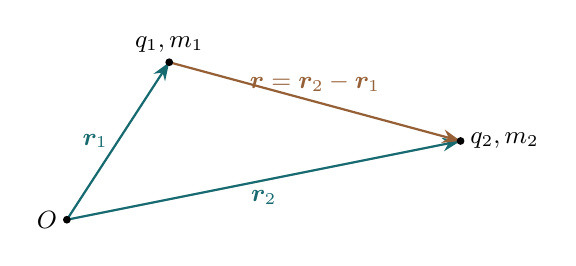
\begin{tikzpicture}[x=1cm,y=1cm]
\coordinate (O) at (0,0);\coordinate (A) at (1.3,2);\coordinate (B) at (5,1);
\draw[motion] (O)--(A) node[midway,left] {$\vect r_1$};\draw[motion] (O)--(B) node[midway,below] {$\vect r_2$};
\draw[force] (A)--(B) node[midway,above] {$\vect r=\vect r_2-\vect r_1$};
\foreach \p in {A,B,O}\fill (\p) circle (1.4pt);
\node[left] at (O) {$O$};\node[above] at (A) {$q_1,m_1$};\node[right] at (B) {$q_2,m_2$};
\end{tikzpicture}\figcaption{图 电1.1　相对位矢从电荷1指向电荷2。}\end{minipage}\end{center}

\Needspace{6\baselineskip}\subsection*{解答}

记$k=1/(4\pi\varepsilon_0)$，$r=|\vect r|$。题图中$\vect r$从电荷1指向电荷2，因而两条运动方程为
\[m_1\ddot{\vect r}_1=-\frac{kq_1q_2}{r^3}\vect r,\qquad
m_2\ddot{\vect r}_2=\frac{kq_1q_2}{r^3}\vect r.\]
第二式除以$m_2$，第一式除以$m_1$，再相减，得
\[\ddot{\vect r}=kq_1q_2\left(\frac1{m_1}+\frac1{m_2}\right)\frac{\vect r}{r^3}.\]
定义约化质量$\mu=m_1m_2/(m_1+m_2)$，相对运动方程便是
\result{\mu\ddot{\vect r}=\frac{kq_1q_2}{r^3}\vect r.}
这条矢量方程适用于任意初始速度；只有第二问给定的静止初态才保证两电荷此后沿初始连线运动。把两条运动方程相加还可得质心加速度为零；本题初始总动量为零，质心始终静止。
\begin{center}\begin{minipage}{0.97\linewidth}\centering
\begin{tikzpicture}[x=1cm,y=1cm]
\draw[guide] (-.5,0)--(6,0);\fill (0,0) circle (2pt) node[above] {$q_1$};\fill (5,0) circle (2pt) node[above] {$q_2$};
\fill (3,0) circle (1.5pt) node[above=5pt] {$C$};
\draw[force] (0,0)--(1.4,0) node[midway,below] {$\vect F_1$};\draw[force] (5,0)--(3.6,0) node[midway,below] {$\vect F_2$};
\draw[<->] (0,.85)--(5,.85) node[midway,above] {$r(t)$};
\node[below=22pt] at (3,0) {质心$C$静止，$\dot r<0$};
\end{tikzpicture}\figcaption{解图 电1.1A　异号电荷相向运动；质心将间距按质量反比分配。}\end{minipage}\end{center}
令$K=k|q_1q_2|>0$。在解图电1.1A所示的相向运动中，标量距离满足
\[\mu\ddot r=-\frac K{r^2},\qquad r(0)=r_0,\qquad\dot r(0)=0.\]
用$\ddot r=\dot r\,\dd\dot r/\dd r$积分，或直接写能量守恒，均得到
\[\frac12\mu\dot r^2-\frac K r=-\frac K{r_0},\qquad
\dot r=-\sqrt{\frac{2K}{\mu}\left(\frac1r-\frac1{r_0}\right)}.\]
负根对应距离随时间减小。把时间写成从当前间距$r$积到初始间距$r_0$，积分值为正：
\[t(r)=\sqrt{\frac{\mu}{2K}}\int_r^{r_0}\sqrt{\frac{r_0s}{r_0-s}}\,\dd s.\]
令$s=r_0\cos^2\theta$，则$\dd s=-2r_0\sin\theta\cos\theta\,\dd\theta$，而$r$对应
$\theta_r=\arccos\sqrt{r/r_0}$。于是
\begin{align*}
t(r)&=2\sqrt{\frac{\mu r_0^3}{2K}}\int_0^{\theta_r}\cos^2\theta\,\dd\theta\\
&=\sqrt{\frac{\mu r_0^3}{2K}}\left[\arccos\sqrt{\frac r{r_0}}+
\sqrt{\frac r{r_0}\left(1-\frac r{r_0}\right)}\right].
\end{align*}
取$r\to0$，得到相碰时间
\result{t_c=\frac\pi2\sqrt{\frac{\mu r_0^3}{2k|q_1q_2|}}
=\pi\sqrt{\frac{\pi\varepsilon_0\mu r_0^3}{2|q_1q_2|}}.}
在 $r=r_0$ 时，时间函数从零开始。由 $t_c\propto r_0^{3/2}$，初始间距加倍使相碰时间乘 $2^{3/2}$。若$m_2\to\infty$，$\mu\to m_1$，还原为电荷1向固定电荷2落下的情形。理想点电荷模型在$r=0$处速度发散，但上述时间积分收敛；这里的相碰时间指该理想模型达到零间距的极限。
\subsubsection*{质心、相对坐标和一维运动的条件}
令$M=m_1+m_2$，质心位置为
$\vect R_C=(m_1\vect r_1+m_2\vect r_2)/M$。
由两式相加得$M\ddot{\vect R}_C=0$，结合相对位矢可反解各自坐标：
\[
\vect r_1=\vect R_C-\frac{m_2}M\vect r,\qquad
\vect r_2=\vect R_C+\frac{m_1}M\vect r.
\]
因此解图电1.1A的C点把两电荷距离按质量反比分配，
静止释放时，两电荷在初始质心相碰。按图中从 $q_1$ 到 $q_2$ 的距离量取，质心位置为 $m_2r_0/M$，等质量时为 $r_0/2$。
相对运动的动量矩$\vect L=\mu\vect r\times\dot{\vect r}$守恒，
因为库仑力沿相对位矢、对相对原点的力矩为零。
本题静止初态给$\vect L=0$，结合中心力才保证连线方向固定，
从而可把矢量方程化为距离r的标量方程。
有非零相对角动量时还要联立极角变化，径向方程会出现角动量项。

动能分解也说明约化质量为何进入能量式：
\[
\frac12m_1|\dot{\vect r}_1|^2+\frac12m_2|\dot{\vect r}_2|^2
=\frac12M|\dot{\vect R}_C|^2+\frac12\mu|\dot{\vect r}|^2.
\]
初始两者均静止时第一项为零，所以相对能量就是全体系动能与相互作用势能之和。
若两者共同匀速平移，第一项为不变常数，相对运动与相碰时间仍相同。

\subsubsection*{用无量纲平方根换元完整复算时间积分}
对前面的时间积分另令$u=\sqrt{s/r_0}$，
有$s=r_0u^2$、$\dd s=2r_0u\dd u$，当前间距对应$u_r=\sqrt{r/r_0}$。
逐项代换得
\[
\begin{aligned}
t(r)&=\sqrt{\frac\mu{2K}}\int_r^{r_0}\sqrt{\frac{r_0s}{r_0-s}}\dd s\\
&=2\sqrt{\frac{\mu r_0^3}{2K}}\int_{u_r}^{1}\frac{u^2}{\sqrt{1-u^2}}\dd u.
\end{aligned}
\]
其中
\[
\int\frac{u^2}{\sqrt{1-u^2}}\dd u
=\frac12\left[\arcsin u-u\sqrt{1-u^2}\right]+C.
\]
代入上下限，令$\tau=\sqrt{\mu r_0^3/(2K)}$，便得
\[
t(r)=\tau\left[\frac\pi2-\arcsin\sqrt{\frac r{r_0}}
+\sqrt{\frac r{r_0}\left(1-\frac r{r_0}\right)}\right].
\]
利用$\pi/2-\arcsin u=\arccos u$，与三角换元结果完全相同。
靠近过程中 $\dot r<0$，用 $\dd t=\dd r/\dot r$ 换为从 $r$ 到 $r_0$ 的正向积分。起点 $r=r_0$ 时积分为零，靠近时积分区间随 $r$ 减小而增大。

\begin{center}\begin{minipage}{.97\linewidth}\centering
\begin{tikzpicture}[x=4.5cm,y=2.8cm,font=\small]
\draw[axis] (0,0)--(1.25,0) node[right] {$t/t_c$};
\draw[axis] (0,0)--(0,1.35) node[above] {$r/r_0$};
\draw[traj,domain=0:90,samples=130,variable=\t]
plot ({\t/90+sin(2*\t)/pi},{cos(\t)*cos(\t)});
\draw[guide] (.818309886,.5)--(0,.5) node[left] {$1/2$};
\draw[guide] (.818309886,0)--(.818309886,.5);
\node[below] at (1,0) {$1$};\node[left] at (0,1) {$1$};
\node at (.65,1.18) {$t_{1/2}/t_c=1/2+1/\pi$};
\end{tikzpicture}
\figcaption{解图 电1.1B　靠近速度逐渐增加，走完前一半间距占总时间约81.8\%。}
\end{minipage}\end{center}
解图电1.1B的初始切线水平，表示由静止释放；接近相碰时曲线越来越陡，
对应相对速率增长。靠近零间距时$|\dot r|\sim\sqrt{2K/(\mu r)}$，
故剩余时间积分按$\int_0^r\sqrt{s}\dd s$收敛，
约为$(2/3)\sqrt{\mu/(2K)}r^{3/2}$。
这段剩余时间按 $r^{3/2}$ 缩小，零间距在有限时刻达到。
若初始有非零相对角动量，径向有效势包含$L^2/(2\mu r^2)-K/r$，
零间距附近，正角动量项主导并使有效势趋于正无穷；有限能量的轨迹转向于正半径。


\Needspace{18\baselineskip}

\pdfbookmark[2]{第 2 题 正方形中心电荷的小振动}{q2}

\section*{第 2 题\quad 正方形中心电荷的小振动}\label{q:2}

边长为$a$的正方形四个顶点各固定一个电量为$Q$的点电荷。中心放一个质量为$m$、电量为$q$的自由点电荷，$qQ>0$。将它沿一条对角线移动很小的距离后由静止释放。判断它是否作周期性振动；若是，求小振动周期，并说明稳定性的空间范围。

\begin{center}\begin{minipage}{0.97\linewidth}\centering
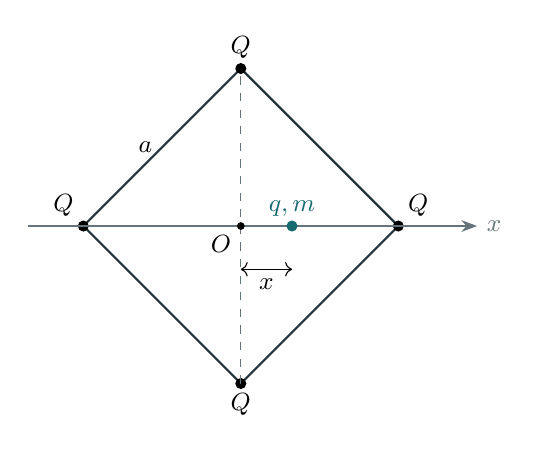
\begin{tikzpicture}[x=1cm,y=1cm]
\draw[object] (-2,0)--(0,2)--(2,0)--(0,-2)--cycle;
\foreach \x/\y in {-2/0,0/2,2/0,0/-2}\fill (\x,\y) circle (2pt);\node[above left] at (-2,0) {$Q$};\node[above] at (0,2) {$Q$};\node[above right] at (2,0) {$Q$};\node[below] at (0,-2) {$Q$};
\draw[axis] (-2.7,0)--(3,0) node[right] {$x$};\draw[guide] (0,-2)--(0,2);
\fill (0,0) circle (1.4pt) node[below left] {$O$};\fill[accent] (.65,0) circle (2pt) node[above] {$q,m$};
\node[left] at (-1,1) {$a$};\draw[<->] (0,-.55)--(.65,-.55) node[midway,below] {$x$};
\end{tikzpicture}\figcaption{图 电1.2　沿水平对角线释放电荷，四个顶点电荷固定。}\end{minipage}\end{center}

\Needspace{6\baselineskip}\subsection*{解答}

记正方形半对角线长$b=a/\sqrt2$，取所移对角线为$x$轴。电荷$q$位于$(x,0)$，$|x|\ll b$。对角线上的两个固定电荷位于$(\pm b,0)$；另一对位于$(0,\pm b)$。以下令$k=1/(4\pi\varepsilon_0)$。
\begin{center}\begin{minipage}{0.97\linewidth}\centering
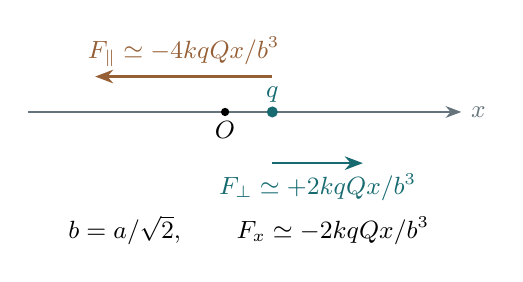
\begin{tikzpicture}[x=1cm,y=1cm]
\draw[axis] (-2.5,0)--(3,0) node[right] {$x$};\fill (0,0) circle (1.5pt) node[below] {$O$};
\fill[accent] (.6,0) circle (2pt) node[above] {$q$};
\draw[force] (.6,.45)--(-1.65,.45) node[midway,above] {$F_{\parallel}\simeq-4kqQx/b^3$};
\draw[motion] (.6,-.65)--(1.75,-.65) node[midway,below] {$F_{\perp}\simeq+2kqQx/b^3$};
\node at (.3,-1.5) {$b=a/\sqrt2,\qquad F_x\simeq-2kqQx/b^3$};
\end{tikzpicture}\figcaption{解图 电1.2A　两组顶点电荷的水平合力方向相反，左向回复项较大。}\end{minipage}\end{center}
解图电1.2A把两组顶点电荷的轴向合力分别画出：沿运动对角线的一组给向左的$-4kqQx/b^3$，垂直对角线的一组给向右的$+2kqQx/b^3$。按同一轴向相加，左向项有一半被右向项抵消，余下的回复系数决定振动频率。

沿$x$轴的一对电荷产生的合力为
\begin{align*}
F_{\parallel}&=kqQ\left[\frac1{(b+x)^2}-\frac1{(b-x)^2}\right]\\
&=\frac{kqQ}{b^2}\left[\left(1+\frac xb\right)^{-2}-\left(1-\frac xb\right)^{-2}\right]
=-\frac{4kqQ}{b^3}x+O(x^3).
\end{align*}
上、下两个电荷的竖直分量相互抵消。每个电荷到$q$的距离为$\sqrt{b^2+x^2}$，其水平投影因子为$x/\sqrt{b^2+x^2}$，所以
\[F_{\perp}=\frac{2kqQx}{(b^2+x^2)^{3/2}}
=\frac{2kqQ}{b^3}x+O(x^3).\]
两组相加，得到小位移下的运动方程
\[m\ddot x=-\frac{2kqQ}{b^3}x,\qquad
\omega^2=\frac{2kqQ}{mb^3}=\frac{\sqrt2\,qQ}{\pi\varepsilon_0ma^3}.\]
因为$qQ>0$，线性项为回复力。沿对角线静止释放时，由对称性运动始终保持在该直线上，小振动近似为简谐运动，其周期为
\result{T=2\pi\sqrt{\frac{mb^3}{2kqQ}}
=\pi\sqrt{\frac{2\sqrt2\,\pi\varepsilon_0ma^3}{qQ}}.}
这个周期是振幅趋于零时的极限；有限振幅的首个修正在后文由完整势能求出。

沿面外法线作位移时，回复力的符号随方向改变。利用正方形的旋转对称性，平面内任意方向的一阶合力均为$-2kqQ\vect r_{\parallel}/b^3$，故平面内稳定。若使电荷向垂直平面的$z$方向移动，则四个电荷的$z$分量同向：
\[F_z=\frac{4kqQz}{(b^2+z^2)^{3/2}}\simeq\frac{4kqQ}{b^3}z.\]
法向力沿位移方向，故法向微扰增长。题设沿严格对角线静止释放时，对称性保持这一条轨迹。
\subsubsection*{势能鞍点与平面内的线性各向同性}
设一般小位移为 $(x,y,z)$，记其长度为 $s$。四个固定电荷到中心的距离都是 $b$。固定电荷关于中心成对布置，势能展开中的奇次项相消，因此
\[
U(x,y,z)=\frac{4kqQ}{b}
+\frac{kqQ}{b^3}(x^2+y^2-2z^2)
+O\left(\frac{k|qQ|}{b}\left(\frac{s}{b}\right)^4\right).
\]
因此势能在x、y方向曲率相同且为正，z方向曲率为负，
Hessian矩阵为$[2kqQ/b^3]\operatorname{diag}(1,1,-2)$。
三个曲率之和为零，与中心附近没有固定电荷的拉普拉斯方程相容。
平面内任意小位移的一阶恢复力相同，
法向曲率为负，中心在三维势能面上为鞍点。

\begin{center}\begin{minipage}{.97\linewidth}\centering
\begin{tikzpicture}[x=6cm,y=5cm,font=\small]
\draw[axis] (-.43,0)--(.48,0) node[right] {$\xi=x/b\text{或}z/b$};
\draw[axis] (0,-.32)--(0,.34) node[above] {$\Delta U/(kqQ/b)$};
\draw[traj,domain=-.35:.35,samples=120] plot(\x,{1/(1-\x)+1/(1+\x)+2/sqrt(1+\x*\x)-4});
\draw[brown,thick,dashed,domain=-.35:.35,samples=120] plot(\x,{4/sqrt(1+\x*\x)-4});
\node at (.23,.25) {沿对角线};\node at (.23,-.29) {沿面外法线};
\node[left] at (0,.2) {$0.2$};\node[left] at (0,-.2) {$-0.2$};
\end{tikzpicture}
\figcaption{解图 电1.2B　同一归一位移下，沿对角线为势阱，沿面外法线为势垒顶部。}
\end{minipage}\end{center}
解图电1.2B两曲线对应同一套四顶点电荷，
实线沿给定对角线取$U(x,0,0)$，虚线沿垂直轴取$U(0,0,z)$。
它们在原点都斜率为零，但曲率相反，于是沿对角线的力指向原点，沿法线的力指向远离原点。
在小振动近似中平面内x、y具有同一频率，
严格沿对角线由静止释放时，对称性还保证横向坐标一直为零。
平面内的高阶势能项依赖方向，所以一般方向的有限振幅轨迹还包含横向偏转。

\subsubsection*{有限振幅的首个周期修正}
沿题设对角线，在$|x|<b$范围完整势能为
\[
U(x)=kqQ\left[\frac1{b-x}+\frac1{b+x}+\frac2{\sqrt{b^2+x^2}}\right].
\]
继续保留四阶项，
\[
U(x)=\frac{4kqQ}b+\frac{kqQ}{b^3}x^2
+\frac{11kqQ}{4b^5}x^4+O(x^6),
\quad F_x=-\frac{2kqQ}{b^3}x-\frac{11kqQ}{b^5}x^3+O(x^5).
\]
三次回复项为负，表明这条方向上的回复力随振幅增强。
若从振幅A静止释放，能量差可写成
\[
\frac12m\dot x^2=\frac{kqQ}{b^3}(A^2-x^2)
\left[1+\frac{11}{4b^2}(A^2+x^2)+O(A^4/b^4)\right].
\]
令$x=A\sin\phi$代入四分之一周期积分，按$A/b$展开，得到
\[
\frac{T(A)}{T_0}
=\frac2\pi\int_0^{\pi/2}\left[1+\frac{11A^2}{4b^2}(1+\sin^2\phi)\right]^{-1/2}\dd\phi
+O(A^4/b^4)
=1-\frac{33}{16}\frac{A^2}{b^2}+O(A^4/b^4).
\]
这里$T_0$为前面求得的小振动周期。
在 $A\ll b$ 的范围内，周期比零振幅极限略短。若释放点接近顶点，应用前面的完整势能积分。


\Needspace{18\baselineskip}

\pdfbookmark[2]{第 3 题 共线四点电荷作用下的轴向运动}{q3}

\section*{第 3 题\quad 共线四点电荷作用下的轴向运动}\label{q:3}

在$x$轴的$x=\pm a$处各固定一个电量为$Q$的点电荷，在$x=\pm2a$处各固定一个电量为$-8Q$的点电荷，$Q>0$。电量为$q>0$、质量为$m$的质点只能沿$x$轴运动。判断原点$O$是否为稳定平衡位置。若稳定，将质点移至$x=A$处静止释放，$0<A\ll a$，求振动周期的主阶表达式。

\begin{center}\begin{minipage}{0.97\linewidth}\centering
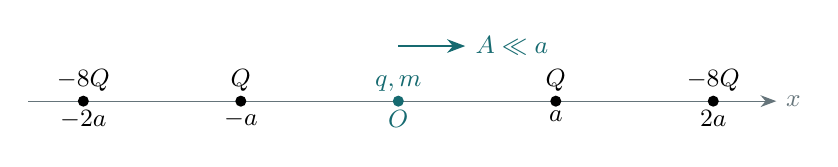
\begin{tikzpicture}[x=1cm,y=1cm]
\draw[axis] (-4.7,0)--(4.8,0) node[right] {$x$};
\foreach \x/\t/\p in {-4/{-8Q}/{-2a},-2/Q/{-a},2/Q/a,4/{-8Q}/{2a}}{\fill (\x,0) circle (2pt);\node[above] at (\x,0) {$\t$};\node[below] at (\x,0) {$\p$};}
\fill[accent] (0,0) circle (2pt) node[above] {$q,m$} node[below] {$O$};
\draw[motion] (0,.7)--(.85,.7) node[right] {$A\ll a$};
\end{tikzpicture}\figcaption{图 电1.3　四个固定电荷共线排列，活动电荷限制在该直线上运动。}\end{minipage}\end{center}

\Needspace{6\baselineskip}\subsection*{解答}

先写$|x|<a$内的有符号合力。两侧$Q$排斥$q$，两侧$-8Q$吸引$q$，所以
\[F_x=kqQ\left[\frac1{(a+x)^2}-\frac1{(a-x)^2}
-\frac8{(2a+x)^2}+\frac8{(2a-x)^2}\right].\]
用$u=x/a$展开，保留到三次项：
\begin{align*}
\frac{a^2F_x}{kqQ}
&=(1+u)^{-2}-(1-u)^{-2}
-2(1+u/2)^{-2}+2(1-u/2)^{-2}\\
&=(-4u-8u^3)+\left(4u+2u^3\right)+O(u^5)\\
&=-6u^3+O(u^5).
\end{align*}
一次项恰好抵消，但三次项未消失。因此
\[F_x\simeq-\beta x^3,\qquad \beta=\frac{6kqQ}{a^5}=\frac{3qQ}{2\pi\varepsilon_0a^5}>0.\]
两个对称电荷对的准确合力还可写成 $4akqQx[16/(4a^2-x^2)^2-1/(a^2-x^2)^2]$。在 $0<|x|<a$ 时，$4(a^2-x^2)<4a^2-x^2$，因此方括号为负，回复力的方向与位移相反。原点的一阶斜率为零，最低阶的回复项为上面得到的三次项。
\begin{center}\begin{minipage}{0.97\linewidth}\centering
\begin{tikzpicture}[x=2.4cm,y=2cm,font=\small]
\draw[axis] (-1.4,0)--(1.55,0) node[right] {$\xi=x/A$};
\draw[axis] (0,-.1)--(0,1.75) node[above] {$U/(\beta A^4/4)$};
\draw[traj,domain=-1.1:1.1,samples=120] plot(\x,{pow(\x,4)});
\draw[guide] (-1,1)--(1,1);\draw[guide] (-1,0) node[below] {$-1$}--(-1,1);
\draw[guide] (1,0) node[below] {$1$}--(1,1);\node[left] at (0,1) {$1$};
\node at (-.75,1.6) {$U/E=\xi^4$};\draw[force] (.65,.15)--(.25,.15);
\end{tikzpicture}\figcaption{解图 电1.3A　原点是四次势阱底部；能量线在两个转折点截出往复范围。}\end{minipage}\end{center}
解图电1.3A画出原点附近的平坦势阱，转折点的高度决定运动能量。取$U(0)=0$，在三次回复力近似下
\[U(x)=-\int_0^xF_x(s)\,\dd s=\frac\beta4x^4.\]
从$x=A$静止释放后，能量守恒给出
\[\frac12m\dot x^2+\frac\beta4x^4=\frac\beta4A^4,
\qquad |\dot x|=\sqrt{\frac\beta{2m}(A^4-x^4)}.\]
图中从$A$运动到$0$恰为四分之一周期，因此
\[T=4\sqrt{\frac{2m}{\beta}}\int_0^A\frac{\dd x}{\sqrt{A^4-x^4}}
=\frac4A\sqrt{\frac{2m}{\beta}}\int_0^1\frac{\dd u}{\sqrt{1-u^4}}.\]
这是有限的反常积分。若用第一类完全椭圆积分
\[\mathsf K(\kappa)=\int_0^{\pi/2}\frac{\dd\phi}{\sqrt{1-\kappa^2\sin^2\phi}},\]
令$u=\cos\phi$，则
\[\int_0^1\frac{\dd u}{\sqrt{1-u^4}}
=\int_0^{\pi/2}\frac{\dd\phi}{\sqrt{1+\cos^2\phi}}
=\frac1{\sqrt2}\mathsf K(1/\sqrt2).\]
由$\mathsf K(1/\sqrt2)\approx1.854074677$得到
\result{T\simeq\frac4A\sqrt{\frac m\beta}\,\mathsf K(1/\sqrt2)
\approx\frac{7.41630}{A}\sqrt{\frac{2\pi\varepsilon_0ma^5}{3qQ}}.}
$A\ll a$保证被略去的五次力项相对三次项为$O(A^2/a^2)$，上式是周期的主阶近似。随振幅减小，周期按 $A^{-1}$ 增大，频率趋零。三次回复力使往复运动呈非简谐。
\subsubsection*{四次势能下的稳定平衡与任意位置的到达时间}
解图电1.3A中最低非零势能项为正的$\beta x^4/4$。
从任意充分小振幅A静止释放，总能量为$\beta A^4/4$，
能量守恒使$|x|\le A$，所以小扰动不会使质点远离原点。
正的四次势能项使有限小能量的运动始终局限在原点附近，故原点为稳定平衡。
在$A=0$时，质点保持静止；
$T\to\infty$描述的是一族非零振幅轨道的极限。

还可保留第一类不完全椭圆积分，描述从A到任意x的运动。
定义
\[
\mathsf F(\Phi,\kappa)=\int_0^\Phi
\frac{\dd\phi}{\sqrt{1-\kappa^2\sin^2\phi}},\qquad
\mathsf K(\kappa)=\mathsf F(\pi/2,\kappa).
\]
对$0\le x\le A$，令$s=A\cos\phi$，两因子分开后有
\[
\begin{aligned}
\int_x^A\frac{\dd s}{\sqrt{(A^2+s^2)(A^2-s^2)}}
&=\int_0^{\arccos(x/A)}\frac{\dd\phi}{\sqrt{A^2+A^2\cos^2\phi}}\\
&=\frac1{\sqrt2A}\mathsf F\left(\arccos\frac xA,\frac1{\sqrt2}\right).
\end{aligned}
\]
因此第一段从A向原点运动的时间为
\[
t(x)=\frac1A\sqrt{\frac m\beta}
\mathsf F\left(\arccos\frac xA,\frac1{\sqrt2}\right).
\]
取$x=0$得$T/4$，再用奇偶对称延续到其余三段，恢复完整周期。
从A到0的时间乘4才给完整周期；其余位置的到达时间则保留不完全积分的上限。
定义中$\kappa$是模数；若计算工具使用参数$\kappa^2$，此处应输入$1/2$。

\subsubsection*{振幅缩放、平均能量与被略去项}
令$y=x/A$，$\tau=A\sqrt{\beta/m}\,t$，
三次回复方程化为
\[
\frac{\dd^2y}{\dd\tau^2}+y^3=0,\qquad
y(0)=1,\quad y'(0)=0.
\]
归一运动与A无关，故物理时间尺度必与$A^{-1}$成正比，
最大速度与$A^2$成正比，最大加速度与$A^3$成正比。
四次势能使回复力按位移三次方变化，因此振幅改变时频率也随之改变。

若需要平均动能，用周期平均的
$\langle\dd(xm\dot x)/\dd t\rangle=0$，
得$2\langle E_k\rangle=4\langle U\rangle$，
所以$\langle E_k\rangle=2E/3$、$\langle U\rangle=E/3$。
四次势阱中，平均动能为平均势能的两倍。

完整电场继续展开给
\[
F_x=-\frac{6kqQ}{a^5}x^3
-\frac{45kqQ}{4a^7}x^5+O(x^7).
\]
在$|x|\le A$上，五次项相对三次项不超过主阶的$(15/8)A^2/a^2$。
这给忽略高次力的具体尺度，周期的主阶误差仍为$O(A^2/a^2)$。
若远处电荷略偏离$-8Q$而恢复一次项，
在足够小的振幅下运动又会由线性项主导；线性项和三次项的相对大小同时取决于参数偏差和振幅。


\Needspace{18\baselineskip}

\pdfbookmark[2]{第 4 题 反平方律与带电球壳的内场}{q4}

\section*{第 4 题\quad 反平方律与带电球壳的内场}\label{q:4}

证明：若真空中的电力严格服从反平方律，一个孤立带电导体球壳达到静电平衡时，电荷均匀分布在外表面，球壳内部电场处处为零。球形空腔内没有电荷，外部没有其他电荷或外加电场。说明证明中反平方律起什么作用。

\begin{center}\begin{minipage}{0.97\linewidth}\centering
\begin{tikzpicture}[x=1cm,y=1cm]
\fill[accent!10] (0,0) circle (1.9);\fill[white] (0,0) circle (1.45);\draw[object] (0,0) circle (1.9);\draw[object] (0,0) circle (1.45);
\fill (0,0) circle (1pt) node[below] {$O$};\fill (.55,.5) circle (1.5pt) node[above] {$P$};
\foreach \t in {0,45,...,315}\node at (\t:2.08) {$+$};
\node[right,align=left] at (2.8,.35) {球形空腔内无电荷\\外部无其他电荷};
\end{tikzpicture}\figcaption{图 电1.4　孤立导体球壳的静电平衡；图示取总电荷为正。}\end{minipage}\end{center}

\Needspace{6\baselineskip}\subsection*{解答}

先在已知均匀带电的球面上计算内场。再用所得零场构造导体的等势状态，最后说明这种分布的唯一性。
\begin{center}\begin{minipage}{0.97\linewidth}\centering
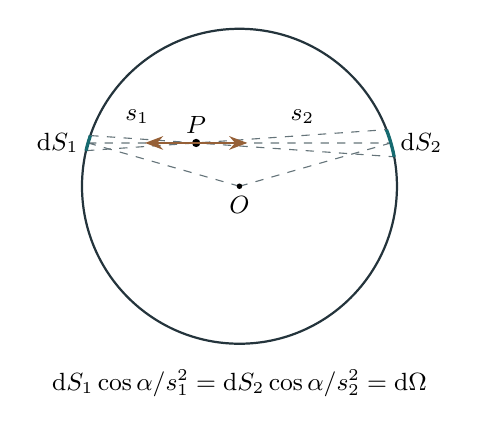
\begin{tikzpicture}[x=1cm,y=1cm,font=\small]
\draw[object] (0,0) circle(2);
\coordinate (O) at (0,0);\coordinate (P) at (-.55,.55);
\coordinate (A) at (-1.922888452303,0.550000000000);\coordinate (B) at (1.922888452303,0.550000000000);

\draw[guide] (A)--(B) (O)--(A) (O)--(B);
\draw[guide] (-1.893497532617,0.643946499310)--(1.964690175953,0.374155732970);
\draw[guide] (-1.948201642550,0.452228216682)--(1.866303874830,0.718964426654);
\draw[very thick,accent] (161.217699286521:2) arc[start angle=161.217699286521,end angle=166.931599616959,radius=2];
\draw[very thick,accent] (10.782300713479:2) arc[start angle=10.782300713479,end angle=21.068400383041,radius=2];

\fill (O) circle(1pt) node[below] {$O$};\fill (P) circle(1.5pt) node[above] {$P$};
\node[left] at (A) {$\dd S_1$};\node[right] at (B) {$\dd S_2$};
\node[above] at (-1.3,.67) {$s_1$};\node[above] at (.8,.67) {$s_2$};
\draw[force] (P)--(.1,.55);\draw[force] (P)--(-1.2,.55);
\node at (0,-2.5) {$\dd S_1\cos\alpha/s_1^2=\dd S_2\cos\alpha/s_2^2=\dd\Omega$};
\end{tikzpicture}\figcaption{解图 电1.4A　同一细双锥两端的面元对P张相同立体角；近面元小、远面元大。}\end{minipage}\end{center}
先考虑半径为$R$、表面电荷密度为常量$\sigma$的薄球面。在内部任取一点$P$；在解图电1.4A中，通过$P$取一个很细的双锥，两端截得面元$\dd S_1,\dd S_2$，到$P$的距离分别为$s_1,s_2$。过球心$O$向这条弦作垂线，垂足把弦平分。两端点与$O$、垂足组成全等直角三角形，所以两端球面法线与弦的锐角相同，记为$\alpha$。两个面元对$P$张相同的立体角，故
\[\dd\Omega=\frac{\dd S_1\cos\alpha}{s_1^2}
=\frac{\dd S_2\cos\alpha}{s_2^2},\qquad
\frac{\dd S_1}{s_1^2}=\frac{\dd S_2}{s_2^2}.\]
依据反平方律，两面元在$P$的场强大小分别为
\[\dd E_1=k|\sigma|\frac{\dd S_1}{s_1^2},\qquad
\dd E_2=k|\sigma|\frac{\dd S_2}{s_2^2}.\]
它们大小相等、方向相反，逐对抵消。让细双锥遍历半个立体角空间，恰好将球面配对一次，因此
\result{\vect E(P)=0\qquad (|OP|<R).}
对任意内部点都可作这样的细双锥；球心处也可直接按对径点配对。

\Needspace{10\baselineskip}
现在回到总电荷为$Q_{\rm tot}$的孤立导体球壳。把全部电荷均匀放在外表面，令
\[\sigma_{\rm out}=\frac{Q_{\rm tot}}{4\pi R_{\rm out}^2},\qquad
\sigma_{\rm in}=0.\]
刚才的球壳结果表明，这一分布在金属内部和空腔内部都给出零电场；外表面等势，满足静电平衡。它也是唯一的平衡分布：对于给定孤立导体总电荷、无内部电荷且无外加场的边界条件，静电场的唯一性排除了另一个不同分布。也可在确定平衡解唯一后，由旋转对称性说明外表面电荷密度必须处处相同。

反平方律与上述面元的几何比例恰好相配。作为比较，若假设力随$s^{-(2+\delta)}$变化，可引入固定长度$\ell$使比例系数的量纲不变。对预先给定的同一均匀带电球面，两面元的场强差含有因子
\[\dd E_{\rm pair}=\frac{k\sigma\,\dd\Omega}{\cos\alpha}
\left[\left(\frac\ell{s_1}\right)^\delta-\left(\frac\ell{s_2}\right)^\delta\right],\]
其中正方向取从近面元一侧指向远面元一侧，图示按$\sigma>0$说明。$\delta=0$时逐对严格抵消；$\delta\ne0$时一般不再如此。偏心内场因而可用于比较距离指数。这里球面电荷分布预先给定；若电荷还能移动，需按所用的力律及导体条件联立确定其分布。
\subsubsection*{由球面电荷积分求内外两侧的电势}
对半径R的固定均匀带电球面，令$s=|OP|$，取OP为积分极轴。
面元到P距离为$\sqrt{R^2+s^2-2Rs\cos\theta}$，
把纬圈电量$\sigma\,2\pi R^2\sin\theta\dd\theta$逐项代入电势，得
\[
\varphi(s)=2\pi k\sigma R^2\int_{-1}^{1}
\frac{\dd u}{\sqrt{R^2+s^2-2Rsu}}
=\frac{2\pi k\sigma R}{s}[(R+s)-|R-s|].
\]
内点$s<R$时绝对值为$R-s$，所以
\[
\varphi(s)=4\pi k\sigma R=\frac{kQ_{\rm tot}}R;
\qquad s>R\text{时},\quad\varphi(s)=\frac{kQ_{\rm tot}}s.
\]
球心用$s\to0$的极限得到同一内势。
解图电1.4B画出这一连续的内外电势：内侧水平段给零梯度，
外侧按$1/s$下降；表面电势连续但法向场存在面电荷引起的跳变。
上述积分直接采用反平方力对应的库仑电势。球内电势与$s$无关，故其梯度为零，得到均匀球壳的内部电场。

\begin{center}\begin{minipage}{.97\linewidth}\centering
\begin{tikzpicture}[x=2.1cm,y=2cm,font=\small]
\draw[axis] (0,0)--(2.7,0) node[right] {$v=s/R$};
\draw[axis] (0,0)--(0,1.6) node[above] {$\varphi/(kQ_{\rm tot}/R)$};
\draw[traj] (0,1)--(1,1);
\draw[traj,domain=1:2.5,samples=100] plot(\x,{1/\x});
\draw[guide] (1,0) node[below] {$1$}--(1,1);
\node[left] at (0,1) {$1$};\node at (.5,1.3) {内侧常势};\node at (1.9,.85) {外侧$1/v$};
\end{tikzpicture}
\figcaption{解图 电1.4B　均匀球面的库仑电势，图示按总电荷非零归一化。}
\end{minipage}\end{center}

\subsubsection*{导体平衡的唯一性及偏心内场}
固定均匀球面的内场证明与导体电荷为何只能如此分布，是两步不同的问题。
对孤立导体给定总电荷、外界无电荷且无穷远势为零，
设存在两套平衡解，差势w在导体外无电荷区域满足拉普拉斯方程，
金属表面差势为同一常数C。
格林恒等式把$\varepsilon_0\int|\nabla w|^2\dd V$化为导体边界项$C\Delta Q$，
无穷远项消失；两解总电荷相同使$\Delta Q=0$。
因此差场处处为零，排除了第二种外部平衡场。
空腔边界等势、内部无电荷时，也由同样的能量积分或极值原理得腔内常势。
因此，在孤立球对称导体的总电荷给定、外界无电荷的条件下，均匀外表面分布给出唯一的平衡外场。

球心的对径面积和距离各自相等，任意各向同性中央力都在这里成对抵消。要从均匀球面内场区分距离指数，可将测点移到偏心位置。
反平方时任意内点的逐对抵消则更强，
它恰好利用解图电1.4A的面积平方因子与距离平方衰减相配。
偏心内点在反平方律下严格示零，距离指数的偏差则可使其出现非零响应。

对预先固定的均匀球面，若力律改为
$k\,\dd q\,\ell^\delta/s^{2+\delta}$，
在靠近球心的小位移$\vect s$处还可定量展开为
\[
\vect E(\vect s)
=-\frac{kQ_{\rm tot}}{3R^3}\,
\delta\left(\frac\ell R\right)^\delta\vect s
+O\left(\frac{k|Q_{\rm tot}|}{R^2}\left|\frac sR\right|^3\right).
\]
一阶系数可由球面方向平均$\langle n_i n_j\rangle=\delta_{ij}/3$求出。
正电球面在$\delta>0$时给向心场，$\delta<0$时给离心场，
$\delta=0$时则对所有内点严格为零。
这一表达式以固定的均匀球面电荷为前提。对假想力律下可自由移动的导体电荷，须由新的平衡关系求表面分布。


\Needspace{18\baselineskip}

\pdfbookmark[2]{第 5 题 异号半圆环在轴线上的电场}{q5}

\section*{第 5 题\quad 异号半圆环在轴线上的电场}\label{q:5}

半径为$R$的圆环位于$xy$平面，圆心为原点。电荷线密度在$y<0$的半圆上为$+\lambda_0$，在$y>0$的半圆上为$-\lambda_0$，其中$\lambda_0>0$。求垂直于圆环平面、通过圆心的$z$轴上任意一点的电场。

\begin{center}\begin{minipage}{0.97\linewidth}\centering
\begin{tikzpicture}[x=1cm,y=1cm]
\draw[axis] (-2.4,0)--(2.5,0) node[right] {$x$};\draw[axis] (0,-2.2)--(0,2.3) node[above] {$y$};
\draw[very thick,warm] (-1.7,0) arc (180:360:1.7);\draw[very thick,accent] (1.7,0) arc (0:180:1.7);
\node at (0,-1.1) {$+\lambda_0$};\node at (0,1.1) {$-\lambda_0$};\node[below left] at (0,0) {$O$};
\draw[<->] (0,0)--({1.7/sqrt(2)},{-1.7/sqrt(2)}) node[midway,above] {$R$};\node[right,align=left] at (3,.2) {$z$轴垂直纸面\\观察点$P=(0,0,z)$};
\end{tikzpicture}\figcaption{图 电1.5　俯视圆环：下半环带正电，上半环带负电。}\end{minipage}\end{center}

\Needspace{6\baselineskip}\subsection*{解答}

观察点取$P=(0,0,z)$。圆环所在的几何轴是 $z$ 轴。上、下半环线密度异号，沿图中的反射配对决定合场方向。
\begin{center}\begin{minipage}{0.97\linewidth}\centering
\begin{tikzpicture}[x=1cm,y=1cm]
\draw[axis] (-2.6,0)--(2.8,0) node[right] {$y$};\draw[axis] (0,-.3)--(0,3) node[above] {$z$};
\coordinate (P) at (0,1.8);\fill (P) circle (1.5pt) node[left] {$P$};
\fill[warm] (-1.6,0) circle (2pt) node[below] {$+\dd q$};\fill[accent] (1.6,0) circle (2pt) node[below] {$-\dd q$};
\draw[guide] (-1.6,0)--(P)--(1.6,0);\draw[force] (P)--(.8,2.7) node[right] {$\dd\vect E_+$};
\draw[motion] (P)--(.8,.9) node[right] {$\dd\vect E_-$};\draw[very thick,->] (P)--(1.6,1.8) node[right] {$\dd\vect E$};
\node at (0,-.8) {图示一对$x=0$的对称元；一般元再配$x\leftrightarrow-x$};
\end{tikzpicture}\figcaption{解图 电1.5A　正、负电荷的轴向分量抵消，y分量相加；横向分量须另由x对称配对消去。}\end{minipage}\end{center}
先按解图电1.5A配对：关于$x$轴对称的正、负电荷元对$P$等距，电荷大小相等，其$z$分量抵消、$y$分量同向；再用$x\leftrightarrow-x$的对称元消去$x$分量。于是总场只能沿$+y$方向。

取环上位置$\vect r'=(R\cos\phi,R\sin\phi,0)$，$\dd q=\lambda(\phi)R\dd\phi$，所有电荷元到$P$的距离相同：$d=\sqrt{R^2+z^2}$。有
\[\dd\vect E=\frac{k\lambda(\phi)R\dd\phi}{d^3}
(-R\cos\phi,-R\sin\phi,z).\]
其中$0<\phi<\pi$时$\lambda=-\lambda_0$，$\pi<\phi<2\pi$时$\lambda=+\lambda_0$。逐分量积分，
\begin{align*}
E_x&=-\frac{kR^2}{d^3}\int_0^{2\pi}\lambda(\phi)\cos\phi\,\dd\phi=0,\\
E_z&=\frac{kRz}{d^3}\left(-\lambda_0\pi+\lambda_0\pi\right)=0,\\
E_y&=-\frac{kR^2}{d^3}\left[-\lambda_0\int_0^\pi\sin\phi\,\dd\phi
+\lambda_0\int_\pi^{2\pi}\sin\phi\,\dd\phi\right]\\
&=\frac{4k\lambda_0R^2}{(R^2+z^2)^{3/2}}.
\end{align*}
\Needspace{4\baselineskip}
因此，轴上总场为
\result{\vect E(0,0,z)=\frac{\lambda_0R^2}{\pi\varepsilon_0(R^2+z^2)^{3/2}}\vect e_y.}
在$z=0$处，两半圆环各贡献$2k\lambda_0/R$，方向均从带正电的下半环指向带负电的上半环。结果对$z$为偶函数，因此在圆环上下两侧方向相同。

在远处，把圆环看成以偶极矩为首项的分布。总电荷为零，而电偶极矩为
\[\vect p=\int\vect r'\,\dd q=-4\lambda_0R^2\vect e_y.\]
$z$轴是该偶极矩的赤道方向，远处有$\vect E\simeq-k\vect p/|z|^3$，与上式的$|z|\gg R$极限相符。
\subsubsection*{半圆分量的逐次投影与轴上场强曲线}
还可只取正半圆计算，再利用正、负配对把y分量乘2。
在下半圆用$\theta\in[0,\pi]$记从负x端到正x端的角参数，
电荷元位置为$(-R\cos\theta,-R\sin\theta,0)$。
对$z>0$，面元到P的连线与z轴夹角为$\alpha$，有$\sin\alpha=R/d$。
先投影到环面、再投影到y轴，得到
\[
\dd E=\frac{k\lambda_0R\dd\theta}{d^2},\quad
\dd E_{xy}=\dd E\frac Rd,\quad
\dd E_y=\dd E_{xy}\sin\theta
=\frac{k\lambda_0R^2}{d^3}\sin\theta\dd\theta.
\]
因$d=\sqrt{R^2+z^2}$与积分角无关，正半环的贡献为
\[
E_{y,+}=\frac{k\lambda_0R^2}{d^3}\int_0^\pi\sin\theta\dd\theta
=\frac{2k\lambda_0R^2}{d^3},\qquad E_y=2E_{y,+}.
\]
这与前面的有符号矢量积分相同。对$z<0$虽轴向分量反转，
正负两元的轴向分量仍抵消，横向场仍沿$+y$。

\begin{center}\begin{minipage}{.97\linewidth}\centering
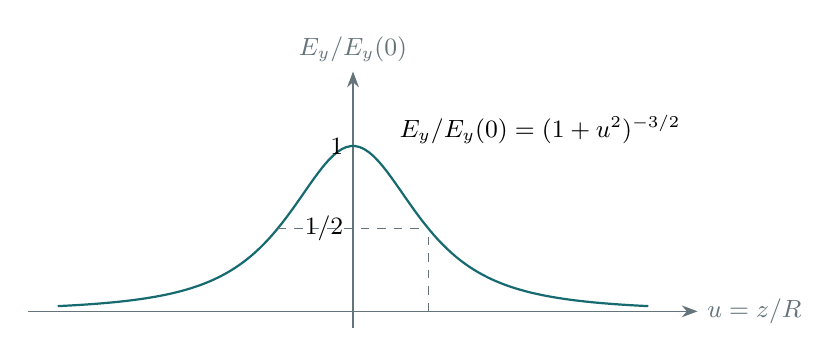
\begin{tikzpicture}[x=1.25cm,y=2.1cm,font=\small]
\draw[axis] (-3.3,0)--(3.5,0) node[right] {$u=z/R$};
\draw[axis] (0,-.1)--(0,1.45) node[above] {$E_y/E_y(0)$};
\draw[traj,domain=-3:3,samples=130] plot(\x,{pow(1+\x*\x,-1.5)});
\draw[guide] (-.76642094,.5)--(.76642094,.5);
\draw[guide] (.76642094,0)--(.76642094,.5);
\node[left] at (0,1) {$1$};\node[left] at (0,.5) {$1/2$};
\node at (1.9,1.1) {$E_y/E_y(0)=(1+u^2)^{-3/2}$};
\end{tikzpicture}
\figcaption{解图 电1.5B　环心场最大；两侧半高位置满足$|z|/R=\sqrt{2^{2/3}-1}$。}
\end{minipage}\end{center}
解图电1.5B的曲线关于 $z=0$ 偶对称，上、下两侧场都沿 $+y$。
近环心有$E_y/E_y(0)=1-3z^2/(2R^2)+O(z^4/R^4)$，
远处则有
\[
\vect E=\frac{4k\lambda_0R^2}{|z|^3}
\left[1-\frac{3R^2}{2z^2}+O(R^4/z^4)\right]\vect e_y.
\]
总电荷为零使单极项消失，前面从偶极矩所得的是首个 $|z|^{-3}$ 项，
更高修正相对它为$O(R^2/z^2)$。

\subsubsection*{零电势轴与非零横向梯度}
轴上所有电荷元等距，所以$\varphi(0,0,z)=k\int\dd q/d=0$。
沿轴求导得到 $E_z=0$，横向的电场由轴旁电势的变化给出。
令$f(z)=4k\lambda_0R^2(R^2+z^2)^{-3/2}$，
在轴旁的小横向位移y处，势的首项为
\[
\varphi(0,y,z)=-f(z)y+O(y^3),\quad
E_y(0,y,z)=f(z)+O(y^2),\quad
E_z(0,y,z)=f'(z)y+O(y^3).
\]
势对y为奇函数，因为$y\to-y$同时交换正负电荷半环。
沿轴取 $y=0$，势恒为零，故沿轴求导得到 $E_z=0$。横向的势梯度由 $-f(z)y$ 给出，在轴上取 $\partial\varphi/\partial y=-f(z)$。轴旁的一阶 $E_z$ 则给 $\partial E_z/\partial y=\partial E_y/\partial z=f'(z)$（取在轴上）。
解图电1.5A中的合场正对应这个横向梯度。


\Needspace{18\baselineskip}

\pdfbookmark[2]{第 6 题 半圆弧与两条半无限直线的电场}{q6}

\section*{第 6 题\quad 半圆弧与两条半无限直线的电场}\label{q:6}

一条均匀带电细线弯成图示形状：左侧$AB$为半圆弧；$AA'$和$BB'$为分别与圆弧相切、向右无限延伸的两条平行直线。求半圆圆心$O$处的电场。可自设圆弧半径$R$和电荷线密度$\lambda$。

\begin{center}\begin{minipage}{0.97\linewidth}\centering
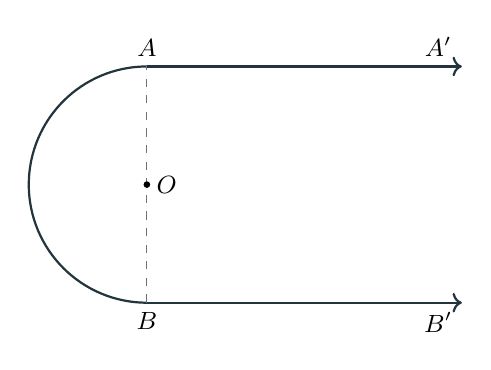
\begin{tikzpicture}[x=1cm,y=1cm]\draw[object] (0,1.5) arc (90:270:1.5);\draw[object,->] (0,1.5)--(4,1.5);\draw[object,->] (0,-1.5)--(4,-1.5);\draw[guide] (0,-1.5)--(0,1.5);\fill (0,0) circle (1.2pt) node[right] {$O$};\node[above] at (0,1.5) {$A$};\node[below] at (0,-1.5) {$B$};\node[above] at (3.7,1.5) {$A'$};\node[below] at (3.7,-1.5) {$B'$};\end{tikzpicture}\figcaption{图 电1.6　两条直线从圆弧端点向右无限延伸，线密度处处相同。}\end{minipage}\end{center}

\Needspace{6\baselineskip}\subsection*{解答}

设$\lambda>0$，最后的矢量结论同样适用于负线密度。解图电1.6A中上、下直线关于水平轴对称，其竖直场分量相消；左半圆弧在$O$的合场向右，两条直线在$O$的合场向左。需要比较两者大小。
\begin{center}\begin{minipage}{0.97\linewidth}\centering
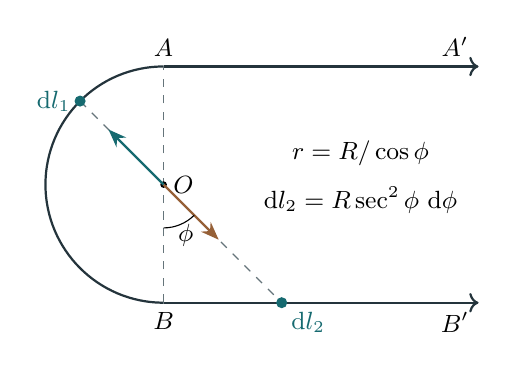
\begin{tikzpicture}[x=1cm,y=1cm]\draw[object] (0,1.5) arc (90:270:1.5);\draw[object,->] (0,1.5)--(4,1.5);\draw[object,->] (0,-1.5)--(4,-1.5);\draw[guide] (0,-1.5)--(0,1.5);\fill (0,0) circle (1.2pt) node[right] {$O$};\node[above] at (0,1.5) {$A$};\node[below] at (0,-1.5) {$B$};\node[above] at (3.7,1.5) {$A'$};\node[below] at (3.7,-1.5) {$B'$};
\draw[guide] ({-1.5/sqrt(2)},{1.5/sqrt(2)})--(1.5,-1.5);\fill[accent] ({-1.5/sqrt(2)},{1.5/sqrt(2)}) circle (2pt) node[left] {$\dd l_1$};\fill[accent] (1.5,-1.5) circle (2pt) node[below right] {$\dd l_2$};
\draw[force] (0,0)--(.7,-.7);\draw[motion] (0,0)--(-.7,.7);
\draw (0,-.55) arc (-90:-45:.55);\node at (.28,-.65) {$\phi$};\node at (2.5,.4) {$r=R/\cos\phi$};\node at (2.5,-.2) {$\dd l_2=R\sec^2\phi\,\dd\phi$};
\end{tikzpicture}\figcaption{解图 电1.6A　左上四分之一弧与下方直线逐元配对；反向场元恰好等大。}\end{minipage}\end{center}
先保留逐元配对法。取左上四分之一弧上一段$\dd l_1$，其到$O$的连线延长后交下方直线于$\dd l_2$。令连线与向下竖直方向夹角为$\phi$，则
\[\dd l_1=R\dd\phi,\qquad r=\frac R{\cos\phi},\qquad
x=R\tan\phi,\qquad \dd l_2=R\sec^2\phi\,\dd\phi.\]
两段电荷产生的电场大小为
\[\dd E_1=\frac{k\lambda\dd l_1}{R^2}=\frac{k\lambda}{R}\dd\phi,\qquad
\dd E_2=\frac{k\lambda\dd l_2}{r^2}=\frac{k\lambda}{R}\dd\phi.\]
两个电荷元位于$O$两侧同一直线上，电场方向相反，所以逐对抵消。当$0\le\phi<\pi/2$时，左上四分之一弧与整个下方半无限直线一一对应；左下四分之一弧同样与上方直线配对。由此得到
\result{\vect E(O)=\vect0.}

也可逐段积分，分别求出三部分的场。左半圆弧的水平场为
\[E_{{\rm arc},x}=-\frac{k\lambda}{R}\int_{\pi/2}^{3\pi/2}\cos\theta\,\dd\theta
=\frac{2k\lambda}{R}.\]
上方直线电荷元$(x,R)$在$O$的场为
\[\dd\vect E_{\rm top}=-k\lambda\frac{x\vect e_x+R\vect e_y}{(x^2+R^2)^{3/2}}\dd x.\]
利用
\[\int_0^\infty\frac{x\dd x}{(x^2+R^2)^{3/2}}=\frac1R,\qquad
\int_0^\infty\frac{R\dd x}{(x^2+R^2)^{3/2}}=\frac1R,\]
得$\vect E_{\rm top}=-(k\lambda/R)(\vect e_x+\vect e_y)$。下方直线给出
$\vect E_{\rm bottom}=-(k\lambda/R)(\vect e_x-\vect e_y)$，三部分相加确为零。

上下对称消去竖直分量；半圆与两条同密度半无限切线的场则在水平方向恰好相消。截短直线后的剩余场见下文。
\subsubsection*{线元投影、无穷端点与配对的适用条件}
解图电1.6A中，将下直线元$\dd l_2$投影到垂直于OP的方向，记投影长度为$\dd l_2'$。
同一小张角给$\dd l_2'=r\dd\phi$，而投影关系给
\[
\dd l_2'=\dd l_2\cos\phi,\qquad
\cos\phi=\frac Rr,\qquad
\frac{\dd l_2}{r^2}=\frac{\dd\phi}{r\cos\phi}=\frac{\dd\phi}R.
\]
这与$x=R\tan\phi$的导数计算是同一几何关系。
同张角下，直线元较长，这个长度因子恰与更大的距离平方相消。
当$\phi\to\pi/2$，对应点$x\to\infty$，
配对应理解为有限角区间逐渐逼近端点的反常积分极限。
单条直线的场积分因被积函数按$x^{-2}$或更快衰减而收敛，
所以取这一极限不会留下额外的端点场。

镜面对称给 $E_y(O)=0$，各段场的水平部分由前面的配对或分段积分得到。

若两条直线都在长度L处截断，水平合场的完整计算为
\[
\begin{aligned}
E_{{\rm lines},x}
&=-2k\lambda\int_0^L\frac{x\dd x}{(x^2+R^2)^{3/2}}\\
&=-2k\lambda\left(\frac1R-\frac1{\sqrt{R^2+L^2}}\right),\\
E_x(O)&=\frac{2k\lambda}{\sqrt{R^2+L^2}}.
\end{aligned}
\]
解图电1.6B按正线密度归一；长度增加时残余场向右且逐渐减小，
按 $2k\lambda/L$ 的尺度减小并在半无限极限趋零。

\begin{center}\begin{minipage}{.97\linewidth}\centering
\begin{tikzpicture}[x=1.6cm,y=2.1cm,font=\small]
\draw[axis] (0,0)--(4.7,0) node[right] {$u=L/R$};
\draw[axis] (0,-.1)--(0,1.4) node[above] {$E_x/(2k\lambda/R)$};
\draw[traj,domain=0:4.3,samples=100] plot(\x,{1/sqrt(1+\x*\x)});
\node[left] at (0,1) {$1$};\node at (2.7,1.05) {$(1+u^2)^{-1/2}$};
\draw[guide] (1,0) node[below] {$1$}--(1,.707106781);
\node[right] at (1,.707106781) {$1/\sqrt2$};
\end{tikzpicture}
\figcaption{解图 电1.6B　两直线截短后的环心残余场；纵轴按$\lambda>0$归一。}
\end{minipage}\end{center}

\subsubsection*{零场点附近是否稳定}
考察离开 $O$ 一小段后的运动，需要求该处电场的一阶变化。
按解图电1.6A，以两条切线的延伸方向为 $+x$、由下切线指向上切线为 $+y$，取 $z$ 垂直于这两条直线和半圆所在的平面，
在O附近对库仑场求一阶导数：每个电荷元贡献
\[
J_{ij}=k\int\frac{\dd q}{r'^3}(\delta_{ij}-3n_i n_j),
\qquad\vect n=\vect r'/r',\quad\vect E(\vect r)=J\vect r+O(|\vect r|^2).
\]
半圆弧给$J_{\rm arc}=(k\lambda/R^2)\operatorname{diag}(-\pi/2,-\pi/2,\pi)$。
两条直线的x导数积分为
$2k\lambda\int_0^\infty(R^2-2x^2)(x^2+R^2)^{-5/2}\dd x=0$，
y、z导数分别为$-2k\lambda/R^2$和$2k\lambda/R^2$，交叉项由对称性消去。
故
\[
J=\frac{k\lambda}{R^2}\operatorname{diag}\left(-\frac\pi2,-\frac\pi2-2,\pi+2\right),
\qquad\operatorname{tr}J=0.
\]
若$\lambda>0$、试探电荷为正且受到平面约束，两个允许方向都有一阶回复力；
若允许三维位移，法向电场随法向偏离同向增长，因而出现失稳。


\Needspace{18\baselineskip}

\pdfbookmark[2]{第 7 题 均匀带电半圆环的圆心电场}{q7}

\section*{第 7 题\quad 均匀带电半圆环的圆心电场}\label{q:7}

半径为$R$的半圆环均匀带电，电荷线密度为$\lambda$。半圆环位于$xy$平面内的$x\le0$一侧，圆心为原点$O$。求圆心处的电场，并给出方向。

\begin{center}\begin{minipage}{0.97\linewidth}\centering
\begin{tikzpicture}[x=1cm,y=1cm]
\draw[axis] (-2.2,0)--(2.3,0) node[right] {$x$};\draw[axis] (0,-2)--(0,2) node[above] {$y$};
\draw[very thick,accent] (0,1.6) arc (90:270:1.6);\draw[guide] (0,0)--(135:1.6) node[midway,below] {$R$};
\node[below right] at (0,0) {$O$};\node[left] at (-1.6,0) {$\lambda$};
\end{tikzpicture}\figcaption{图 电1.7　半圆环位于左半平面；电荷符号由线密度给出。}\end{minipage}\end{center}

\Needspace{6\baselineskip}\subsection*{解答}

对称于$x$轴的两个弧元，在圆心处的$y$分量互相抵消，$x$分量相加。先以$\lambda>0$说明方向：所有弧元的水平分量均向右，所以合场指向半圆的开口。
\begin{center}\begin{minipage}{0.97\linewidth}\centering
\begin{tikzpicture}[x=1cm,y=1cm,font=\small]
\draw[object] (0,1.7) arc(90:270:1.7);
\draw[axis] (-2.2,0)--(2.7,0) node[right] {$x$};
\draw[axis] (0,-1.9)--(0,2.1) node[above] {$y$};
\coordinate (D) at (150:1.7);\draw[guide] (D)--(0,0);
\fill (D) circle(1.5pt) node[above left=5pt] {$\dd l$};
\draw[force] (0,0)--(1.4,{-1.4/sqrt(3)}) node[right] {$\dd\vect E$};
\draw[motion] (0,0)--(1.4,0) node[above] {$\dd E_x$};
\draw[guide] (1.4,0)--(1.4,{-1.4/sqrt(3)});
\draw (.55,0) arc(0:-30:.55);\node at (.76,-.22) {$\alpha$};
\coordinate (D1) at (153:1.7);\coordinate (D2) at (147:1.7);
\draw[very thick,accent] (D1) arc(153:147:1.7);
\draw[guide] (D1)--(D1|-D2)--(D2);
\begin{scope}[shift={(3.4,.1)}]
\draw[object] (0,0)--(.7,1.212435565)--(0,1.212435565)--cycle;
\draw (.175,.303108891) arc(60:90:.35);
\node at (.15,.55) {$\alpha$};
\node[right] at (.45,.65) {$\dd l$};\node[left] at (0,.65) {$\dd y$};
\node at (.35,-.5) {局部放大};
\end{scope}
\node at (.1,-2.3) {$\dd y=\dd l\cos\alpha$};
\end{tikzpicture}\figcaption{解图 电1.7A　将弧元投影到直径上：每个场元的x分量正比于投影长度。}\end{minipage}\end{center}
设一个弧元在$O$的场与$+x$方向夹角为$\alpha$。圆环切线与$y$轴也成相同锐角，解图电1.7A中的直径投影长满足
\[\dd y=\dd l\cos\alpha.\]
因各弧元到圆心的距离都是$R$，其场的水平分量为
\[\dd E_x=\frac{k\lambda\dd l}{R^2}\cos\alpha=\frac{k\lambda}{R^2}\dd y.\]
沿左半圆从下端到上端遍历，$y$从$-R$到$R$且单调变化，投影只覆盖直径一次。因此
\[E_x=\frac{k\lambda}{R^2}\int_{-R}^{R}\dd y=\frac{2k\lambda}{R},\qquad E_y=0.\]
\Needspace{4\baselineskip}
所求圆心场为
\result{\vect E(O)=\frac{\lambda}{2\pi\varepsilon_0R}\vect e_x,
\qquad |\vect E|=\frac{|\lambda|}{2\pi\varepsilon_0R}.}
$\lambda<0$时方向反向，指向左侧带负电的圆弧。

\Needspace{12\baselineskip}
若直接用极角$\theta$，弧元电荷为$\lambda R\dd\theta$，
\[\vect E=-\frac{k\lambda}{R}\int_{\pi/2}^{3\pi/2}
(\cos\theta\vect e_x+\sin\theta\vect e_y)\,\dd\theta
=\frac{2k\lambda}{R}\vect e_x.\]
也可以借助第6题：同密度半圆弧与两条相切半无限直线的场和为零，而两条直线的场为$-2k\lambda\vect e_x/R$，故半圆弧的场应为其相反数。三种方法分别对应直径投影、分量积分和已知结果的叠加。
\subsubsection*{投影的权重与有符号线密度}
解图电1.7A中的$\alpha$同时是场元与x轴、弧元切线与y轴的锐角，
所以$\cos\alpha=\sqrt{R^2-y^2}/R$。
端点附近投影因子趋零，最左端附近则趋近1，等长弧元的水平贡献并不相等。
半圆密度随位置变化时，保留直径参数并在积分内代入该处的密度：
\[
E_x=\frac{k}{R^2}\int_{-R}^{R}\lambda(y)\dd y,\qquad
E_y=-\frac{k}{R^2}\int_{-R}^{R}\frac{\lambda(y)y}{\sqrt{R^2-y^2}}\dd y.
\]
第二式给场元竖直分量的积分。若 $\lambda(y)$ 为偶函数，被积函数关于 $y=0$ 为奇，故 $E_y=0$。两式都在用同一弧元，只是将位置变量换成直径坐标。

对均匀密度，总电量$q=\pi R\lambda$，
各场元大小之和为$k|q|/R^2$，矢量合场大小为其$2/\pi$倍。
若保持q而使R加倍，密度同时减半，场变为四分之一；
若保持$\lambda$，电量随R加倍，场才变为二分之一。
圆心各元电势作代数和，得到 $\pi k\lambda$；电场的水平分量按前面的投影求和。

\subsubsection*{离开环面后的两个分量}
仍取左半圆，在垂直平面的z轴上取P，所有线元到P的距离为$d=\sqrt{R^2+z^2}$。
有符号积分给
\[
\begin{aligned}
\vect E(0,0,z)&=\frac{k\lambda R}{d^3}
\int_{\pi/2}^{3\pi/2}(-R\cos\theta,-R\sin\theta,z)\dd\theta\\
&=\frac{2k\lambda R^2}{d^3}\vect e_x
+\frac{\pi k\lambda Rz}{d^3}\vect e_z.
\end{aligned}
\]
解图电1.7B把两分量按圆心场$E_0=2k\lambda/R$归一。
x分量在两侧同号，z分量随z变号；只有环面上的$z=0$使轴向分量恰好为零。
这与第5题不同：此处半圆总电荷非零，没有另一异号半环消去轴向场。

\begin{center}\begin{minipage}{.97\linewidth}\centering
\begin{tikzpicture}[x=1.2cm,y=1.7cm,font=\small]
\draw[axis] (-3.2,0)--(3.5,0) node[right] {$u=z/R$};
\draw[axis] (0,-.85)--(0,1.35) node[above] {$E_x/E_0,\ E_z/E_0$};
\draw[traj,domain=-3:3,samples=130] plot(\x,{pow(1+\x*\x,-1.5)});
\draw[brown,thick,dashed,domain=-3:3,samples=130] plot(\x,{pi*\x/2*pow(1+\x*\x,-1.5)});
\node[left] at (0,1) {$1$};\node at (-1.9,.9) {实线：x分量};
\node at (2,.8) {虚线：z分量};\node at (1.7,-.65) {$E_0=2k\lambda/R$};
\end{tikzpicture}
\figcaption{解图 电1.7B　均匀半圆的轴上电场分量；$\lambda\ne0$时归一化，零密度时场为零。}
\end{minipage}\end{center}
远处z分量首项为$kq\,\operatorname{sgn}(z)/z^2$，
x分量为$2k\lambda R^2/|z|^3$，分别对应净电荷和横向偶极矩。
沿 $z$ 对 $\varphi(0,0,z)=\pi k\lambda R/d$ 求导可得轴向分量。横向分量对应 $x$ 导数，需要用轴旁的势，或沿用上面的矢量积分。


\Needspace{18\baselineskip}

\pdfbookmark[2]{第 8 题 球形区域内电场的体积平均}{q8}

\section*{第 8 题\quad 球形区域内电场的体积平均}\label{q:8}

固定点电荷$5Q$和$12Q$分别位于$A,B$，$AB=13a$。另一点$C$满足$CA=5a$、$CB=12a$。对以$C$为球心的球形区域，定义电场的体积平均
\[\overline{\vect E}=\frac1V\int_V\vect E\,\dd V.\]
分别求球半径为$a$、$10a$时$|\overline{\vect E}|$。注意所求是电场矢量的平均值的大小。

\begin{center}\begin{minipage}{0.97\linewidth}\centering
\begin{tikzpicture}[x=1cm,y=1cm]
\coordinate (C) at (0,0);\coordinate (A) at (-1.5,0);\coordinate (B) at (0,-3.6);
\draw[object] (A)--(C)--(B)--cycle;\draw (0,-.2)--(-.2,-.2)--(-.2,0);
\node[above left=3pt] at (A) {$A,5Q$};\node[right] at (B) {$B,12Q$};\node[above right] at (C) {$C$};
\node[below=3pt] at (-.75,0) {$5a$};\node[right] at (0,-1.8) {$12a$};\node[left] at (-.8,-1.8) {$13a$};
\draw[guide] (C) circle (.3);\draw[guide] (C) circle (3);\node[right] at (2.6,1.65) {$s=10a$};\node at (.7,-.55) {$s=a$};
\end{tikzpicture}\figcaption{图 电1.8　截面中的直角三角形；大球包含A，小球不含任何电荷。}\end{minipage}\end{center}

\Needspace{6\baselineskip}\subsection*{解答}

由$5^2+12^2=13^2$，$\angle ACB=90^\circ$。建立单位矢量$\vect e_x=\overrightarrow{AC}/(5a)$、$\vect e_y=\overrightarrow{BC}/(12a)$，它们互相垂直。先求一个点电荷在球形区域内的平均电场，再做矢量叠加。
\begin{center}\begin{minipage}{0.97\linewidth}\centering
\begin{tikzpicture}[x=1cm,y=1cm]
\fill[accent!8] (0,0) circle (1.5);\draw[object] (0,0) circle (1.5);\fill (0,0) circle (1.2pt) node[below] {$C$};
\fill (3,0) circle (2pt) node[above] {$q_*$};\draw[motion] (0,0)--(3,0) node[midway,above] {$\vect d$};
\draw[force] (3,-.35)--(4,-.35) node[below] {$\vect F_*$};\draw[force] (0,-.4)--(-1,-.4) node[below] {$Q_t\overline{\vect E}$};
\node at (0,1.9) {辅助均匀球，总电荷$Q_t$};
\begin{scope}[xshift=7cm]\draw[object] (0,0) circle (1.5);\draw[guide] (0,0) circle (.65);\fill (0,0) circle (1.2pt) node[left] {$C$};\fill (.65,0) circle (2pt) node[right] {$q_*$};\draw[motion] (0,0)--(.65,0);\node at (0,1.9) {球内电荷：只计半径$d$内};\end{scope}
\end{tikzpicture}\figcaption{解图 电1.8A　利用作用与反作用，把场的体积平均换成均匀带电球对点电荷的力。}\end{minipage}\end{center}
解图电1.8A中，辅助均匀球与外部点电荷间的两根力箭头相反。均匀球受到的总力是$Q_t\overline{\vect E}$，点电荷受到的力可由球对称场直接求得；以作用与反作用连接两者，才能把体积平均换成已知的球场结果。对球内外的点电荷须分别使用相应球场公式。

设球心为$C$、半径为$s$，点电荷$q_*$的位置相对$C$为$\vect d$，$d=|\vect d|$。在整个球内假想均匀放入总量为$Q_t$的辅助电荷，其体密度为$Q_t/V$。点电荷对辅助球的总作用力为
\[\vect F_t=\int_V\frac{Q_t}{V}\vect E\,\dd V=Q_t\overline{\vect E}.\]
辅助球对点电荷的力$\vect F_*$与之相反。对完整均匀球，在点电荷所在半径$d$处作以$C$为球心的高斯面。
球对称性使场沿径向，同一高斯面上场强大小相同。球外高斯面包围全部$Q_t$，
球内高斯面只包围$Q_t(d/s)^3$，因此分别有
\[
4\pi d^2E_t(d)=\frac{Q_t}{\varepsilon_0}\quad(d>s),\qquad
4\pi d^2E_t(d)=\frac{Q_t d^3}{\varepsilon_0s^3}\quad(d<s).
\]
这里辅助电荷取$Q_t>0$；用径向单位矢量$\vect d/d$恢复方向，得到
\[\vect E_t(\vect d)=
\begin{cases}kQ_t\vect d/d^3,&d>s,\\ kQ_t\vect d/s^3,&d<s.\end{cases}\]
外部结果等效于球心点电荷；内部结果则仅由半径$d$以内电荷$Q_td^3/s^3$产生。由
$Q_t\overline{\vect E}=-q_*\vect E_t$得
\[\overline{\vect E}=
\begin{cases}-kq_*\vect d/d^3,&d>s,\\-kq_*\vect d/s^3,&d<s.\end{cases}\]
因此，外部点电荷的平均场等于它在球心的场；内部点电荷的平均场等于其球心场乘以$(d/s)^3$。此关系连接的是球内场的体积积分与球心处的单个数值。内部点电荷的场在自身位置有奇点，但$|E|\dd V$在其附近按$\dd r$积分，三维体积积分仍然存在。

当$s=a$时，两电荷均在球外：
\[\overline{\vect E}=\frac{kQ}{a^2}\left(\frac15\vect e_x+\frac1{12}\vect e_y\right),\]
故
\result{|\overline{\vect E}|=\frac{k|Q|}{a^2}\sqrt{\frac1{25}+\frac1{144}}
=\frac{13k|Q|}{60a^2}.}
当$s=10a$时，$A$在球内而$B$在球外。$A$的贡献须乘以$(5/10)^3=1/8$，所以
\[\overline{\vect E}=\frac{kQ}{a^2}\left(\frac1{40}\vect e_x+\frac1{12}\vect e_y\right),\]
进而
\result{|\overline{\vect E}|=\frac{k|Q|}{a^2}\sqrt{\frac1{1600}+\frac1{144}}
=\frac{\sqrt{109}\,k|Q|}{120a^2}.}
对$Q>0$，两个分量分别沿$A\to C$、$B\to C$；$Q<0$时整体反向，大小不变。题设的顺序是逐项平均矢量、合成两个分量，再求合矢量的模。
\subsubsection*{把均匀球分壳，说明体积因子的由来}
解图电1.8A右侧，点电荷在辅助球内，距C为d。
把辅助球分为同心薄球壳：半径大于d的壳对该点均为零场，
半径小于d的壳在该点等效于各自电量集中在C。
所以只有半径d以内的电量参与球对点电荷的作用，具体为
\[
Q_{\rm inside}=\frac{Q_t}{(4/3)\pi s^3}\frac43\pi d^3
=Q_t\frac{d^3}{s^3}.
\]
由作用与反作用再除以$Q_t$，才得到平均场的体积因子。
辅助球内体密度是常量，因此每个体积元得到相同的权重。半径 $d$ 内的电量只用于计算辅助球对内点源的力，内点源仍对平均场有贡献。

\subsubsection*{用库仑核的体积分独立复算}
还可不引入辅助力，直接计算几何积分
$I(d)=\int_{|\vect r|<s}|\vect r-\vect d|^{-1}\dd V$。
取$\vect d$为极轴，径向变量记u、极角余弦记$\mu$，角积分给
\[
\begin{aligned}
I(d)&=2\pi\int_0^s u^2\dd u\int_{-1}^1
\frac{\dd\mu}{\sqrt{u^2+d^2-2ud\mu}}\\
&=\frac{2\pi}d\int_0^s u[(u+d)-|u-d|]\dd u.
\end{aligned}
\]
若$d>s$，区间内始终$|u-d|=d-u$，因此
\[
I(d)=\frac{4\pi}d\int_0^s u^2\dd u
=\frac{4\pi s^3}{3d}=\frac Vd.
\]
若 $0<d<s$，在 $u=d$ 的两侧分别代入绝对值：
\[
I(d)=\frac{2\pi}d\left[2\int_0^d u^2\dd u
+2d\int_d^s u\dd u\right]
=2\pi\left(s^2-\frac{d^2}3\right).
\]
对电荷位置求梯度，
$\nabla_d|\vect r-\vect d|^{-1}=(\vect r-\vect d)/|\vect r-\vect d|^3$，
所以
\[
\overline{\vect E}=\frac{kq_*}V\nabla_d I(d)
=\begin{cases}-kq_*\vect d/d^3,&d>s,\\-kq_*\vect d/s^3,&d<s.\end{cases}
\]
这与力的互易计算逐项相同，也直接显示球面处两式连续。
点源处虽有场奇点，但在其附近半径$\epsilon$的小球中，
$\int|\vect E|\dd V=4\pi k|q_*|\epsilon$趋零，
因而完整体积积分绝对可积。

\subsubsection*{球半径连续增大时的两项变化}
令$u=s/(5a)$、$E_*=kQ/(60a^2)$，取$Q\ne0$。
图电1.8中A距C为$5a$，B距C为$12a$，所以归一平均分量为
\[
\frac{\overline E_x}{E_*}
=\begin{cases}12,&u\le1,\\12/u^3,&u\ge1,\end{cases}
\qquad
\frac{\overline E_y}{E_*}
=\begin{cases}5,&u\le12/5,\\5(12/(5u))^3,&u\ge12/5.\end{cases}
\]
解图电1.8B显示每项在对应点电荷进入球之前保持不变，进入后才按$s^{-3}$下降。
平均场在球面经过点源时连续，随球半径变化的斜率则由常值段换为反立方段。
两分量垂直，大小须由平方和开根得到；$s=a$与$10a$分别对应$u=1/5$与2，
图中的大小为$13|E_*|$和$\sqrt{109}|E_*|/2$，与两问代入一致。

\begin{center}\begin{minipage}{.97\linewidth}\centering
\begin{tikzpicture}[x=2.2cm,y=.21cm,font=\small]
\draw[axis] (0,0)--(3.6,0) node[right] {$u=s/(5a)$};
\draw[axis] (0,-.4)--(0,16) node[above] {平均分量与大小};
\draw[warm,thick] (0,12)--(1,12);
\draw[warm,thick,domain=1:3.3,samples=100] plot(\x,{12/pow(\x,3)});
\draw[brown,thick,dashed] (0,5)--(2.4,5);
\draw[brown,thick,dashed,domain=2.4:3.3,samples=80] plot(\x,{69.12/pow(\x,3)});
\draw[traj] (0,13)--(1,13);
\draw[traj,domain=1:2.4,samples=100] plot(\x,{sqrt(144/pow(\x,6)+25)});
\draw[traj,domain=2.4:3.3,samples=80] plot(\x,{sqrt(144+69.12*69.12)/pow(\x,3)});
\draw[guide] (1,0) node[below] {$1$}--(1,13);
\draw[guide] (2.4,0) node[below] {$12/5$}--(2.4,5.8);
\node[left] at (0,5) {$5$};\node[left] at (0,12) {$12$};
\node at (2.25,14.2) {实线：大小$|\overline{\vect E}|/|E_*|$};
\node[warm] at (2.3,11.4) {棕红：$\overline E_x/E_*$};
\node[brown] at (2.3,8.6) {虚线：$\overline E_y/E_*$};
\end{tikzpicture}
\figcaption{解图 电1.8B　随球半径变化的体积平均；两个电荷依次进入区域，贡献连续改变。}
\end{minipage}\end{center}

设球内唯一的点电荷 $q_*$ 位于中心 $C$。成对的体积元给相反的场，所以矢量平均 $\overline{\vect E}=0$。若改取各点的场强大小，先对半径 $r$ 的薄球壳积分，得到常数 $4\pi k|q_*|\dd r$，再除以球体积，得 $\overline{|\vect E|}=3k|q_*|/s^2$。
一般由积分的三角不等式得 $|\overline{\vect E}|\le\overline{|\vect E|}$，这个中心点源使不等号严格。


\Needspace{18\baselineskip}

\pdfbookmark[2]{第 9 题 均匀带电球中的偏心球形空腔}{q9}

\section*{第 9 题\quad 均匀带电球中的偏心球形空腔}\label{q:9}

半径为$R$、体电荷密度为$\rho$的均匀带电球体内，挖去一个半径为$R'$的球形区域。大球中心为$O$，空腔中心为$O'$，$\vect a=\overrightarrow{OO'}$，$a+R'<R$。求$O'$处电场，并证明整个空腔内的电场均匀。电荷视为固定分布的给定电荷，按真空库仑定律计算。

\begin{center}\begin{minipage}{0.97\linewidth}\centering
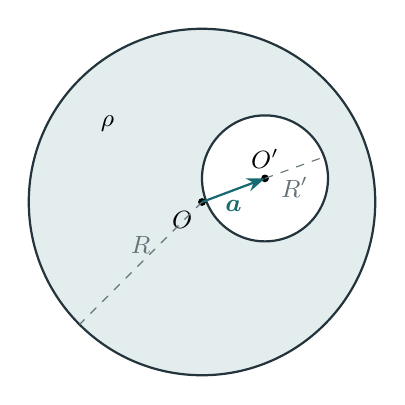
\begin{tikzpicture}[x=1cm,y=1cm]
\fill[accent!12] (0,0) circle (2.2);\fill[white] (.8,.3) circle (.8);\draw[object] (0,0) circle (2.2);\draw[object] (.8,.3) circle (.8);
\fill (0,0) circle (1.4pt) node[below left] {$O$};\fill (.8,.3) circle (1.4pt) node[above] {$O'$};
\draw[motion] (0,0)--(.8,.3) node[midway,below] {$\vect a$};\draw[guide] (0,0)--(225:2.2) node[midway,above] {$R$};
\draw[guide] (.8,.3)--({.8+.8*cos(20)},{.3+.8*sin(20)}) node[midway,below] {$R'$};\node at (-1.2,1) {$\rho$};
\end{tikzpicture}\figcaption{图 电1.9　空腔完全位于大球内部，剩余电荷固定不动。}\end{minipage}\end{center}

\Needspace{6\baselineskip}\subsection*{解答}

先求完整均匀带电球的内场。在球心为$O$、半径为$r$的高斯面上，球对称性保证场沿径向且处处等大，因而
\[E(r)\,4\pi r^2=\frac1{\varepsilon_0}\rho\frac{4\pi r^3}{3},\qquad
\vect E_{\rm full}(\vect r)=\frac\rho{3\varepsilon_0}\vect r\quad(r<R).\]
挖空操作可以等效为：保留体密度$+\rho$的完整大球，同时在球心$O'$处叠加半径$R'$、体密度$-\rho$的小球。空腔处的两种电荷相消，外面的电荷保持题设分布。
\begin{center}\begin{minipage}{0.97\linewidth}\centering
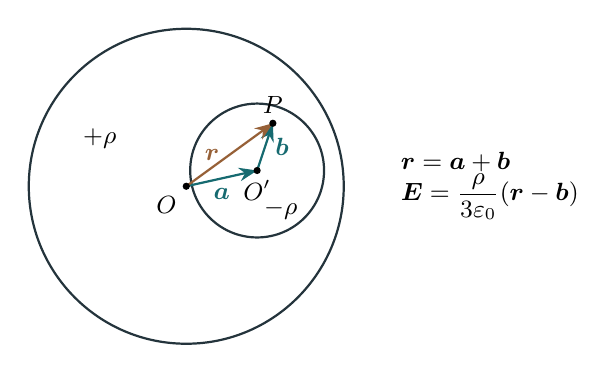
\begin{tikzpicture}[x=1cm,y=1cm]
\draw[object] (0,0) circle (2);\draw[object] (.9,.2) circle (.85);\coordinate (O) at (0,0);\coordinate (C) at (.9,.2);\coordinate (P) at (1.1,.8);
\draw[motion] (O)--(C) node[midway,below] {$\vect a$};\draw[motion] (C)--(P) node[midway,right] {$\vect b$};\draw[force] (O)--(P) node[midway,left] {$\vect r$};
\fill (O) circle (1.3pt) node[below left] {$O$};\fill (C) circle (1.3pt) node[below] {$O'$};\fill (P) circle (1.3pt) node[above] {$P$};
\node at (-1.1,.6) {$+\rho$};\node at (1.2,-.3) {$-\rho$};\node[right,align=left] at (2.6,0) {$\vect r=\vect a+\vect b$\\$\vect E=\dfrac{\rho}{3\varepsilon_0}(\vect r-\vect b)$};
\end{tikzpicture}\figcaption{解图 电1.9A　叠加完整的正电荷大球和负电荷小球，两项中随观察点变化的部分抵消。}\end{minipage}\end{center}
在空腔任取$P$，记$\vect r=\overrightarrow{OP}$、$\vect b=\overrightarrow{O'P}$。解图电1.9A中三个矢量满足
\[\vect r=\vect a+\vect b.\]
$P$同时位于两个完整球的内部，所以两项都可以使用内场公式：
\begin{align*}
\vect E(P)&=\frac\rho{3\varepsilon_0}\vect r-
\frac\rho{3\varepsilon_0}\vect b\\
&=\frac\rho{3\varepsilon_0}(\vect r-\vect b)
=\frac\rho{3\varepsilon_0}\vect a.
\end{align*}
特别地，在$P=O'$处，负电荷小球的场为零，也得到相同结果。故
\result{\vect E(O')=\vect E(P)=\frac\rho{3\varepsilon_0}\vect a.}
结果与$P$无关，证明空腔内场均匀。若$\rho>0$，方向为$O\to O'$；若$\rho<0$则相反。$a=0$时为同心空腔，内场退化为零；在空腔完全包含于大球的条件下，场与$R'$无关。

把两球的内部电势相加也可直接得到腔内的均匀场。忽略与位置无关的常数，两个球内部电势叠加为
\[\varphi(P)=C-\frac\rho{6\varepsilon_0}|\vect r|^2
+\frac\rho{6\varepsilon_0}|\vect r-\vect a|^2
=C'-\frac\rho{3\varepsilon_0}\vect a\cdot\vect r.\]
因此$-\nabla\varphi=\rho\vect a/(3\varepsilon_0)$，与上式相同。每个辅助球分别具有球对称性，因此各自使用球面高斯积分。合成后用位势的梯度得到真实空腔内的场。

还要说明“挖去电荷”与“挖去介质”的区别。本题把$\rho$规定为固定的给定电荷，采用真空中的叠加计算。若 $\rho$ 是可极化介质中的自由电荷，挖去介质还会改变介电常数和界面束缚电荷。若介电常数在全空间相同，仅去掉自由电荷而仍保留介质时，可按相同叠加得到$\rho\vect a/(3\varepsilon)$；再把小球区域的介质移走则需满足界面上切向$\vect E$连续、法向$\vect D$的跳变由自由面电荷决定。腔内的场由这些界面关系和外部条件共同确定。
\subsubsection*{以无穷远为零点的电势及其界面连续性}
前面的线性势还可保留全部常数，以无穷远为零势时，
均匀实心球的内部势为$\rho(3R^2-r^2)/(6\varepsilon_0)$。
与负小球势叠加，在腔内得到
\[
\begin{aligned}
\varphi(P)&=\frac\rho{6\varepsilon_0}
\left[3(R^2-R'^2)-|\vect r|^2+|\vect r-\vect a|^2\right]\\
&=\frac\rho{6\varepsilon_0}
\left[3(R^2-R'^2)+a^2-2\vect a\cdot\vect r\right].
\end{aligned}
\]
因此$\varphi(O')=\rho[3(R^2-R'^2)-a^2]/(6\varepsilon_0)$，
而$\varphi(P)-\varphi(O')=-\rho\vect a\cdot\vect b/(3\varepsilon_0)$。
腔内场由两球心的位移$\vect a$决定；腔半径$R'$则保留在电势的常数项以及剩余球体的总电量中。

在两个完整球的各自边界，内部势与外部点电荷势的值及法向导数均连续。
将它们相加所得全空间势，在剩余带电区满足$\nabla^2\varphi=-\rho/\varepsilon_0$，
在空腔及大球外满足$\nabla^2\varphi=0$，无穷远趋零。
空腔表面的面电荷密度为零，故表面两侧的电势及法向电场连续。体电荷密度则从带电区的$\rho$降到空腔内的零值。
若有另一套相同电荷和相同无穷远条件的解，差势全空间无源且边界项相消，
对差势用格林能量恒等式即得$\int|\nabla w|^2\dd V=0$。
故差场为零，叠加构造与对应边界条件一致且唯一。
这里各区域均为真空，电荷固定；因而全空间使用同一$\varepsilon_0$，上述连续关系与唯一性论证适用于这套电荷分布。

\subsubsection*{均匀介质中的真空球腔}
为看清极化的作用，单独考虑一个可精确求解的模型：
无限均匀线性介质的介电常数为$\varepsilon$，远处背景场为匀强场$\vect E_b$，
挖出半径b的球形真空腔，界面无自由面电荷。
解图电1.9B中，腔面同时分隔两种介电常数。沿背景场方向取极轴，分别写内外两区的势。

\begin{center}\begin{minipage}{.97\linewidth}\centering
\begin{tikzpicture}[x=1cm,y=1cm,font=\small]
\fill[accent!8] (-3,-1.7) rectangle(3,1.7);
\fill[white] (0,0) circle(1.2);\draw[object] (0,0) circle(1.2);
\draw[force] (-.65,0)--(.65,0) node[midway,above] {$\vect E_c$};
\draw[motion] (-2.8,.85)--(-1.5,.85) node[midway,above] {$\vect E_b$};
\draw[motion] (1.5,-.85)--(2.8,-.85) node[midway,above] {$\vect E_b$};
\node at (0,-.65) {$\varepsilon_0$};\node at (2,1.25) {$\varepsilon$};
\node at (0,2.15) {球形真空腔与均匀背景场};
\end{tikzpicture}
\figcaption{解图 电1.9B　无限线性介质中的球形腔；界面切向E连续，法向D连续。}
\end{minipage}\end{center}

以腔心为原点、背景场为极轴，用u记距腔心的距离，可设
\[
\varphi_{\rm in}=-A E_bu\cos\theta,\qquad
\varphi_{\rm out}=-E_bu\cos\theta+B E_b b^3\cos\theta/u^2.
\]
两式分别满足各自无电荷区的拉普拉斯方程；内势在中心有限，外势在远处恢复背景场。
在$u=b$处势连续给$A=1-B$，
法向D连续给$\varepsilon_0 A=\varepsilon(1+2B)$。
将腔面的两式联立，得到
\[
A=\frac{3\varepsilon}{2\varepsilon+\varepsilon_0},\qquad
B=\frac{\varepsilon_0-\varepsilon}{2\varepsilon+\varepsilon_0},\qquad
\vect E_c=\frac{3\varepsilon}{2\varepsilon+\varepsilon_0}\vect E_b.
\]
当$\varepsilon=\varepsilon_0$时因子为1；$\varepsilon>\varepsilon_0$时因子介于1与$3/2$之间，
因此场增强受有限上限约束。界面束缚电荷由求得的两侧场决定。如果介质在有限大球内并有自由体电荷，联立时还应同时用到外球面和内腔面的条件。


\Needspace{18\baselineskip}

\pdfbookmark[2]{第 10 题 八分之一带电球体的球心电场}{q10}

\section*{第 10 题\quad 八分之一带电球体的球心电场}\label{q:10}

用三个两两垂直且通过球心的平面，将半径为$R$的球体分成八等份。取第一卦限$x,y,z\ge0$的一份，使其均匀带电，体电荷密度为$\rho$。求球心$O$处电场的大小和方向。

\begin{center}\begin{minipage}{0.97\linewidth}\centering
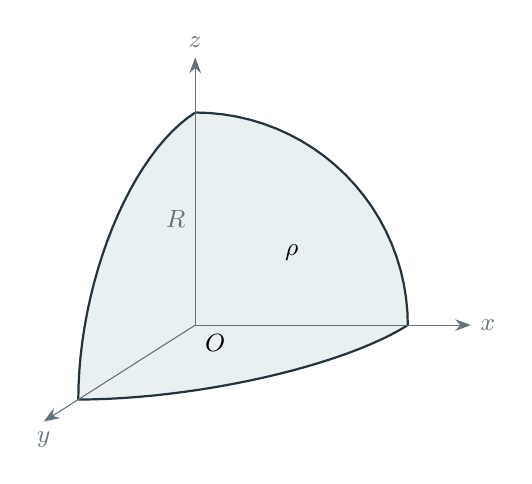
\begin{tikzpicture}[x={(1cm,0cm)},y={(-.55cm,-.35cm)},z={(0cm,1cm)},font=\small]
\fill[accent!10]
plot[domain=0:90,variable=\t] ({2.7*cos(\t)},0,{2.7*sin(\t)})
--plot[domain=90:0,variable=\t] (0,{2.7*cos(\t)},{2.7*sin(\t)})
--plot[domain=90:0,variable=\t] ({2.7*cos(\t)},{2.7*sin(\t)},0)--cycle;
\draw[object,domain=0:90,variable=\t] plot({2.7*cos(\t)},0,{2.7*sin(\t)});
\draw[object,domain=0:90,variable=\t] plot(0,{2.7*cos(\t)},{2.7*sin(\t)});
\draw[object,domain=0:90,variable=\t] plot({2.7*cos(\t)},{2.7*sin(\t)},0);
\draw[axis] (0,0,0)--(3.5,0,0) node[right] {$x$};
\draw[axis] (0,0,0)--(0,3.5,0) node[below] {$y$};
\draw[axis] (0,0,0)--(0,0,3.4) node[above] {$z$};
\draw[guide] (0,0,0)--(0,0,2.7) node[midway,left] {$R$};
\node[below right] at (0,0,0) {$O$};\node at (1.5,.5,1.1) {$\rho$};
\end{tikzpicture}\figcaption{图 电1.10　第一卦限的八分之一球体；三条直边互相垂直。}\end{minipage}\end{center}

\Needspace{6\baselineskip}\subsection*{解答}

记$k=1/(4\pi\varepsilon_0)$。解图电1.10B中的各薄壳沿同一空间对角线产生合场，因此可在求出一层的贡献后沿半径相加。先取$\rho>0$说明方向，最后对任意符号写出矢量结果。第一卦限的电荷元在球心产生的电场均有负的$x,y,z$分量；交换三个坐标不改变带电区域，所以三个合场分量相等。

先算均匀带电半球面在球心的场。设其半径为$r$、面电荷密度为$\sigma$，半球面位于$x\le0$侧。对面元$\dd S$，其场在$x$方向的分量为
\[\dd E_x=\frac{k\sigma}{r^2}\cos\theta\,\dd S
=\frac{k\sigma}{r^2}\dd S_\perp.\]
\begin{center}\begin{minipage}{0.97\linewidth}\centering
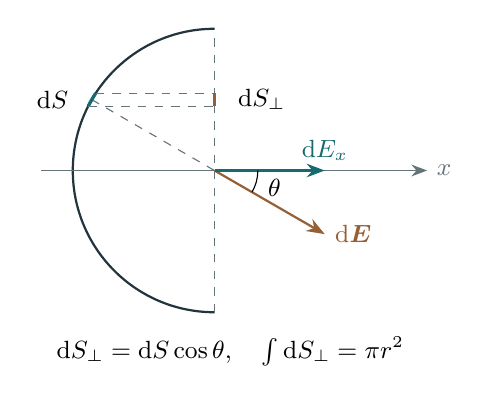
\begin{tikzpicture}[x=1cm,y=1cm,font=\small]
\draw[object] (0,1.8) arc(90:270:1.8);\draw[guide] (0,-1.8)--(0,1.8);
\draw[axis] (-2.2,0)--(2.7,0) node[right] {$x$};
\coordinate (D) at (150:1.8);\draw[guide] (D)--(0,0);
\draw[force] (0,0)--(1.4,{-1.4/sqrt(3)}) node[right] {$\dd\vect E$};
\draw[motion] (0,0)--(1.4,0) node[above] {$\dd E_x$};
\coordinate (D1) at (153:1.8);\coordinate (D2) at (147:1.8);
\draw[very thick,accent] (D1) arc(153:147:1.8);
\draw[very thick,warm] (0,{1.8*sin(153)})--(0,{1.8*sin(147)});
\draw[guide] (D1)--(0,{1.8*sin(153)});\draw[guide] (D2)--(0,{1.8*sin(147)});
\node[left=5pt] at (D) {$\dd S$};\node[right=5pt] at (0,.9) {$\dd S_\perp$};
\draw (.55,0) arc(0:-30:.55);\node at (.76,-.22) {$\theta$};
\node at (.2,-2.3) {$\dd S_\perp=\dd S\cos\theta,\quad \int\dd S_\perp=\pi r^2$};
\end{tikzpicture}\figcaption{解图 电1.10A　半球面的轴向场可用底圆投影面积计算；图中只画过轴截面。}\end{minipage}\end{center}
解图电1.10A中$\dd S_\perp$是面元在垂直于$x$轴的底圆上的投影。整个半球面恰好投影覆盖一个圆盘，故
\[E_{\rm hemi}=\frac{k\sigma}{r^2}\pi r^2=k\pi\sigma=\frac\sigma{4\varepsilon_0}.\]
把一个半球面分成四个八分之一球面，四份对$x$分量的贡献相等，其他分量成对抵消。因此单份八分之一球面的一个分量大小为
\[|E_x^{\rm oct}|=\frac14E_{\rm hemi}=\frac\sigma{16\varepsilon_0}.\]
再由三个坐标的置换对称性，$|E_x^{\rm oct}|=|E_y^{\rm oct}|=|E_z^{\rm oct}|$，于是
\[|\vect E^{\rm oct}|=\frac{\sqrt3\,\sigma}{16\varepsilon_0}.\]
这里四份八分之一球面组成半球，四份只留下同轴分量，总场为单份轴向分量的四倍。
\begin{center}\begin{minipage}{0.97\linewidth}\centering
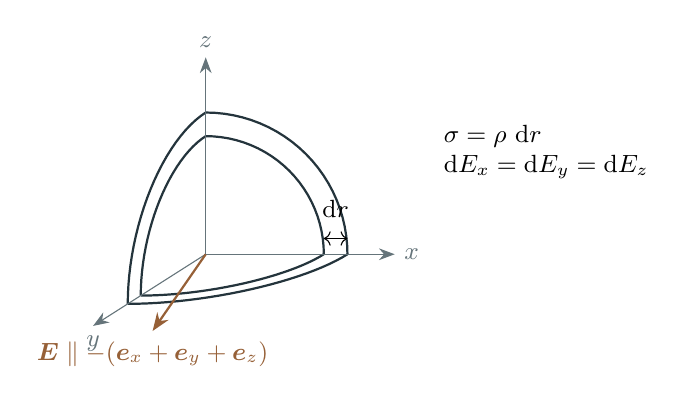
\begin{tikzpicture}[x={(1cm,0cm)},y={(-.55cm,-.35cm)},z={(0cm,1cm)},font=\small]
\foreach \r in {1.5,1.8}{
\draw[object,domain=0:90,variable=\t] plot({\r*cos(\t)},0,{\r*sin(\t)});
\draw[object,domain=0:90,variable=\t] plot(0,{\r*cos(\t)},{\r*sin(\t)});
\draw[object,domain=0:90,variable=\t] plot({\r*cos(\t)},{\r*sin(\t)},0);}
\draw[axis] (0,0,0)--(2.4,0,0) node[right] {$x$};
\draw[axis] (0,0,0)--(0,2.6,0) node[below] {$y$};
\draw[axis] (0,0,0)--(0,0,2.5) node[above] {$z$};
\draw[<->] (1.5,0,.2)--(1.8,0,.2) node[midway,above=4pt] {$\dd r$};
\draw[force] (0,0,0)--(-1.5,-1.5,-1.5) node[below] {$\vect E\parallel-(\vect e_x+\vect e_y+\vect e_z)$};
\node[right,align=left] at (2.9,0,1.3) {$\sigma=\rho\,\dd r$\\$\dd E_x=\dd E_y=\dd E_z$};
\end{tikzpicture}\figcaption{解图 电1.10B　各薄壳的合场沿同一空间对角线，分量可逐层相加。}\end{minipage}\end{center}
将八分之一球体分为半径$r$、厚度$\dd r$的薄壳。设该层球面面积为$S(r)$，则
\[\dd Q=\rho S(r)\dd r,\qquad \sigma(r)=\frac{\dd Q}{S(r)}=\rho\dd r.\]
每层电场方向相同，均沿第一卦限空间对角线的反方向，可以直接积分分量：
\[\dd\vect E=-\frac{\rho\dd r}{16\varepsilon_0}
(\vect e_x+\vect e_y+\vect e_z).\]
从$r=0$积到$R$，得到
\result{\vect E(O)=-\frac{\rho R}{16\varepsilon_0}(\vect e_x+\vect e_y+\vect e_z),
\qquad E_0=\frac{\sqrt3\,|\rho|R}{16\varepsilon_0}.}
$\rho>0$时电场背离带电卦限，$\rho<0$时反向。半径小于$\epsilon$的核心给出的场为$-\rho\epsilon(\vect e_x+\vect e_y+\vect e_z)/(16\varepsilon_0)$，随$\epsilon\to0$线性减小。这里的$r^{-2}$与薄层面积中的$r^2$相消。

球坐标积分可直接显示分量相同的几何因子。取$\theta$为相对$+z$轴的极角、$\phi$为从$+x$轴起算的方位角，
第一卦限对应$0\le\theta,\phi\le\pi/2$。
体积元$\dd V=r^2\sin\theta\dd r\dd\theta\dd\phi$，从电荷元指向球心的单位矢量之$x$分量为$-\sin\theta\cos\phi$，故
\[
\dd E_x=-\frac{k\rho\dd V}{r^2}\sin\theta\cos\phi
=-k\rho\sin^2\theta\cos\phi\dd r\dd\theta\dd\phi.
\]
其中一个$\sin\theta$来自体积元，另一个来自方向投影。分离三个积分便有
\[E_x=-k\rho\int_0^R\dd r\int_0^{\pi/2}\sin^2\theta\,\dd\theta
\int_0^{\pi/2}\cos\phi\,\dd\phi
=-k\rho R\frac\pi4=-\frac{\rho R}{16\varepsilon_0}.\]
另外两个分量由坐标对称性相同。两个方法都把径向部分化为厚度积分，差别在角向分量的计算。
\subsubsection*{面积投影与四份分量关系的完整几何说明}
解图电1.10A只画半球的过轴截面，图中的短弧代表一个微小面元所在的局部位置，
将截面绕 $x$ 轴转到任一方位角，可以找到对应的面元；
这样的旋转不改变面元面积、到O的距离和电场的x分量。
与该面元绕轴对称的其他面元，其横向分量在整圈求和中抵消，轴向分量相加。
因此只计算每元的x投影，已经包含整个半球的方位对称性。

面元可视为微小平面，法线沿球半径。
其法线与投影方向的夹角恰与场元和x轴的夹角对应，
正投影面积才是$\dd S_\perp=\dd S\cos\theta$。
半球在底圆上恰好投影一次：底圆内每一点沿投影线只对应这一半球上的一个点。
赤道处投影退化为零面积的边界，不会额外贡献一层面积，
所有面元投影相加，得底圆盘面积 $\pi r^2$。
面电荷的反平方因子与底圆面积中的$r^2$抵消，
这才说明同密度半球面在球心的场与r无关。

再把半球分成四份，须比较同一个坐标分量。
四份在对称轴上的分量相等且同向，另外两方向则成对相消，
因此半球合场是单份轴向分量的4倍。
单份合场沿空间对角线，其大小是任一分量的$\sqrt3$倍，
因子4用于同轴分量，因子 $\sqrt3$ 用于把等大的三个正交分量合成。
第一卦限的正电荷在O产生三个负分量，解图电1.10B的箭头应背离带电卦限。
若体密度变负，三个分量一起反向，大小公式使用$|\rho|$。

\subsubsection*{分层求和与最内层的收敛}
不求角积分也能完成主解：把半径区间划成许多小层，层厚为$\Delta r_i$。
在远离零半径的薄层上，体电量为$\rho S(r_i)\Delta r_i$，
等效面密度为$\rho\Delta r_i$，故该层某个分量的主阶贡献为
$-\rho\Delta r_i/(16\varepsilon_0)$。
这些层在空间对角线方向的贡献同向，可以直接作矢量求和：
\[
\vect E_N\longrightarrow-\frac{\rho}{16\varepsilon_0}
(\vect e_x+\vect e_y+\vect e_z)\lim_{N\to\infty}\sum_i\Delta r_i
=-\frac{\rho R}{16\varepsilon_0}(\vect e_x+\vect e_y+\vect e_z).
\]
每层贡献正比于径向厚度，各层厚度相加为 $R$。
这条几何与薄层路线不需要求任何三角函数的原函数；
采用球坐标时，面元投影所用的角向因子由三重积分给出。

对半径趋零处单独估计，将 $0\le r<\epsilon$ 取为一个小核心。
其场大小不超过所有场元大小之和，后者为
\[
\int_{r<\epsilon,\,\rm oct}\frac{k|\rho|}{r^2}\dd V
=k|\rho|\frac\pi2\,\epsilon\longrightarrow0.
\]
故先使其余层足够薄、再令$\epsilon\to0$，可恢复从球心开始的整个球体。
该上界与核心半径成正比，所以令 $\epsilon\to0$ 恢复完整的积分。

\subsubsection*{内层球体的累计电量和球心场}
解图电1.10C比较同卦限内半径uR核心的两种累计比例。
均匀密度下电量比例为$u^3$，球心场贡献比例却为u，
因为各薄层的面积增长已与距离平方衰减抵消。
例如内半径$R/2$包含总电量的$1/8$，却贡献总球心场的一半。

\begin{center}\begin{minipage}{.97\linewidth}\centering
\begin{tikzpicture}[x=4.6cm,y=2.6cm,font=\small]
\draw[axis] (0,0)--(1.25,0) node[right] {$u=r/R$};
\draw[axis] (0,-.08)--(0,1.35) node[above] {累计比例};
\draw[traj] (0,0)--(1,1);
\draw[brown,thick,dashed,domain=0:1,samples=80] plot(\x,{pow(\x,3)});
\node at (.37,.85) {场：$u$};\node at (.83,.32) {电量：$u^3$};
\draw[guide] (.5,0)--(.5,.5)--(0,.5) node[left] {$1/2$};
\node[below] at (.5,0) {$1/2$};\node[below] at (1,0) {$1$};\node[left] at (0,1) {$1$};
\end{tikzpicture}
\figcaption{解图 电1.10C　均匀八分之一球体的核心累计场与累计电量；归一化要求$\rho\ne0$。}
\end{minipage}\end{center}

固定总电量$Q=\pi\rho R^3/6$时，可改写
$E_0=3\sqrt3|Q|/(8\pi\varepsilon_0R^2)$；
固定体密度时才有$E_0\propto R$，两条尺度关系分别取固定总量和固定密度。
完整球的八个卦限各自产生非零场。关于球心中心对称的两个卦限产生等大反向的场，各对相消后完整球在球心的总场为零。


\Needspace{18\baselineskip}

\pdfbookmark[2]{第 11 题 匀强电场中的连续弹性碰撞}{q11}

\section*{第 11 题\quad 匀强电场中的连续弹性碰撞}\label{q:11}

质量均为$m$的两个小球$A,B$静止在同一直线上，初始间距为$l$。$A$带正电$Q$，$B$不带电；沿$A$指向$B$的方向存在匀强电场$E$。两球发生完全弹性正碰，碰撞时不交换电荷，忽略重力及其他相互作用。证明相邻两次碰撞的时间间隔相同，并求此间隔。

\begin{center}\begin{minipage}{0.97\linewidth}\centering
\begin{tikzpicture}[x=1cm,y=1cm]
\draw[guide] (-.5,0)--(6,0);\fill[accent] (0,0) circle (3pt) node[above] {$A:m,Q$};\fill (4.5,0) circle (3pt) node[above] {$B:m,0$};
\draw[<->] (0,-.7)--(4.5,-.7) node[midway,below] {$l$};\draw[force] (1.2,1)--(3.5,1) node[midway,above] {$\vect E$};
\end{tikzpicture}\figcaption{图 电1.11　两球初始静止；只有A持续受到向右的电力。}\end{minipage}\end{center}

\Needspace{6\baselineskip}\subsection*{解答}

电场只使$A$加速，记$a=QE/m$。首次相碰前，$B$不动，因此
\[l=\frac12at_0^2,\qquad t_0=\sqrt{\frac{2l}{a}},\qquad v_0=at_0=\sqrt{2al}.\]
对于质量相同的一维完全弹性碰撞，动量、动能守恒给出碰后速度互换。因此第一次碰撞后$A$静止、$B$以$v_0$向右运动。
\begin{center}\begin{minipage}{0.97\linewidth}\centering
\begin{tikzpicture}[x=5cm,y=2cm,font=\small]
\draw[axis] (-.06,0)--(1.25,0) node[right] {$u=\tau/T$};
\draw[axis] (0,-1.2)--(0,.35) node[above] {$s/l$};
\draw[traj,domain=0:1,samples=100] plot(\x,{4*\x*(\x-1)});
\draw[guide] (.5,0)--(.5,-1)--(0,-1) node[left] {$-1$};
\node[above] at (.5,0) {$1/2$};\node[above] at (1,0) {$1$};
\node at (.7,-1.5) {$\dot s(0)=-v_0,\quad\dot s(T)=v_0$};
\end{tikzpicture}\figcaption{解图 电1.11A　碰后相对位置是一条抛物线，下一次相碰是第二个零点。}\end{minipage}\end{center}
在随$B$匀速运动的参考系中，以一次碰撞为计时零点，令$s=x_A-x_B$。第一次碰撞刚结束时$s=0,\dot s=-v_0$，而相对加速度仍为$a$，所以
\[s(\tau)=-v_0\tau+\frac12a\tau^2.\]
解图电1.11A中曲线先降后升；除$\tau=0$外，另一零点为$T=2v_0/a$。在$\tau=T/2$，两球间距最大，为$v_0^2/(2a)=l$；下一次碰前的相对速度为$-v_0+aT=v_0$。

碰撞使两球速度互换，因而相对速度再次由$+v_0$变成$-v_0$。每一轮都具有相同的相对初态和相对加速度，以上过程可逐次重复。相邻碰撞的恒定间隔因而为
\result{T=2\sqrt{\frac{2ml}{QE}}.}
也可直接归纳实验室系速度：第$n$次碰撞前，$v_A=nv_0,v_B=(n-1)v_0$；碰后变成$v_A=(n-1)v_0,v_B=nv_0$。两球的共同平移越来越快，但它们的相对运动不变。第$n$次碰撞时刻为$t_n=t_0+(n-1)T=(2n-1)t_0$；从静止释放到第一次碰撞用 $t_0$，此后每个完整的分离、追及过程用 $2t_0$。
\subsubsection*{弹性正碰为什么交换速度}
先把碰撞本身与两次碰撞之间的运动分开。
记碰前速度为$u_A,u_B$，碰后为$w_A,w_B$。
在理想瞬时碰撞中，外电场力的冲量随碰撞时间趋零，可对两球碰撞过程列
\[
u_A+u_B=w_A+w_B,\qquad
u_A^2+u_B^2=w_A^2+w_B^2.
\]
由两式得$(w_A-w_B)^2=(u_A-u_B)^2$。
接触前两球相互靠近，反弹后二者分开，故相对速度取反号的分支，
$w_A-w_B=-(u_A-u_B)$，与动量式联立便是$w_A=u_B,w_B=u_A$。
同号的另一代数支给速度保持，反号支对应接触后分开。
碰撞瞬时的外冲量及功可略；自由飞行的总动量由外冲量改变、总动能由外力功改变。

\subsubsection*{逐次选择惯性系的完整对应}
第一次碰后，实验室系中A暂时静止，B以$v_0$匀速向右。
选择以恒速$v_0$向右平移的$S_1$系，B在本轮自由飞行中静止，
A初速为$-v_0$、加速度仍为$+a$。
在此系中A先向左减速，经过$v_0/a=t_0$停下，退后距离为
\[
v_0t_0-\frac12at_0^2=\frac{v_0^2}{2a}=l.
\]
随后A从相距l的位置由静止向右加速，再经过$t_0$、以$+v_0$回到B。
去程和回程时间相同，给相邻碰撞间隔$2t_0$；
这与解图电1.11A抛物线在最低点两侧的时间对称完全对应。

第二次碰撞在$S_1$中仍交换速度，因此碰后A静止、B以$+v_0$离开。
此时另选相对于$S_1$以$v_0$平移的惯性系$S_2$，
又得到B静止、A以$-v_0$出发及加速度$+a$的同一初值问题。
以后每次碰撞后都可这样重新选择恒速系，从每次碰后开始，局部参考系中的运动方程、初态与终止条件都重现。

$S_1,S_2,\ldots$ 分别是以该段 B 速度匀速平移的惯性系。
B在碰撞时速度突变，只在每段自由飞行中匀速；
重新选系正是为避开这个速度突变，同时保留伽利略变换下不变的时间间隔和相对加速度。
直接用 $s=x_A-x_B$ 时，两个位置中的共同平移自动相消，得到同一相对初值问题。

\subsubsection*{每次碰撞前后的实验室系速度}
解图电1.11B画实验室系中的两球速度，时间按$t_0$归一。
折线A在自由飞行段斜率相同，B呈阶梯状；每次碰撞两者交换高度，
但后续碰撞的时距始终为$2t_0$。

\begin{center}\begin{minipage}{.97\linewidth}\centering
\begin{tikzpicture}[x=1.05cm,y=.85cm,font=\small]
\draw[axis] (0,0)--(7.6,0) node[right] {$t/t_0$};
\draw[axis] (0,-.15)--(0,4.8) node[above] {$v/v_0$};
\draw[traj] (0,0)--(1,1)--(1,0)--(3,2)--(3,1)--(5,3)--(5,2)--(7,4);
\draw[brown,thick,dashed] (0,0)--(1,0)--(1,1)--(3,1)--(3,2)--(5,2)--(5,3)--(7,3);
\foreach \x in {1,3,5}{\draw[guide] (\x,0) node[below] {$\x$}--(\x,4.2);}
\node at (5.8,4.5) {实线A，虚线B};\node[left] at (0,1) {$1$};
\end{tikzpicture}
\figcaption{解图 电1.11B　实验室系两速度线的高度逐次上升，各轮相对速度曲线等形。}
\end{minipage}\end{center}

具体地，假设第n次碰后$w_A=(n-1)v_0,w_B=nv_0$，
则下一段相对初速仍为$-v_0$、相对加速度仍为a。
经过$T=2v_0/a$，A的速度成为$(n+1)v_0$，B仍为$nv_0$，
相对速度为$+v_0$且两者位置再相同。
交换速度后就是第$n+1$轮的初态，归纳闭合。
解图B 的每段中点，两球在实验室系中同速，速度为 $nv_0$，相对速度为零。在这一时刻，两球刚从分离转为追赶，间距达到 $l$。若从第 $n$ 次相碰的共同位置 $x_n$ 计位移，这一段的两个实验室系位置就是
\[
x_A=x_n+(n-1)v_0\tau+\tfrac12a\tau^2,\qquad
x_B=x_n+nv_0\tau .
\]
在 $\tau=t_0$ 时，B已前进 $2nl$，A前进 $(2n-1)l$，两者相差 $l$。共同前进的距离随轮次增大，但这两个位置相减后，保留的是解图电1.11A所画的同一条相对位置曲线。

以 $A$ 起点为坐标零点、$B$ 初始位置为 $l$，由质心运动求各次碰撞的位置。
质心$X=(x_A+x_B)/2$满足$2m\ddot X=QE$，
碰撞不改变系统总动量，所以质心速度在碰撞时连续，
从释放起一直有
\[
X(t)=\frac l2+\frac a4t^2.
\]
碰撞时$s=0$，两球共同位置就是质心位置。
代入$t_n=(2n-1)t_0$得
\[
x_n=\frac l2+\frac a4(2n-1)^2t_0^2
=[1+2n(n-1)]l,
\quad x_{n+1}-x_n=4nl.
\]
这与第n次碰后B以$nv_0$飞行$2t_0$的位移相同。
每轮总动量增加$QE\,T=2mv_0$，
总动能增加$QE(x_{n+1}-x_n)=4nQEl$，均由持续外电力提供。
相对速度在碰撞时反号，使相对运动每隔 $T$ 复现。共同速度则随外力冲量增长。


\Needspace{18\baselineskip}

\pdfbookmark[2]{第 12 题 带电厚板两侧的分段运动}{q12}

\section*{第 12 题\quad 带电厚板两侧的分段运动}\label{q:12}

无限大均匀带电厚板占据$-d\le x\le d$，体电荷密度为$\rho>0$。质量$m$、电荷$q<0$的质点从$x=2d$处静止释放，仅受厚板的电场力。求它第一次到达厚板中面$x=0$的时间。电荷分布固定，按真空静电定律计算。

\begin{center}\begin{minipage}{0.97\linewidth}\centering
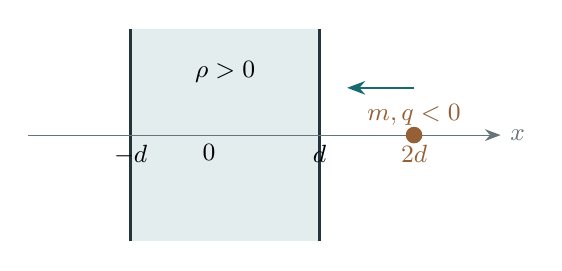
\begin{tikzpicture}[x=1cm,y=1cm]
\fill[accent!12] (-1.2,-1.35) rectangle (1.2,1.35);\draw[object] (-1.2,-1.35)--(-1.2,1.35) (1.2,-1.35)--(1.2,1.35);
\draw[axis] (-2.5,0)--(3.5,0) node[right] {$x$};\node[below] at (-1.2,0) {$-d$};\node[below] at (1.2,0) {$d$};\node[below left] at (0,0) {$0$};\node at (0,.8) {$\rho>0$};
\fill[warm] (2.4,0) circle (3pt) node[above] {$m,q<0$} node[below] {$2d$};\draw[motion] (2.4,.6)--(1.55,.6);
\end{tikzpicture}\figcaption{图 电1.12　粒子先经过板外匀强场，再进入板内线性场。}\end{minipage}\end{center}

\Needspace{6\baselineskip}\subsection*{解答}

厚板关于中面对称，电场垂直板面。取两底面在$\pm x$、面积为$S$的高斯柱，$0\le x\le d$时
\[2E(x)S=\frac{2xS\rho}{\varepsilon_0},\]
故$E_x=\rho x/\varepsilon_0$。板外高斯柱包围的电荷不再随$x$增加，得到
\[E_x(x)=\begin{cases}\rho d/\varepsilon_0,&x>d,\\\rho x/\varepsilon_0,&|x|\le d,\\-\rho d/\varepsilon_0,&x<-d.\end{cases}\]
记$\omega^2=|q|\rho/(m\varepsilon_0)$。负电荷受力指向中面，但板外为恒力、板内才是线性回复力。
\begin{center}\begin{minipage}{0.97\linewidth}\centering
\begin{tikzpicture}[x=1cm,y=1cm]
\draw[axis] (-3,0)--(3.2,0) node[right] {$x$};\draw[axis] (0,-1.6)--(0,1.8) node[above] {$E_x$};
\draw[traj] (-2.8,-1.1)--(-1.2,-1.1)--(1.2,1.1)--(2.8,1.1);\draw[guide] (-1.2,0)--(-1.2,-1.1) (1.2,0)--(1.2,1.1)--(0,1.1);
\node[below right] at (1.2,0) {$d$};\node[above left] at (-1.2,0) {$-d$};\node[left] at (0,1.1) {$\rho d/\varepsilon_0$};\node at (0,-2) {$a_x=qE_x/m$};
\end{tikzpicture}\figcaption{解图 电1.12A　场在板面连续，板外恒定、板内与位置成正比。}\end{minipage}\end{center}
解图电1.12A中，$x=\pm d$连接水平支与斜直线支，场强在板面连续，斜率却改变。粒子越过板面时速度也连续，用同一个入板速度把板外匀加速与板内简谐两段连接起来。

从$2d$到$d$，位移为$-d$、加速度为$-\omega^2d$，因此
\[t_1=\frac{\sqrt2}{\omega},\qquad v_d=-\omega^2dt_1=-\sqrt2\omega d.\]
进入板内后重新计时为$\tau$，满足$\ddot x+\omega^2x=0$，但初速度不为零。由$x(0)=d,\dot x(0)=v_d$，
\[x=d\cos\omega\tau-\sqrt2d\sin\omega\tau.\]
第一次到达$x=0$时$0<\omega t_2<\pi/2$，故
\[\tan\omega t_2=\frac1{\sqrt2},\qquad
t_2=\frac1\omega\arctan\frac1{\sqrt2}=\frac1\omega\arcsin\frac1{\sqrt3}.\]
\Needspace{10\baselineskip}
总时间为
\result{t=\sqrt{\frac{m\varepsilon_0}{|q|\rho}}\left(\sqrt2+\arcsin\frac1{\sqrt3}\right).}
由板内能量积分$v^2+\omega^2x^2=v_d^2+\omega^2d^2$，中心速率为$\sqrt3\omega d$。入板时已有速率 $\sqrt2\omega d$，因此从板面到中面经过的相位小于 $\pi/2$。结果与$d$无关，是因为起点到板面的距离和板外加速度都正比于$d$，而板内的初始相位也不随$d$变化。
\subsubsection*{两侧电荷层给出的板内场}
除高斯柱外，还可按解图电1.12A所示的观察坐标x，将厚板分为$[-d,x]$与$[x,d]$两部分。
在$0<x<d$时，左侧部分的等效面电荷密度为$\sigma_{\rm I}=\rho(d+x)$，
右侧为$\sigma_{\rm II}=\rho(d-x)$。
它们的场分别向右、向左，两个大小为
\[
E_{\rm I}=\frac{\rho(d+x)}{2\varepsilon_0},\qquad
E_{\rm II}=\frac{\rho(d-x)}{2\varepsilon_0}.
\]
按同一$+x$方向相减得到$E_x=E_{\rm I}-E_{\rm II}=\rho x/\varepsilon_0>0$。
负粒子受力的轴向分量则是$qE_x=-m\omega^2x<0$。
所以右半板内的电场向右，负电荷所受的力向左。上式的负号表示沿 $x$ 负向，力的大小取分量的绝对值。
粒子逐渐接近中面时，加速度仍向左，但其大小从$\omega^2d$减为零，
速度的大小却继续增加，到中面达到最大值。

\subsubsection*{初始相位与两个计时零点}
把板内解改写成$x=A\cos(\omega\tau+\varphi)$，
由入板的两个初值逐式得到
\[
A\cos\varphi=d,\qquad
-A\omega\sin\varphi=-\sqrt2\omega d.
\]
第二式由余弦位移求导，负号来自余弦的导数。
平方相加给$A=\sqrt3d$，同时$\cos\varphi>0,\sin\varphi>0$，
所以首次进入板内时的相位在第一象限，$\varphi=\arctan\sqrt2$。
随后相位增加，到第一次过中面为$\pi/2$，故
\[
\omega t_2=\frac\pi2-\arctan\sqrt2
=\arctan\frac1{\sqrt2}=\arcsin\frac1{\sqrt3}.
\]
释放时实验室时间为$t=0$，入板时为$t=t_1$而$\tau=0$，
两者的关系是$\tau=t-t_1$。
在$t_1$两侧，位置都为d、速度都为$-\sqrt2\omega d$，
加速度也都为$-\omega^2d$；力连续而力对位置的导数改变。
板内的局部时钟从入板起计，入板速度延续了板外运动的末态。

\begin{center}\begin{minipage}{.97\linewidth}\centering
\begin{tikzpicture}[x=3cm,y=1.25cm,font=\small]
\draw[axis] (0,0)--(2.5,0) node[right] {$u=\omega t$};
\draw[axis] (0,-.1)--(0,2.55) node[above] {$x/d$};
\draw[traj,domain=0:1.414213562,samples=80] plot(\x,{2-\x*\x/2});
\draw[brown,thick,domain=1.414213562:2.029693271,samples=80]
plot(\x,{cos((\x-sqrt(2))*180/pi)-sqrt(2)*sin((\x-sqrt(2))*180/pi)});
\draw[guide] (1.414213562,0) node[below] {$\sqrt2$}--(1.414213562,1)--(0,1) node[left] {$1$};
\node[left] at (0,2) {$2$};\node at (.65,2.25) {板外匀加速};\node at (1.95,1.85) {板内线性力};
\end{tikzpicture}
\figcaption{解图 电1.12B　从释放到中面的实际位置曲线；在$x=d$处接续位置、速度和加速度。}
\end{minipage}\end{center}
解图电1.12B两段位置曲线在板面处以同一非零斜率接续。
末端斜率对应中心速度$-\sqrt3\omega d$；
过中面时加速度为零，速率达到最大。

\subsubsection*{分段势能与从释放点到中面的时间积分}
以中面处粒子势能为零，完整的连续势能为
\[
U(x)=m\omega^2\begin{cases}x^2/2,&|x|\le d,\\d|x|-d^2/2,&|x|\ge d.\end{cases}
\]
释放处$x=2d$给总能量$E=3m\omega^2d^2/2$。
板外的速率由能量式给$|\dot x|=\omega\sqrt{2d(2d-x)}$，
所以$t_1=\int_d^{2d}\dd x/[\omega\sqrt{2d(2d-x)}]=\sqrt2/\omega$。
板内则有$|\dot x|=\omega\sqrt{3d^2-x^2}$，
\[
t_2=\frac1\omega\int_0^d\frac{\dd x}{\sqrt{3d^2-x^2}}
=\frac1\omega\left[\arcsin\frac{x}{\sqrt3d}\right]_0^d
=\frac1\omega\arcsin\frac1{\sqrt3}.
\]
板外与板内的能量积分分别复得$t_1,t_2$，并给出中心速率$\sqrt3\omega d$。

\begin{center}\begin{minipage}{.97\linewidth}\centering
\begin{tikzpicture}[x=1.7cm,y=1.4cm,font=\small]
\draw[axis] (-2.3,0)--(2.55,0) node[right] {$\xi=x/d$};
\draw[axis] (0,-.12)--(0,2.65) node[above] {$U/(m\omega^2d^2)$};
\draw[traj] (-2.1,1.6)--(-1,.5);
\draw[traj,domain=-1:1,samples=80] plot(\x,{\x*\x/2});
\draw[traj] (1,.5)--(2.1,1.6);
\draw[brown,dashed,domain=1:2.1,samples=60] plot(\x,{\x*\x/2});
\draw[guide] (-2,1.5)--(2,1.5);\node[left] at (0,1.5) {$3/2$};
\draw[guide] (2,0) node[below right] {$2$}--(2,1.5);
\draw[guide] (1.732050808,0) node[below left] {$\sqrt3$}--(1.732050808,1.5);
\node at (-1.1,2.25) {实线：实际势能};\node at (1.4,2.45) {虚线：抛物线延长};
\end{tikzpicture}
\figcaption{解图 电1.12C　实际转折点在$2d$；形式振幅$\sqrt3d$属于延长的抛物线势，超出板内力律范围。}
\end{minipage}\end{center}
在解图电1.12C中，延长的板内抛物线在 $\sqrt3d$ 与能量线相交，用于确定板内相位。实际板外势的交点给真正转折位置；
真实往复仍回到$\pm2d$，由中面对称与时间反演，其周期为首次到中面时间的4倍。
最后令$\xi=x/d,u=\omega t$，两段方程分别化为$\xi''=-1$和$\xi''=-\xi$，
初态为$\xi(0)=2,\xi'(0)=0$，其中不再含d。
这说明固定$\rho,q,m$且保持起点为$2d$时，厚度改变虽使路程和速度都按d缩放，
到中面的时间却不变；若只保持绝对起点不变，则没有同样的缩放条件。


\Needspace{18\baselineskip}

\pdfbookmark[2]{第 13 题 非均匀带电圆环的平衡与振动}{q13}

\section*{第 13 题\quad 非均匀带电圆环的平衡与振动}\label{q:13}

半径$R$的刚性绝缘细圆环带正电$Q$，电荷可非均匀地固定分布。圆环在$xy$平面内，圆心为$O$。
\begin{enumerate}\item 怎样选择沿圆周的线电荷密度，使一个非零点电荷能沿直径$AOB$的内部作匀速直线运动？以从$+x$轴量起的极角$\phi$表示结果。
\item 将点电荷$Q_1$放在$x=-r_1$，$r_1>R$，已知$|Q_1|=\nu Q$。能否在$x=r_2>R$再放一个点电荷$Q_2$，使两个点电荷与圆环在均无支撑力的情况下同时平衡？求电荷符号、$Q_2,r_2$及参数条件。
\item 固定上述两个点电荷的位置，再把它们同时变号，圆环的电荷不变。圆环质量为$m$，质量分布均匀。将圆环沿$x$轴移动很小的距离$\delta$后静止释放，求其轴向小振动。\end{enumerate}

\begin{center}\begin{minipage}{0.97\linewidth}\centering
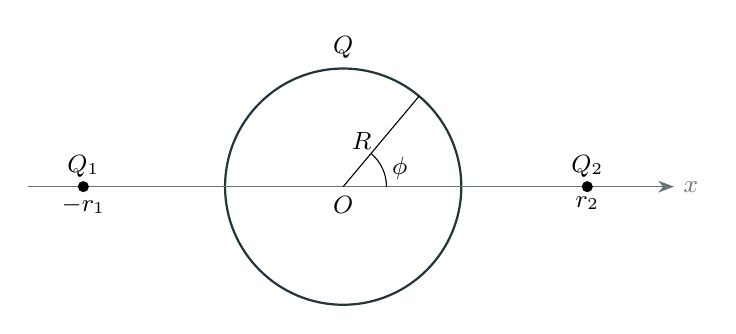
\begin{tikzpicture}[x=1cm,y=1cm]
\draw[object] (0,0) circle (1.5);\draw[axis] (-4,0)--(4.2,0) node[right] {$x$};\node[below] at (0,0) {$O$};
\fill (-3.3,0) circle (2pt) node[above] {$Q_1$} node[below] {$-r_1$};\fill (3.1,0) circle (2pt) node[above] {$Q_2$} node[below] {$r_2$};
\draw (0,0)--(50:1.5) node[midway,left] {$R$};\draw (.55,0) arc (0:50:.55) node[midway,right] {$\phi$};\node[above] at (0,1.5) {$Q$};
\end{tikzpicture}\figcaption{图 电1.13　点电荷位于环面内的一条直径延长线上。}\end{minipage}\end{center}

\Needspace{6\baselineskip}\subsection*{解答}

\textbf{（1）构造直径上的零场。} 先考虑半径$R$、总电荷$Q$的均匀球面。按与$x$轴夹角$\phi$分成细纬圈；其电荷为
\[\dd Q_{\rm band}=\frac{Q}{4\pi R^2}\,2\pi R^2\sin\phi\dd\phi
=\frac Q2\sin\phi\dd\phi,\qquad0\le\phi\le\pi.\]
按解图电1.13A，把每个纬圈的电荷等分到圆环上、下两个同$x$坐标的弧元。对$x$轴上的观察点，纬圈各点的距离和库仑场的$x$投影因子相同；上、下弧元又消去横向场，因此这一转移保持$x$轴上的电场和电势。
\begin{center}\begin{minipage}{0.97\linewidth}\centering
\begin{tikzpicture}[x=1cm,y=1cm,font=\small]
\begin{scope}[xshift=-2.7cm]
\draw[object] (0,0) circle(1.3);\draw[guide] (-1.6,0)--(1.7,0);
\draw[accent,very thick] (300:1.3)--(60:1.3);
\coordinate (S) at (-.45,0);\fill (S) circle(1.3pt) node[below left] {$S$};
\fill (0,0) circle(1pt) node[below right] {$O$};
\draw[guide] (S)--(60:1.3) (S)--(300:1.3);
\node[above] at (0,1.6) {球面纬圈的正投影};
\node[below] at (0,-1.6) {$\dd Q_{\rm band}=\frac Q2\sin\phi\dd\phi$};
\end{scope}
\draw[motion] (-.8,.1)--(.7,.1);
\begin{scope}[xshift=2.7cm]
\draw[object] (0,0) circle(1.3);\draw[guide] (-1.6,0)--(1.7,0);
\fill[accent] (60:1.3) circle(2pt) node[above right] {$P_1$};
\fill[accent] (300:1.3) circle(2pt) node[below right] {$P_2$};
\draw[guide] (300:1.3)--(60:1.3);
\coordinate (S) at (-.45,0);\fill (S) circle(1.3pt) node[below left] {$S$};
\fill (0,0) circle(1pt) node[below right] {$O$};
\draw[guide] (S)--(60:1.3) (S)--(300:1.3);
\node[above] at (0,1.6) {上下弧元各分一半};
\node[below] at (0,-1.6) {$\lambda R\dd\phi=\frac Q4\sin\phi\dd\phi$};
\end{scope}
\end{tikzpicture}\figcaption{解图 电1.13A　同一纬圈与两个弧元具有相同x坐标，保持直径上观察点的距离和场投影。}\end{minipage}\end{center}
上半圆弧长$R\dd\phi$所分得电荷为$Q\sin\phi\dd\phi/4$，下半圆取绝对值，故一种满足要求的分布为
\result{\lambda(\phi)=\frac{Q}{4R}|\sin\phi|.}
整环积分 $\int_0^{2\pi}\lambda R\dd\phi=Q$ 给出所需总电荷。均匀球面在内部的场为零，故此环在直径内部也有$\vect E=0$；点电荷在直径开区间内以沿该直径的初速度运动时受力为零，因而保持匀速；该路径在两个与细环相交的端点之间。在直径外，环场则等效于圆心处的点电荷$Q$：
\[E_x(x)=kQ\frac{x}{|x|^3},\qquad |x|>R.\]

\subsubsection*{分布的几何权重与电势积分复算}
转移过程中使用的是指定直径上观察点到每个纬圈的共同距离。
球面纬圈上每个电荷元的横坐标都是$R\cos\phi$，
其到轴上$S=(x,0,0)$的距离都为$D=\sqrt{R^2+x^2-2Rx\cos\phi}$。
每个场元的x分量含同一个因子$(x-R\cos\phi)/D^3$，
纬圈的其余分量整圈相消；环上两元也以相同电量权重相消横向分量。
所以半个纬圈分给一个弧元、另半圈分给另一个弧元，既不多算电量，也保留全部轴向作用。

解图电1.13B采用全局极角$0\le\phi<2\pi$。
两个半圆上的电荷密度都为正，下半圆以 $|\sin\phi|$ 计量。
在每个半圆内，投影坐标$X=R\cos\phi$给每一支的电量权重$Q|\dd X|/(4R)$，
两支合起来在直径上的投影权重均匀，为$Q|\dd X|/(2R)$。
但电荷实际仍在圆周上，距离D含$R^2-X^2$的横向部分，
对点 $S$ 的距离仍由圆周上的实际位置计算。

\begin{center}\begin{minipage}{.97\linewidth}\centering
\begin{tikzpicture}[x=3.4cm,y=1.8cm,font=\small]
\draw[axis] (0,0)--(2.3,0) node[right] {$\phi/\pi$};
\draw[axis] (0,-.1)--(0,1.5) node[above] {$\lambda/(Q/(4R))$};
\draw[traj,domain=0:2,samples=180] plot(\x,{abs(sin(180*\x))});
\foreach \x in {.5,1,1.5,2}{\node[below] at (\x,0) {$\x$};}
\draw[guide] (.5,0)--(.5,1)--(1.5,1)--(1.5,0);
\node[left] at (0,1) {$1$};\node at (1,1.3) {两半圆都带正电};
\end{tikzpicture}
\figcaption{解图 电1.13B　直径端点处密度为零，上、下端密度最大，整环总电量仍为Q。}
\end{minipage}\end{center}

不借助球壳定理，也可直接对这一分布积分电势。
两半圆合并并令$u=\cos\phi$，有
\[
\begin{aligned}
\varphi(x)&=\frac{kQ}4\int_0^{2\pi}
\frac{|\sin\phi|\dd\phi}{\sqrt{R^2+x^2-2Rx\cos\phi}}\\
&=\frac{kQ}2\int_{-1}^1\frac{\dd u}{\sqrt{R^2+x^2-2Rxu}}\\
&=\frac{kQ}{2Rx}\left(|R+x|-|R-x|\right)\quad(x\ne0).
\end{aligned}
\]
球心取连续极限，由绝对值的两种分支分别得到
\[
\varphi(x)=\begin{cases}kQ/R,&|x|<R,\\kQ/|x|,&|x|>R.\end{cases}
\]
沿直径求导便复得内部零场和外部点电荷场。
直径内部得到常电势，两个外点则用直径外的点电荷等效场。
端点$x=\pm R$位于理想细线本身，不在上述无源开区间内；
第一问的匀速路径限在直径内部，端点是与圆环相交的位置。


\textbf{（2）三个物体同时平衡。} 两个外侧点电荷若平衡，环的吸引力须与它们相互排斥的力相抵，因此$Q_1,Q_2$都应为负。令$u=|Q_1|=\nu Q,v=|Q_2|$，按题图中三个物体的相互作用写
\[\frac{kQu}{r_1^2}=\frac{kuv}{(r_1+r_2)^2},\qquad
\frac{kQv}{r_2^2}=\frac{kuv}{(r_1+r_2)^2}.\]
第二式约去$kv$，有$(r_1+r_2)/r_2=\sqrt\nu$，从而
\[r_2=\frac{r_1}{\sqrt\nu-1},\qquad
Q_2=-Q\frac{(r_1+r_2)^2}{r_1^2}
=-\frac{\nu Q}{(\sqrt\nu-1)^2}.\]
两点电荷合力均为零，依作用与反作用，圆环的合力也为零；关于$x$轴的成对电荷元还使合力矩为零。正距离且位于环外的条件为 $r_2>R$，于是
\result{1<\nu<\left(1+\frac{r_1}{R}\right)^2.}
$\nu=1$没有有限的$r_2$，上界等号会使点电荷落在圆环上，均不属于本题的分离电荷模型。

\subsubsection*{三个平衡条件与构型存在范围}
要构成无支撑平衡，两个点电荷都位于直径的外部。
若把某一非零点电荷放到开直径内部，环对它的场为零，
另一非零点电荷却对它有非零库仑力，无法在没有支撑时平衡。
电荷符号也可逐个排除：若左侧电荷为正，正电环把它向左排斥，
右侧只能取负来向右吸引；但这个右负电荷又同时被环和左正电荷向左吸引，仍不平衡。
所以两个外侧电荷都应为负，才可能让相互排斥与环的吸引相抵。

解图电1.13C以$u=|Q_1|,v=|Q_2|$画出三个物体的受力。
两外点所受环吸引力大小分别为$F_1=kQu/r_1^2,F_2=kQv/r_2^2$，
它们相互排斥的力为$F_3=kuv/(r_1+r_2)^2$。
两个点电荷分别平衡给 $F_1=F_3$、$F_2=F_3$，圆环两侧受力也随之相等。

\begin{center}\begin{minipage}{.97\linewidth}\centering
\begin{tikzpicture}[x=1cm,y=1cm,font=\small]
\draw[object] (0,0) circle(.8);\draw[guide] (-3.4,0)--(4.5,0);
\fill (-2.2,0) circle(2pt) node[above=14pt] {$Q_1=-u$};
\fill (3.3,0) circle(2pt) node[above=14pt] {$Q_2=-v$};
\node[above] at (0,.8) {圆环$+Q$};\node[below] at (0,0) {$O$};
\draw[force] (-2.2,0)--(-1.2,0) node[midway,above] {$F_1$};
\draw[motion] (-2.2,0)--(-3.2,0) node[midway,below] {$F_3$};
\draw[force] (3.3,0)--(2.3,0) node[midway,above] {$F_2$};
\draw[motion] (3.3,0)--(4.3,0) node[midway,below] {$F_3$};
\draw[force] (0,0)--(-1,0) node[midway,below] {$F_1$};
\draw[force] (0,0)--(1,0) node[midway,above] {$F_2$};
\draw[<->] (-2.2,-1.25)--(0,-1.25) node[midway,below] {$r_1$};
\draw[<->] (0,-1.25)--(3.3,-1.25) node[midway,below] {$r_2$};
\end{tikzpicture}
\figcaption{解图 电1.13C　二负点电荷与正电环的平衡；同一组等大力分别作用于三个物体。}
\end{minipage}\end{center}

由$F_2=F_3$约去共同因子，再取正距离的平方根，才得到
$(r_1+r_2)/r_2=\sqrt\nu$。
正距离给 $\sqrt\nu-1>0$，再用 $r_2>R$ 给这一参数的上界。
当$\nu\downarrow1$，第二点和其电量一起趋于无穷，已经没有有限构型；
当$\nu\uparrow(1+r_1/R)^2$，右点趋近圆周端点，违反无接触的严格要求。
这两个端点分别对应无限远和环面接触。

点电荷各自平衡后，它们的相互作用力等大反向，
由作用反作用，圆环受到的两点电荷合力也为零。
轴上外点与环的上、下对称弧元还保证横向合力消去，
相互作用关于O的总力矩也为零；均匀质量分布使O同时是圆环质心。
两个点电荷分别平衡，圆环的合力与合力矩同时为零。


\textbf{（3）两固定电荷变号后的轴向振动。} 令圆心右移$x$，两个点电荷到圆心的距离分别为$r_1+x,r_2-x$。环所受右向合力为
\[F_x=kQ\left[\frac{u}{(r_1+x)^2}-\frac{v}{(r_2-x)^2}\right].\]
利用$u/r_1^2=v/r_2^2$，常数项消去；展开到一次项，
\begin{align*}
F_x&=-2kQ\left(\frac u{r_1^3}+\frac v{r_2^3}\right)x+O(x^2)=-Kx+O(x^2),\\
K&=\frac{2k\nu Q^2}{r_1^3}\,[1+(\sqrt\nu-1)]
=\frac{2k\nu^{3/2}Q^2}{r_1^3}>0.
\end{align*}
于是
\result{x(t)\simeq\delta\cos\omega t,\quad
\omega=\sqrt{\frac{2k\nu^{3/2}Q^2}{mr_1^3}},\quad T=\frac{2\pi}{\omega}.}
小位移须远小于两点电荷到圆环的间隙，保证展开成立且始终使用环外场公式。这里的振动由指定的轴向位移和初速度确定，允许其他平移时还要分别考察相应方向的势能曲率。
\subsubsection*{精确势能、回复方向与有限振幅范围}
两外点变正后，仍用上面正数u、v表示它们的电量大小。
当圆心位于x，两个点电荷持续在环外的精确区间为
\[
-r_1+R<x<r_2-R.
\]
在这个区间，已证得的外部电势等效关系使相互作用势能可写为
\[
U(x)=kQ\left(\frac u{r_1+x}+\frac v{r_2-x}\right).
\]
对它求负导数即恢复前面的精确合力；平衡关系给$U'(0)=0$，而
\[
U''(x)=2kQ\left[\frac u{(r_1+x)^3}+\frac v{(r_2-x)^3}\right]>0.
\]
故O在该区间中为唯一势能极小，右移时合力向左、左移时合力向右。
解图电1.13D比较一组明确参数下的精确势能与二次近似；
二次曲线只在平衡点附近贴合，偏离较大时两侧差别并不相同。

\begin{center}\begin{minipage}{.97\linewidth}\centering
\begin{tikzpicture}[x=10cm,y=.6cm,font=\small]
\draw[axis] (-.47,0)--(.29,0) node[right] {$\xi=x/r_1$};
\draw[axis] (0,-.15)--(0,5.8) node[above] {$\Delta U/(kQ^2/r_1)$};
\draw[traj,domain=-.4:.2,samples=130] plot(\x,{9/(1+\x)+2.25/(.5-\x)-13.5});
\draw[brown,thick,dashed,domain=-.4:.2,samples=100] plot(\x,{27*\x*\x});
\node at (-.25,5.3) {实线：精确势能};\node at (-.25,4.5) {虚线：$27\xi^2$};
\node[below] at (-.4,0) {$-.4$};\node[below] at (.2,0) {$.2$};
\end{tikzpicture}
\figcaption{解图 电1.13D　$\nu=9,R/r_1=1/5$时的势阱，所画区间中两个外点始终处于环外。}
\end{minipage}\end{center}

继续按x展开，势能的三次项为
$kQ(-u/r_1^4+v/r_2^4)x^3$，一般不为零。
因此有限振幅往复通常不关于O严格对称，也不保持同一正弦时间规律。
从$\delta$静止释放时，可用$U(x_\pm)=U(\delta)$确定两个真实转折点，再作
\[
T(\delta)=\sqrt{2m}\int_{x_-}^{x_+}\frac{\dd x}{\sqrt{U(\delta)-U(x)}}.
\]
在每一转折点和两端之间，两个点电荷都要位于环外，才能沿整段使用上面的相互作用势。
小振动时$U-U(0)\simeq Kx^2/2$，该积分趋于已给出的$2\pi\sqrt{m/K}$。
取$|\delta|\ll\min(r_1-R,r_2-R)$，既保留点电荷与环的间隙，也保证线性展开。
若参数逼近右侧接触边界，允许的小振幅范围随间隙一起缩小，
接近这一参数时，应同时报告仍适用的振幅范围。


\Needspace{18\baselineskip}

\pdfbookmark[2]{第 14 题 两固定电荷间带电圆环的稳定性}{q14}

\section*{第 14 题\quad 两固定电荷间带电圆环的稳定性}\label{q:14}

半径$R$、质量$m$的均匀带电圆环带正电$q$，环面垂直于$x$轴，圆心可沿$x$轴移动。两个正点电荷$Q$固定在$x=\pm L$。判断圆心位于原点的平衡是否稳定，并在稳定时求轴向小振动周期。临界情形也须讨论。

\begin{center}\begin{minipage}{0.97\linewidth}\centering
\begin{tikzpicture}[x=1cm,y=1cm]
\draw[axis] (-3.7,0)--(4,0) node[right] {$x$};\draw[object] (.3,0) ellipse (.3 and 1.3);\node[above] at (.3,1.3) {$q,m,R$};
\fill (-2.8,0) circle (2pt) node[above] {$Q$} node[below] {$-L$};\fill (2.8,0) circle (2pt) node[above] {$Q$} node[below] {$L$};\node[below left] at (0,0) {$O$};\draw[<->] (0,-.65)--(.3,-.65) node[right] {$x$};
\end{tikzpicture}\figcaption{图 电1.14　环面垂直于两固定点电荷的连线；圆心仅沿轴线运动。}\end{minipage}\end{center}

\Needspace{6\baselineskip}\subsection*{解答}

\subsubsection*{电荷元的投影与平衡判据}
题图中两个固定点在$-L,+L$，圆心移动到x后，左、右点到环上任一元的距离分别为
$d_+=\sqrt{R^2+(L+x)^2}$与$d_-=\sqrt{R^2+(L-x)^2}$。
每个元的轴向分量由实际距离和轴向投影求出；横向分量在对称弧元之间相消。
解图电1.14B标出上端电荷元P所受两力，下端对称元的横向分量反向，整环相加后只剩x分量。

\begin{center}\begin{minipage}{.97\linewidth}\centering
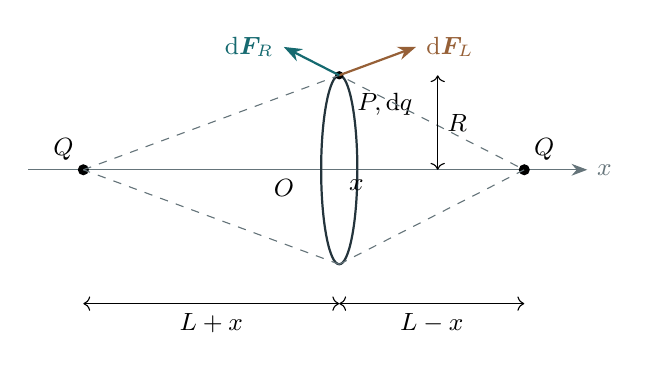
\begin{tikzpicture}[x=1cm,y=1cm,font=\small]
\draw[axis] (-3.5,0)--(3.6,0) node[right] {$x$};
\draw[object] (.45,0) ellipse[x radius=.23,y radius=1.2];
\fill (-2.8,0) circle(2pt) node[above left] {$Q$};
\fill (2.8,0) circle(2pt) node[above right] {$Q$};
\fill (.45,1.2) circle(1.5pt) node[below right=3pt] {$P,\dd q$};
\draw[guide] (-2.8,0)--(.45,1.2)--(2.8,0);
\draw[force] (.45,1.2)--(1.425,1.56) node[right] {$\dd\boldsymbol F_L$};
\draw[motion] (.45,1.2)--(-.255,1.56) node[left] {$\dd\boldsymbol F_R$};
\draw[guide] (.45,-1.2)--(-2.8,0) (.45,-1.2)--(2.8,0);
\node[below left] at (0,0) {$O$};\node[below right] at (.45,0) {$x$};
\draw[<->] (-2.8,-1.7)--(.45,-1.7) node[midway,below] {$L+x$};
\draw[<->] (.45,-1.7)--(2.8,-1.7) node[midway,below] {$L-x$};
\draw[<->] (1.7,0)--(1.7,1.2) node[midway,right] {$R$};
\end{tikzpicture}
\figcaption{解图 电1.14B　环的侧投影及电荷元受力；两斜力的横向分量经全环相加消去。}
\end{minipage}\end{center}

对左点有$\dd F_{Lx}=kQ\dd q(L+x)/d_+^3$，积分即为$kqQ(L+x)/d_+^3$；
右点给负向项。也可先由圆环的轴上场求两个固定点受到的力，再逐项用作用反作用得到环的受力。
在$x=0$两项等大反向，所以平衡存在；受限于轴向平动，求这一方向的位移与合力关系即可判断受限运动。
取无穷远相互作用势为零，环的势能和轴向合力分别为

\begin{align*}
U(x)&=kqQ\left[\frac1{\sqrt{R^2+(L+x)^2}}+\frac1{\sqrt{R^2+(L-x)^2}}\right],\\
F_x(x)&=kqQ\left[\frac{L+x}{[R^2+(L+x)^2]^{3/2}}
-\frac{L-x}{[R^2+(L-x)^2]^{3/2}}\right].
\end{align*}
$F_x(0)=0$。令$f(s)=s(R^2+s^2)^{-3/2}$，则
\[f'(s)=\frac{R^2-2s^2}{(R^2+s^2)^{5/2}},\qquad
F_x=2kqQf'(L)x+O(x^3).
\]
\begin{center}\begin{minipage}{0.97\linewidth}\centering
\begin{tikzpicture}[x=4cm,y=3cm,font=\small]
\draw[axis] (-.78,0)--(1.05,0) node[right] {$\xi=x/R$};
\draw[axis] (0,-.53)--(0,.68) node[above] {$F_x/(kqQ/R^2)$};
\draw[traj,domain=-.65:.65,samples=130] plot(\x,{(1+\x)/(1+(1+\x)^2)^1.5-(1-\x)/(1+(1-\x)^2)^1.5});
\draw[brown,thick,domain=-.65:.65,samples=130] plot(\x,{(.4+\x)/(1+(.4+\x)^2)^1.5-(.4-\x)/(1+(.4-\x)^2)^1.5});
\draw[gray,thick,dashed,domain=-.65:.65,samples=130] plot(\x,{(.70710678+\x)/(1+(.70710678+\x)^2)^1.5-(.70710678-\x)/(1+(.70710678-\x)^2)^1.5});
\node[right,accent] at (.7,.55) {$L/R=1$，稳定};
\node[right,brown] at (.7,.38) {$L/R=.4$，失稳};
\node[right,gray] at (.7,.21) {$L/R=1/\sqrt2$，临界};
\node[below] at (-.65,0) {$-.65$};\node[below] at (.65,0) {$.65$};
\end{tikzpicture}\figcaption{解图 电1.14A　由精确合力计算的三条曲线，临界曲线在原点斜率为零但仍向外推。}\end{minipage}\end{center}
解图电1.14A把原点附近三种力曲线放在同一坐标系中：负斜率对应回复，正斜率对应排斥。临界参数下，原点斜率为零，曲线在正位移处仍为正，左侧反号。下面将求出这条曲线的最低非零项。

所以$L>R/\sqrt2$时力与位移反向，轴向稳定；$L<R/\sqrt2$时力与位移同向，原点不稳定。稳定时回复系数为
\[K=\frac{2kqQ(2L^2-R^2)}{(L^2+R^2)^{5/2}},\]
从$m\ddot x=-Kx$得到
\result{T=2\pi\sqrt{\frac{m(L^2+R^2)^{5/2}}{2kqQ(2L^2-R^2)}}\quad(L>R/\sqrt2).}
这只是振幅趋于零的周期。接近临界值时，一次项很小，使用此式还须把振幅进一步减小。

\subsubsection*{一次回复力怎样产生}
势能为偶函数、力为奇函数，因而原点两侧的判断须互相对称。
由精确式求导可得
\[
F_x'(x)=kqQ\left\{\frac{R^2-2(L+x)^2}{[R^2+(L+x)^2]^{5/2}}
+\frac{R^2-2(L-x)^2}{[R^2+(L-x)^2]^{5/2}}\right\},\qquad
F_x'(0)=-K.
\]
若$U''(0)=K>0$，原点为严格势能极小，充分小的偏移受到回复力；若$K<0$则相反。
$K=0$时一次回复项消失，轴上力的奇对称性使下一阶为三次项，以下用这一项确定偏移后的受力方向。
临界情况将从两个力分式的下一项确定。

也可不先用导数，将$D^2=R^2+L^2$代入两个根式，展开至一次项：
\[
\begin{aligned}
F_x&=\frac{kqQ}{D^3}\left\{(L+x)
 \left[1+\frac{2Lx+x^2}{D^2}\right]^{-3/2}
 -(L-x)\left[1+\frac{-2Lx+x^2}{D^2}\right]^{-3/2}\right\}\\
&\simeq\frac{kqQ}{D^3}\left\{(L+x)\left(1-\frac{3Lx}{D^2}\right)
 -(L-x)\left(1+\frac{3Lx}{D^2}\right)\right\}\\
&\simeq\frac{kqQ}{D^3}\left\{\left(L+x-\frac{3L^2x}{D^2}\right)
 -\left(L-x+\frac{3L^2x}{D^2}\right)\right\}
=-\frac{2kqQ(2L^2-R^2)}{D^5}x.
\end{aligned}
\]
左右两侧的常量抵消，距离变化与轴向投影共同决定一次项的符号。
当$R\to0$且$L>0$，得到$K=4kqQ/L^3$及
$T=2\pi\sqrt{mL^3/(4kqQ)}$，与轴线上两个固定同号点电荷之间的小电荷运动相符。
环半径缩到零时，轴向投影因子趋于1，作用即为两侧库仑排斥力之差。

小振幅条件还可写得更具体。设振幅为$a$，解图电1.14A中的线性回复力与三次项之比要求
\[
a\ll\sqrt{R^2+L^2},\qquad
\frac{|f^{(3)}(L)|a^2}{6|f'(L)|}\ll1.
\]
分母中的 $f'(L)$ 在临界点趋于零。接近临界时，应按第二个不等式进一步缩小振幅，使三次项保持小于一次项。

\Needspace{10\baselineskip}
\subsubsection*{临界点的中间展开}
在$R^2=2L^2$处保留完整的两个分式，先计算力的导数：
\[
\begin{aligned}
F_x'(x)&=-kqQ\left[\frac{4Lx+2x^2}{(3L^2+2Lx+x^2)^{5/2}}
 +\frac{-4Lx+2x^2}{(3L^2-2Lx+x^2)^{5/2}}\right]\\
&=-\frac{2kqQx}{(3L^2)^{5/2}}
\left\{\frac{2L+x}{[1+(2Lx+x^2)/(3L^2)]^{5/2}}
 -\frac{2L-x}{[1+(-2Lx+x^2)/(3L^2)]^{5/2}}\right\}.
\end{aligned}
\]
两个括号相减时常量抵消，因此展开到一次项来取首项。
用$(1+u)^{-5/2}=1-5u/2+35u^2/8+O(u^3)$展开，逐个得到
\[
\begin{aligned}
\frac{2L+x}{[1+(2Lx+x^2)/(3L^2)]^{5/2}}
 &=2L-\frac73x+\frac{5x^2}{9L}+O(x^3/L^2),\\
\frac{2L-x}{[1+(-2Lx+x^2)/(3L^2)]^{5/2}}
 &=2L+\frac73x+\frac{5x^2}{9L}+O(x^3/L^2).
\end{aligned}
\]
所以两者之差为$-14x/3+O(x^3/L^2)$，再次代入有
\[
F_x'(x)=\frac{28kqQ}{27\sqrt3L^5}x^2+O(x^4)>0
\quad(0<|x|\ll L).
\]
在原点两侧力函数均向上增长；再结合$F_x(0)=0$，正侧力为正，负侧力为负。
对该式从0积分，就得到下面直接展开的三次力；再作负积分得到四次势能，所得势能沿两侧向下弯，从另一角度给出相同的运动方向。

在 $R^2=2L^2$ 时，$K=0$ 使三次项成为主导。对$f(L+x)-f(L-x)$保留三次项，
\[F_x=kqQ\left[2f'(L)x+\frac13f^{(3)}(L)x^3+O(x^5)\right]
=\frac{28kqQ}{81\sqrt3L^5}x^3+O(x^5).
\]
三次项仍与位移同向，故临界点不稳定。势能相应为
\[U(x)-U(0)=-\frac{7kqQ}{81\sqrt3L^5}x^4+O(x^6),\]
原点是具有负四次项的平坦势能极大点。
\subsubsection*{势阱的形状与有限振幅}
解图电1.14C直接使用精确势能，取$\ell=L/R,\xi=x/R$，纵坐标为
\[
\frac{U(x)-U(0)}{kqQ/R}=
\frac1{\sqrt{1+(\ell+\xi)^2}}+\frac1{\sqrt{1+(\ell-\xi)^2}}
-\frac2{\sqrt{1+\ell^2}}.
\]
稳定情形在原点向上弯，失稳情形向下弯；临界曲线虽更平，却仍从原点向下。
从临界曲线的原点向两侧走，势能按负四次项下降。

\begin{center}\begin{minipage}{.97\linewidth}\centering
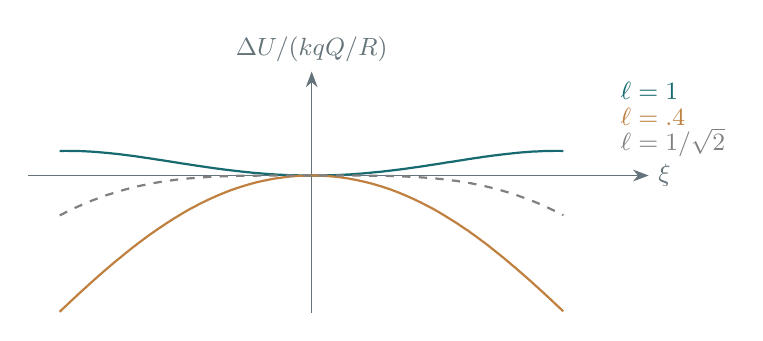
\begin{tikzpicture}[x=4cm,y=6cm,font=\small]
\draw[axis] (-.9,0)--(1.07,0) node[right] {$\xi$};
\draw[axis] (0,-.29)--(0,.22) node[above] {$\Delta U/(kqQ/R)$};
\draw[traj,domain=-.8:.8,samples=160] plot(\x,{1/sqrt(1+(1+\x)^2)+1/sqrt(1+(1-\x)^2)-sqrt(2)});
\draw[brown,thick,domain=-.8:.8,samples=160] plot(\x,{1/sqrt(1+(.4+\x)^2)+1/sqrt(1+(.4-\x)^2)-2/sqrt(1.16)});
\draw[gray,thick,dashed,domain=-.8:.8,samples=160] plot(\x,{1/sqrt(1+(.70710678+\x)^2)+1/sqrt(1+(.70710678-\x)^2)-2/sqrt(1.5)});
\node[right,accent] at (.95,.18) {$\ell=1$};
\node[right,brown] at (.95,.125) {$\ell=.4$};
\node[right,gray] at (.95,.07) {$\ell=1/\sqrt2$};

\end{tikzpicture}
\figcaption{解图 电1.14C　三种精确势能（$|\xi|\le.8$）；临界点是平坦极大点。}
\end{minipage}\end{center}

对于$R>0$的稳定情形，中心只是局部势阱：$U(0)>0$而$U(x)\to0$于无穷远。
正侧刚离开中心时$F_x<0$，在$x=L$却有$F_x=kqQ f(2L)>0$，
故在 $0$ 与 $L$ 之间至少有一个势垒。只有能量低于势垒且初态在中心允许区内，运动才限在中心附近。
解图电1.14D取$L=R$，画出两侧势垒以及低于势垒的能量线；中间相连的允许区域才对应中心往复运动。

\begin{center}\begin{minipage}{.97\linewidth}\centering
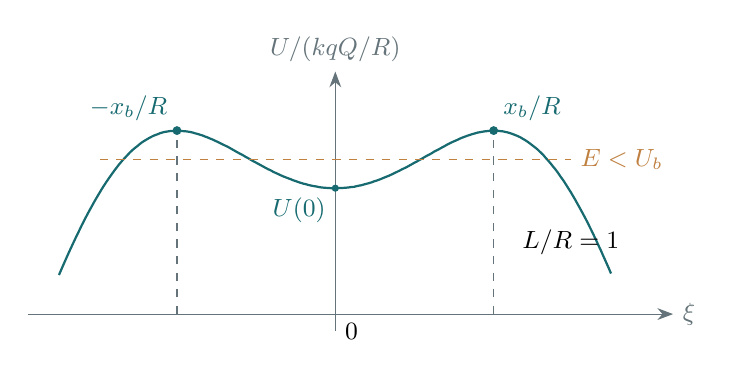
\begin{tikzpicture}[x=2.6cm,y=14cm,font=\small]
\draw[axis] (-1.5,1.3)--(1.65,1.3) node[right] {$\xi$};
\draw[axis] (0,1.285)--(0,1.52) node[above] {$U/(kqQ/R)$};
\draw[traj,domain=-1.35:1.35,samples=220] plot(\x,{1/sqrt(1+(1+\x)^2)+1/sqrt(1+(1-\x)^2)});
\draw[brown,dashed] (-1.15,1.44)--(1.15,1.44) node[right] {$E<U_b$};
\draw[guide] (-.773485,1.3)--(-.773485,1.466454) (.773485,1.3)--(.773485,1.466454);
\fill[accent] (-.773485,1.466454) circle(1.6pt) node[above left] {$-x_b/R$};
\fill[accent] (.773485,1.466454) circle(1.6pt) node[above right] {$x_b/R$};
\fill[accent] (0,1.41421356) circle(1.3pt) node[below left] {$U(0)$};
\node[below right] at (0,1.3) {$0$};\node at (1.15,1.365) {$L/R=1$};
\end{tikzpicture}
\figcaption{解图 电1.14D　有限高度的中心势阱；能量线的中间允许区与外部允许区被势垒隔开。}
\end{minipage}\end{center}

接近临界稳定侧时，记$\kappa=K>0$，并用临界正系数
$c=28kqQ/(81\sqrt3L^5)$表示主阶三次力，则
\[
F_x\simeq-\kappa x+cx^3,\qquad
U(x)-U(0)\simeq\frac{\kappa x^2}2-\frac{cx^4}4.
\]
在临界渐近范围，两侧势垒距中心约为$x_b\simeq\sqrt{\kappa/c}$，
势垒高度约为$\kappa^2/(4c)$，都随$\kappa\to0$缩小。
在这个渐近范围内，简谐近似要求 $a\ll x_b$，此时振幅同时比几何尺度 $R$ 小。
对中心连通区域内的真实转折点$\pm a$，准确周期可由能量积分写成
\[
T(a)=4\sqrt{\frac m2}\int_0^a\frac{\dd x}{\sqrt{U(a)-U(x)}}.
\]
它要求$0<a<x_b$且区间内$U(a)>U(x)$；在充分小振幅极限才化为前面的简谐周期。
到临界参数时，中心已是平坦极大点，受到微扰后向外运动。


\Needspace{18\baselineskip}

\pdfbookmark[2]{第 15 题 带电粒子束的电场聚焦}{q15}

\section*{第 15 题\quad 带电粒子束的电场聚焦}\label{q:15}

质量为$m$、电荷为$q>0$的粒子，从$P_1=(-R,0)$以同一速率$v_0$沿与$+x$轴成$0<\phi<\pi/2$的各方向射出。设计一个电场，使这些粒子都经过$P_2=(R,0)$。忽略重力和粒子间作用。给出场的形式、轨迹与会聚条件；若采用分区匀强场模型，须说明边界及其物理含义。

\begin{center}\begin{minipage}{0.97\linewidth}\centering
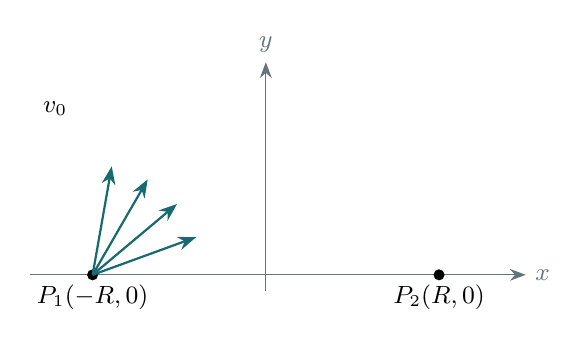
\begin{tikzpicture}[x=1cm,y=1cm]
\draw[axis] (-3,0)--(3.3,0) node[right] {$x$};\draw[axis] (0,-.2)--(0,2.7) node[above] {$y$};
\fill (-2.2,0) circle (2pt) node[below] {$P_1(-R,0)$};\fill (2.2,0) circle (2pt) node[below] {$P_2(R,0)$};
\foreach \a in {20,40,60,80}\draw[motion] (-2.2,0)--++(\a:1.4);\node[above left] at (-2.4,1.9) {$v_0$};
\end{tikzpicture}\figcaption{图 电1.15　同一点以不同仰角射出的等速粒子，要求经过右侧目标点。}\end{minipage}\end{center}

\Needspace{6\baselineskip}\subsection*{解答}

\textbf{一种连续静电场的设计。} 取平面内指向原点的线性场
\[\vect E(x,y)=-\frac{m\omega^2}{q}(x\vect e_x+y\vect e_y),\qquad \omega=\frac{v_0}{R}.\]
它对应电势$\varphi=m\omega^2(x^2+y^2)/(2q)$，两方向的运动方程都是$\ddot x=-\omega^2x,\ddot y=-\omega^2y$。代入初态
$x(0)=-R,y(0)=0,\dot x(0)=v_0\cos\phi,\dot y(0)=v_0\sin\phi$，得
\[x=-R\cos\omega t+R\cos\phi\sin\omega t,\qquad
y=R\sin\phi\sin\omega t.\]
\begin{center}\begin{minipage}{0.97\linewidth}\centering
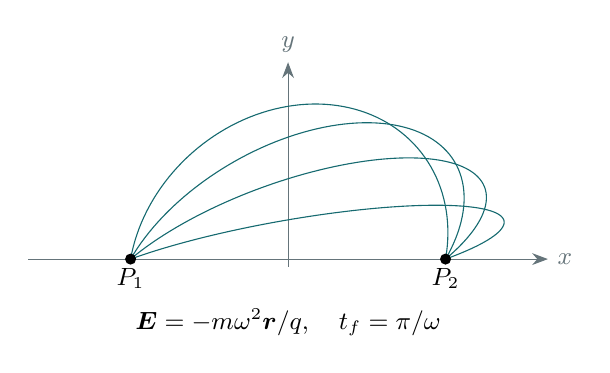
\begin{tikzpicture}[x=1cm,y=1cm]
\draw[axis] (-3.3,0)--(3.3,0) node[right] {$x$};\draw[axis] (0,-.1)--(0,2.5) node[above] {$y$};
\foreach \a in {20,40,60,80}{\draw[accent,domain=0:180,samples=80] plot ({-2*cos(\x)+2*cos(\a)*sin(\x)},{2*sin(\a)*sin(\x)});}
\fill (-2,0) circle (2pt) node[below] {$P_1$};\fill (2,0) circle (2pt) node[below] {$P_2$};\node at (0,-.8) {$\vect E=-m\omega^2\vect r/q,\quad t_f=\pi/\omega$};
\end{tikzpicture}\figcaption{解图 电1.15A　等频线性场中的轨迹：所有速度项在半周期后消失。}\end{minipage}\end{center}
解图电1.15A中各条轨迹的初速度方向不同，而两坐标的振动频率相同；经过半周期时所有含初速度的$\sin\omega t$项一起归零，才在对称点会聚。解图电1.15B则给另一种分区构造，会聚由每一段的进出点和速度共同决定。

\subsubsection*{不同出射方向的共同会聚时刻与会聚速度}
把运动方程写成$\boldsymbol r(t)=\boldsymbol r_0\cos\omega t+
\boldsymbol v(0)\sin\omega t/\omega$，其中$\boldsymbol r_0=-R\boldsymbol e_x$。
任意两个出射方向的轨迹差为
\[
\Delta\boldsymbol r(t)=\frac{\Delta\boldsymbol v(0)}\omega\sin\omega t.
\]
要让不同出射方向的位置差同时归零，取$\sin\omega t=0$；除发射瞬间外，最早共同会聚时刻是$\pi/\omega$。
解图电1.15C把共同的速度响应与位置项画出：前者再次为零时，后者恰把$-R$变成$+R$。

\begin{center}\begin{minipage}{.97\linewidth}\centering
\begin{tikzpicture}[x=5cm,y=1.45cm,font=\small]
\draw[axis] (-.1,0)--(1.4,0) node[right] {$\omega t/\pi$};
\draw[axis] (0,-1.2)--(0,1.4) node[above] {响应系数};
\draw[traj,domain=0:1,samples=100] plot(\x,{sin(180*\x)});
\draw[brown,thick,dashed,domain=0:1,samples=100] plot(\x,{-cos(180*\x)});
\draw[guide] (1,0)--(1,1);\node[below] at (1,0) {$1$};
\node[left] at (0,1) {$1$};\node[left] at (0,-1) {$-1$};
\node[right,accent] at (1.12,.8) {$\sin\omega t$};
\node[right,brown] at (1.12,.4) {$-\cos\omega t$};
\fill[accent] (1,0) circle(1.5pt);\fill[brown] (1,1) circle(1.5pt);
\end{tikzpicture}
\figcaption{解图 电1.15C　半周期时方向相关的速度响应归零，初始位置关于场中心反演。}
\end{minipage}\end{center}

会聚位置由各条轨迹在同一时刻的坐标决定，接近该点的方向由速度给出。
对解图电1.15A的轨迹求导，焦点处
\[
\dot x(t_f)=-v_0\cos\phi,\qquad\dot y(t_f)=-v_0\sin\phi.
\]
所以粒子由右上侧回到$P_2$，速率仍为$v_0$。
两个对称点的势能$q\varphi=m\omega^2(x^2+y^2)/2$相同，机械能守恒也给出相同的速率。

无论$\phi$取何值，在同一时刻$t_f=\pi/\omega=\pi R/v_0$都有$x=R,y=0$，因而
\result{\text{全部粒子在 }t_f=\pi R/v_0\text{ 会聚于 }P_2.}
这一场可在理想的固定、均匀负体电荷长圆柱内部构造。柱内的场为$E_r=\rho_e r/(2\varepsilon_0)$，所需体电荷密度为
\[\rho_e=-\frac{2\varepsilon_0mv_0^2}{qR^2}.\]
轨迹满足
\[x^2+y^2=R^2[1-\cos\phi\sin(2\omega t)]\le2R^2,\]
所以柱半径大于$\sqrt2R$足以包含全部轨迹。这里背景电荷被固定，粒子束足够稀，不改变给定场。

\subsubsection*{场的电荷分布与有效区域}
选半径r、长度h的同轴高斯柱，内部均匀体电荷给
$E_r(2\pi rh)=\rho_e\pi r^2h/\varepsilon_0$，故
$E_r=\rho_e r/(2\varepsilon_0)$，与前面的线性回复场逐项比较便得所列负密度。
该场有$\nabla\times\boldsymbol E=0$，且三维长圆柱模型中$E_z=0$，
$\nabla\cdot\boldsymbol E=\rho_e/\varepsilon_0$；所以两个横向线性回复分量由固定的负体电荷共同产生。
由已给轨迹半径式，$|\cos\phi\sin2\omega t|\le1$，
所以半径大于$\sqrt2R$的柱体足以容纳全部给定轨迹。
单条轨迹的最大半径为$R\sqrt{1+\cos\phi}$，在$\omega t=3\pi/4$处取得。$\phi$越小，这个最大半径越接近$\sqrt2R$。图A中伸到$P_2$右侧的轨迹也说明圆柱须伸出半径$R$的圆。

\textbf{分区匀强力场的轨迹构造。} 还可研究一个理想模型：曲线边界以内场竖直向下，大小$E_0$，边界以外无场。记$a_0=qE_0/m$。粒子沿直线到达左边界$(-X,Y)$后作抛物线运动，由对称性从$(X,Y)$离开，并以与水平线成$-\phi$的方向射向$P_2$。
\begin{center}\begin{minipage}{0.97\linewidth}\centering
\begin{tikzpicture}[x=1cm,y=1cm]
\draw[axis] (-2.5,0)--(2.7,0) node[right] {$x$};\draw[axis] (0,-.1)--(0,2.8) node[above] {$y$};
\foreach \sgn in {-1,1}\draw[object,domain=0:65,samples=70] plot ({\sgn*1.8*sin(\x)*cos(\x)},{1.8*(tan(\x)-sin(\x)^2)});
\draw[traj] (-1.8,0)--(-.9,.9);\draw[traj,domain=0:1.41421356,samples=50] plot ({-.9+1.2727922*\x},{.9+1.2727922*\x-.9*\x^2});\draw[traj] (.9,.9)--(1.8,0);
\fill (-1.8,0) circle (2pt) node[below] {$P_1$};\fill (1.8,0) circle (2pt) node[below] {$P_2$};\node[left] at (-.9,.9) {$(-X,Y)$};\node[right] at (.9,.9) {$(X,Y)$};\draw[force] (.2,2.35)--(.2,1.6) node[right] {$E_0$};
\end{tikzpicture}\figcaption{解图 电1.15B　分区匀强力场的几何构造；图示$\phi=45^\circ$的一条路径，场实现条件另见正文。}\end{minipage}\end{center}
场内水平速度为$v_0\cos\phi$，竖直速度从$v_0\sin\phi$变为其相反数，故场内时间及半宽为
\[\Delta t=\frac{2v_0\sin\phi}{a_0},\qquad
X=\frac{v_0^2\sin\phi\cos\phi}{a_0}.\]
入射直线给出$Y=(R-X)\tan\phi$。取$a_0=v_0^2/R$，便得到一组明确的边界参数式
\[X=R\sin\phi\cos\phi,\qquad Y=R\tan\phi-R\sin^2\phi,
\quad0<\phi<\pi/2.
\]
右边界也可写成$v_0^2Y(R-X)=a_0X[(R-X)^2+Y^2]$，左边界关于$y$轴对称。场内轨迹由
\[x=-X+v_0\cos\phi\,\tau,\qquad
y=Y+v_0\sin\phi\,\tau-\tfrac12a_0\tau^2
\]
给出；在$\tau=\Delta t$时到达右边界，离场后直线斜率为$-\tan\phi$，因而经过$P_2$。

\subsubsection*{半射程与两侧边界的消元}
若整个上半平面都用竖直向下匀强场，从$P_1$出发再次回到水平线的射程是
$v_0^2\sin2\phi/a_0$，随角度变化。两焦点间距固定为$2R$。
分区构造的作用是让粒子在进场前和离场后保留直线段，再选择场内弯折的长度。
图B的$(-X,Y)$和$(X,Y)$等高；场内水平速度不变，竖直速度由正变负，
因而左右等高点关于顶点对称。这既给出前面的全程时间，也可用半程时间$t_h$写成
\[
X=(v_0\cos\phi)t_h,\qquad v_0\sin\phi=a_0t_h,
\qquad\sin\phi\cos\phi=\frac{a_0X}{v_0^2}.
\]
离场直线连接$(X,Y)$与$P_2=(R,0)$，所以
\[
\sin\phi=\frac{Y}{\sqrt{Y^2+(R-X)^2}},\qquad
\cos\phi=\frac{R-X}{\sqrt{Y^2+(R-X)^2}}.
\]
相乘并代入半射程关系，得到右半边界
\[
v_0^2y(R-x)=a_0x[(R-x)^2+y^2],\qquad x\ge0.
\]
交界线取参数式中$0<\phi<\pi/2$的正高分支。
反射$x\mapsto-x$得到左半边界
\[
v_0^2y(R+x)=-a_0x[(R+x)^2+y^2],\qquad x\le0.
\]
对正文选定的$a_0=v_0^2/R$，有$0<X\le R/2$且$Y>0$；
当$\phi\downarrow0$，边界趋向O，当$\phi\uparrow\pi/2$，$Y\to\infty$。
当$\phi\to\pi/2$时，$Y(\phi)=R\tan\phi-R\sin^2\phi$趋于无穷。图B截取其中一段，较陡的入射轨迹在更高处进入力场区。
图B中各高度只对应一对交界点。由参数式，$Y'(\phi)=R(\sec^2\phi-\sin2\phi)>0$，因此给定高度$y>0$能反推出交界点的参数$\psi$，其半宽为$R-y/\tan\psi$。在场内的右半段，消去$\tau$得
\[
y=Y+\frac{\tan\phi}{2X}(X^2-x^2),\qquad 0\le x\le X.
\]
此段的$y$至少为$Y$，所以$\psi\ge\phi$。把抛物线与通向$P_2$的直线延长段比较，$(R-x)\tan\phi-y=\tan\phi\,(X-x)^2/(2X)$；随即有$R-y/\tan\psi\ge R-y/\tan\phi\ge x$。因此抛物线确在有场区域内，且在$x=X$处接到交界线。离场后的直线上$y<Y$、$\psi<\phi$，其横坐标$x=R-y/\tan\phi$大于该高度的场区半宽。左侧由对称性得到同样关系。跨过交界线时场力有界，过面时段趋零，冲量也趋零，故速度连续。

两种构造在场的性质上不同。线性场由电势给出，分区力场的环流则可从交界线两侧直接算出。
\subsubsection*{场区交界处的切向电场与环流}
解图电1.15D取交界线上有高度差的一段，在其两侧各取一条平行长边，首尾用很短的边连接。
沿场内长边向上走，积分为$-E_0\Delta y$；沿场外长边返回，积分为零。
令两短边间距趋零，其贡献也趋零，仍留下
\[
\oint\boldsymbol E\cdot\dd\boldsymbol l=-E_0\Delta y\ne0.
\]
静电场的闭合环流为零，因此交界线两侧的切向电场须连续。普通表面电荷产生的是法向分量的跳变；图D中的非零环流来自切向分量的差值。

\begin{center}\begin{minipage}{.97\linewidth}\centering
\begin{tikzpicture}[x=1.4cm,y=1.4cm,font=\small]
\draw[object] (-.9,-1.2)--(.9,1.2) node[above] {局部边界};
\draw[->,accent,thick] (-.76,-.43)--(.2,.85)--(.76,.43)--(-.2,-.85)--cycle;
\draw[force] (-1.2,.6)--(-1.2,-.1) node[midway,left] {$\boldsymbol E=-E_0\boldsymbol e_y$};
\node[right] at (1.15,-.3) {$\boldsymbol E=0$};
\node[below] at (0,-1.2) {两长边平行，短边宽度趋于零};
\end{tikzpicture}
\figcaption{解图 电1.15D　跨过非水平交界线的小环路，场内长边给出非零切向积分。}
\end{minipage}\end{center}

在指定分段力场的几何聚焦模型中，粒子沿前面求出的分区抛物线运动。若要求电场由静止电荷产生，可用前面的连续线性场及其固定负电荷背景；粒子的轨迹由该场对应的运动方程给出。


\Needspace{18\baselineskip}

\pdfbookmark[2]{第 16 题 两个半球面的底面电势}{q16}

\section*{第 16 题\quad 两个半球面的底面电势}\label{q:16}

两个均匀带电的薄半球面具有同一球心和同一底面平面，分处该平面的两侧，半径为$R_1>R_2$，面电荷密度分别为$\sigma_1,\sigma_2$。求较大半球底面的一条直径$AOB$上各点的电势，取无穷远电势为零。

\begin{center}\begin{minipage}{0.97\linewidth}\centering
\begin{tikzpicture}[x=1cm,y=1cm]
\draw[axis] (-3,0)--(3.2,0) node[right] {$x$};\draw[object] (2.4,0) arc (0:180:2.4);\draw[object] (-1.3,0) arc (180:360:1.3);
\node[above] at (0,2.4) {$R_1,\sigma_1$};\node[below] at (0,-1.3) {$R_2,\sigma_2$};\node[below] at (-2.4,0) {$A$};\node[below] at (2.4,0) {$B$};\node[below left] at (0,0) {$O$};\fill (.75,0) circle (2pt) node[above] {$P$};
\end{tikzpicture}\figcaption{图 电1.16　沿共同底面的直径观察，两个半球分居底面的两侧。}\end{minipage}\end{center}

\Needspace{6\baselineskip}\subsection*{解答}

令观察点到共同球心的距离为$r=|x|$。取共同底面为$z=0$。在任意一个半球上取面元$(X,Y,Z)$，在另一侧补上镜像面元$(X,Y,-Z)$。
\begin{center}\begin{minipage}{0.97\linewidth}\centering
\begin{tikzpicture}[x=1cm,y=1cm]
\draw[object] (0,0) circle (1.65);\draw[guide] (-2.2,0)--(2.2,0);\coordinate (P) at (.6,0);\coordinate (A) at (120:1.65);\coordinate (B) at (240:1.65);\draw[accent] (A)--(P)--(B);\fill (P) circle (2pt) node[right] {$P$};\fill[accent] (A) circle (2pt) node[above] {$\dd q$};\fill[muted] (B) circle (2pt) node[below] {镜像$\dd q$};\node[right,align=left] at (2.6,.2) {两距离相同\\半球势为完整球面的一半};
\end{tikzpicture}\figcaption{解图 电1.16A　补全一个半球；底面点到一对镜像电荷元等距。}\end{minipage}\end{center}
解图电1.16A中，底面点$P=(x,0,0)$到两个镜像面元的距离平方同为$(x-X)^2+Y^2+Z^2$。每对面元的势相等，逐对加起来，补成的完整球面的势就是实际半球面电势的两倍。

半径$R_i$、面密度$\sigma_i$的完整球面总电荷为$4\pi R_i^2\sigma_i$。由球壳定理，它在$r\le R_i$和$r>R_i$的电势分别为$4\pi k\sigma_iR_i$和$4\pi k\sigma_iR_i^2/r$。所以半球面在底面内的电势为
\[\varphi_i(r)=\frac{\sigma_iR_i^2}{2\varepsilon_0\max(R_i,r)}.\]
\subsubsection*{先求完整球面，再分成两个等势贡献}
设补全后的总电量为$Q_i^{\rm full}=4\pi R_i^2\sigma_i$，
而实际半球只有$q_i^{\rm hemi}=2\pi R_i^2\sigma_i$。
对完整球面，高斯定律给球内$E_r=0$、球外$E_r=kQ_i^{\rm full}/r^2$；
以无穷远为势零点，积分得到
\[
\varphi_i^{\rm full}(r)=\begin{cases}
kQ_i^{\rm full}/R_i,&r\le R_i,\\
kQ_i^{\rm full}/r,&r>R_i.
\end{cases}
\]
从无穷远积分到球面得到$kQ_i^{\rm full}/R_i$。继续向内时场为零，电势维持球面处的值。
图A的镜像配对把面积元、电荷和到P的距离逐一保留，
故$\varphi_i^{\rm hemi}(P)=\varphi_i^{\rm full}(P)/2$。
若$\sigma_i$为负，一对镜像元的电势贡献同为负值。

大球在$0\le r\le R_1$上的计算依次为
\[
\varphi_1^{\rm full}=\frac{4\pi R_1^2\sigma_1}{4\pi\varepsilon_0R_1}
=\frac{\sigma_1R_1}{\varepsilon_0},\qquad
\varphi_1^{\rm hemi}=\frac{\sigma_1R_1}{2\varepsilon_0}.
\]
小球则须先按$r\le R_2$与$r>R_2$分开：
\[
\begin{aligned}
\varphi_2^{\rm full}(r)&=\begin{cases}
\sigma_2R_2/\varepsilon_0,&r\le R_2,\\
\sigma_2R_2^2/(\varepsilon_0r),&r>R_2,
\end{cases}\\
\varphi_2^{\rm hemi}(r)&=\frac12\varphi_2^{\rm full}(r).
\end{aligned}
\]
把两个半球的贡献相加得到共同底面的电势。

较大半球在整段$AB$上都贡献常量$\sigma_1R_1/(2\varepsilon_0)$；较小半球须分区。因此
\result{\varphi(x)=\begin{cases}
\dfrac{\sigma_1R_1+\sigma_2R_2}{2\varepsilon_0},&|x|\le R_2,\\[4pt]
\dfrac{\sigma_1R_1}{2\varepsilon_0}+\dfrac{\sigma_2R_2^2}{2\varepsilon_0|x|},&R_2<|x|\le R_1.
\end{cases}}
两式在$|x|=R_2$连续，在$O$也没有奇点。中央底面上的切向电场为零，法向场由两片半球产生的法向分量叠加。
\subsubsection*{分区、连续性与切向场}
在$x=\pm R_2$，外段的$\sigma_2R_2^2/|x|$都回到$\sigma_2R_2$，
两支电势严格相接；在球心使用内段常数。
解图电1.16B选$R_1=2R_2,\sigma_1=\sigma_2=\sigma_0>0$，
用$\xi=x/R_2$与$\widehat\varphi=2\varepsilon_0\varphi/(\sigma_0R_2)$表示实际函数：
中段为3，外侧为$2+1/|\xi|$，两端为$5/2$。
图B在$\xi=\pm1$处从常势段转入反比段。

\begin{center}\begin{minipage}{.97\linewidth}\centering
\begin{tikzpicture}[x=1.8cm,y=1.3cm,font=\small]
\draw[axis] (-2.4,2.15)--(2.55,2.15) node[right] {$\xi$};
\draw[axis] (0,2.1)--(0,3.5) node[above] {$\widehat\varphi$};
\draw[traj] (-1,3)--(1,3);
\draw[traj,domain=-2:-1,samples=70] plot(\x,{2-1/\x});
\draw[traj,domain=1:2,samples=70] plot(\x,{2+1/\x});
\foreach \x in {-2,-1,1,2}{\draw[guide] (\x,2.15)--(\x,{2+1/max(1,abs(\x))});\node[below] at (\x,2.15) {$\x$};}
\node[above left] at (0,3) {$3$};\node[left] at (0,2.5) {$5/2$};
\node at (1.5,3.32) {$R_1=2R_2$};
\end{tikzpicture}
\figcaption{解图 电1.16B　正等面密度的一例：中央常势段与两侧反比变化段连续相接。}
\end{minipage}\end{center}

沿直径求导可得不在边缘处的切向分量
\[
E_x(x)=\begin{cases}
0,&|x|<R_2,\\
\dfrac{\sigma_2R_2^2}{2\varepsilon_0}\dfrac{x}{|x|^3},&R_2<|x|<R_1.
\end{cases}
\]
由$\dd |x|/\dd x=\operatorname{sgn}x$，正、负两侧的$E_x$方向相反。到小半球边缘的内侧极限为零，外侧极限在$+R_2$处为$\sigma_2/(2\varepsilon_0)$、在$-R_2$处为$-\sigma_2/(2\varepsilon_0)$。两侧的电势相接，切向电场的单侧极限有差值。

\subsubsection*{两半球在球心的法向电场}
另求球心的法向分量。取底面为$z=0$，大半球在上、小半球在下。
解图电1.16C以正面密度为例，画出两半球在O的相反法向场；半球半径在面积元和距离平方因子中相消。
对上半球，以正z为极轴，$\dd S=2\pi R_1^2\sin\theta\dd\theta$，有
\[
E_{1z}(O)=-2\pi k\sigma_1\int_0^{\pi/2}\cos\theta\sin\theta\dd\theta
=-\pi k\sigma_1=-\frac{\sigma_1}{4\varepsilon_0}.
\]
下半球贡献为$E_{2z}(O)=\sigma_2/(4\varepsilon_0)$，因此
\[
E_z(O)=\frac{\sigma_2-\sigma_1}{4\varepsilon_0}.
\]
图C中下半球的面密度较大，合场向上。沿底面求导得到切向场，沿$z$方向的场这里由电荷积分直接给出。在图A补全一个半球时，一对镜像元的法向场方向相反，大小相等，因而补出的部分恰抵消该半球的法向场。

\begin{center}\begin{minipage}{.97\linewidth}\centering
\begin{tikzpicture}[x=1cm,y=1cm,font=\small]
\draw[axis] (-2.8,0)--(3,0) node[right] {$x$};
\draw[axis] (0,-1.6)--(0,2.6) node[above] {$z$};
\draw[object] (2.4,0) arc(0:180:2.4);
\draw[object] (-1.2,0) arc(180:360:1.2);
\draw[force] (0,0)--(0,-.55) node[right] {$\boldsymbol E_1$};
\draw[motion] (0,0)--(0,1.1) node[right] {$\boldsymbol E_2$};
\fill (0,0) circle(1.5pt) node[below left] {$O$};
\node at (-1.4,1.35) {$\sigma_1>0$};\node at (-1.7,-.85) {$\sigma_2=2\sigma_1$};
\end{tikzpicture}
\figcaption{解图 电1.16C　两半球在球心的法向场；图取$\sigma_2=2\sigma_1>0$，合场向上。}
\end{minipage}\end{center}


\Needspace{18\baselineskip}

\pdfbookmark[2]{第 17 题 带电圆环电势的球面平均}{q17}

\section*{第 17 题\quad 带电圆环电势的球面平均}\label{q:17}

半径$R_1$、总电荷$Q$的细圆环，其轴线上有一半径$R_2$的球面，球心到环心距离为$L$。求圆环电荷在该球面上产生的电势的面积平均值。球面只是取平均的几何曲面，不是导体；取无穷远电势为零，并讨论球面包围圆环与不包围圆环的情形。

\begin{center}\begin{minipage}{0.97\linewidth}\centering
\begin{tikzpicture}[x=1cm,y=1cm]
\draw[object] (-2,0) ellipse (.35 and 1.2);\draw[object] (1.5,0) circle (1.5);\draw[guide] (-2.6,0)--(3.5,0);\fill (-2,0) circle (1pt) node[below] {$O$};\fill (1.5,0) circle (1pt) node[below] {$C$};\draw[<->] (-2,-1.8)--(1.5,-1.8) node[midway,below] {$L$};\node[above] at (-2,1.2) {圆环$Q,R_1$};\draw (1.5,0)--++(45:1.5) node[midway,left] {$R_2$};
\end{tikzpicture}\figcaption{图 电1.17　球面用于取面积平均；图示为圆环位于球面外的一种位置。}\end{minipage}\end{center}

\Needspace{6\baselineskip}\subsection*{解答}

圆环上每一点到球心$C$的距离都为$r_0=\sqrt{R_1^2+L^2}$。要求的是电势的面积平均
\[\overline\varphi=\frac1{4\pi R_2^2}\int_{S_2}\varphi_{\rm ring}\,\dd S.\]
\subsubsection*{球面平均中的旋转对称性}
在环上取等量元$\dd q$，将它绕轴从一个位置转到另一个位置，
同时把整个积分球面作同一刚体转动。球面作为点集及其面积元都不变，
每一对源点与观察点的距离保持，所以该电荷元的球面平均贡献不变。
每个环元因此带有同一个单位电荷平均系数。把各元的贡献相加等价于先求环上一个点电荷$Q$的球面平均，环上的电荷密度可以随位置变化。
若直接积分，可以以该点电荷与C的连线作极轴，把球面分成等势的纬圈，
每圈的权重正比于该圈的面积。它们自然出现在后面的角积分中。


在这个几何球面上引入辅助的均匀面电荷，总量取$Q_s$。它和圆环的相互作用能可按任一电荷分布来积分。
\begin{center}\begin{minipage}{0.97\linewidth}\centering
\begin{tikzpicture}[x=1cm,y=1cm]
\draw[accent,dashed] (1.2,0) circle (1.45);\draw[object] (-2,0) ellipse (.25 and 1.05);\draw[guide] (-2,1.05)--(1.2,0)--(-2,-1.05);\node[above] at (-.5,.65) {$r_0$};\fill (1.2,0) circle (1pt) node[right] {$C$};\node[above] at (1.2,1.5) {辅助均匀球面$Q_s$};\node at (.1,-2) {$Q_s\overline\varphi=\int_{\rm ring}\varphi_s\dd q$};
\end{tikzpicture}\figcaption{解图 电1.17A　交换相互作用能的积分顺序；环上各点到C的距离相同。}\end{minipage}\end{center}
解图电1.17A中，将辅助均匀球面置于待平均的几何球面上，总电荷取$Q_s$。按球面积分的相互作用能是$Q_s\overline\varphi$；改按圆环积分时，环上各元到$C$等距，辅助球势在环上为同一值。令两个积分相等，就可用辅助球壳在环上的势来求球面平均。

\subsubsection*{相互作用能的两种等价算法}
先看相距d的两个点电荷$Q_1,Q_2$：
$Q_1\varphi_2=Q_2\varphi_1=kQ_1Q_2/d$。
两种记法计算的是同一对电荷的一份相互作用能。
推广到两个给定分布，每一对电荷元的相互作用为
$k\dd q\dd Q_s/|\boldsymbol r-\boldsymbol R|$，因此
\[
\begin{aligned}
W_{\rm int}
&=k\int_{\rm ring}\int_{S_2}
 \frac{\dd q\dd Q_s}{|\boldsymbol r-\boldsymbol R|}\\
&=\int_{S_2}\varphi_{\rm ring}\dd Q_s
=\int_{\rm ring}\varphi_s\dd q.
\end{aligned}
\]
先固定环上的元还是先固定球面上的元，只改变积分顺序。
若从$\tfrac12\int\rho\varphi$的总场能表达式出发，
两个交叉项各出现一次，前面的二分之一把两份相等的交叉积分合成一份相互作用能。

选辅助球面均匀，正是为了使$\dd Q_s=Q_s\dd S/(4\pi R_2^2)$。
取任意非零$Q_s$后，按球面积分的一端等于$Q_s$乘待求面积平均；
按环积分的一端则利用已知球壳内、外电势。
这里的$\dd Q_s$是积分权重，最后约去$Q_s$就还原成圆环电势的面积平均。若改用随位置变化的辅助密度，相同方法得到的是密度加权的平均。


先在球面上积分，有
\[W_{\rm int}=\int_{S_2}\varphi_{\rm ring}\frac{Q_s}{4\pi R_2^2}\dd S
=Q_s\overline\varphi.\]
再对圆环电荷积分。辅助球面在所有环上点的电势相同，为$kQ_s/\max(R_2,r_0)$，于是
\[W_{\rm int}=\int_{\rm ring}\frac{kQ_s}{\max(R_2,r_0)}\dd q
=\frac{kQ_sQ}{\max(R_2,r_0)}.\]
两式相等，约去$Q_s$，得到
\result{\overline\varphi=\begin{cases}
\dfrac{kQ}{\sqrt{R_1^2+L^2}},&R_2\le\sqrt{R_1^2+L^2},\\[4pt]
\dfrac{kQ}{R_2},&R_2\ge\sqrt{R_1^2+L^2}.
\end{cases}}
在$R_2<r_0$一支，球内没有环上电荷，平均值等于球心电势。在$R_2>r_0$一支，圆环全处在球内，球面平均按$1/R_2$变化。

\subsubsection*{内外两支及平均值随球半径的变化}
解图电1.17B分别画出半径小于和大于$r_0$的球面。环上所有元的距离都是$r_0$，
因此球面半径小于$r_0$时全部元在辅助球壳外，
球面半径大于$r_0$时全部元在其内。若$R_2=r_0$，所有环元都在球面上。

\begin{center}\begin{minipage}{.97\linewidth}\centering
\begin{tikzpicture}[x=1cm,y=1cm,font=\small]
\begin{scope}[xshift=-2.9cm]
\draw[accent,dashed] (0,0) circle(1.15);
\draw[guide] (-.95,-1.2)--(-.95,1.2);
\draw[guide] (0,0)--(-.95,1.2);
\fill (0,0) circle(1.2pt) node[right] {$C$};
\fill (-.95,1.2) circle(1.4pt) node[above left] {环元};
\fill (-.95,-1.2) circle(1.4pt);
\node[above right] at (-.5,.6) {$r_0$};
\node at (0,2.45) {$R_2<r_0$};
\node at (0,-2.45) {环在球面外，使用外势};
\end{scope}
\begin{scope}[xshift=2.9cm]
\draw[accent,dashed] (0,0) circle(2.1);
\draw[guide] (-.95,-1.2)--(-.95,1.2);
\draw[guide] (0,0)--(-.95,1.2);
\fill (0,0) circle(1.2pt) node[right] {$C$};
\fill (-.95,1.2) circle(1.4pt) node[above left] {环元};
\fill (-.95,-1.2) circle(1.4pt);
\node[above right] at (-.5,.6) {$r_0$};
\node at (0,2.45) {$R_2>r_0$};
\node at (0,-2.45) {环被球面包围，使用内势};
\end{scope}
\end{tikzpicture}
\figcaption{解图 电1.17B　实点是圆环在轴截面上的交点，虚线沿环所在平面。}
\end{minipage}\end{center}

在图B左侧，增大球面时仍使用同一个外势$kQ_s/r_0$，平均值维持不变。到了右侧，使用球壳内势$kQ_s/R_2$，所以平均值随球半径衰减。
解图电1.17C取$Q>0$，以$\xi=R_2/r_0$为横轴，画出归一平均值，
在$\xi=1$连续，而斜率的两侧极限不同。

\begin{center}\begin{minipage}{.97\linewidth}\centering
\begin{tikzpicture}[x=2.4cm,y=2cm,font=\small]
\draw[axis] (0,0)--(2.9,0) node[right] {$\xi=R_2/r_0$};
\draw[axis] (0,0)--(0,1.45) node[above] {$\overline\varphi/(kQ/r_0)$};
\draw[traj] (0,1)--(1,1);
\draw[traj,domain=1:2.6,samples=100] plot(\x,{1/\x});
\draw[guide] (1,0)--(1,1);\fill[accent] (1,1) circle(1.5pt);
\node[left] at (0,1) {$1$};\node[below] at (1,0) {$1$};
\node[below] at (2,0) {$2$};\node at (.5,1.23) {常值};
\node at (1.9,.86) {$1/\xi$};
\end{tikzpicture}
\figcaption{解图 电1.17C　面积平均随球面半径的精确两支函数，半径零点只表示极限。}
\end{minipage}\end{center}


为求球面恰好经过圆环时的面积权重，把一个环元视作点电荷$q'$，令它到球心的距离为$s$，以从球心指向它的方向为极轴。积分写成
\begin{align*}
\frac1{4\pi}\int\frac{kq'\dd\Omega}{\sqrt{s^2+R_2^2-2sR_2\cos\theta}}
&=\frac{kq'}2\int_{-1}^1\frac{\dd u}{\sqrt{s^2+R_2^2-2sR_2u}}\\
&=\frac{kq'}{2sR_2}\bigl[s+R_2-|s-R_2|\bigr]
=\frac{kq'}{\max(s,R_2)}.
\end{align*}
把$u=1$代入距离根式，得到球面上最近点到源的距离$|s-R_2|$。这个绝对值把源在球内和球外两种情形连在一起。
\subsubsection*{球面经过电荷时的面积积分}
若点电荷恰位于球心，即$s=0$，球面各点到它都为$R_2$，平均直接等于$kq'/R_2$；
含s分母的中间式取同一连续极限。直接积分中的面积元是$\dd S=R_2^2\sin\theta\dd\theta\dd\psi$，
方位角先积分给$2\pi$，再令$u=\cos\theta$，才得到前面的二分之一权重。
积分末端的距离分别为$s+R_2$和$|s-R_2|$，
当源点在球内，较短距离为 $R_2-s$。当源点在球外，较短距离为 $s-R_2$。

当$s=R_2$，点电荷位于积分球面上，邻近该点的距离约为$R_2\theta$，
势核按$1/\theta$增长，而面积权重按$\theta\dd\theta$缩小，
二者乘积仍可积。若细环的线密度在该点连续且非零，把邻近环元沿线积分时，局部势呈对数型变化。
因此两支在$R_2=r_0$接到同一有限值$kQ/r_0$。从单个环元来看，把$\theta<\epsilon$的小球冠单独积分。近极点的距离平方为$(s-R_2)^2+2sR_2(1-\cos\theta)$。在$s$靠近$R_2$时，分母至少和$R_2\theta$同阶，而球冠的面积权重是$R_2^2\sin\theta\,\dd\theta\,\dd\psi$，因此球冠的贡献随$\epsilon$线性减小。其余部分可以直接取$s\to R_2$。


\Needspace{18\baselineskip}

\pdfbookmark[2]{第 18 题 重力与电力共同作用下的最大速度}{q18}

\section*{第 18 题\quad 重力与电力共同作用下的最大速度}\label{q:18}

地面上固定点电荷$Q$。一个质量为$m$的小带电质点沿经过$Q$的竖直线运动，在距地面$H/2$和$H$的两位置之间往复运动。只计重力与库仑力。求质点运动中的最大速度及达到最大速度的位置。

\begin{center}\begin{minipage}{0.97\linewidth}\centering
\begin{tikzpicture}[x=1cm,y=1cm]
\draw[object] (-1.5,0)--(1.8,0);\draw[guide] (0,0)--(0,3.2);\fill (0,0) circle (3pt) node[below] {$Q$};\fill[accent] (0,1.6) circle (3pt) node[left] {$m,q$};\draw[<->] (1,0)--(1,1.2) node[midway,right] {$H/2$};\draw[<->] (1.8,0)--(1.8,2.4) node[midway,right] {$H$};\draw[guide] (-.5,1.2)--(1.1,1.2) (-.5,2.4)--(1.9,2.4);
\end{tikzpicture}\figcaption{图 电1.18　两个转向高度分别为H/2和H；小球只作竖直运动。}\end{minipage}\end{center}

\Needspace{6\baselineskip}\subsection*{解答}

设小质点电荷为$q$，离地高度为$h>0$。它在上下两处都能回转，电力须向上，因而$Qq>0$。记$K=kQq$，取重力势能零点在地面，势能为
\[U(h)=mgh+\frac Kh.\]
在$h=H/2$和$h=H$处速度都为零，能量相等，故
\[\frac12mgH+\frac{2K}{H}=mgH+\frac KH,
\qquad K=\frac12mgH^2.\]
\begin{center}\begin{minipage}{0.97\linewidth}\centering
\begin{tikzpicture}[x=5cm,y=4.8cm,font=\small]
\draw[axis] (.27,1.25)--(1.4,1.25) node[right] {$\eta=h/H$};
\draw[axis] (.27,1.23)--(.27,2.04) node[above] {$u=U/(mgH)$};
\draw[traj,domain=.3:1.25,samples=140] plot(\x,{\x+.5/\x});
\draw[guide] (.5,1.25)--(.5,1.5)--(1,1.5)--(1,1.25);
\draw[guide] (.70710678,1.25)--(.70710678,1.41421356);
\node[below] at (.5,1.25) {$1/2$};\node[below] at (1,1.25) {$1$};
\node[below=14pt] at (.70710678,1.25) {$1/\sqrt2$};
\node[left] at (.27,1.5) {$3/2$};\node[left] at (.27,1.41421356) {$\sqrt2$};
\node[left] at (.27,1.25) {$5/4$};
\draw[guide] (1,1.5)--(1.27,1.5);
\node[right] at (1.3,1.5) {$\mathcal H/(mgH)=3/2$};
\draw[<->] (.70710678,1.41421356)--(.70710678,1.5);
\end{tikzpicture}\figcaption{解图 电1.18A　势能曲线与总能量线，竖直间距乘上$mgH$给出动能。}\end{minipage}\end{center}
\subsubsection*{两个转向点怎样确定未知电力}
在低处要从下降转为上升，合力要向上。所以电力是斥力，而且在低端大于重力。上下两端的动能都为零，用两处势能相等就能确定$K/m$。
将前面的端点等能式整理为
\[
\frac{mgH}{2}=\frac KH,\qquad
\mathcal H=mgH+\frac KH=\frac32mgH.
\]
式中的$K/h=q(kQ/h)$是质点在固定电荷的电势中的势能，与$mgh$具有同一量纲。

任意高度的速率由能量式决定：
\[\frac12mv^2=mgH+\frac KH-mgh-\frac Kh
=mg\left(\frac{3H}{2}-h-\frac{H^2}{2h}\right).
\]
将解图电1.18A对应的动能因式分解：
\[\frac12mv^2=mg\frac{(h-H/2)(H-h)}h.\]
$h>0$时，非负动能恰给$H/2\le h\le H$。在图A上，这一段正是水平能量线位于势能曲线上方的区间，纵坐标以$mgH$为单位，两线的竖直间距乘$mgH$就是动能。

\subsubsection*{力的符号与最大速率的位置}
取向上为正，合力与其导数为
\[
F_h=\frac K{h^2}-mg,\qquad F_h'=-\frac{2K}{h^3}<0.
\]
在下端$H/2$，电力为$2mg$，合力向上。在上端$H$，电力为$mg/2$，合力向下。解图电1.18C按同一尺度画出三个高度的电力和重力，在$H/\sqrt2$处两箭头等长。

\begin{center}\begin{minipage}{.97\linewidth}\centering
\begin{tikzpicture}[x=1cm,y=.8cm,font=\small]
\foreach \X/\a/\lab in {-2.7/2/{H/2},0/1/{H/\sqrt2},2.7/.5/{H}}{
\begin{scope}[xshift=\X cm]
\fill (0,0) circle(2pt) node[left] {$B$};
\draw[motion] (0,0)--(0,\a) node[right] {$F_E$};
\draw[force] (0,0)--(0,-1) node[right] {$mg$};
\node[above] at (0,2.55) {$h=\lab$};
\end{scope}}
\end{tikzpicture}
\figcaption{解图 电1.18C　各高度的局部受力比较，电力依次为重力的2倍、1倍、1/2倍。}
\end{minipage}\end{center}

因为$F_h$随高度严格递减，它只有一个零点。
上行时先在低处加速，过零点后减速。下行时先在高处加速，过零点后减速。两程都在同一高度达到最大速率。从能量式对高度求导也得$\dd v^2/\dd h=2F_h/m$，因而速率平方在合力变号处取极大。

速率在势能最低时最大。令$U'(h)=mg-K/h^2=0$，得到$h_*=H/\sqrt2$；它确在两转向点之间，且$U''=2K/h^3>0$。代入上式，
\result{v_{\max}=\sqrt{(3-2\sqrt2)gH},\qquad h_*=\frac H{\sqrt2}.}
图A中，势谷底的位置$h_*=\sqrt{(H/2)H}$是两个转向高度的几何平均。水平线到谷底的竖直距离给最大动能。
\subsubsection*{势能下界与速率曲线}
势能曲线的最低值也可直接由两项势能的算术—几何平均不等式读出。
\[
U(h)=mgh+\frac Kh\ge2\sqrt{mgK}=\sqrt2mgH,
\]
等号要求$mgh=K/h$，仍给$h=H/\sqrt2$。
因此最大动能和速率平方依次为
\[
\frac12mv_{\max}^2=\mathcal H-U_{\min}
=mgH\left(\frac32-\sqrt2\right),\qquad
v_{\max}^2=(3-2\sqrt2)gH.
\]
若从最低点静止释放，初始机械能为$U_{\min}$，质点停在平衡处。本题的机械能是图A中更高的水平线，所以经过同一位置时动能为正。

解图电1.18B直接画出$\eta=h/H$与$w=v^2/(gH)$的精确关系
$w=3-2\eta-1/\eta$。两端为零，峰顶在$\eta=1/\sqrt2$。同一高度的两次经过分别取$+v$和$-v$，在图B上对应同一个$v^2$。

\begin{center}\begin{minipage}{.97\linewidth}\centering
\begin{tikzpicture}[x=6cm,y=8cm,font=\small]
\draw[axis] (.4,0)--(1.22,0) node[right] {$\eta=h/H$};
\draw[axis] (.4,0)--(.4,.25) node[above] {$v^2/(gH)$};
\draw[traj,domain=.5:1,samples=120] plot(\x,{3-2*\x-1/\x});
\draw[guide] (.70710678,0)--(.70710678,.17157288)--(.4,.17157288);
\fill[accent] (.70710678,.17157288) circle(1.5pt);
\node[below] at (.5,0) {$1/2$};\node[below] at (1,0) {$1$};
\node[below=14pt] at (.70710678,0) {$1/\sqrt2$};
\node[left] at (.4,.17157288) {$3-2\sqrt2$};
\end{tikzpicture}
\figcaption{解图 电1.18B　速率平方的精确函数；最大值出现在两转向高度的几何平均。}
\end{minipage}\end{center}

由$3-2\sqrt2=(\sqrt2-1)^2$，可把峰顶速率写成$(\sqrt2-1)\sqrt{gH}$。保持电荷和质量不变时，改变机械能相当于上下移动图A中的水平线。两个交点随之移动，其高度乘积仍由$K/(mg)$决定。


\Needspace{18\baselineskip}

\pdfbookmark[2]{第 19 题 穿越两个带电球壳的能量门槛}{q19}

\section*{第 19 题\quad 穿越两个带电球壳的能量门槛}\label{q:19}

两个固定的均匀带电球壳，球心为$A,B$，电荷分别为$4Q,Q$，$Q>0$，两球心距离$d$远大于各球壳半径。沿$AB$连线在两球壳上开三个小孔，如图。质量$m$、电荷$-q$（$q>0$）的质点在$A$左侧距$A$为$x$处静止释放。求它穿过三孔并到达$B$球心所需的临界起始距离，说明等于临界值时的运动。忽略小孔对给定均匀电荷分布的影响。

\begin{center}\begin{minipage}{0.97\linewidth}\centering
\begin{tikzpicture}[x=1cm,y=1cm]
\draw[guide] (-3,0)--(5.6,0);\draw[object] (0,0) circle (.85);\draw[object] (4,0) circle (.7);\foreach \x in {-.85,.85,3.3}\draw[white,line width=4pt] (\x,-.10)--(\x,.10);\fill (-2.3,0) circle (2pt) node[above] {$-q$};\node[below] at (0,0) {$A$};\node[below] at (4,0) {$B$};\node[above] at (0,.85) {$4Q$};\node[above] at (4,.7) {$Q$};\draw[<->] (-2.3,-1.3)--(0,-1.3) node[midway,below] {$x$};\draw[<->] (0,-1.3)--(4,-1.3) node[midway,below] {$d$};
\end{tikzpicture}\figcaption{图 电1.19　沿轴线穿过A壳两孔和B壳左孔；球壳半径在图中有所放大。}\end{minipage}\end{center}

\Needspace{6\baselineskip}\subsection*{解答}

令$A$为坐标原点，$B$位于$s=d$，球壳半径分别为$R_A,R_B$。\subsubsection*{从起点到目标的五个受力区段}
先保留球壳的有限半径，再判断哪一段可能阻止质点前进。
忽略小孔对均匀分布的改变，沿整个轴线的势能可统一写成
\[
U(s)=-kQq\left[\frac4{\max(R_A,|s|)}
+\frac1{\max(R_B,|d-s|)}\right].
\]
每个壳外使用点电荷势，壳内使用与壳面相接的常势。
每个球壳在自身内部的电势为表面电势，因而自身的场为零。另一球壳的电势随位置变化，仍对粒子施力。
图电1.19给三个孔的位置，解图电1.19B再按粒子所处区段画出合力方向。

\begin{center}\begin{minipage}{.97\linewidth}\centering
\begin{tikzpicture}[x=1cm,y=1cm,font=\small]
\draw[guide] (-3,0)--(5,0);
\draw[object] (0,0) circle(.8);\draw[object] (4,0) circle(.6);
\foreach \x in {-.8,.8,3.4}\draw[white,line width=4pt] (\x,-.1)--(\x,.1);
\foreach \x/\y in {-2.2/-1.7,0/.45,1.5/1,3/3.3,3.7/3.45}{
\fill (\x,0) circle(1.4pt);\draw[force] (\x,0)--(\y,0);}
\node[below] at (0,-.15) {$A$};\node[below] at (4,-.15) {$B$};
\node[above] at (0,.8) {$4Q$};\node[above] at (4,.6) {$Q$};
\draw[guide] (2.6666667,-.7)--(2.6666667,.7) node[above] {$S:2d/3$};
\node[below] at (-2.2,-.55) {两力向右};\node[below] at (0,-1) {壳内仍向右};
\node[below] at (1.5,-.55) {减速};\node[below] at (3.1,-.55) {加速};
\node[below] at (4.1,-1) {壳内减速};
\end{tikzpicture}
\figcaption{解图 电1.19B　不同区段的局部合力方向；箭头表示同一质点先后经过的位置。}
\end{minipage}\end{center}

从P到A左孔，两球壳都在质点右方，两吸引力同向，质点由静止向右加速。
进入A后，A的自场为零，但B仍向右吸引，故通过A内部时继续加速。
从A右孔进入两壳之间，A的吸引向左、B的吸引向右；
靠A时前者较大，靠B时后者较大，中间必有一个合力零点S。
所以A右孔至S是减速段，S至B左孔又是加速段。
进入B后，B的自场为零而A仍向左吸引，质点从B左孔到球心再次减速。
这最后一段的动能最小值在B球心处。

在壳间的上坡段，动能先减为零时，质点就转回来。要一路走到球心，可把壳间顶点$S$和B球心的势能分别与总能量比较。


在两球壳之间，质点的势能为
\[U(s)=-kQq\left(\frac4s+\frac1{d-s}\right),\qquad R_A<s<d-R_B.\]
势能是两壳电势之和乘以质点电荷$-q$。求导得
\[U'(s)=kQq\left(\frac4{s^2}-\frac1{(d-s)^2}\right).
\]
零点为$s_*=2d/3$，并且
\[U''(s)=-kQq\left(\frac8{s^3}+\frac2{(d-s)^3}\right)<0.
\]
所以$S$是壳间的势能最高点，$U_*=-9kQq/d$。
\begin{center}\begin{minipage}{0.97\linewidth}\centering
\begin{tikzpicture}[x=5cm,y=.075cm,font=\small]
\draw[axis] (-.65,0)--(1.32,0) node[right] {$\zeta=s/d$};
\draw[axis] (-.6,-44)--(-.6,5) node[above] {$U/(kQq/d)$};
\draw[traj,domain=-.6:1.12,samples=260] plot(\x,{-4/max(abs(\x),.1)-1/max(abs(1-\x),.08)});
\draw[guide] (-.6,-9)--(1.13,-9) node[right] {$\mathcal H_c$};
\fill[accent] (.66666667,-9) circle(1.6pt) node[above] {$S$};
\fill[accent] (-.48050615,-9) circle(1.4pt) node[above left] {$P_c$};
\node[left] at (-.6,-9) {$-9$};
\node[above] at (0,0) {$A:0$};\node[above] at (1,0) {$B:1$};
\end{tikzpicture}\figcaption{解图 电1.19A　精确分段势能一例，取$R_A=d/10,R_B=2d/25$；虚线为临界总能量。}\end{minipage}\end{center}
图A中的虚线是经过壳间顶点$S$的总能量线。它与左侧曲线的交点$P_c$给出临界静止起点，与势能曲线之间的竖直间距乘$kQq/d$给出动能。

要依次经过三个孔，起点在A壳左侧外部，故$x>R_A$。在$s=-x$由静止释放，机械能为
\[\mathcal H=U(-x)=-kQq\left(\frac4x+\frac1{x+d}\right).
\]
临界能量满足$\mathcal H=U_*$，即
\[\frac4x+\frac1{x+d}=\frac9d
\ \Longrightarrow\ 9x^2+4dx-4d^2=0.
\]
舍去负根，得到
\result{x_c=\frac{2(\sqrt{10}-1)}9d\simeq0.4805d.}
\subsubsection*{释放距离的根与可通过的一侧}
将临界等式乘$x(x+d)d$，依次得到
\[
4d(x+d)+dx=9x(x+d),\qquad
9x^2+4dx-4d^2=0.
\]
二次式的两根异号。$x$是距离，取正根。
初始能量对释放距离的导数为
\[
\frac{\dd\mathcal H}{\dd x}
=kQq\left[\frac4{x^2}+\frac1{(x+d)^2}\right]>0.
\]
初始位置越远，$\mathcal H$越接近零。$\mathcal H(x_c)=U_*$，所以$x>x_c$时能量高于$S$。
题设$R_A\ll d$还保证$x_c>R_A$，求出的临界起点确实在A壳外。


由图A可进一步确定转向的位置。粒子从左侧释放后，势能一直下降到A壳右孔，因而走到右孔时动能为正。若$R_A<x<x_c$，起始能量又低于$S$，水平能量线便在A壳右孔与$S$之间与上坡段只交一次。这个交点的势能斜率为正，质点在那里由向右变为向左。起点恰是临界位置时，运动仍从左侧势能下降段开始，再经A壳进入势垒左坡。

图A中，$S$右侧先下坡，再从B的左孔向球心上坡。球壳B内部这段的最高处在球心，其势能为
\[U_B=-kQq\left(\frac4d+\frac1{R_B}\right)<-\frac{9kQq}{d}=U_*
\]
这里用到了$R_B<d/5$，而题设给出$R_B\ll d$。
\subsubsection*{两球壳内部的势能变化}
在A内部且B外部，$|s|<R_A$，
\[
U_A(s)=-kQq\left(\frac4{R_A}+\frac1{d-s}\right),\qquad
U_A'(s)=-\frac{kQq}{(d-s)^2}<0.
\]
在A内部向右运动时，势能下降而动能增大。
在B左孔到其球心之间，$d-R_B<s\le d$，
\[
U_B(s)=-kQq\left(\frac4s+\frac1{R_B}\right),\qquad
U_B'(s)=\frac{4kQq}{s^2}>0.
\]
此段势能向右增加、动能减少，段内最高势能出现在球心。
它与壳间顶点的差为
\[
U_B-U_*=kQq\left(\frac5d-\frac1{R_B}\right)<0
\quad\text{当 }R_B<d/5.
\]
题设$R_B\ll d$满足这一条件，故球心虽比B左孔势能高，仍低于S。
两壳之间的S存在于实际外部区域还需$R_A<2d/3$、$R_B<d/3$，
也都由小半径条件保证。因此从左向右经过球壳并到达B球心之前，$S$给出实际需要超过的势能值。



恰取$x=x_c$时，机械能等于$U_*$。在$S$附近有
\[U(s)=U_*-\frac{|U''(s_*)|}{2}(s-s_*)^2+\cdots,
\quad |\dot s|\simeq\sqrt{\frac{|U''(s_*)|}{m}}|s-s_*|.
\]
因此到达$S$的时间含$\int\dd s/|s-s_*|$，发散。质点在$t\to\infty$时趋向$S$，有限时刻始终位于它的左侧。可通过的起始距离恰为$x>x_c$。
\subsubsection*{临界接近的速率与时间尺度}
对已经得到的精确壳间势求二阶导数并代入$s_*=2d/3$，有
\[
|U''(s_*)|=\frac{81kQq}{d^3},\qquad
\gamma=\sqrt{\frac{|U''(s_*)|}m}
=9\sqrt{\frac{kQq}{md^3}}.
\]
在临界能量上，从左侧接近S时令$\delta=s_*-s>0$，
由前面的二次势能近似得到$\dot s\simeq\gamma\delta$，即
\[
\dot\delta\simeq-\gamma\delta,\qquad
\delta(t)\simeq\delta_0e^{-\gamma(t-t_0)}.
\]
解图电1.19C从进入顶点附近的参照时刻$t_0$画起。横坐标每增加1，剩余距离约缩为前一时刻的$1/e$。

\begin{center}\begin{minipage}{.97\linewidth}\centering
\begin{tikzpicture}[x=1.5cm,y=2cm,font=\small]
\draw[axis] (0,0)--(4.8,0) node[right] {$\tau=\gamma(t-t_0)$};
\draw[axis] (0,0)--(0,1.4) node[above] {$\delta/\delta_0$};
\draw[traj,domain=0:4.5,samples=130] plot(\x,{exp(-\x)});
\node[left] at (0,1) {$1$};\node[below] at (2,0) {$2$};\node[below] at (4,0) {$4$};
\node at (2.2,.7) {临界局部近似：$e^{-\tau}$};
\end{tikzpicture}
\figcaption{解图 电1.19C　势垒顶左侧的临界渐近接近，零距离是时间无穷的极限。}
\end{minipage}\end{center}

普通转向点若$U'(s_t)\ne0$，动能随到转向点距离一次趋零，
速度按平方根趋零，所需时间的$\int\dd s/\sqrt{|s-s_t|}$仍有限。
本题临界点恰有$U'(s_*)=0$，动能按距离平方趋零，
速度与$|s-s_*|$成正比，时间才按对数发散。若总能量高于$U_*$，即使差值很小，在$S$处的速率也是$\sqrt{2(\mathcal H-U_*)/m}>0$，所以能在有限时间内穿过。


\Needspace{18\baselineskip}

\pdfbookmark[2]{第 20 题 半圆柱电场中的速度选择与聚焦}{q20}

\section*{第 20 题\quad 半圆柱电场中的速度选择与聚焦}\label{q:20}

两个同轴半圆柱电极之间，内、外半径分别为$a,b$，电势为$\varphi(r)=\kappa\ln(b/r)$，$\kappa>0$。质量$m$、电荷$-q$（$q>0$）的粒子垂直轴线射入。
\begin{enumerate}\item 粒子在任意入射半径$\rho$（$a<\rho<b$）沿圆周运动时，其速率应是多少？
\item 若入射方向与该圆周切线偏离很小的角$\beta$，证明在近轴一阶近似下，轨迹第一次重新经过$r=\rho$时对应的方位角与$\rho$及$\beta$无关，并求此角。\end{enumerate}

\begin{center}\begin{minipage}{0.97\linewidth}\centering
\begin{tikzpicture}[x=1cm,y=1cm]
\draw[object] (2.4,0) arc (0:180:2.4);\draw[object] (1.4,0) arc (0:180:1.4);\draw[guide] (-2.8,0)--(2.8,0);\node[below] at (0,0) {$O$};\draw (0,0)--(30:1.4) node[midway,above] {$a$};\draw (0,0)--(150:2.4) node[midway,below] {$b$};\fill[accent] (1.9,0) circle (2pt);\draw[motion] (1.9,0)--(1.9,.9) node[right] {$v$};\node at (0,2.8) {$\varphi(r)=\kappa\ln(b/r)$};
\end{tikzpicture}\figcaption{图 电1.20　粒子沿圆周切向进入半圆柱电场，径向电力朝向O。}\end{minipage}\end{center}

\Needspace{6\baselineskip}\subsection*{解答}

由电势求场，
\[E_r=-\frac{\dd\varphi}{\dd r}=\frac\kappa r>0,\qquad
F_r=-\frac{q\kappa}{r}.
\]
粒子电荷为负，故力向轴线。半径$\rho$的圆运动要求$mv^2/\rho=q\kappa/\rho$，于是
\result{v=\sqrt{q\kappa/m}.}
给定速率时，所需向心力与实际电力都按$1/r$变化，圆运动条件在任意半径给出同一个速率。
\begin{center}\begin{minipage}{0.97\linewidth}\centering
\begin{tikzpicture}[x=1cm,y=1cm]
\draw[guide] (2,0) arc (0:150:2);\draw[traj,domain=0:150,samples=100] plot ({(2+.25*sin(1.41421356*\x))*cos(\x)},{(2+.25*sin(1.41421356*\x))*sin(\x)});\draw[guide] (0,0)--(2,0) (0,0)--(127.279:2.2);\draw[->] (.7,0) arc (0:127.279:.7);\node[above right] at (.4,.7) {$\theta_f$};\node[below] at (0,0) {$O$};\fill (2,0) circle (1.6pt) node[below] {$A$};\fill[accent] (127.279:2) circle (2pt);\node[left] at (127.279:2.25) {首次回交};\node at (0,-.7) {$\eta(\theta)\simeq\rho\beta\sin(\sqrt2\theta)/\sqrt2$};
\end{tikzpicture}\figcaption{解图 电1.20A　实线为一阶偏转轨道，虚线为参考圆；偏离量为便于观察而放大。}\end{minipage}\end{center}
解图电1.20A中，虚线圆是选定速率的参考轨道，实线显示小扰动后相对该圆的径向偏离。焦点对应径向偏离再次为零，角位置记为$\theta_f$。角动量守恒将切向速度写成半径的函数，于是可先求径向运动，再换为转角。

\subsubsection*{能量与角动量给出的径向方程}
圆轨道上，电力与速度垂直。入射有偏角时，一般同时有速度的径向分量$\dot r$和切向分量$r\dot\theta$。
负电荷的势能为
\[
V(r)=(-q)\varphi(r)=q\kappa\ln\frac rb,
\]
于是能量和角动量分别为
\[
\mathcal H=\frac12m\dot r^2+\frac12mr^2\dot\theta^2
+q\kappa\ln\frac rb,\qquad
J=mr^2\dot\theta=\text{常量}.
\]
其中两项动能都须保留。用J消去角速度，得到一维有效势形式
\[
\mathcal H=\frac12m\dot r^2+U_{\rm eff}(r),\qquad
U_{\rm eff}(r)=\frac{J^2}{2mr^2}+q\kappa\ln\frac rb.
\]
对时间求导可写成
\[
\dot r\left(m\ddot r-\frac{J^2}{mr^3}+\frac{q\kappa}r\right)=0.
\]
在$\dot r\ne0$的区间约去它，径向转向点的加速度可从相邻时刻取连续极限，也可直接用径向牛顿方程。有效势中的$J^2/(2mr^2)$是把切向动能用守恒量$J$写成了半径的函数。

取参考圆的$J_0=m\rho v$，零阶平衡关系为
$J_0^2/(m\rho^3)=q\kappa/\rho$，在固定$J_0$下二阶曲率为
\[
U_{\rm eff}''(\rho)=\frac{3J_0^2}{m\rho^4}-\frac{q\kappa}{\rho^2}
=\frac{2q\kappa}{\rho^2}=\frac{2mv^2}{\rho^2}>0.
\]
解图电1.20B取$\chi=r/\rho$，减去不影响运动的常量并除以$mv^2$，
精确有效势变为$W(\chi)=1/(2\chi^2)+\ln\chi$。
它在$\chi=1$有极小，二次近似为$1/2+(\chi-1)^2$，
因此径向小振动频率也可独立由曲率除以质量得到。

\begin{center}\begin{minipage}{.97\linewidth}\centering
\begin{tikzpicture}[x=4cm,y=5cm,font=\small]
\draw[axis] (.5,.4)--(1.85,.4) node[right] {$\chi=r/\rho$};
\draw[axis] (.5,.38)--(.5,1.06) node[above] {$W(\chi)$};
\draw[traj,domain=.6:1.6,samples=140] plot(\x,{.5/(\x*\x)+ln(\x)});
\draw[brown,thick,dashed,domain=.8:1.2,samples=70] plot(\x,{.5+(\x-1)^2});
\draw[guide] (1,.4)--(1,.5);\fill[accent] (1,.5) circle(1.5pt);
\node[below] at (1,.4) {$1$};\node[left] at (.5,.5) {$1/2$};
\node[right,accent] at (1.22,.97) {精确有效势};
\node[right,brown] at (1.22,.87) {二次近似};
\end{tikzpicture}
\figcaption{解图 电1.20B　固定参考角动量下的精确有效势与局部二次近似。}
\end{minipage}\end{center}

现在保持速率$v$，使初速度与切线成很小的$\beta$，取初始径向速度向外。角动量为
\[J=m\rho v\cos\beta=m\rho v+O(\beta^2).
\]
角动量守恒给出$mr^2\dot\theta=J$。径向运动方程为
\[m(\ddot r-r\dot\theta^2)=-\frac{q\kappa}{r},\qquad
m\ddot r=\frac{J^2}{mr^3}-\frac{q\kappa}{r}.
\]
写$r=\rho+\eta$，$|\eta|\ll\rho$，并使用$q\kappa=mv^2$，得
\begin{align*}
\ddot\eta&=\frac{v^2}{\rho}\left(1-\frac{3\eta}{\rho}\right)
-\frac{v^2}{\rho}\left(1-\frac\eta\rho\right)+O(\beta^2)\\
&=-\frac{2v^2}{\rho^2}\eta+O(\beta^2).
\end{align*}
\subsubsection*{两项径向加速度的展开}
由前面的有效势，或直接对$r=\rho+\eta$展开，都得到同一线性系数。
把三次分母和一次分母分别保留到首阶，完整的中间式为
\[
\begin{aligned}
0&=m\ddot\eta-\frac{J_0^2}{m\rho^3}
 \left(1-\frac{3\eta}\rho\right)
 +\frac{q\kappa}\rho\left(1-\frac\eta\rho\right)+O(\beta^2)\\
&=m\ddot\eta+
 \left(\frac{3J_0^2}{m\rho^4}-\frac{q\kappa}{\rho^2}\right)\eta
 +O(\beta^2).
\end{aligned}
\]
零阶常量由圆轨道关系消去，一阶系数中的3与1相减为2。
第一项的三次分母来自切向速度$J/(mr)$的平方再除以半径。实际角动量与$J_0$之差是二阶小量，所以上式的一阶回复系数直接用$J_0$计算。

故径向振动频率$\omega_r=\sqrt2v/\rho$。由$\eta(0)=0,\dot\eta(0)=v\beta+O(\beta^3)$，
\[\eta(t)=\frac{\rho\beta}{\sqrt2}\sin\left(\frac{\sqrt2v}{\rho}t\right)+O(\beta^2).
\]
第一次重新经过$r=\rho$需要半个径向周期，$t_f=\pi\rho/(\sqrt2v)$。在零阶圆轨道上$\dot\theta=v/\rho$，从而
\result{\theta_f\longrightarrow\frac\pi{\sqrt2}\simeq127.28^\circ\qquad(\beta\to0).}
也可把轨道写为$\eta(\theta)=(\rho\beta/\sqrt2)\sin(\sqrt2\theta)+O(\beta^2)$，直接看出一阶轨迹的第二个零点。有限偏角时回交角还有高阶修正。两侧电极间都有余量的一阶近似条件是$\rho|\beta|/\sqrt2\ll\min(\rho-a,b-\rho)$。
\subsubsection*{首次回到参考圆的转角与小偏角展开}
解图电1.20C画出按转角表示的首阶径向响应。
从图A的入射点$A$离开后，第一个非零零点为$\sqrt2\theta=\pi$，
对应绕轴转角$\theta=\pi/\sqrt2$。径向位移在这段经历半个振动周期，绕轴转角因而小于$\pi$。实际角速度由守恒的角动量给出$\dot\theta=(v/\rho)[1-2\eta/\rho+O(\beta^2)]$。用零阶角速度换算时间时，角位置的误差为一阶，再乘到径向解中与$\beta$成正比的振幅上，所得径向误差为二阶。

\begin{center}\begin{minipage}{.97\linewidth}\centering
\begin{tikzpicture}[x=6cm,y=2cm,font=\small]
\draw[axis] (0,0)--(1.2,0) node[right] {$\theta/\pi$};
\draw[axis] (0,-.9)--(0,1.1) node[above] {$\eta/(\rho\beta)$};
\draw[traj,domain=0:1,samples=150] plot(\x,{sin(180*sqrt(2)*\x)/sqrt(2)});
\draw[guide] (.70710678,0)--(.70710678,-.8);
\fill[accent] (.70710678,0) circle(1.5pt);
\node[below] at (.70710678,-.8) {$1/\sqrt2$};\node[below] at (1,0) {$1$};
\node at (.35,.96) {首阶径向响应};
\end{tikzpicture}
\figcaption{解图 电1.20C　首阶轨迹在$\theta/\pi=1/\sqrt2$再次回到参考圆。}
\end{minipage}\end{center}

焦角$\pi/\sqrt2$是非零小偏角趋于零时的回交角极限。$\beta=0$对应$r=\rho$的整条圆轨道。
图A放大了首阶径向响应。取固定角$\pi/\sqrt2$时，一阶响应正好归零，径向偏离从二阶起算。回交时刻的转角还随偏角改变。

入射半径对轨道的影响可由无量纲轨道方程直接读出。令$u=1/r$，此段撇号表示对$\theta$求导，
中心力的Binet方程给
\[
u''+u=\frac{mq\kappa}{J^2u}.
\]
令$w=\rho u=\rho/r$，保留$J=m\rho v\cos\beta$及$q\kappa=mv^2$，得到
\[
w''+w=\frac{\sec^2\beta}{w},\qquad
w(0)=1,\quad w'(0)=-\tan\beta.
\]
这里取向外的初始径向分量为正。这组精确无量纲方程没有$\rho$，
因此在给定对数场且未碰电极的范围内，有限偏角的回交角仍与半径尺度无关，
有限偏角$\beta$则同时进入方程系数和初始径向斜率，决定相应轨道的回交角。
把$w=1+\beta w_1+O(\beta^2)$代入，
$w_1''+2w_1=0$、$w_1(0)=0,w_1'(0)=-1$，
故$w_1=-\sin(\sqrt2\theta)/\sqrt2$，再次给出图C的首阶径向响应。
同一偏角的无量纲轨迹相同。还要按每个参考半径比较轨迹与两电极的间隙，并确认首次回交时的转角在半圆场段内。


\Needspace{18\baselineskip}

\pdfbookmark[2]{第 21 题 有限线电荷的场线与等势线}{q21}

\section*{第 21 题\quad 有限线电荷的场线与等势线}\label{q:21}

长度$l$的细直线段$AB$均匀带电，线密度$\lambda>0$。取其中点为原点，$AB$为$x$轴。
\begin{enumerate}\item 证明任一轴外点$P$的电场方向沿$\angle APB$的角平分线所在直线，并确定指向。
\item 求包含$AB$的平面内的电场线方程。
\item 求同一平面内的等势线方程。\end{enumerate}

\begin{center}\begin{minipage}{0.97\linewidth}\centering
\begin{tikzpicture}[x=1cm,y=1cm]
\draw[axis] (-3,0)--(3.2,0) node[right] {$x$};\draw[axis] (0,-.3)--(0,2.6) node[above] {$y$};\draw[very thick,accent] (-1.7,0)--(1.7,0);\node[below] at (-1.7,0) {$A$};\node[below] at (1.7,0) {$B$};\node[below left] at (0,0) {$O$};\fill (.8,1.9) circle (2pt) node[above] {$P$};\draw[guide] (-1.7,0)--(.8,1.9)--(1.7,0);\draw[<->] (-1.7,-.8)--(1.7,-.8) node[midway,below] {$l$};
\end{tikzpicture}\figcaption{图 电1.21　以有限线段的两个端点为几何焦点。}\end{minipage}\end{center}

\Needspace{6\baselineskip}\subsection*{解答}

令$c=l/2$，端点为$A=(-c,0),B=(c,0)$，观察点$P=(x,y)$到它们的距离分别为$r_A,r_B$。先取$y>0$，其余区域由反射对称得到。

\subsubsection*{直线段怎样逐元等效成圆弧}
先把线段上的电荷按从P看去的角度分组。
令P到直线的距离为$h=y>0$，垂足为D，直线元的横坐标为u。
从PD向电荷元的方向量角$\theta$，则
\[
u-x=h\tan\theta,\qquad r=h\sec\theta,\qquad
\dd u=h\sec^2\theta\dd\theta.
\]
直线元在P的场大小为
$k\lambda\dd u/r^2=(k\lambda/h)\dd\theta$。
以P为圆心、h为半径，沿同一方向放置弧元，其线密度仍取$\lambda$，
弧长$h\dd\theta$产生的场大小也是$(k\lambda/h)\dd\theta$，方向也相同。
因此在每个小角间隔内，线元与弧元产生的场大小相等，二者都沿同一射线指向P。

\begin{center}\begin{minipage}{.97\linewidth}\centering
\begin{tikzpicture}[x=1cm,y=1cm,font=\small]
\coordinate (P) at (.6,1.8);\coordinate (D) at (.6,0);
\pgfmathsetmacro{\wireangA}{atan2(-1.8,-2.2)+360}
\pgfmathsetmacro{\wireangB}{atan2(-1.8,1)+360}
\pgfmathsetmacro{\wireEX}{2.2/sqrt(2.2^2+1.8^2)-1/sqrt(1+1.8^2)}
\pgfmathsetmacro{\wireEY}{1.8/sqrt(2.2^2+1.8^2)+1.8/sqrt(1+1.8^2)}
\pgfmathsetmacro{\wireEang}{atan2(\wireEY,\wireEX)}
\draw[object,very thick] (-1.6,0)--(1.6,0);
\draw[guide] (-1.6,0)--(P)--(1.6,0) (P)--(D) node[midway,right] {$h$};
\path (P)++(\wireangA:1.8) coordinate (Ap);
\path (P)++(\wireangB:1.8) coordinate (Bp);
\draw[accent,very thick] (Ap) arc[start angle=\wireangA,end angle=\wireangB,radius=1.8];
\fill (P) circle(1.5pt) node[left] {$P$};
\fill (Ap) circle(1.2pt) node[above left] {$A'$};
\fill (Bp) circle(1.2pt) node[above right] {$B'$};
\node[below] at (-1.6,0) {$A$};\node[below] at (1.6,0) {$B$};
\node[below] at (D) {$D$};\node[below] at (-.65,-.4) {线密度均为$\lambda$};
\draw[force] (P)--++(\wireEang:1.1) node[above] {$\boldsymbol E$};
\end{tikzpicture}
\figcaption{解图 电1.21B　P为弧心、PD为半径，直线段与对应均匀圆弧在P处逐元等场。}
\end{minipage}\end{center}

解图电1.21B中PA、PB确定弧的两端，均匀圆弧上相对角平分线成对的元具有相同权重，
横向场互相消去，合场沿张角平分线。
更具体地，记$\theta_A<\theta_B$、$\overline\theta=(\theta_A+\theta_B)/2$，积分得
\[
\boldsymbol E=\frac{2k\lambda}h\sin\frac{\theta_B-\theta_A}2
\left(-\sin\overline\theta\,\boldsymbol e_x
+\cos\overline\theta\,\boldsymbol e_y\right).
\]
由于$\lambda>0$，这个方向与从P指向弧或线段的角平分射线相反，指向离开带电线段的一侧。
弧元和直线元分别带电$\lambda h\dd\theta$和$\lambda h\sec^2\theta\dd\theta$，它们靠各自到P的距离平方补偿，得到在P处相等的场。

\subsubsection*{线段的电势积分与两焦点距离和}
直接计算电势，
\begin{align*}
\varphi(x,y)&=k\lambda\int_{-c}^{c}\frac{\dd u}{\sqrt{(x-u)^2+y^2}}\\
&=k\lambda\ln\frac{x+c+r_A}{x-c+r_B}
=k\lambda\ln\frac{r_A+r_B+2c}{r_A+r_B-2c}.
\end{align*}
最后一步用到 $r_A^2-r_B^2=4cx$。记$s=r_A+r_B$，$f(s)=k\lambda\ln[(s+2c)/(s-2c)]$，则$f'(s)=-4k\lambda c/(s^2-4c^2)<0$。
\begin{center}\begin{minipage}{0.97\linewidth}\centering
\begin{tikzpicture}[x=1cm,y=1cm]
\begin{scope}\clip (-3,-2.3) rectangle (3,2.3);
\foreach \a in {1.3,1.8,2.5}\draw[muted] (0,0) ellipse ({\a} and {sqrt(\a*\a-1)});
\foreach \a in {.3,.65,.9}{\foreach \sgn in {-1,1}\draw[accent,domain=-2.1:2.1,samples=60] plot ({\sgn*\a*sqrt(1+\x*\x/(1-\a*\a))},\x);}
\draw[accent](0,-2.3)--(0,2.3);\draw[motion](0,1.05)--(0,1.65);\draw[motion](0,-1.05)--(0,-1.65);
\draw[accent] (-3,0)--(-1,0) (1,0)--(3,0);
\draw[motion] (-1.77,0)--(-2.37,0);
\draw[motion] (1.77,0)--(2.37,0);
\foreach \signx in {-1,1}{\foreach \signy in {-1,1}{
  \draw[motion,domain=.9:1.19,samples=22] plot ({.65*\signx*sqrt(1+\x*\x/(1-.65^2))},{\signy*\x});
}}
\end{scope}
\draw[very thick,ink] (-1,0)--(1,0);\fill (-1,0) circle (2pt) node[below] {$A$};\fill (1,0) circle (2pt) node[below] {$B$};\node at (0,-2.75) {灰：等势椭圆\qquad 绿：场线双曲线};
\end{tikzpicture}\figcaption{解图 电1.21A　两曲线族共享焦点且正交；正线电荷的场线向远处延伸。}\end{minipage}\end{center}
两个对数形式的比值相等，可由交叉相乘得到。令$s=r_A+r_B$，有
\[
\begin{aligned}
&(x+c+r_A)(s-2c)-(x-c+r_B)(s+2c)\\
&\qquad=r_A^2-r_B^2-4cx=0.
\end{aligned}
\]
当$y>0$时，$s>2c$且$x-c+r_B>0$，所以两个比值都为正，取对数没有额外分支。
解图电1.21C画出从两个端点指向P的单位矢量$\boldsymbol e_{AP},\boldsymbol e_{BP}$。距离和$s$随P移动时的变化由这两个单位矢量给出，场的比例因子$-f'(s)$则来自整个线段的势积分。

\begin{center}\begin{minipage}{.97\linewidth}\centering
\begin{tikzpicture}[x=1cm,y=1cm,font=\small]
\pgfmathsetmacro{\sumEX}{.8-1/sqrt(3.25)}
\pgfmathsetmacro{\sumEY}{.6+1.5/sqrt(3.25)}
\draw[object,very thick] (-2,-1.5)--(1,-1.5);
\draw[guide] (-2,-1.5)--(0,0)--(1,-1.5);
\draw[guide] ({-.8*\sumEY},{.8*\sumEX})--({.8*\sumEY},{-.8*\sumEX})
 node[right] {$T_e\parallel N_h$};
\draw[motion] (0,0)--(.8,.6) node[right] {$\boldsymbol e_{AP}$};
\draw[motion] (0,0)--({-1/sqrt(3.25)},{1.5/sqrt(3.25)}) node[left] {$\boldsymbol e_{BP}$};
\draw[force] (0,0)--(\sumEX,\sumEY) node[above] {$\boldsymbol E\parallel T_h\parallel N_e$};
\fill (0,0) circle(1.5pt);\node at (.4,-.35) {$P$};
\node[below] at (-2,-1.5) {$A$};\node[below] at (1,-1.5) {$B$};
\end{tikzpicture}
\figcaption{解图 电1.21C　单位矢量之和给场方向；下标h、e分别代表双曲线和椭圆，T、N分别代表切线和法线。}
\end{minipage}\end{center}

因为$\nabla r_A=\vect e_{AP},\nabla r_B=\vect e_{BP}$，
\[\vect E=-\nabla\varphi=-f'(s)(\vect e_{AP}+\vect e_{BP}).\]
两个单位矢量的和沿夹角平分线，方向背离线电荷。把PA和PB两个方向各化成单位矢量后相加，所得矢量指向张角内部。图C上的$\boldsymbol E$朝这个角平分方向的反向。

等势线满足$s=2A_0$为常量，$A_0>c$；由椭圆定义，
\result{\frac{x^2}{A_0^2}+\frac{y^2}{A_0^2-c^2}=1,\qquad A_0>c.}
两焦点距离差的梯度给出另一方向。它和距离和的梯度的内积为
\[\nabla(r_A+r_B)\mathbin\cdot\nabla(r_A-r_B)
=(\vect e_{AP}+\vect e_{BP})\mathbin\cdot(\vect e_{AP}-\vect e_{BP})=0.
\]
因此电场沿$r_A-r_B=\text{常量}$曲线的切线；解图电1.21A中的这两族曲线因此处处正交。写$|r_A-r_B|=2a_0$，得到双曲线族
\result{\frac{x^2}{a_0^2}-\frac{y^2}{c^2-a_0^2}=1,\qquad0<a_0<c.}
以双曲线在线段上的交点为起点，上、下半平面各有一支场线指向无穷远。中垂线的两支对应$a_0=0$，线段以外的两条$x$轴射线对应$a_0\to c$。绕$x$轴旋转这些等势椭圆得到空间的等势长旋转椭球面。
\subsubsection*{共焦曲线的切线与轴线极限}
也可从两种曲线的焦点几何性质出发。
过P沿曲线取微小切向位移$\dd\boldsymbol r$，距离的变化为
$\dd r_A=\boldsymbol e_{AP}\cdot\dd\boldsymbol r$、
$\dd r_B=\boldsymbol e_{BP}\cdot\dd\boldsymbol r$。
椭圆要求距离和不变，故其切线垂直$\boldsymbol e_{AP}+\boldsymbol e_{BP}$；
双曲线要求距离差不变，故其切线垂直$\boldsymbol e_{AP}-\boldsymbol e_{BP}$。
这两个和、差互相垂直，所以双曲线切线恰与椭圆法线共线，如图C的$T_h\parallel N_e$。
它们平分PA、PB所成的相应夹角；用两焦点反射光路表述，就是该局部切、法构造中的等角关系。
结合前面的场方向，双曲线沿场相切，椭圆沿场垂直，几何结论与势梯度计算一致。

参数范围须和曲线定义一起保留：椭圆距离和大于焦距$2c$，故$A_0>c$；
双曲线距离差的绝对值小于$2c$，故$0<a_0<c$。
等势曲线的正电势值还可写为
\[
\varphi_0=k\lambda\ln\frac{A_0+c}{A_0-c},\qquad A_0>c,
\]
它随$A_0$增大而降低，故图A中的正场线箭头指向更大的$A_0$。
当$a_0\to0$，场线趋于中垂线；当$a_0\to c$，出现线段外的轴向射线。
沿$x>c$，正线电荷的场指向$x$轴正向。沿$x<-c$，场指向$x$轴负向。沿中垂线的上、下两条射线，场背离中点$O$。线电荷所在的开线段有场势奇性，正线电荷的上、下场线各自从这条线段发出。
当$A_0\downarrow c$时椭圆贴近电荷段，电势趋于正无穷；远处椭圆近圆，
与有限总电量$2c\lambda$产生的点电荷首项相容。


\Needspace{18\baselineskip}

\pdfbookmark[2]{第 22 题 两等量点电荷的径向场与切向场}{q22}

\section*{第 22 题\quad 两等量点电荷的径向场与切向场}\label{q:22}

在$x$轴的$x=\pm a$处分别固定电量为$Q\ne0$的点电荷。求$xy$平面内电场相对于原点$O$恰沿径向的点的轨迹，以及恰沿切向的点的轨迹。在场强非零的位置，以整个场强矢量定义方向。轨迹取原点和两处点电荷之外的点。

\begin{center}\begin{minipage}{0.97\linewidth}\centering
\begin{tikzpicture}[x=1cm,y=1cm]
\draw[axis] (-3,0)--(3.3,0) node[right] {$x$};\draw[axis] (0,-1)--(0,2.3) node[above] {$y$};\foreach \x/\t in {-1.8/{-a},1.8/a}{\fill (\x,0) circle (2pt) node[above] {$Q$} node[below] {$\t$};}\fill (1,1.4) circle (2pt) node[right] {$P$};\draw[motion] (0,0)--(1,1.4) node[midway,left] {$\vect r$};
\end{tikzpicture}\figcaption{图 电1.22　径向和切向均相对于原点O定义。}\end{minipage}\end{center}

\Needspace{6\baselineskip}\subsection*{解答}

记$d_+=\sqrt{(x-a)^2+y^2},d_-=\sqrt{(x+a)^2+y^2}$。先写两点电荷的势，再逐分量求负梯度：
\[
\varphi(x,y)=kQ\left(\frac1{d_+}+\frac1{d_-}\right),\qquad
E_x=-\frac{\partial\varphi}{\partial x},\quad
E_y=-\frac{\partial\varphi}{\partial y}.
\]
例如$\partial(1/d_+)/\partial x=-(x-a)/d_+^3$、
$\partial(1/d_+)/\partial y=-y/d_+^3$，另一项同理，故

\[E_x=kQ\left(\frac{x-a}{d_+^3}+\frac{x+a}{d_-^3}\right),\qquad
E_y=kQy\left(\frac1{d_+^3}+\frac1{d_-^3}\right).
\]
使用叉积和点积判断方向，可避免在坐标轴上除以零。
\begin{center}\begin{minipage}{0.97\linewidth}\centering
\begin{tikzpicture}[x=1cm,y=1cm]
\pgfmathdeclarefunction{AA}{1}{\pgfmathparse{(1-#1^3)/(1+#1^3)}}
\pgfmathdeclarefunction{XX}{1}{\pgfmathparse{(1-#1^2)/(2*(1+#1^2)-AA(#1)*(1-#1^2))}}
\fill[accent!10] (-1.2,0) circle (1.2);\fill[accent!10] (1.2,0) circle (1.2);\draw[guide] (-1.2,0) circle (1.2);\draw[guide] (1.2,0) circle (1.2);\draw[axis] (-3,0)--(3.2,0) node[right] {$x$};\draw[axis] (0,-1.6)--(0,1.7) node[above] {$y$};\filldraw[fill=white] (-2.4,0) circle (2.8pt) node[below] {$-a$};\filldraw[fill=white] (2.4,0) circle (2.8pt) node[below] {$a$};\filldraw[fill=white] (0,0) circle (2.8pt);\node[above right] at (0,0) {$O$};\foreach \sgx in {-1,1}\foreach \sgy in {-1,1}\draw[traj,domain=.018:.998,samples=95] plot ({\sgx*2.4*XX(\x)},{\sgy*2.4*sqrt(max(0,XX(\x)*AA(\x)-XX(\x)^2))});
\node at (0,-2.1) {绿线：切向场点集\qquad 阴影：必要容许区域};
\end{tikzpicture}\figcaption{解图 电1.22A\quad 绿线为切向场点集，阴影给出必要容许区域；三个空心点均排除，$\pm a$标示固定电荷位置。}\end{minipage}\end{center}
\subsubsection*{零场点和两轴上的场}
两类方向都要求$\boldsymbol r\ne0$、$\boldsymbol E\ne0$，且场有定义。
若$y\ne0$，$E_y=kQy(d_+^{-3}+d_-^{-3})\ne0$。在轴外侧$y=0,|x|>a$，两电荷的轴向场同向相加，合场也非零。
在$-a<x<a$内则有
\[
E_x=kQ\left[\frac1{(a+x)^2}-\frac1{(a-x)^2}\right]
=-\frac{4kQa x}{(a^2-x^2)^2}.
\]
所以O是唯一零场点。它与两个点电荷的位置由图A中三个空心点标出。
在y轴上$E_x=0$、$E_y=2kQy/(a^2+y^2)^{3/2}$，除O外均有确定的径向方向。
对$Q>0$，x轴两电荷之间的场指向O，外侧背离O，y轴的场背离O；
$Q<0$时这些方向同时反转。

\textbf{径向场。} 图A中，两轴上有径向场的点沿坐标轴排列，切向场的点组成四条绿线。对$\vect r=(x,y)\ne\vect0$，径向的条件是$xE_y-yE_x=0$。代入得
\[xE_y-yE_x=kQa y\left(\frac1{d_+^3}-\frac1{d_-^3}\right)=0.
\]
所以$y=0$，或者$d_+=d_-$即$x=0$。因此所求为两坐标轴，排除原点及$x=\pm a$。两轴之外没有其他径向场点；电场可沿径向向外，也可沿径向向内。

\textbf{切向场。} 条件为$xE_x+yE_y=0$。令$r^2=x^2+y^2$，得
\result{\frac{r^2-ax}{d_+^3}+\frac{r^2+ax}{d_-^3}=0,\qquad r>0,\quad d_+d_->0.}
在右半平面$x>0$，第二项为正，第一项要为负才能与之相消，因此$r^2<ax$，点在圆$(x-a/2)^2+y^2<a^2/4$内。此时方程等价于
\[\frac{ax-r^2}{ax+r^2}=\left[\frac{(x-a)^2+y^2}{(x+a)^2+y^2}\right]^{3/2}.
\]
左半平面的轨迹由$x\mapsto-x$得到，相应必要条件为$r^2<a|x|$。左半平面的圆心在$(-a/2,0)$，右盘圆心在$(a/2,0)$。

将点积条件乘以$d_+^3d_-^3$，把含$r^2$和$ax$的项各自合并。
\[
\begin{aligned}
0&=(r^2-ax)d_-^3+(r^2+ax)d_+^3,\\
r^2(d_-^3+d_+^3)&=ax(d_-^3-d_+^3),\\
(ax-r^2)d_-^3&=(ax+r^2)d_+^3.
\end{aligned}
\]
当$x=0,y\ne0$时，点积为$kQy^2(d_+^{-3}+d_-^{-3})\ne0$，不存在切向场点；
当$y=0$时，已查明非奇点处只有O可使$E_x=0$，而O已排除。
故四支切向曲线均在开象限内，坐标轴上的形式端点不包含在轨迹中。
图A的阴影由两项异号给出。绿线上的每一点还满足两项大小相等。

若要参数表示，令$u=d_+/d_-\in(0,1)$，整理切向条件有
\[r^2=ax\frac{1-u^3}{1+u^3},\qquad
d_+^2=u^2d_-^2.
\]
令$A(u)=(1-u^3)/(1+u^3)$，由第二式整理出
\[\frac xa=X(u)=\frac{1-u^2}{2(1+u^2)-A(u)(1-u^2)},\qquad
\frac ya=\pm\sqrt{X(u)A(u)-X(u)^2}.
\]
这给出解图右半平面的两支曲线，左侧由镜像得到；$u=0,1$对应被排除的电荷点和原点。原点附近展开场为$E_x\simeq-4kQx/a^3,E_y\simeq2kQy/a^3$，切向条件给出$y^2\simeq2x^2$，但原点本身因电场为零不属于轨迹。$Q$变号只使场反向，不改变两类轨迹。

求参数式时，先把$r^2=axA(u)$代入距离平方关系，得到
\[
a^2(1-u^2)+ax\{A(u)(1-u^2)-2(1+u^2)\}=0,
\]
解x后再由$y^2=r^2-x^2$取得正、负两支。
记$D(u)=u^4-u^3+4u^2-u+1$以及$Y=y/a$，可将坐标写成
\[
X(u)=\frac{(1-u^2)(u^2-u+1)}{D(u)},\qquad
\frac{|y|}a=\frac{2u(1-u)\sqrt{1+u^2}}{D(u)}.
\]
因为$D=(u^2+1)(u^2-u+1)+2u^2>0$，在$0<u<1$时$X$与$|Y|$均为正，
且$X^2+(y/a)^2=XA<X$，全部位于右侧必要圆盘内。
反过来，右侧任一切向点都有$0<d_+/d_-<1$，移项确定同一个$X(u)$，再由$Y^2=X A-X^2$得到两支对应的$Y$。

\subsubsection*{同一点的电场方向与位置曲线切向}
取参数$u=1/2$，解图电1.22B的点为
\[
P=\left(\frac{9a}{23},\frac{4\sqrt5a}{23}\right),\qquad
\frac{E_y}{E_x}=-\frac{x}{y}=-\frac9{4\sqrt5}.
\]
对$Q>0$，此处$E_y>0$，故E朝左上方，恰与OP垂直。
参数曲线本身在P的切线斜率是$29\sqrt5/140>0$，对应图B的灰色虚线。绿色曲线连接的是满足$\boldsymbol r\cdot\boldsymbol E=0$的位置。沿绿线改变位置时，新的位置矢量与新的场方向继续保持垂直。

\begin{center}\begin{minipage}{.97\linewidth}\centering
\begin{tikzpicture}[x=1cm,y=1cm,font=\small]
\pgfmathdeclarefunction{DA}{1}{\pgfmathparse{#1^4-#1^3+4*#1^2-#1+1}}
\pgfmathdeclarefunction{XA}{1}{\pgfmathparse{(1-#1^2)*(#1^2-#1+1)/DA(#1)}}
\pgfmathdeclarefunction{YA}{1}{\pgfmathparse{2*#1*(1-#1)*sqrt(1+#1^2)/DA(#1)}}
\coordinate (P) at ({3.4*9/23},{3.4*4*sqrt(5)/23});
\draw[axis] (-.3,0)--(3.8,0) node[right] {$x$};
\draw[axis] (0,-.25)--(0,2.6) node[above] {$y$};
\draw[traj,domain=.018:.998,samples=100] plot ({3.4*XA(\x)},{3.4*YA(\x)});
\draw[motion] (0,0)--(P) node[midway,below right] {$\boldsymbol r$};
\draw[guide] ($(P)+(-.8,{- .8*29*sqrt(5)/140})$)--($(P)+(.8,{.8*29*sqrt(5)/140})$)
 node[right] {点集的切线};
\draw[force] (P)--++({-.95*4*sqrt(5)/sqrt(161)},{.95*9/sqrt(161)}) node[above left] {$\boldsymbol E$};
\draw[object] ($(P)+({-.16*9/sqrt(161)},{-.16*4*sqrt(5)/sqrt(161)})$)
 --++({-.16*4*sqrt(5)/sqrt(161)},{.16*9/sqrt(161)})
 --++({.16*9/sqrt(161)},{.16*4*sqrt(5)/sqrt(161)});
\fill (P) circle(1.4pt) node[below right] {$P$};
\filldraw[fill=white] (0,0) circle(2pt) node[below left] {$O$};
\filldraw[fill=white] (3.4,0) circle(2pt) node[below] {$a$};
\node at (2.8,2.35) {$Q>0,\ u=1/2$};
\end{tikzpicture}
\figcaption{解图 电1.22B　电场箭头垂直OP，灰虚线沿绿色点集在P处的切向。}
\end{minipage}\end{center}

\subsubsection*{两端的几何极限}
解图电1.22C把原点附近的真实参数曲线放大，与线性场给出的两条方向比较。
从X、y的参数式可独立得到$u\to1$时$(y/x)^2\to2$，与前述场展开一致。
绿线在O附近与两条虚线同向，离开O后逐渐弯向横轴。

\begin{center}\begin{minipage}{.97\linewidth}\centering
\begin{tikzpicture}[x=8cm,y=8cm,font=\small]
\pgfmathdeclarefunction{DC}{1}{\pgfmathparse{#1^4-#1^3+4*#1^2-#1+1}}
\pgfmathdeclarefunction{XC}{1}{\pgfmathparse{(1-#1^2)*(#1^2-#1+1)/DC(#1)}}
\pgfmathdeclarefunction{YC}{1}{\pgfmathparse{2*#1*(1-#1)*sqrt(1+#1^2)/DC(#1)}}
\draw[axis] (-.24,0)--(.25,0) node[right] {$x/a$};
\draw[axis] (0,-.27)--(0,.28) node[above] {$y/a$};
\begin{scope}\clip (-.22,-.24) rectangle (.22,.24);
\draw[guide,domain=-.22:.22] plot (\x,{sqrt(2)*\x});
\draw[guide,domain=-.22:.22] plot (\x,{-sqrt(2)*\x});
\foreach \sx in {-1,1}\foreach \sy in {-1,1}
\draw[traj,domain=.66:.998,samples=100] plot ({\sx*XC(\x)},{\sy*YC(\x)});
\end{scope}
\filldraw[fill=white] (0,0) circle(2pt);\node at (-.055,-.03) {$O$};
\node at (.30,.20) {$y=\sqrt2x$};
\node at (.30,-.20) {$y=-\sqrt2x$};
\end{tikzpicture}
\figcaption{解图 电1.22C　O附近的四支实线与两条局部方向虚线；O仍为被排除的零场点。}
\end{minipage}\end{center}

另一端$u\to0$接近右电荷，有
\[
\frac xa=1-4u^2-2u^3+O(u^4),\qquad
\frac{|y|}a=2u+O(u^3).
\]
因而$a-x\simeq y^2/a$，曲线从圆盘内部沿竖直切向接近电荷位置；
这是曲线的极限切向，电荷点上的场本身无定义。由镜像可得左端完全对应的结论。
图A中每条绿色分支的一端在O，另一端在一个点电荷处。上述展开给出两端的切向：O附近是斜线方向，点电荷附近是竖直方向。


\Needspace{18\baselineskip}

\pdfbookmark[2]{第 23 题 异号平行线电荷的等势面与场线}{q23}

\section*{第 23 题\quad 异号平行线电荷的等势面与场线}\label{q:23}

两条平行无限长直线分别带均匀线电荷密度$+\lambda,-\lambda$（$\lambda>0$），间距$2a$。取它们垂直$xy$平面，在该平面内分别穿过$(a,0)$与$(-a,0)$。求等势面及电场线的空间分布，取原点电势为零。

\begin{center}\begin{minipage}{0.97\linewidth}\centering
\begin{tikzpicture}[x=1cm,y=1cm]
\draw[axis] (-3,0)--(3.2,0) node[right] {$x$};\draw[axis] (0,-1.3)--(0,1.9) node[above] {$y$};\foreach \x/\lab/\p in {-1.5/{-\lambda}/{-a},1.5/{+\lambda}/a}{\draw[object] (\x,0) circle (.12);\fill (\x,0) circle (1pt);\node[above] at (\x,.2) {$\lab$};\node[below] at (\x,-.1) {$\p$};}\node at (0,-1.8) {两带电直线均沿$z$方向垂直纸面};
\end{tikzpicture}\figcaption{图 电1.23　横截面中正线在右、负线在左，间距为2a。}\end{minipage}\end{center}

\Needspace{6\baselineskip}\subsection*{解答}

场与沿直线方向的$z$无关，且$E_z=0$，只需先处理横截面。记点$(x,y)$到正、负线电荷的距离分别为$r_+,r_-$。这里
\[
r_+^2=(x-a)^2+y^2,\qquad r_-^2=(x+a)^2+y^2.
\]
单条无限长线电荷的势差要用共同基准。对线密度为$\lambda_s$的一条线，从距离a积到距离r，
\[
\varphi_s(r)-\varphi_s(a)
=-\int_a^r\frac{\lambda_s}{2\pi\varepsilon_0\rho}\dd\rho
=-\frac{\lambda_s}{2\pi\varepsilon_0}\ln\frac ra.
\]
原点到两条线的距离均为a，故两项均以同一空间点为基准。
分别代入$\lambda_s=\lambda,r=r_+$及$\lambda_s=-\lambda,r=r_-$，叠加得到

\[\varphi=\frac\lambda{2\pi\varepsilon_0}\ln\frac{a}{r_+}
-\frac\lambda{2\pi\varepsilon_0}\ln\frac{a}{r_-}
=\frac\lambda{4\pi\varepsilon_0}\ln\frac{(x+a)^2+y^2}{(x-a)^2+y^2}.
\]
令$\alpha=\exp(4\pi\varepsilon_0\varphi/\lambda)>0$。等势线满足
\[(x+a)^2+y^2=\alpha[(x-a)^2+y^2].\]
对$\alpha\ne1$，展开并把同类项合在一起。
\[
\begin{aligned}
&(1-\alpha)(x^2+y^2+a^2)+2a(1+\alpha)x=0,\\
&x^2-2a\frac{\alpha+1}{\alpha-1}x+y^2=-a^2.
\end{aligned}
\]
再配方得到
\result{\left(x-a\frac{\alpha+1}{\alpha-1}\right)^2+y^2
=\frac{4a^2\alpha}{(\alpha-1)^2}.}
圆心在$x$轴上，正电势的圆围绕正线电荷，负电势的圆围绕负线电荷。$\alpha=1$时退化为$x=0$。沿$z$方向平移这些圆，得到等势圆柱面；零电势面为两线中间的平面。
记圆心横坐标为$C_\varphi=a(\alpha+1)/(\alpha-1)$，半径为
$R_\varphi=2a\sqrt\alpha/|\alpha-1|$，则
$C_\varphi^2-R_\varphi^2=a^2$。
当$\varphi>0$时$\alpha>1$，圆的左端$C_\varphi-R_\varphi>0$，整圆位于右半平面并围住正线；
当$\varphi<0$时$0<\alpha<1$，由镜像得到左侧各圆。
在$\alpha=1$处，距离平方等式化为$4ax=0$，所以零势截线是$x=0$。
$\alpha\to\infty$时圆缩向正线，$\varphi$趋于正无穷。$\alpha\to0$时圆缩向负线，$\varphi$趋于负无穷。


\begin{center}\begin{minipage}{0.97\linewidth}\centering
\begin{tikzpicture}[x=1cm,y=1cm]
\begin{scope}\clip (-3,-2.4) rectangle (3,2.4);
\foreach \b in {1.2,1.6,2.3}{\foreach \sg in {-1,1}\draw[muted] ({\sg*\b},0) circle ({sqrt(\b*\b-1)});}
\foreach \b in {-1.5,-.6,0,.6,1.5}\draw[accent] (0,\b) circle ({sqrt(1+\b*\b)});\draw[muted] (0,-2.4)--(0,2.4);\end{scope}
\fill (-1,0) circle (2pt) node[below left,fill=white,inner sep=1pt] {$-\lambda$};\fill (1,0) circle (2pt) node[below right,fill=white,inner sep=1pt] {$+\lambda$};\draw[motion] ({cos(70)},{sin(70)}) arc[start angle=70,end angle=105,radius=1];
\draw[motion] ({cos(-70)},{sin(-70)}) arc[start angle=-70,end angle=-105,radius=1];\node at (0,-2.8) {灰：等势线\qquad 绿：连接两线电荷的场线圆弧};
\end{tikzpicture}\figcaption{解图 电1.23A　两个圆族处处正交；每段场线从正线出发，在负线终止。}\end{minipage}\end{center}
解图电1.23A中的两族圆分别代表等势线与电场线，交点处的切线互相垂直。固定距离比$r_-/r_+$得到等势圆，沿其正交方向才确定场线圆；再沿线电荷方向平移横截面，等势圆形成圆柱面，而中间的零电势直线形成平面。

再求电场线。令$K=\lambda/(2\pi\varepsilon_0)$，由$-\nabla\varphi$得
\[E_x=K\left(\frac{x-a}{r_+^2}-\frac{x+a}{r_-^2}\right),\qquad
E_y=Ky\left(\frac1{r_+^2}-\frac1{r_-^2}\right).
\]
通分后$E_x=2Ka(x^2-y^2-a^2)/(r_+^2r_-^2)$，$E_y=4Kaxy/(r_+^2r_-^2)$，故
\[\frac{\dd y}{\dd x}=\frac{2xy}{x^2-y^2-a^2}.
\]
\subsubsection*{正交斜率法与直接积分}
从等势圆的法线也能得到同一个微分方程。在一个固定的等势圆上，$C_\varphi$是常量，故
\[
\left(\frac{\dd x}{\dd y}\right)_\varphi
=-\frac{y}{x-C_\varphi},\qquad
C_\varphi=\frac{x^2+y^2+a^2}{2x}.
\]
消去$C_\varphi$得
\[
\left(\frac{\dd x}{\dd y}\right)_\varphi
=-\frac{2xy}{x^2-y^2-a^2},\qquad
\left(\frac{\dd y}{\dd x}\right)_{\boldsymbol E}
=-\left(\frac{\dd x}{\dd y}\right)_\varphi
=\frac{2xy}{x^2-y^2-a^2}.
\]
这是场线切线与等势法线重合的局部表达。图B用一个精确交点同时画出这两个方向。
上面的斜率表达用于相应坐标可作局部自变量的区段。在竖直切线处或坐标轴上，可用$E_x\dd y-E_y\dd x=0$直接确定切向。

把场线斜率改写成关于$x^2$的一阶方程。
在$y\ne0$的局部取$w=x^2$，将x看作y的函数，有
\[
\frac{\dd w}{\dd y}=\frac{w-y^2-a^2}{y},\qquad
\frac{\dd w}{\dd y}-\frac wy=-y-\frac{a^2}{y}.
\]
乘以积分因子$1/y$，得
\[
\frac{\dd}{\dd y}\left(\frac wy\right)=-1-\frac{a^2}{y^2},\qquad
\frac wy=-y+\frac{a^2}{y}+2b.
\]
整理即$x^2+y^2-a^2=2by$。上下半平面内分别积分，常量b可取任意实数；
隐式式子给出整个圆，包括用一个坐标作局部自变量时不便表示的切点。
解族可写为$x^2+y^2-a^2=2by$，因为对它求导得$y'=-x/(y-b)$，再用$2by=x^2+y^2-a^2$消去$b$，正好还原微分方程。因此
\result{x^2+(y-b)^2=a^2+b^2,\qquad b\in\mathbb R.}
这些圆都经过$(\pm a,0)$；每个圆被两处线电荷位置截成上、下两段，每段各穿过$x=0$一次，那里$E_x=-2Ka/(a^2+y^2)<0$，箭头向左。在同一弧上其余普通点$xy\ne0$，有$E_y\ne0$，方向可连续接到两端。因此上、下两段都从正线出发并在负线终止。$y=0$上还有三段直线场线。空间中每条场线保持固定的$z$。

\subsubsection*{圆族的正交、箭头与空间含义}
解图电1.23B以a为长度单位，交点$P=(3a/5,4a/5)$满足
$r_-/r_+=2$，故所在等势圆的$\alpha=4$、$C_\varphi=5a/3$、$R_\varphi=4a/3$；
所在场线圆的$b=0$、半径为a。此处
\[
\boldsymbol E(P)=\frac Ka(-1,3/4),
\]
它沿场线圆的切线，也沿从等势圆心指向P的法线，方向从正线侧向负线侧。
在任意交点，把两个圆的未配方等式相加并除以2，得到
$x^2+y^2=C_\varphi x+by$，所以两圆法向量的点积为
\[
(x-C_\varphi,y)\cdot(x,y-b)
=x^2+y^2-C_\varphi x-by=0.
\]
只要避开电荷奇点，就得到图A所示圆族的正交关系。

\begin{center}\begin{minipage}{.97\linewidth}\centering
\begin{tikzpicture}[x=1.5cm,y=1.5cm,font=\small]
\draw[muted] ({5/3},0) circle ({4/3});
\draw[accent] (0,0) circle (1);
\coordinate (P) at (.6,.8);\coordinate (C) at ({5/3},0);
\draw[guide] (C)--(P);
\draw[guide] ($(P)+(-.33,-.44)$)--($(P)+(.33,.44)$) node[above right] {$T_\varphi$};
\draw[force] (P)--++(-.64,.48) node[above left] {$\boldsymbol E$};
\fill (P) circle(1.3pt);\node at (.6,1.12) {$P$};
\fill (C) circle(1pt) node[below] {$C_\varphi$};
\fill (-1,0) circle(1.4pt) node[below,fill=white,inner sep=1pt] {$-\lambda$};
\fill (1,0) circle(1.4pt) node[below,fill=white,inner sep=1pt] {$+\lambda$};
\node at (.05,-1.32) {$b=0$};\node at (2.7,.9) {$\alpha=4$};
\end{tikzpicture}
\figcaption{解图 电1.23B　绿色场线圆在P的切向与灰色等势圆的法向共线，$T_\varphi$与E垂直。}
\end{minipage}\end{center}

两个圆族还可用斜率式的形式对照识别：交换坐标，并将出现的$a^2$作符号替换，
等势圆的未配方形式可变成场线圆形式；其中圆心常量需用场线的$b$。
若另写$b=a(\beta+1)/(\beta-1)$，则场线圆心、半径分别为
\[
\left(0,a\frac{\beta+1}{\beta-1}\right),\qquad
R_f=\frac{a\sqrt{2(\beta^2+1)}}{|\beta-1|}.
\]
该换元中$\beta$可取负值，也可取零。
例如$b=0$就对应$\beta=-1$；$b=a$还要取$|\beta|\to\infty$的极限。
直接使用$b\in\mathbb R$，可以统一包含这些有限圆，避免参数范围导致遗漏。

沿水平轴另求直线场线。由$y=0$时的轴向场
\[
E_x=\frac{2Ka}{x^2-a^2},\qquad E_y=0\quad(x\ne\pm a),
\]
可知中间一段向左，左右外侧都向右，如解图电1.23C。
它们是被两个奇点分开的三条直线场线：内段从正线到负线，右外段从正线向右延伸，
左外段从左侧无穷远进入负线。

\begin{center}\begin{minipage}{.97\linewidth}\centering
\begin{tikzpicture}[x=1cm,y=1cm,font=\small]
\draw[axis] (-3.2,0)--(3.3,0) node[right] {$x$};
\draw[motion] (-2.7,0)--(-1.4,0);
\draw[motion] (.7,0)--(-.7,0);
\draw[motion] (1.4,0)--(2.7,0);
\filldraw[fill=white] (-1,0) circle(2.2pt) node[above] {$-\lambda$} node[below] {$-a$};
\filldraw[fill=white] (1,0) circle(2.2pt) node[above] {$+\lambda$} node[below] {$a$};
\node at (-2,-.65) {$x<-a$};\node at (0,-.65) {$-a<x<a$};\node at (2,-.65) {$x>a$};
\end{tikzpicture}
\figcaption{解图 电1.23C　y=0的三条分离直线场线；箭头依据轴向场的符号，两个电荷位置均排除。}
\end{minipage}\end{center}

把图A至C沿$z$复制到各横截面，场线各自保持$z=z_0$，等势圆和零势直线则分别展开成圆柱面和中间的平面。沿任一普通场线按场的方向前进，势的变化率为$\dd\varphi/\dd s=-|\boldsymbol E|$。图A中场线每段都从正线附近的高势出发，在负线附近的低势处终止。


\Needspace{18\baselineskip}

\pdfbookmark[2]{第 24 题 带电球面的有效场与表面张力}{q24}

\section*{第 24 题\quad 带电球面的有效场与表面张力}\label{q:24}

均匀带电薄球面半径为$R$、总电量为$Q$，真空场能密度为$u=\varepsilon_0E^2/2$。求：\begin{enumerate}\item 作用于球面电荷元的有效电场；\item 若靠球面内的各向同性张力维持平衡，所需表面张力系数。\end{enumerate}区分球面内外的场极限与电荷元所受的场。

\begin{center}\begin{minipage}{0.97\linewidth}\centering
\begin{tikzpicture}[x=1cm,y=1cm]
\draw[object] (0,0) circle (1.65);\foreach \a in {0,40,...,320}\node at (\a:1.88) {$+$};\fill (0,0) circle (1pt) node[below] {$O$};\draw (0,0)--(30:1.65) node[midway,above] {$R$};\node[right,align=left] at (2.6,.4) {$Q$固定\\$u=\varepsilon_0E^2/2$};
\end{tikzpicture}\figcaption{图 电1.24　球面电荷产生向外的电压力，膜张力负责平衡。}\end{minipage}\end{center}

\Needspace{6\baselineskip}\subsection*{解答}

均匀球面内外的电场极限为$E_-=0,E_+=Q/(4\pi\varepsilon_0R^2)$，这里用向外为正的有符号径向分量。球面两侧的总场在面上跳变。下面用电压力在径向位移中所做的功求面元受力。

保持$Q$不变，让球面准静态增大半径$\dd R>0$。电场能为
\[W(R)=\int_R^\infty\frac{\varepsilon_0}2\left(\frac{Q}{4\pi\varepsilon_0r^2}\right)^2
4\pi r^2\dd r=\frac{Q^2}{8\pi\varepsilon_0R}.
\]
各面元都沿外法线移动$\dd R$。由球面对称，所有面元的有符号径向受力场均为$E_{\rm eff}$，故积分的电力功为$-\dd W=Q E_{\rm eff}\dd R$，从而
\result{E_{\rm eff}=\frac{Q}{8\pi\varepsilon_0R^2}=\frac{E_++E_-}{2}.}
\subsubsection*{球壳缓慢收缩时的场能增量与电力功}
也可固定Q，把球面从R缓慢收缩至$R-\delta R$，其中$\delta R>0$。
解图电1.24B的阴影是新出现电场的薄壳：$r>R$的球外场因Q不变而保持，
$r<R-\delta R$仍为零，能量只在这层增加。保留收缩量的一阶项，增量为
\[
\Delta W=\frac{\varepsilon_0}2E_+^2\,4\pi R^2\delta R
=\frac{Q^2}{8\pi\varepsilon_0R^2}\delta R+O(\delta R^2).
\]
在这层的体积积分中，径向场可用外侧极限$E_+$取到一阶精度。也可将$W(R-\delta R)-W(R)$展开，得到同一增量。
电荷受到的合径向电力向外，而位移向内，故电力功为
\[
\delta A_{\rm el}=-QE_{\rm eff}\delta R=-\Delta W\le0,
\qquad \delta A_{\rm ext}=\Delta W\ge0.
\]
比较一阶量，仍得$QE_{\rm eff}=Q^2/(8\pi\varepsilon_0R^2)$，
与膨胀计算所得的力相同。对$Q\ne0$约去$Q$即为有效场，$Q=0$时场和压力同时为零。

\begin{center}\begin{minipage}{.97\linewidth}\centering
\begin{tikzpicture}[x=1cm,y=1cm,font=\small]
\fill[accent!12,even odd rule] (0,0) circle(1.5) (0,0) circle(1.25);
\draw[guide] (0,0) circle(1.5);\draw[object] (0,0) circle(1.25);
\draw[guide] (0,0)--(25:1.5) node[pos=.75,above] {$R$};
\draw[object] (0,0)--(220:1.25);
\draw[guide] (220:1.25)--(-1.9,-1.1) node[left,fill=white,inner sep=1pt] {$R-\delta R$};
\draw[motion] (0,1.5)--(0,1.25);\node[above right] at (.1,1.5) {$\delta R>0$};
\fill (0,0) circle(1pt) node[below right] {$O$};
\node[right,align=left] at (2,1) {$r>R$：场不变\\薄壳：场能增加\\$r<R-\delta R$：场为零};
\end{tikzpicture}
\figcaption{解图 电1.24B　固定Q收缩的球壳截面，薄壳厚度放大示意；外力正功转为增加的场能。}
\end{minipage}\end{center}

等效场是除去该微小面元自身场后，其余电荷对它的作用场。局部也可这样理解：被剔除薄面元在两侧的场分别为$\pm\sigma_e/(2\varepsilon_0)$，对两侧总场取平均便消去自身贡献，其中$\sigma_e=Q/(4\pi R^2)$。
解图电1.24C把同一面元的场分成三列比较。局部平面近似下，其余电荷的场在面元两侧连续，记为$E_{\rm other}$，
而该面元自场的法向极限分别为正、负$\sigma_e/(2\varepsilon_0)$，因此
\[
E_+=E_{\rm other}+\frac{\sigma_e}{2\varepsilon_0},\qquad
E_-=E_{\rm other}-\frac{\sigma_e}{2\varepsilon_0}.
\]
相加即$E_{\rm eff}=E_{\rm other}=(E_++E_-)/2$。
所得$E_{\rm eff}$是其余电荷对该电荷元的作用场。总场在电荷面两侧分别取$E_+$、$E_-$，二者的差由面电荷密度给出。
当Q为负时，$\sigma_e$与$E_{\rm eff}$同时反号，乘积给出的电压力仍向外。

\begin{center}\begin{minipage}{.97\linewidth}\centering
\begin{tikzpicture}[x=1cm,y=1cm,font=\small]
\draw[object] (-3.8,0)--(3.8,0);
\node at (-2.7,1.9) {总场};\node at (0,1.9) {面元自场};\node at (2.7,1.9) {其余电荷的场};
\draw[force] (-2.7,.2)--(-2.7,1.4) node[left] {$E_+$};
\node at (-2.7,-.65) {$E_-=0$};
\draw[motion] (0,.2)--(0,.8);\draw[motion] (0,-.2)--(0,-.8);
\node[right] at (.15,.65) {$\sigma_e/(2\varepsilon_0)$};
\node[right] at (.15,-.65) {$-\sigma_e/(2\varepsilon_0)$};
\draw[force] (2.7,.2)--(2.7,.8);\draw[force] (2.7,-.8)--(2.7,-.2);
\node[right] at (2.8,1.1) {$E_{\rm eff}$};
\node at (-4.3,.65) {外};\node at (-4.3,-.65) {内};
\end{tikzpicture}
\figcaption{解图 电1.24C　同一面元两侧的局部场分解，图取$Q>0$；其余电荷的场连续，自场贡献反号。}
\end{minipage}\end{center}

\subsubsection*{球帽的面力与边缘线力分别投影}
\begin{center}\begin{minipage}{0.97\linewidth}\centering
\begin{tikzpicture}[x=1cm,y=1cm]
\draw[object] (0,0) circle (1.8);\draw[very thick,accent] (55:1.8) arc (55:125:1.8);\draw[guide] (55:1.8)--(0,0)--(125:1.8);\draw[guide] (55:1.8)--(125:1.8);\draw[force] (0,1.78)--(0,2.7) node[above] {$p_e\pi R^2\sin^2\theta$};\draw[motion] (55:1.8)--++(-35:.8);\draw[motion] (125:1.8)--++(215:.8);\node[right] at (1.95,.75) {边缘张力};\draw (.0,.7) arc (90:55:.7);\node at (.35,.9) {$\theta$};\node at (0,-2.3) {张力轴向合量$=2\pi R\gamma\sin^2\theta$};
\end{tikzpicture}\figcaption{解图 电1.24A　球帽所受电压力按投影面积计算，帽边张力取轴向分量。}\end{minipage}\end{center}
解图电1.24A将一个球帽从球面隔离，电压力方向沿局部法线，合力的轴向分量等于压力乘帽的投影面积。帽边张力也须投影到同一轴。给定面密度后，每单位面积上有电荷$\sigma_e$，电压力由它与上面求得的有效场相乘。

面电荷受向外的电压力
\[p_e=\sigma_e E_{\rm eff}=\frac{\sigma_e^2}{2\varepsilon_0}
=\frac{Q^2}{32\pi^2\varepsilon_0R^4}.
\]
取极角$\theta$围成的小球帽。沿对称轴的电压力合力等于压力乘投影面积，为$p_e\pi R^2\sin^2\theta$。若球面每单位截线长度的张力为$\gamma$，帽边长为$2\pi R\sin\theta$，张力的轴向合量为$2\pi R\gamma\sin^2\theta$。平衡给出
\[p_e\pi R^2\sin^2\theta=2\pi R\gamma\sin^2\theta,
\]
因此
\result{\gamma=\frac{p_eR}{2}=\frac{Q^2}{64\pi^2\varepsilon_0R^3}.}
有限帽角的投影可由帽上各纬圈的面积积分求出。
令帽内极角为$\vartheta\in[0,\theta]$，沿轴的微元力是$p_e\cos\vartheta\dd A$，故
\[
F_{e,z}=\int_0^\theta p_e\cos\vartheta\,2\pi R^2\sin\vartheta\dd\vartheta
=p_e\pi R^2\sin^2\theta.
\]
帽边各张力的横向分量互相抵消，轴向分量每单位长度为$\gamma\sin\theta$，
与帽边周长$2\pi R\sin\theta$相乘，得到向下的$2\pi R\gamma\sin^2\theta$。
对$0<\theta<\pi$可约去公共因子，取半球$\theta=\pi/2$也给同一结论。

若改取小帽$\theta=\delta\varphi\ll1$，帽底半径和近似面积为
\[
r_c=R\sin\delta\varphi\simeq R\delta\varphi,\qquad
A_c\simeq\pi R^2(\delta\varphi)^2.
\]
此时$F_{e,z}\simeq E_{\rm eff}\sigma_e\pi R^2(\delta\varphi)^2$。
把边缘线力大小的总和记为$T_{\rm edge}=2\pi r_c\gamma$，其轴向合量为
$T_{\rm edge}\sin\delta\varphi\simeq T_{\rm edge}\delta\varphi$，所以
$T_{\rm edge}\simeq E_{\rm eff}\sigma_e\pi R^2\delta\varphi$，
再除帽边周长即$\gamma=E_{\rm eff}\sigma_e R/2$。
图A的帽边上，每处张力沿局部球面切向。$T_{\rm edge}$是这些线力大小之和，逐段取轴向分量才得到球帽的合力。

这里的$\gamma$是整个薄膜每单位截线长度的张力，单位为$\mathrm{N/m}$。在一个均匀径向膨胀的虚位移中，球面增大的面积为$8\pi R\,\dd R$，张力所做的功为$-8\pi\gamma R\,\dd R$，与电压力做的$4\pi R^2p_e\,\dd R$相抵，仍给$p_e=2\gamma/R$。若有额外压差，它与电压力一起进入法向面力。若薄膜有两层液面，$\gamma$取两层表面张力系数之和。

\Needspace{18\baselineskip}

\pdfbookmark[2]{第 25 题 多个带正电导体的表面电荷}{q25}

\section*{第 25 题\quad 多个带正电导体的表面电荷}\label{q:25}

1998个半径相同、总正电荷相同的导体球彼此不接触，外部没有其他电荷或外加电场。证明达到静电平衡时，至少有一个球的表面处处没有负电荷。

\begin{center}\begin{minipage}{0.97\linewidth}\centering
\begin{tikzpicture}[x=1cm,y=1cm]
\foreach \x/\y/\t in {0/0/1,2/1/2,4/-.1/3,6/1.1/N}{\draw[object] (\x,\y) circle (.55);\node at (\x,\y) {$+Q$};\node[below] at (\x,{\y-.6}) {$\t$};}\node at (3,-1.5) {$N=1998$，各球互不接触};
\end{tikzpicture}\figcaption{图 电1.25　每球净电荷为正，但面密度可能不均匀。}\end{minipage}\end{center}

\Needspace{6\baselineskip}\subsection*{解答}

静电平衡后，每个导体球各有一个确定电势。选取电势最高的球$A$，其电势记为$V_A$，无穷远取零。

最高导体势$V_A$高于零。总电量$Q_{\rm tot}=\sum_iQ_i>0$，远处的势含各球净电量贡献的公共首项$kQ_{\rm tot}/r$；有限尺度的电荷分布给出$O(r^{-2})$的修正。因此可在任意远处取到正势。取包住导体的有限大球，当其球面上的势小于某一已选外部点的正势时，外部无电荷区的最大值原理把这个正势与各导体的电势联系起来：至少一个导体的势高于该点，或与其持平。

用各导体的净电荷写静电能。
设第i个导体的净电荷为$Q_i>0$、电势为$V_i$，外部空间记为$\Omega$，静电能满足
\[
W=\frac{\varepsilon_0}2\int_\Omega|\boldsymbol E|^2\dd^3r
=\frac12\sum_iQ_iV_i>0.
\]
后一式来自表面电荷能量$\frac12\int\sigma\varphi\dd A$，
每个等势面上$V_i$为常量，积分即$Q_iV_i/2$。
包住任一球的小高斯面有通量$Q_i/\varepsilon_0>0$，所以外部场在某个开区域内非零，$W>0$。若所有$V_i\le0$，场能的求和式就给$W\le0$，矛盾。
因此至少一个电势为正，最高者$V_A$也严格高于无穷远。
这里的$Q_i$是对第$i$个球面上的带符号密度积分得到的净电量。

\begin{center}\begin{minipage}{0.97\linewidth}\centering
\begin{tikzpicture}[x=1cm,y=1cm]
\draw[object] (0,0) circle (.75);\node at (0,0) {$A$};\node[below] at (0,-.85) {$V_A=V_{\max}>0$};\draw[object] (4,0) circle (.6);\node at (4,0) {$B$};\node[below] at (4,-.7) {$V_B\le V_A$};\draw[->,dashed,muted,thick] (3.35,.2)--(.8,.2);\node[above,align=center] at (2.1,.35) {若场线从$B$流入$A$\\则要求$V_B>V_A$};\node at (2,-1.7) {从无穷远流入也要求$0>V_A$，同样矛盾};
\end{tikzpicture}\figcaption{解图 电1.25A　最高势球A和另一导体B。虚线表示设想中流入A的方向。}\end{minipage}\end{center}
图A把最高势的球$A$和另一个球$B$并列。若A表面有处向内的电场，沿该处场线朝来向走回空域，势会在离开A后升高到$V_A$以上。

图A比较了导体表面和无穷远的势。各球面至多取$V_A$，无穷远趋于零。直接证明外部势的上界为$V_A$，就能在A表面逐点判断导数和面密度。

导体外的空域满足拉普拉斯方程。各球面势至多为$V_A$，无穷远势为零，由最大值原理得到外部$\varphi\le V_A$。沿球面外法线$n$从$A$离开时，$\partial\varphi/\partial n\le0$，所以
\[\sigma_A=\varepsilon_0E_n=-\varepsilon_0\frac{\partial\varphi}{\partial n}\ge0.\]
\subsubsection*{外部电势上界与表面法向导数}
为在有界空域使用最大值原理，先用一个大球面包住所有导体。
因$\varphi\to0$且$V_A>0$，可使该外边界上的势也小于$V_A$。
截断后的无电荷区域中$\nabla^2\varphi=0$，各球面以及大球面上的势都不超过$V_A$，故空域内也有$\varphi\le V_A$。把大球面推到任意远，同一上界便适用于全部外部空间。

在解图电1.25B的光滑表面点P，令$\boldsymbol n$从导体指向外部，
$P_h=P+h\boldsymbol n$是足够近的外部点。因$\varphi(P)=V_A$，有
\[
\frac{\varphi(P_h)-\varphi(P)}h\le0\quad(h>0),\qquad
\frac{\partial\varphi}{\partial n}
=\lim_{h\downarrow0}\frac{\varphi(P_h)-V_A}h\le0.
\]
导体内场为零。从图B取一个跨过P的小高斯柱，法向场的跳变给出
$\sigma_A=-\varepsilon_0\partial_n\varphi\ge0$。
P可以是A球面上的任一点，所以全表面都有$\sigma_A\ge0$。若几个球同取最高势，可在它们各自的表面取P，得到同一个结论。

\begin{center}\begin{minipage}{.97\linewidth}\centering
\begin{tikzpicture}[x=1cm,y=1cm,font=\small]
\fill[accent!6] (0,0) circle(1);
\draw[object] (0,0) circle(1);\node at (0,0) {$A$};
\coordinate (P) at (1,0);\coordinate (Ph) at (2.4,0);
\draw[guide] (P)--(Ph);\draw[accent,dashed] (.83,-.16) rectangle (1.16,.16);
\draw[motion] (1.15,.4)--(2.3,.4) node[above] {$\boldsymbol n$};
\draw[<->] (1,-.4)--(2.4,-.4) node[midway,below] {$h>0$};
\fill (P) circle(1.3pt) node[above left] {$P$};
\fill (Ph) circle(1.3pt) node[above right] {$P_h$};
\node at (-.3,-1.4) {$\varphi(P)=V_A$};
\node[right] at (2.65,-.15) {$\varphi(P_h)\le V_A$};
\end{tikzpicture}
\figcaption{解图 电1.25B　沿法线比较P和外侧点的势，再用P处小高斯柱求面电荷符号。}
\end{minipage}\end{center}

用到的条件是导体个数有限、表面光滑且彼此分离，各自净电量为正，外部无其他电荷。任一取最高势的导体表面都逐点非负。电势较低的导体可在部分表面受其他导体感应而带负电。

\Needspace{18\baselineskip}

\pdfbookmark[2]{第 26 题 偏心粒子束给金属球充电}{q26}

\section*{第 26 题\quad 偏心粒子束给金属球充电}\label{q:26}

加速器使每个质子获得动能$E$。一束很细、很稀的质子束射向远处半径$r$的孤立金属球并被吸收；入射直线到球心的垂直距离为$d<r$。忽略单个粒子的感应效应，球外场可按球心点电荷处理。求充电停止时的球电势，并计算$E=2\,\mathrm{keV},d=r/2$时的数值。改用同动能电子时如何变化？

\begin{center}\begin{minipage}{0.97\linewidth}\centering
\begin{tikzpicture}[x=1cm,y=1cm]
\draw[object] (2.1,0) circle (1.4);\fill (2.1,0) circle (1pt) node[below] {$O$};\draw[motion] (-2,.65)--(.2,.65) node[midway,above] {$v_0$};\draw[guide] (.2,.65)--(3.5,.65);\draw[<->] (2.1,0)--(2.1,.65) node[midway,right] {$d$};\draw (2.1,0)--++(-45:1.4) node[midway,right] {$r$};
\end{tikzpicture}\figcaption{图 电1.26　入射束流不穿过球心，碰撞参数为d。}\end{minipage}\end{center}

\Needspace{6\baselineskip}\subsection*{解答}

取无穷远电势为零。金属球逐渐带正电，排斥后续质子；质子越靠近球，动能越小。由于球外场在所用近似下为中心场，能量和对球心的角动量都守恒。
束流足够稀，每个粒子飞行期间可把球电势看成恒定。依题设忽略单粒子引起的电荷重排，用球心点电荷的场求力。动能按非相对论式计算。
球开始近似不带电时束线直达球面，电势逐渐升高后轨道向远离球心的一侧偏转，
仍有被捕获的轨道与恰相切的边界轨道，超过边界后最近距离才大于球半径。

\begin{center}\begin{minipage}{0.97\linewidth}\centering
\begin{tikzpicture}[x=1cm,y=1cm,font=\small]
\pgfmathsetmacro{\hitang}{atan2(4,-3)}
\draw[object] (0,0) circle(1.4);
\draw[guide] (-4.2,.7)--(2.1,.7);
\draw[motion] (-4.2,.7)--(-3.2,.7) node[midway,below] {$v_0$};
\draw[traj,domain=169.5:\hitang,samples=120]
 plot ({1.4*.5*cos(\x)/(-.75*cos(\x)+sin(\x)-.75)},
 {1.4*.5*sin(\x)/(-.75*cos(\x)+sin(\x)-.75)});
\coordinate (A) at (-.84,1.12);
\draw[guide] (0,0)--(A) node[midway,left] {$r$};
\draw[motion] (A)--++(.8,.6) node[above right] {$v$};
\fill (A) circle(1.4pt) node[above left] {$A$};
\fill (0,0) circle(1pt) node[below] {$O$};
\draw[<->] (1.9,0)--(1.9,.7) node[midway,right] {$d$};
\node at (-1.1,-1.9) {$mv_0d=mvr,\qquad E=eU+mv^2/2$};
\end{tikzpicture}\figcaption{解图 电1.26A　$d/r=1/2$时的临界轨道在A处相切；径向速度为零，切向速度仍保留。}\end{minipage}\end{center}
解图电1.26A中的A是临界轨迹与球面相切的位置：速度沿球面切线，径向速度为零，切向速度由角动量确定。入射线到球心的距离$d$给初始角动量$mv_0d$，A点的力臂是$r$。同一角动量在A点也等于$mvr$。

初始动能$E=mv_0^2/2$，角动量$J=mv_0d$。在临界接触处，以$v$表示切向速率。由同一角动量可列
\[mv_0d=mvr,\qquad v=v_0\frac dr.\]
在切点，能量守恒为$E=eU+mv^2/2$。代入得到
\result{U_{\max}=\frac Ee\left(1-\frac{d^2}{r^2}\right).}
当$E=2\,\mathrm{keV},d=r/2$，
\[U_{\max}=2000\times\frac34\,\mathrm V=1500\,\mathrm V.\]
余下的切向动能为$Ed^2/r^2$。从入射动能$E$扣去这一部分，便得到可转化成电势能的部分。只有$d=0$的正面入射，临界时速度才整体降为零。$d\to r$时，几乎擦边的束流会被极弱排斥挡开，极限电势趋于零。

\subsubsection*{用径向有效势判断能否到达球面}
粒子由远处进入，能否沿途前进可由径向动能随到球心距离的变化判断。
令到球心的变量距离为$\rho\ge r$，球面势为U，则球外势为$Ur/\rho$。
角动量$J=mv_0d$给$J^2/(2m)=Ed^2$，径向能量式为
\[
E=\frac m2\dot\rho^2+\mathcal U_{\rm eff}(\rho),\qquad
\mathcal U_{\rm eff}(\rho)=\frac{Ed^2}{\rho^2}+\frac{eUr}{\rho}.
\]
在$U\ge0$时它随$\rho$增加非增，非平凡情形有
\[
\mathcal U'_{\rm eff}(\rho)=-\frac{2Ed^2}{\rho^3}-\frac{eUr}{\rho^2}<0.
\]
因此从远处到球面的路径上，$\mathcal U_{\rm eff}$的最大值取在$\rho=r$。只要球面处的径向动能非负，外侧各处也能到达。
捕获条件及其边界为
\[
E\ge\frac{Ed^2}{r^2}+eU,\qquad
eU=E\left(1-\frac{d^2}{r^2}\right)\quad\text{（临界）}.
\]
等号给连续充电近似下恰接触的一条轨道，其切向动能为$Ed^2/r^2$。逐粒子计数时，每次捕获使势值增加$e/C$，最后一次触球后还会跨过一个小台阶。

令$\beta=d/r$、$\eta=eU/E$。把中心力延拓轨道的最短距离求出，与球半径比较：
\[
\frac{\rho_{\min}}r=\frac{\eta+\sqrt{\eta^2+4\beta^2}}2.
\]
小于1时到球面即被吸收，等于1时恰切球，大于1时完全错过球。
解图电1.26B给$\beta=1/2$的三种轨道，解图电1.26C把同一参数的球面位置和能量线画在一起。

\begin{center}\begin{minipage}{.97\linewidth}\centering
\begin{tikzpicture}[x=1.1cm,y=1.1cm,font=\small]
\pgfmathdeclarefunction{BRtwentysix}{2}{\pgfmathparse{.5/(-#2*cos(#1)+sin(#1)-#2)}}
\draw[object] (0,0) circle(1);\fill (0,0) circle(1pt) node[below] {$O$};
\begin{scope}\clip (-3,-1.2) rectangle (1.8,2.7);
\draw[muted,dashed,domain=170:145.1200163,samples=100]
 plot ({BRtwentysix(\x,.4)*cos(\x)},{BRtwentysix(\x,.4)*sin(\x)});
\draw[traj,domain=170:95,samples=150]
 plot ({BRtwentysix(\x,.75)*cos(\x)},{BRtwentysix(\x,.75)*sin(\x)});
\draw[accent,densely dotted,very thick,domain=170:114,samples=150]
 plot ({BRtwentysix(\x,1.2)*cos(\x)},{BRtwentysix(\x,1.2)*sin(\x)});
\end{scope}
\draw[guide] (-3,.5)--(-.8,.5);\draw[motion] (-3,.5)--(-2.5,.5);
\fill (-.6,.8) circle(1.3pt) node[above left,fill=white,inner sep=1pt] {$A$};
\node[right,align=left] at (2,1.6) {虚线$\eta=.4$：被吸收\\实线$\eta=.75$：恰相切\\点线$\eta=1.2$：未捕获};
\node at (-1.3,-1.5) {$d/r=1/2,\quad\eta=eU/E$};
\end{tikzpicture}
\figcaption{解图 电1.26B　同一碰撞参数的中心场轨道族；灰色入射线为远处渐近线，吸收轨道画至首次接触。}
\end{minipage}\end{center}

这些曲线可由守恒量独立给出。取$\theta$自正x轴量起，上侧入射时$\theta$从$\pi$递减，
以$u=1/\rho$写轨道方程有
\[
u''+u=-\frac{meUr}{J^2},\qquad u(\pi)=0,\quad u'(\pi)=-\frac1d.
\]
解得归一化轨道
\[
\frac\rho r=\frac{2\beta^2}{2\beta\sin\theta-\eta(1+\cos\theta)},
\]
只取分母为正的实际分支。$\beta=1/2,\eta=3/4$时，切点相对球心为
$A=r(-3/5,4/5)$，速度方向$(4/5,3/5)$恰与半径正交，对应图A、B的同一几何关系。

\begin{center}\begin{minipage}{.97\linewidth}\centering
\begin{tikzpicture}[x=1.4cm,y=1.6cm,font=\small]
\fill[black!5] (.65,0) rectangle (1,1.55);
\draw[axis] (.65,0)--(3.5,0);\draw[axis] (.65,0)--(.65,1.65) node[above] {$\mathcal U_{\rm eff}/E$};
\draw[object] (1,0)--(1,1.55);\node[below] at (1,0) {$1$};
\draw[guide] (.65,1)--(3.4,1) node[above left] {总能量水平};
\draw (.61,1)--(.69,1);\node[left] at (.6,1) {$1$};
\draw[muted,dashed,domain=1:3.2,samples=100] plot (\x,{.4/\x+.25/\x^2});
\draw[traj,domain=1:3.2,samples=100] plot (\x,{.75/\x+.25/\x^2});
\draw[accent,densely dotted,very thick,domain=1:3.2,samples=100] plot (\x,{1.2/\x+.25/\x^2});
\fill (1,1) circle(1.3pt);
\draw[guide] (3.2,{.4/3.2+.25/3.2^2})--(3.65,.1) node[right] {$\eta=.4$};
\draw[guide] (3.2,{.75/3.2+.25/3.2^2})--(3.65,.4) node[right] {$\eta=.75$};
\draw[guide] (3.2,{1.2/3.2+.25/3.2^2})--(3.65,.75) node[right] {$\eta=1.2$};
\node at (2.5,-.35) {$s=\rho/r\ge1$};
\end{tikzpicture}
\figcaption{解图 电1.26C　$\beta=1/2$的有效势。黑点为临界相切；球外势随s递减，比较s=1处与总能量即可判断捕获。}
\end{minipage}\end{center}

改用电子，球带负电。在忽略二次电子发射、反射等过程的同一理想模型下，以电子质量重新写角动量和能量，质量仍被消去，得到
\[U_{\max}^{(e)}=-\frac Ee\left(1-\frac{d^2}{r^2}\right).
\]
完全吸收时，给定参数下电子束得到$-1500\,\mathrm V$。若碰撞使二次电子逸出，则球的电量还会随逸出电流变化。

\subsubsection*{二次电子改变的是净充电过程}
质子被捕获给球增加正电荷；若同时有电子真正逸出球外，还会使球再失去负电荷，
所以在其他条件相同时加快正向充电。是否最终到达几何捕获极限，仍取决于有无其他泄漏或电流过程。
电子束入射则不同：捕获电子使球变负，逸出二次电子使球向正方向改变。
令每秒被捕获和真正逸出的电子数分别为$\Gamma_{\rm cap}$、$\Gamma_{\rm esc}$，有
\[
\frac{\dd Q}{\dd t}=-e\Gamma_{\rm cap}+e\Gamma_{\rm esc}.
\]
当还有电子被捕获时，若$\Gamma_{\rm cap}=\Gamma_{\rm esc}$，球的净电量便停止变化。这一平衡由两种电流共同决定。对于仍带负电的球，平衡有可能出现在比几何极限绝对值更小的电势。计算该值需要捕获率和真正逸出率随球势的关系，后者受入射能量、材料和可能的返回轨道影响。


\Needspace{18\baselineskip}

\pdfbookmark[2]{第 27 题 三导体球的电势、电荷与空间电场}{q27}

\section*{第 27 题\quad 三导体球的电势、电荷与空间电场}\label{q:27}

导体球$A,B,C$半径分别为$2\,\mathrm{cm},2\,\mathrm{cm},3\,\mathrm{cm}$，球心组成边长$s=50\,\mathrm{cm}$的等边三角形。开始时各球电荷为$12,24,30\,\mathrm{nC}$。
\begin{enumerate}\item 近似求$B$球电势，估计近似的误差。
\item 用细导线连接三球，忽略导线上的电荷，求平衡后的各球电荷。
\item 设三角形中心为$O$，取$+x$轴垂直三角形平面，$+y$轴在该平面内由$C$指向$O$。求连接后$P=(OC,0,0)$处的电场大小和方向。\end{enumerate}

\begin{center}\begin{minipage}{0.97\linewidth}\centering
\begin{tikzpicture}[x=1cm,y=1cm]
\coordinate (A) at (2,0);\coordinate (B) at (-2,0);\coordinate (C) at (0,{2*sqrt(3)});\draw[guide] (A)--(B)--(C)--cycle;\foreach \p in {A,B}\draw[object] (\p) circle (.16);\draw[object] (C) circle (.24);\node[below=8pt] at (A) {$A:2\,\mathrm{cm}$};\node[below=8pt] at (B) {$B:2\,\mathrm{cm}$};\node[above=11pt] at (C) {$C:3\,\mathrm{cm}$};\fill (0,{2*sqrt(3)/3}) circle (1.5pt) node[right] {$O$};\node[below] at (0,0) {$s=50\,\mathrm{cm}$};
\end{tikzpicture}\figcaption{图 电1.27　三球心构成等边三角形，球半径与间距按同一比例表示。}\end{minipage}\end{center}

\Needspace{6\baselineskip}\subsection*{解答}

\textbf{（1）未连接时的电势。} $B$球是等势体，故其电势等于球心电势。$B$自身表面任一点距球心都为$R_B$，所以无论自身电荷是否均匀，其贡献都恰为$kQ_B/R_B$。只对另外两球采用球心点电荷近似：
\[V_B\simeq k\left(\frac{Q_B}{R_B}+\frac{Q_A}{s}+\frac{Q_C}{s}\right).
\]
这个自身项可不借助均匀分布而直接积分：在B球心，每个面元到观察点的距离都等于$R_B$，所以
\[
\varphi_{B,\rm self}=k\int_{S_B}\frac{\sigma_B\dd A}{R_B}
=\frac{k}{R_B}\int_{S_B}\sigma_B\dd A=\frac{kQ_B}{R_B}.
\]
总势在导体内为常量。上面的自势式在球心求值，利用了该点到所有自身面元等距。
解图电1.27B把真正需要近似的A、C两项与这个精确自身项分开。

取$k=8.99\times10^9\,\mathrm{N\,m^2/C^2}$，代入米、库仑为单位的数据，得
\[V_B\simeq8.99\times10^9\left(\frac{24\times10^{-9}}{0.02}+\frac{42\times10^{-9}}{0.50}\right)
=1.1543\times10^4\,\mathrm V.
\]
其中自身贡献$10788\,\mathrm V$，外部两球贡献$755.16\,\mathrm V$。误差只来自后者的非球对称感应部分，不来自$B$自身项。

\begin{center}\begin{minipage}{.97\linewidth}\centering
\begin{tikzpicture}[x=1cm,y=1cm,font=\small]
\coordinate (A) at (-3,0);\coordinate (B) at (0,0);\coordinate (C) at (-1.5,{1.5*sqrt(3)});
\draw[guide] (A)--(B) node[midway,below] {$s$};
\draw[guide] (B)--(C) node[midway,right] {$s$};\draw[guide] (C)--(A);
\draw[object,fill=white] (A) circle(.12);\draw[object,fill=white] (B) circle(.12);
\draw[object,fill=white] (C) circle(.18);
\node[below] at (-3,-.18) {$A:Q_A$};\node[below] at (0,-.18) {$B:Q_B$};
\node[above] at (-1.5,{1.5*sqrt(3)+.2}) {$C:Q_C$};
\draw[guide] (35:.12)--(.45,.6) node[right] {$R_B$};
\fill (0,0) circle(.8pt);
\node[right,align=left] at (.7,2.15) {B自身各元：距离$R_B$\\A至B心：$s-R_A\le\ell\le s+R_A$\\C至B心：$s-R_C\le\ell\le s+R_C$};
\end{tikzpicture}
\figcaption{解图 电1.27B　B自身项在球心精确；他球各元的距离有区间，单极近似只施于他球项。}
\end{minipage}\end{center}

可先给一个保守的距离估计。若各球表面电荷不变号，把$A,C$的电荷全部移到各自离$B$最近处，外部电势的增量上界为
\[\delta V_B\le k\left[Q_A\left(\frac1{s-R_A}-\frac1s\right)
+Q_C\left(\frac1{s-R_C}-\frac1s\right)\right]\simeq43.4\,\mathrm V.
\]
同样把电量都放在各自的最远端，可得向下偏差的范围。对每个球，
$1/s-1/(s+R_i)<1/(s-R_i)-1/s$，所以上式也给出误差绝对值的上界，相对总电势低于$0.4\%$。球面感应的首个不均匀部分是偶极项。其势量级为$kQ_j R_i^3/s^4$，比把全部电荷移到近端得到的距离估计小得多。

\subsubsection*{几何距离估计与首阶感应修正的区别}
图B的距离区间给每项$1/\ell$的最大值和最小值，逐元比较后求和用到了面电荷不变号的条件。本题$R_i/s\le0.06$，也可直接把周围球的势在各球附近展开，算出首个感应修正。

先说明诱导偶极矩怎样得到。令各球心位置为$\boldsymbol r_i$、球心附近的局部位移为$\boldsymbol\xi$，他球势展开为
$\varphi_{\rm ext}\simeq\varphi_0-\boldsymbol E_{{\rm ext},i}\cdot\boldsymbol\xi$。
在球面上，$\boldsymbol n$为向外的单位法线，诱导偶极势的角向项为$k\boldsymbol p_i\cdot\boldsymbol n/R_i^2$，
要抵消$-R_i\boldsymbol E_{{\rm ext},i}\cdot\boldsymbol n$，就须
\[
\boldsymbol p_i=\frac{R_i^3}{k}\boldsymbol E_{{\rm ext},i}
\simeq R_i^3\sum_{j\ne i}Q_j\frac{\boldsymbol r_i-\boldsymbol r_j}{s^3}.
\]
这里仍保持各球的净电荷不变，只增加描述面分布的偶极项。
在B球心，A、C两偶极的势修正分别为
\[
\delta V_{B,A}=k\frac{\boldsymbol p_A\cdot(\boldsymbol r_B-\boldsymbol r_A)}{s^3}
=-\frac{kR_A^3}{s^4}(Q_B+Q_C/2),
\]
\[
\delta V_{B,C}=-\frac{kR_C^3}{s^4}(Q_B+Q_A/2).
\]
以 A 球为例，外场中 C 的分量沿 $C\to A$，求 A 偶极在 B 处的势要投影到 $A\to B$。这两个方向成 $120^\circ$，点积因子为 $-1/2$。在 C 球处同样得到来自 A 的 $-1/2$ 因子。
相加并代入数据，得
\[
\delta V_B\simeq-\frac{k}{s^4}
\{R_A^3(Q_B+Q_C/2)+R_C^3(Q_B+Q_A/2)\}
=-0.1614\,\mathrm V.
\]
首个感应修正约为$-0.16\,\mathrm V$。更高多极项和各球偶极重新引起的感应分别带有更高次的半径与距离之比。
首阶诱导面密度相对均匀项的幅值可估为
$3R_i^2|\boldsymbol E_{{\rm ext},i}|/(kQ_i)$，用他球场大小之和放宽，三球均不超过约$2.2\%$。
偶极给出的面密度修正远小于均匀项的平均密度。上面的$43.4\,\mathrm V$是在同号分布条件下用距离给出的范围，$-0.16\,\mathrm V$则是从弱感应展开得到的首项。

\textbf{（2）连接后的分配。} 记$Q'_A=Q'_B=u,Q'_C=v$，前一等式由交换$A,B$的几何对称性与等势条件给出。总电荷守恒$2u+v=66\,\mathrm{nC}$。将两个不同半径的球的共同势分别写出。
\[
V'_A\simeq k\left(\frac u{R_A}+\frac u{s}+\frac v{s}\right),\qquad
V'_C\simeq k\left(\frac v{R_C}+\frac u{s}+\frac u{s}\right).
\]
导线使电荷能在三球间转移。
总电量仍为$12+24+30=66\,\mathrm{nC}$。
球心点电荷近似下$V_A=V_C$，即
\[\frac u{R_A}+\frac{u+v}{s}=\frac v{R_C}+\frac{2u}{s},\quad
u\left(\frac1{R_A}-\frac1s\right)=v\left(\frac1{R_C}-\frac1s\right).
\]
代入几何量有$48u=(94/3)v$，所以$v/u=72/47$。联立总电量，
\result{Q'_A=Q'_B=18.6867\,\mathrm{nC},\qquad Q'_C=28.6265\,\mathrm{nC}.}
按单极近似可写成$18.7,18.7,28.6\,\mathrm{nC}$。

解图电1.27C把连接后的净量与共同电势放在同一几何中。
将$u,v$代入任一共同势表达式，得到
$V_{\rm eq}\simeq9.2504\times10^3\,\mathrm V$。
图C的$u,v$表示各球面的净电量。

\begin{center}\begin{minipage}{.97\linewidth}\centering
\begin{tikzpicture}[x=1cm,y=1cm,font=\small]
\coordinate (A) at (-1.5,0);\coordinate (B) at (1.5,0);\coordinate (C) at (0,{1.5*sqrt(3)});
\draw[object] (A)--(B)--(C)--cycle;
\draw[object,fill=white] (A) circle(.12);\draw[object,fill=white] (B) circle(.12);\draw[object,fill=white] (C) circle(.18);
\node[below left] at (A) {$A:u$};\node[below right] at (B) {$B:u$};\node[above] at (0,{1.5*sqrt(3)+.2}) {$C:v$};
\node at (0,.45) {共同电势$V_{\rm eq}$};
\node at (0,-.65) {$2u+v=66\,\mathrm{nC}$};
\end{tikzpicture}
\figcaption{解图 电1.27C　细线连接后同势，净电量由守恒和耦合势共同确定；标注的$u,v$分别是导体球的净电量。}
\end{minipage}\end{center}

\textbf{（3）轴外的电场。} 令$\rho=OC=s/\sqrt3$，$P=(\rho,0,0)$。按题设坐标，$C=(0,-\rho,0)$，$A,B=(0,\rho/2,\pm s/2)$。三球心到$P$的距离相同，均为$D=\sqrt2\rho$。用三维坐标计算实际距离。
\[
PC^2=\rho^2+\rho^2=2\rho^2,\qquad
PA^2=PB^2=\rho^2+\frac{\rho^2}4+\frac{s^2}4=2\rho^2.
\]
从各球心指向P的位移分别为
$(\rho,-\rho/2,-s/2)$、$(\rho,-\rho/2,s/2)$、$(\rho,\rho,0)$。
两份u的z分量互消，x分量与v同向相加，y分量合为$-u\rho$，再与C的$v\rho$相加。
沿$y$方向，可以先把三球各取的$u$相加，这部分在面内抵消，留下C的$v-u$贡献。沿$x$方向，三份场分量同时为正。

\begin{center}\begin{minipage}{.97\linewidth}\centering
\begin{tikzpicture}[x=1cm,y=1cm,font=\small]
\pgfmathsetmacro{\fieldSlope}{25/166}
\draw[axis] (0,0)--(3.7,0) node[right] {$x$};\draw[axis] (0,-1.7)--(0,1.8) node[above] {$y$};
\node[below left] at (0,0) {$O$};
\fill (0,-1.3) circle(1.4pt) node[left] {$C:v$};
\fill (0,.65) circle(1.4pt) node[left] {$A,B:u$};
\coordinate (P) at (1.3,0);\fill (P) circle(1.4pt) node[below right,fill=white,inner sep=1pt] {$P$};
\draw[guide] (0,-1.3)--(P)--(0,.65);
\draw[force] (P)--++(2,0) node[midway,below] {$E_x$};
\draw[force] (P)--++(0,{2*\fieldSlope}) node[above] {$E_y$};
\draw[motion] (P)--++(2,{2*\fieldSlope}) node[right] {$\boldsymbol E$};
\draw[guide] (3.3,0)--(3.3,{2*\fieldSlope})--(1.3,{2*\fieldSlope});
\node at (1.5,-2.15) {$OP=OC,\quad E_y/E_x=(v-u)/(2u+v)$};
\end{tikzpicture}
\figcaption{解图 电1.27A　沿z看投影，分量箭头按实际比例；A、B的纸面外位移仍须计入真实距离D。}
\end{minipage}\end{center}

逐个相加库仑场，
\[\vect E_P\simeq\frac{k}{D^3}\left[(2u+v)\rho\vect e_x+(v-u)\rho\vect e_y\right],\qquad E_z=0.
\]
解图电1.27A中两个$u$的$z$分量相消，$x$分量却都同向；$y$分量由$C$的剩余电量$v-u$决定。代入得
\[E_x\simeq2.517\times10^3\,\mathrm{V/m},\quad
E_y\simeq3.791\times10^2\,\mathrm{V/m},
\]
\result{|\vect E_P|\simeq2.546\times10^3\,\mathrm{V/m},\qquad
\angle(\vect E_P,+x)=\arctan\frac{v-u}{2u+v}\simeq8.56^\circ.}
方向由$+x$向$+y$偏转。该场也采用小球的单极近似；对距离远大于球半径的观察点，它与前两问的近似层次一致。

\Needspace{18\baselineskip}

\pdfbookmark[2]{第 28 题 四个导体球依次连接后的电荷}{q28}

\section*{第 28 题\quad 四个导体球依次连接后的电荷}\label{q:28}

四个半径均为$a$的相同导体球，球心位于边长$r$的正方形四个顶点，按图依次编号1、2、3、4，$r\gg a$。起初只有球1带电$Q>0$，其余不带电。用细金属丝把球1依次与球2、3、4连接，每次达到静电平衡后再断开。忽略金属丝带电，求四球最终电荷，保留相互影响的一阶修正。

\begin{center}\begin{minipage}{0.97\linewidth}\centering
\begin{tikzpicture}[x=1cm,y=1cm]
\draw[guide] (0,0)--(3,0)--(3,3)--(0,3)--cycle;\foreach \x/\y/\t in {0/3/1,3/3/2,3/0/3,0/0/4}{\draw[object] (\x,\y) circle (.23);\node[above right=5pt] at (\x,\y) {$\t$};}\node[right] at (3,1.5) {$r$};\node[left] at (0,1.5) {球半径$a\ll r$};
\end{tikzpicture}\figcaption{图 电1.28　球1依次与2、3、4连接，每次稳态后断开。}\end{minipage}\end{center}

\Needspace{6\baselineskip}\subsection*{解答}

第一次连接1、2时，两球所处环境关于过正方形中心的竖直线对称（1、2互换，3、4也互换），故二者各得$Q/2$。断开后，球2净电荷固定。

解图电1.28B中，交换1、2时也交换3、4，后两球虽然都净中性，仍可出现感应面电荷。
它们的存在会改变势和面分布，但完整几何、各孤立球净量与连接约束在该交换下都保持，
所以唯一的平衡解也满足$Q'_1=Q'_2$。联立连接组守恒和等势，
\[
Q'_1+Q'_2=Q,\qquad V_1=V_2,\qquad Q'_1=Q'_2=Q/2.
\]
在忽略细丝电荷的模型中，球1、2虽受到中性球的感应场影响，二者所处环境在反射下仍相同。
断开只固定球2的净量，后续面分布和电势仍会随其他球调整。

\begin{center}\begin{minipage}{.97\linewidth}\centering
\begin{tikzpicture}[x=1cm,y=1cm,font=\small]
\draw[guide] (0,0)--(3,0)--(3,3)--(0,3)--cycle;
\draw[guide] (1.5,-.35)--(1.5,3.4) node[above] {$\ell_{12}$};
\draw[very thick,accent] (.2,3)--(2.8,3);
\foreach \x/\y in {0/0,0/3,3/0,3/3}\draw[object,fill=white] (\x,\y) circle(.2);
\node[left] at (-.2,3) {$1:Q/2$};\node[right] at (3.2,3) {$2:Q/2$};
\node[right] at (3.2,0) {$3:0$};\node[left] at (-.2,0) {$4:0$};
\node at (1.5,-.7) {竖直反射：$1\leftrightarrow2,\quad4\leftrightarrow3$};
\end{tikzpicture}
\figcaption{解图 电1.28B　第一次连接；各标注为净电量，竖直中线保持整个边界和中性球约束。}
\end{minipage}\end{center}

第二次连接1、3时，另外两个顶点分别在对角线的垂直平分线上，交换1、3仍不改变环境，故它们平分剩下的$Q/2$，各为$Q/4$。

解图电1.28C的反射线是对角线2—4：它交换1、3，却分别固定2、4。
反射前后，球2仍带$Q/2$，球4仍带零净电量。
连接的1、3只能分享球1当时携带的$Q/2$，于是
\[
Q''_1+Q''_3=Q/2,\qquad V_1=V_3,\qquad Q''_1=Q''_3=Q/4.
\]
断开后，球3的净量固定为$Q/4$，球2仍为$Q/2$；球4在整个阶段没有电荷通路，净量仍为零。

\begin{center}\begin{minipage}{.97\linewidth}\centering
\begin{tikzpicture}[x=1cm,y=1cm,font=\small]
\draw[guide] (0,0)--(3,0)--(3,3)--(0,3)--cycle;
\draw[guide] (-.3,-.3)--(3.35,3.35) node[above right] {$\ell_{13}$（过2、4）};
\path (0,3)++(-45:.2) coordinate (Wone);\path (3,0)++(135:.2) coordinate (Wthree);
\draw[very thick,accent] (Wone)--(Wthree);
\foreach \x/\y in {0/0,0/3,3/0,3/3}\draw[object,fill=white] (\x,\y) circle(.2);
\node[left] at (-.2,3) {$1:Q/4$};\node[right] at (3.2,3) {$2:Q/2$};
\node[right] at (3.2,0) {$3:Q/4$};\node[left] at (-.2,0) {$4:0$};
\node at (1.5,-.7) {对角线反射：$1\leftrightarrow3$，2、4各自不动};
\end{tikzpicture}
\figcaption{解图 电1.28C　第二次连接；外部两个孤立球位于反射线上，净量不相同也不妨碍1、3等分。}
\end{minipage}\end{center}

于是最后一次连接前
\[Q_1^{\rm before}=Q/4,\quad Q_2=Q/2,\quad Q_3=Q/4,\quad Q_4=0.
\]
\begin{center}\begin{minipage}{0.97\linewidth}\centering
\begin{tikzpicture}[x=1cm,y=1cm]
\draw[guide] (0,0)--(3,0)--(3,3)--(0,3)--cycle;\draw[very thick,accent] (0,.2)--(0,2.8);\foreach \x/\y in {0/0,0/3,3/0,3/3}\draw[object,fill=white] (\x,\y) circle (.2);\node[left=7pt] at (0,3) {$1:Q_1$};\node[left=7pt] at (0,0) {$4:Q_4$};\node[right=7pt] at (3,3) {$2:Q/2$};\node[right=7pt] at (3,0) {$3:Q/4$};\draw[guide] (0,3)--(3,0) node[midway,above,sloped] {$\sqrt2r$};\node at (1.5,-.8) {$Q_1+Q_4=Q/4,\quad V_1=V_4$};
\end{tikzpicture}\figcaption{解图 电1.28A　第三次连接时球2、3的净电量不同，给球1和4的外势也不同。}\end{minipage}\end{center}
解图电1.28A对应第三次连接1、4时的环境；两球处的外部电势不同，达到同势时所分得的电量须由外势差求出。记最后的电量为$Q_1,Q_4$，有$Q_1+Q_4=Q/4$。在球心点电荷近似下，
\begin{align*}
V_1/k&=Q_1/a+Q_2/r+Q_3/(\sqrt2r)+Q_4/r,\\
V_4/k&=Q_4/a+Q_3/r+Q_2/(\sqrt2r)+Q_1/r.
\end{align*}
这些势式中，自身项和他球项的依据不同。
球1自身各面元到其球心距离均为a，不论面密度是否均匀，自势都恰为
\[
\varphi_{1,\rm self}=\frac ka\int_{S_1}\sigma_1\dd A=\frac{kQ_1}a.
\]
他球项才按球心净电荷近似；边长对应$r$，对角线对应$\sqrt2r$。
特别是球2到1为边长、到4为对角线，球3则正好相反。
所以最后这次外部势差为
\[
\frac{V_{1,\rm ext}-V_{4,\rm ext}}k
=(Q_2-Q_3)\frac{1-1/\sqrt2}{r}>0.
\]
球2比球3电量大，又更靠近球1，所以两者对球1的外部势贡献较大。球1、4相互影响后，总势差中电荷差的系数是$k(1/a-1/r)>0$，因此等势要求$Q_1<Q_4$。

由$V_1=V_4$，
\[(Q_1-Q_4)\left(\frac1a-\frac1r\right)
=-(Q_2-Q_3)\frac{1-1/\sqrt2}{r}
=-\frac Q4\frac{1-1/\sqrt2}{r}.
\]
\Needspace{12\baselineskip}
与总量联立，得
\result{\begin{aligned}
Q_1&\simeq\frac Q8\left[1-\frac{(1-1/\sqrt2)a}{r-a}\right],&Q_2&=Q/2,\\
Q_4&\simeq\frac Q8\left[1+\frac{(1-1/\sqrt2)a}{r-a}\right],&Q_3&=Q/4.
\end{aligned}}
写$a/(r-a)=(a/r)/(1-a/r)$。只保留$a/r$的一阶项时，分母可换为$r$。上面的分式来自单极近似中的互势项，所以更高次的单极耦合已含在分母中，导体表面的多极响应则另按小参数估计。四球总电荷仍为$Q$，$a/r\to0$时还原$Q/8,Q/2,Q/4,Q/8$。

\subsubsection*{一阶电量与三次连接后的状态}
令$\epsilon=a/r\ll1$、$c=1-1/\sqrt2$，把$\epsilon/(1-\epsilon)$展开后，题目要求的一阶式明确为
\[
Q_1=\frac Q8(1-c\epsilon)+O(Q\epsilon^2),\qquad
Q_4=\frac Q8(1+c\epsilon)+O(Q\epsilon^2),
\]
而前两次对称连接留下的$Q_2=Q/2,Q_3=Q/4$在所用理想约束下保持。
上述展开使用$r\gg a$，球间距离也保证各球彼此分离。

三次断开后的净量可以排成状态序列：
\[
\begin{aligned}
&(Q,0,0,0)\longrightarrow(Q/2,Q/2,0,0)\\
&\quad\longrightarrow(Q/4,Q/2,Q/4,0)
\longrightarrow(Q_1,Q/2,Q/4,Q_4).
\end{aligned}
\]
每个箭头都把当时连通组的净量保持不变。其余球各自保持净量，面分布可随空域的场重新调整。
最后 $Q_1+Q_4=Q/4$，四球总量为 $Q$。两项一阶修正一正一负，求和时正好抵消。
图B、C的反射都保持了连接组的整个外部环境。到图A，两侧外球的净电量已有差值，因此等势时出现一正一负的一阶转移量。


\Needspace{18\baselineskip}

\pdfbookmark[2]{第 29 题 移去三角形的一根带电细棒}{q29}

\section*{第 29 题\quad 移去三角形的一根带电细棒}\label{q:29}

三根等长绝缘细棒首尾相接构成等边三角形$abc$，棒上固定的电荷分布与同形状孤立导体框静电平衡时的分布相同。$A$为三角形中心，$B$为$A$关于边$bc$的镜像点。已测得电势$U_A,U_B$。所有电势均以无穷远为零。移走棒$ab$，其余两棒电荷分布不变，求此时$A,B$两点的电势。

\begin{center}\begin{minipage}{0.97\linewidth}\centering
\begin{tikzpicture}[x=1cm,y=1cm]\coordinate (a) at (0,0);\coordinate (b) at (3,0);\coordinate (c) at (1.5,{1.5*sqrt(3)});\coordinate (A) at (1.5,{sqrt(3)/2});\coordinate (B) at (3,{sqrt(3)});\node[below left] at (a) {$a$};\node[below right] at (b) {$b$};\node[above] at (c) {$c$};\fill (A) circle (2pt) node[left] {$A$};\fill (B) circle (2pt) node[right] {$B$};\draw[guide] (A)--(B);\draw[object] (a)--(b)--(c)--cycle;\draw[guide] (c)--(4.5,{1.5*sqrt(3)})--(b);\end{tikzpicture}\figcaption{图 电1.29　B是中心A关于边bc的镜像。}\end{minipage}\end{center}

\Needspace{6\baselineskip}\subsection*{解答}

所有电势均以无穷远为零。给定孤立导体框的平衡分布在120度旋转和各反射下满足同一边界及总电量约束，
由唯一性，它的密度有同样的对称。绝缘棒承载并固定这一密度分布。
移棒后的计算继续使用这个零势基准，并且保持余下每个电荷元不变。

绕中心A转过$120^\circ$，各棒及其对应的电荷元依次互换，A到每一对对应元的距离相同。所以三棒对A的势贡献相等。记其中一棒给出的势为$X$，则$U_A=3X$。

记边长为L，可取
\[
a=(0,0),\quad b=(L,0),\quad c=(L/2,\sqrt3L/2),\qquad
A=(L/2,\sqrt3L/6),\quad B=(L,\sqrt3L/3).
\]
AB的中点恰为bc的中点，且AB垂直bc，这给出图B的镜像关系。
沿bc从b起量弧长s，电荷元的位置与两个距离满足
\[
P_{bc}(s)=(L-s/2,\sqrt3s/2),\qquad
r_A(s)^2=r_B(s)^2=s^2-Ls+L^2/3.
\]
所以同一个元在A、B的贡献相同，与该元的密度值无关。

\begin{center}\begin{minipage}{.97\linewidth}\centering
\begin{tikzpicture}[x=1cm,y=1cm,font=\small]
\coordinate (a) at (0,0);\coordinate (b) at (3,0);\coordinate (c) at (1.5,{1.5*sqrt(3)});
\coordinate (A) at (1.5,{sqrt(3)/2});\coordinate (B) at (3,{sqrt(3)});
\coordinate (M) at ($(b)!.5!(c)$);\coordinate (P) at ($(b)!.7!(c)$);
\draw[object] (a)--(b)--(c)--cycle;\draw[guide] (A)--(B);
\path (M)++(210:.13) coordinate (corner);
\draw[object] (corner)--++(120:.13)--++(30:.13);
\draw[guide] (A)--(P) node[midway,left] {$r_A$};
\draw[guide] (P)--(B) node[midway,above] {$r_B$};
\draw[guide] (P)--(2.2,2.35) node[above] {$P(s),\dd q$};
\fill (P) circle(1.3pt);\fill (A) circle(1.3pt) node[left] {$A$};
\fill (B) circle(1.3pt) node[right] {$B$};
\node[below left] at (a) {$a$};\node[below right] at (b) {$b$};\node[above left] at (c) {$c$};
\end{tikzpicture}
\figcaption{解图 电1.29B　bc上的同一电荷元到A、B等距，给两点的势贡献相等。}
\end{minipage}\end{center}

解图电1.29B中$B$是$A$关于$bc$的镜像。对$bc$上每一个电荷元，它到$A,B$的距离都相同，故$bc$对$B$的贡献也为$X$。

\begin{center}\begin{minipage}{.97\linewidth}\centering
\begin{tikzpicture}[x=1cm,y=1cm,font=\small]
\coordinate (a) at (0,0);\coordinate (b) at (3,0);\coordinate (c) at (1.5,{1.5*sqrt(3)});
\coordinate (A) at (1.5,{sqrt(3)/2});\coordinate (B) at (3,{sqrt(3)});
\coordinate (Pone) at (1.8,0);\coordinate (Ptwo) at (.9,{.9*sqrt(3)});
\draw[object] (a)--(b)--(c)--cycle;\draw[guide] (a)--(B);
\draw[guide] (B)--(Pone) node[midway,left] {$r_1$};
\draw[guide] (Ptwo)--(B) node[midway,below] {$r_2$};
\fill (Pone) circle(1.3pt) node[below] {$\dd q_1$};
\fill (Ptwo) circle(1.3pt) node[left] {$\dd q_2$};
\fill (A) circle(1.3pt) node[left] {$A$};\fill (B) circle(1.3pt) node[right] {$B$};
\node[below left] at (a) {$a$};\node[below right] at (b) {$b$};\node[above] at (c) {$c$};
\end{tikzpicture}
\figcaption{解图 电1.29C　ab、ac上的对应元互为反射，电量相等且到同一观察点B等距。}
\end{minipage}\end{center}

解图电1.29C中另两根棒$ab,ac$相对于$B$的几何位置互为镜像，电荷分布也互相对应；记其各自贡献为$Y$。于是
\[U_B=X+2Y,\qquad X=\frac{U_A}{3},\qquad
Y=\frac{U_B}{2}-\frac{U_A}{6}.
\]
各棒对两点的贡献如下。
\[\begin{array}{c|ccc|c}
&ab&bc&ac&\text{总电势}\\\hline
A&X&X&X&3X\\
B&Y&X&Y&X+2Y
\end{array}.\]
其中$bc$对两点的相等贡献来自解图电1.29B的逐元镜像等距，具体是
\[k\int_{bc}\frac{\lambda(s)\dd s}{r_A(s)}
=k\int_{bc}\frac{\lambda(s)\dd s}{r_B(s)},\qquad r_A(s)=r_B(s).\]
这里两边的$\lambda(s)$来自同一根棒。表中B的两个$Y$则来自$ab$与$ac$，要用图C的反射把电荷元配对。

图C使用的是另一种配对：从a沿ab、ac量相同弧长t，两个对应点为
\[
P_1(t)=(t,0),\quad P_2(t)=(t/2,\sqrt3t/2),\qquad
r_1(t)^2=r_2(t)^2=t^2-2Lt+4L^2/3.
\]
整体反射还保证$\lambda_{ab}(t)=\lambda_{ac}(t)$，于是
\[
\int_0^L\frac{k\lambda_{ab}(t)}{r_1(t)}\dd t
=\int_0^L\frac{k\lambda_{ac}(t)}{r_2(t)}\dd t=Y.
\]
图C中，反射轴$aB$通过观察点B，同时把棒$ab$换成$ac$，保持了相应线元的电量和距离。这一配对与图B中同一个元的两条连线分别给出表里的两个等式。

\begin{center}\begin{minipage}{0.97\linewidth}\centering
\begin{tikzpicture}[x=1cm,y=1cm]\coordinate (a) at (0,0);\coordinate (b) at (3,0);\coordinate (c) at (1.5,{1.5*sqrt(3)});\coordinate (A) at (1.5,{sqrt(3)/2});\coordinate (B) at (3,{sqrt(3)});\node[below left] at (a) {$a$};\node[below right] at (b) {$b$};\node[above] at (c) {$c$};\fill (A) circle (2pt) node[left] {$A$};\fill (B) circle (2pt) node[right] {$B$};\draw[guide] (A)--(B);\draw[very thick,accent] (a)--(c)--(b);\draw[warm,dashed] (a)--(b);\node[below] at (1.5,-.3) {移去$ab$};\node[right,align=left] at (4,.8) {$U'_A=2X$\\$U'_B=X+Y$};\end{tikzpicture}\figcaption{解图 电1.29A　余下两棒电荷固定；虚线ab已移去，图中标出两点剩余贡献。}\end{minipage}\end{center}

解图电1.29A用虚线标出已移去的$ab$，实线$ac,bc$上的电荷仍固定。移走$ab$后，其他电荷固定，叠加关系不变。在$A$少去$X$，在$B$少去$Y$，所以
\result{U'_A=\frac23U_A,\qquad U'_B=\frac16U_A+\frac12U_B.}
这些系数来自给定电荷分布的旋转与反射。两根剩余绝缘棒的密度保持，所以移棒只删去一项势。若改成能重新分布电荷的导体，剩下两棒的势积分要用新的电荷分布。

\Needspace{18\baselineskip}

\pdfbookmark[2]{第 30 题 带电隔板与等温气体的平衡}{q30}

\section*{第 30 题\quad 带电隔板与等温气体的平衡}\label{q:30}

恒温矩形容器的两端为面积$A$、相距$2L$的接地金属板，其余壁绝缘。面积也为$A$的可动金属隔板带固定总电荷$Q$，将两侧理想气体隔开；隔板居中时，两侧压强均为$p_0$。隔板无摩擦、不漏气，气体经历准静态等温过程，忽略边缘场及隔板厚度。求全部平衡位置，并讨论稳定性，包括临界参数情形。

\begin{center}\begin{minipage}{0.97\linewidth}\centering
\begin{tikzpicture}[x=1cm,y=1cm]
\draw[object] (0,0) rectangle (6,2.6);\draw[very thick] (0,0)--(0,2.6) (6,0)--(6,2.6);\draw[very thick,accent] (3.5,0)--(3.5,2.6);\node at (1.6,1.3) {$p_L$};\node at (4.8,1.3) {$p_R$};\node[above] at (3.5,2.6) {$Q$};\node[below] at (0,0) {$0\,\mathrm V$};\node[below] at (6,0) {$0\,\mathrm V$};\draw[<->] (0,-.9)--(3.5,-.9) node[midway,below] {$L+x$};\draw[<->] (3.5,-.9)--(6,-.9) node[midway,below] {$L-x$};\draw[guide] (3,0)--(3,2.6);
\end{tikzpicture}\figcaption{图 电1.30　两端固定板接地，移动隔板带固定总电荷Q。}\end{minipage}\end{center}

\Needspace{6\baselineskip}\subsection*{解答}

取隔板向右的位移为$x$，$|x|<L$。两侧气体物质的量不变，等温关系给出
\[p_L=\frac{p_0L}{L+x},\qquad p_R=\frac{p_0L}{L-x},\qquad
F_g=A(p_L-p_R)=-\frac{2p_0LAx}{L^2-x^2}.
\]
在图电1.30中，隔板居中时每侧体积为$V_0=AL$，所以各侧都有$pV=p_0AL$。
右移后左侧体积增至$A(L+x)$，左气体给隔板向右的力减小；右侧体积降至$A(L-x)$，右气体向左的力增大。
解图电1.30B把两支气体力与两支电力分别标出。气体的合力由压强差乘面积得到，电力的大小由隔板两面的电荷分布决定。

\begin{center}\begin{minipage}{.97\linewidth}\centering
\begin{tikzpicture}[x=1cm,y=1cm,font=\small]
\draw[object] (-3.3,0) rectangle (3.3,2.3);
\draw[very thick] (-3.3,0)--(-3.3,2.3) (3.3,0)--(3.3,2.3);
\draw[very thick,accent] (.6,0)--(.6,2.3);
\draw[guide] (0,0)--(0,2.3);\node[above] at (0,2.3) {$O$};
\node[above] at (.65,2.3) {$x$};
\node[left] at (-3.3,1.15) {$0$};\node[right] at (3.3,1.15) {$0$};
\node[left] at (.48,.95) {$\sigma_L$};\node[right] at (.72,.95) {$\sigma_R$};
\draw[force] (-1.25,1.65)--(-2.25,1.65) node[midway,above] {$\mathbf E_{\rm left}$};
\draw[force] (1.35,1.65)--(2.7,1.65) node[midway,above] {$\mathbf E_{\rm right}$};
\node at (-1.35,.45) {$p_L$};\node at (1.95,.45) {$p_R$};
\draw[<->] (-3.3,-.3)--(.6,-.3) node[midway,below] {$L+x$};
\draw[<->] (.6,-.3)--(3.3,-.3) node[midway,below] {$L-x$};
\draw[warm,->,thick] (.6,-1.1)--(-.9,-1.1) node[midway,below] {$p_RA$};
\draw[warm,->,thick] (.6,-1.1)--(1.5,-1.1) node[midway,below] {$p_LA$};
\draw[accent,->,thick] (.6,2.95)--(-.25,2.95) node[midway,above] {$F_{e,L}$};
\draw[accent,->,thick] (.6,2.95)--(1.95,2.95) node[midway,above] {$F_{e,R}$};
\end{tikzpicture}
\figcaption{解图 电1.30B　隔板右移时的两间隙、两表面与四个力；场箭头按Q正绘制，Q负时场反向，两个电压力仍分别向外。}
\end{minipage}\end{center}
气体合力总把隔板推向中央。电力则需要先求两面的电荷分配。设隔板左、右面密度为$\sigma_L,\sigma_R$，有
\[\sigma_L+\sigma_R=Q/A,\qquad
E_L(L+x)=E_R(L-x),\qquad E_{L,R}=\sigma_{L,R}/\varepsilon_0.
\]
这里须分清方向与代数值：以左右表面的外法线分别向左、向右，
$E_L,E_R$表示间隙场在各自外法线上的有符号分量；因而
$\mathbf E_{\rm left}=-E_L\mathbf e_x,\ \mathbf E_{\rm right}=E_R\mathbf e_x$。
当$Q>0$时两个分量都正，场线从隔板指向各自的接地板；当$Q<0$时场线反向，以下代数关系仍适用。
左、右接地板内表面的密度为$-\sigma_L,-\sigma_R$，这是均匀平板近似下导体内部场为零的结果；
两块接地板的电势固定为零，感应电荷由地线供给或带走。

第二式源于两端板都接地，同一隔板到左右接地板的电势差相等。解得
\[\sigma_L=\frac Q{2A}\left(1-\frac xL\right),\qquad
\sigma_R=\frac Q{2A}\left(1+\frac xL\right).
\]

同一隔板的电势记为$\Phi$，从任一间隙都得到
\[
\Phi=E_L(L+x)=E_R(L-x)
=\frac{Q(L^2-x^2)}{2\varepsilon_0AL}.
\]
两侧电势差相等，其共同数值由隔板位移决定。
对$x>0,Q>0$，图B右间隙较短，故$E_R>E_L$，并且右面电量较多；
隔板的净量固定，表面电荷仍能在金属内流动。$x=0$时两面各$Q/(2A)$，在$x\to L^-$时左面密度趋零、右面趋$Q/A$，
同时右间隙变窄使$\Phi$趋零。以上变化取在两个间隙都有正宽度的范围$|x|<L$。

两侧电压力为$\sigma^2/(2\varepsilon_0)$，右侧向右、左侧向左。因此
\begin{align*}
F_e&=\frac A{2\varepsilon_0}(\sigma_R^2-\sigma_L^2)
=\frac{Q^2x}{2\varepsilon_0LA},\\
F(x)&=x\left[\frac{Q^2}{2\varepsilon_0LA}-\frac{2p_0LA}{L^2-x^2}\right].
\end{align*}
图B中右面的外法线向右、左面的外法线向左。对任一面，导体内侧场为零，
去掉该面电荷元自身产生的跳变场，作用场等于两侧极限场的平均值，故大小为$|E|/2$。
于是两支电力的大小及方向可分别写为
\[
F_{e,L}=\frac{A\sigma_L^2}{2\varepsilon_0}
=\frac{Q^2(L-x)^2}{8\varepsilon_0L^2A}\quad(\leftarrow),\qquad
F_{e,R}=\frac{A\sigma_R^2}{2\varepsilon_0}
=\frac{Q^2(L+x)^2}{8\varepsilon_0L^2A}\quad(\rightarrow).
\]
均匀电场给每一面的电压力大小$\varepsilon_0 E^2/2$，面电荷反号后仍朝外。
右移使右支电力比左支更强，电力合力遂沿右移方向；这一效应与气体的回复作用相反。
两支平方相减时，$(L+x)^2-(L-x)^2=4Lx$，所以净电力恰与位移成正比。

令$\eta=Q^2/(4\varepsilon_0p_0A^2)$。平衡条件化为
\[x\left[\eta-\frac1{1-x^2/L^2}\right]=0.
\]
故中央$x=0$总是平衡位置；当$\eta>1$时，另有
\[x=\pm x_0,\qquad x_0=L\sqrt{1-1/\eta}.
\]
\begin{center}\begin{minipage}{.97\linewidth}\centering
\begin{tikzpicture}[x=1cm,y=1cm,font=\small]
\draw[axis] (0,0)--(4.45,0) node[right] {$t=x/L$};
\draw[axis] (0,0)--(0,3.95) node[above] {$|F|/(2p_0A)$};
\draw[traj,domain=0:.82,samples=100] plot ({4*\x},{1.4*\x/(1-\x*\x)});
\draw[warm,thick] (0,0)--(3.4,2.856) node[right] {$\eta=2.4$};
\draw[muted,dashed] (0,0)--(3.6,1.26) node[right] {$\eta=1$};
\draw[accent,densely dotted,thick] (0,0)--(3.6,.693) node[right] {$\eta=0.55$};
\draw[guide] (4,0)--(4,3.65);\node[below] at (4,0) {$1$};
\node[above] at (3.3,3.51) {$|F_g|$};
\coordinate (cut) at ({4*sqrt(7/12)},{1.4*2.4*sqrt(7/12)});
\fill (cut) circle (1.6pt);\draw[guide] (cut)--(3.05,2.1) node[below,fill=white,inner sep=1pt] {$x_0/L$};
\end{tikzpicture}
\figcaption{解图 电1.30A　右侧位移的力大小：弯曲实线为气体力，三条直线为不同电荷下的电力；坐标统一按相同比例绘制。}
\end{minipage}\end{center}
令无量纲位移$t=x/L$，把图A的两种力写成同一单位。对$0<t<1$，力大小除以$2p_0A$分别为
\[
g(t)=\frac{t}{1-t^2},\qquad e(t)=\eta t,\qquad
g'(0)=1,\quad e'(0)=\eta .
\]
图电1.30A中的气体曲线随$t$弯向上并在$t\to1^-$发散，电力则是过原点的直线。
当$\eta<1$时，$g(t)>t>\eta t$。在$\eta=1$时，气体曲线和直线在原点相切，任意$t>0$仍有$g(t)>e(t)$。
当$\eta>1$时，原点右侧先是电力较强，而$g(t)/t=1/(1-t^2)$严格增大至无穷，
所以正半区恰有一个交点$t_0=\sqrt{1-1/\eta}$，由左右对称再得负半区的一个交点。
两个间隙都以气体体积为正为条件，平衡位置只取在$|x|<L$内。

判稳用图B的四个力之和。中央附近
\[F(x)=\frac{2p_0A}{L}(\eta-1)x-\frac{2p_0A}{L^3}x^3+O(x^5).
\]
所以$\eta<1$中央稳定，$\eta>1$中央不稳定。临界$\eta=1$时一次项消失，但三次项为回复项，故中央仍稳定，只是不再有非零的线性小振动频率。

在$\eta>1$的非零平衡点，括号内常数部分由平衡条件抵消，有
\[F'(\pm x_0)=-\frac{4p_0LAx_0^2}{(L^2-x_0^2)^2}<0,
\]
因此两侧平衡均稳定。

\begin{center}\begin{minipage}{.97\linewidth}\centering
\begin{tikzpicture}[x=1cm,y=1cm,font=\small]
\draw[axis] (-3.35,0)--(3.4,0) node[right] {$t=x/L$};
\draw[axis] (0,-2)--(0,2.15) node[above] {$F/(2p_0A)$};
\draw[traj,domain=-.9:.9,samples=160] plot ({3*\x},{.7*(2.4*\x-\x/(1-\x*\x))});
\coordinate (leftwell) at ({-3*sqrt(7/12)},0);
\coordinate (rightwell) at ({3*sqrt(7/12)},0);
\fill (leftwell) circle(1.7pt);\fill (rightwell) circle(1.7pt);
\draw[fill=white] (0,0) circle(1.7pt);
\node[below,yshift=-4pt] at (leftwell) {$-x_0/L$};
\node[below,yshift=-4pt] at (rightwell) {$x_0/L$};\node[below left] at (0,0) {$0$};
\draw[force] (-2.9,-.18)--(-2.5,-.18);
\draw[force] (-1.1,-.18)--(-1.75,-.18);
\draw[force] (1.1,-.18)--(1.75,-.18);
\draw[force] (2.9,-.18)--(2.5,-.18);
\node[above right] at (.45,1.6) {$\eta=2.4$};
\end{tikzpicture}
\figcaption{解图 电1.30C　较强电荷下的有符号合力；轴旁箭头指力的方向，两个实心平衡点稳定，中央空心点不稳定。}
\end{minipage}\end{center}
解图电1.30C再把两种力合为一个有符号函数。对$\eta>1$，
$0<x<x_0$时合力向右，$x_0<x<L$时合力向左；在负半区由$F(-x)=-F(x)$反向对应。
因此中央右侧的扰动继续向右、左侧继续向左，中央不稳定；正侧平衡点的左右扰动各受朝向该点的力，
负侧平衡同理。沿图A的正半区，气体力大小的斜率为
\[
\frac{\mathrm d|F_g|}{\mathrm dx}
=\frac{2p_0LA(L^2+x^2)}{(L^2-x^2)^2},
\]
在正侧交点大于电力直线的斜率。由反射对称，净力在两侧平衡点处都有$F'(\pm x_0)<0$。
若$\eta<1$，整个正半区的合力均向左，负半区均向右，中央是唯一稳定平衡；
临界时全区间仍有同样的回复方向，中央附近的回复强度由三次项给出。

解图中电力直线与气体回复力曲线的交点和斜率分别表示这些平衡与稳定性。稳定点附近的小扰动受到回复力，无摩擦时物体在附近往复运动。

把合力积分可以得到同一系统的有效势。两间隙相当于同一个带电隔板对地的两个并联电容，
\[
C(x)=\frac{\varepsilon_0A}{L+x}+\frac{\varepsilon_0A}{L-x}
=\frac{2\varepsilon_0AL}{L^2-x^2},\qquad
W_e(x)=\frac{Q^2}{2C(x)}
=\frac{Q^2(L^2-x^2)}{4\varepsilon_0AL}.
\]
固定$Q$而对$x$求导，$-\mathrm dW_e/\mathrm dx$恰为上面的净电力；接地电荷可以沿地线重分配，接地端电势为零。
等温压缩或膨胀时，热库与气体交换能量。气体对隔板做的功等于两侧气体自由能的减少量。将每一侧的$-p\,\dd V$积分并相加，得到$-p_0AL\ln[(L+x)(L-x)/L^2]$。
以中央为有效势的零点，可写
\[
\mathcal V(x)=-p_0AL\ln(1-x^2/L^2)
-\frac{Q^2x^2}{4\varepsilon_0AL},\qquad
F(x)=-\frac{\mathrm d\mathcal V}{\mathrm dx}.
\]
在中央附近，
\[
\mathcal V(x)=\frac{p_0A}{L}(1-\eta)x^2
+\frac{p_0A}{2L^3}x^4+O(x^6).
\]
临界时，正的四次项使中央仍是势能极小点。强电荷时中央变为极大点，两侧为极小点。无摩擦、准静态等温的模型在局部极小点附近给出往复运动，气体通过热库维持温度。


\Needspace{18\baselineskip}

\pdfbookmark[2]{第 31 题 同轴电极间的离子迁移与补充电荷}{q31}

\section*{第 31 题\quad 同轴电极间的离子迁移与补充电荷}\label{q:31}

半径$R$的接地长金属圆筒内，有一根半径$r_0$的同轴细导线，导线电势保持$U_0>0$。导线附近介质电离，电子被导线吸附，正离子形成均匀同轴薄圆柱层向外迁移，迁移率$w=v_r/E$为常量。
\begin{enumerate}\item 忽略电离引起的场变化，证明离子层位置满足$r^2=\kappa(t+t_0)$，求$\kappa,t_0$。
\item 若该离子层总电荷为$Q$，从电离开始计时，求为保持导线电势不变而由电源补充的正电荷$Q^*(t)$，直到离子到达外筒。\end{enumerate}

\begin{center}\begin{minipage}{0.97\linewidth}\centering
\begin{tikzpicture}[x=1cm,y=1cm]
\draw[object] (0,0) circle (1.9);\fill[ink!20] (0,0) circle (.22);\draw[object] (0,0) circle (.22);\draw[accent,thick] (0,0) circle (1);\draw (0,0)--(35:1.9) node[midway,above] {$R$};\draw (0,0)--(145:1) node[midway,above] {$r(t)$};\node[below] at (0,-.3) {$r_0,U_0$};\node[right] at (2.3,0) {外筒接地};
\end{tikzpicture}\figcaption{图 电1.31　正离子薄层沿径向外移，导线保持正电势。}\end{minipage}\end{center}

\Needspace{6\baselineskip}\subsection*{解答}

\textbf{（1）迁移位置。} 解图电1.31B的外圆为接地筒，内圆为细导线。先按第（1）问忽略图中电离带来的$-Q,+Q$，
用同轴、长为$\ell$的高斯柱求未扰动场；长筒中央区域忽略端部场，柱侧面场强相同且沿径向，两个端面的通量为零。
背景场由导线原有的线电荷决定。电离电荷形成的两项附加场在第（2）问分别叠加。

\begin{center}\begin{minipage}{.97\linewidth}\centering
\begin{tikzpicture}[x=1cm,y=1cm,font=\small]
\draw[object] (0,0) circle(2.1);
\draw[accent,thick] (0,0) circle(1.25);
\draw[guide] (0,0) circle(.8) (0,0) circle(1.65);
\fill[ink!15] (0,0) circle(.35);\draw[object] (0,0) circle(.35);
\node at (0,0) {$-Q$};
\draw[guide] (135:1.25)--(-2.2,1.4) node[above left] {$+Q,\ r(t)$};
\draw[guide] (205:.35)--(-.95,-.65) node[left] {$r_0$};
\draw[guide] (25:.8)--(2.5,1.3);
\node[right,align=left] at (2.5,1.3) {$r_0<\rho_1<r(t)$\\包围$-Q$};
\draw[guide] (-20:1.65)--(2.5,-.5);
\node[right,align=left] at (2.5,-.5) {$r(t)<\rho_2<R$\\包围$-Q+Q=0$};
\node[below] at (0,-2.1) {$R,\quad U=0$};
\end{tikzpicture}
\figcaption{解图 电1.31B　同轴截面及两个高斯柱；图中只标电离带来的附加电荷，虚线柱的长度均为\(\ell\)，背景电荷另计。}
\end{minipage}\end{center}
以导线线密度$\lambda$作高斯柱，$r_0<r<R$内
\[E(r)=\frac{\lambda}{2\pi\varepsilon_0r},\qquad
U_0=\int_{r_0}^R E(r)\dd r=\frac{\lambda}{2\pi\varepsilon_0}\ln\frac R{r_0}.
\]
高斯关系的完整形式是$E(r)\,2\pi r\ell=\lambda\ell/\varepsilon_0$，故柱长约去。
从$r_0$到$R$沿外向积分，所得为内导线势减外筒势，即$U_0$。柱面面积与半径成正比，径向场因此按$1/r$变化。
以下记$\Lambda=\ln(R/r_0)>0$，并用$\lambda_0\equiv\lambda=2\pi\varepsilon_0U_0/\Lambda$表示这个背景线密度。

消去$\lambda$，$E(r)=U_0/[r\ln(R/r_0)]$。迁移率把局部场直接换成漂移速度。
\[\dot r=wE(r)=\frac{wU_0}{r\ln(R/r_0)},\qquad
\int_{r_0}^r r'\dd r'=\frac{wU_0}{\ln(R/r_0)}\int_0^t\dd t'.
\]
因此
\result{r^2=\kappa(t+t_0),\quad
\kappa=\frac{2wU_0}{\ln(R/r_0)},\quad
t_0=\frac{r_0^2\ln(R/r_0)}{2wU_0}.}
以薄层自导线表面附近出发为初态，取$r(0)=r_0$。$t_0=r_0^2/\kappa$把这段非零初始半径记入$r^2$的截距。$\kappa$的量纲为面积除时间，$t_0$的量纲是时间。随时间匀速增加的是$r^2$，径向漂移速度则随场强一起减小。

适用时间为$0\le t\le t_R=(R^2-r_0^2)/\kappa$。

解图电1.31A以$s$区分导线与离子层之间、离子层之外两段空间。被导线吸附的电子与正离子层组成等量异号电荷，其附加场只在内段存在，因此附加电势差的积分上限为离子所在半径$r$。恒压电源随后补入的电荷，要恰好抵消这一电势差变化。

\textbf{（2）维持电势的补充电荷。} 设有效柱长为$\ell$。电离使导线先吸附$-Q$，离子层在$r(t)$处带$+Q$；

回看解图电1.31B，只数$-Q,+Q$这对附加电荷。内侧高斯柱尚未包入正离子层，包围量是$-Q$；
外侧高斯柱同时包入$-Q$和$+Q$，包围量为零。因此两个区域的柱侧通量不同，分界恰是离子层半径r(t)。
在外柱中，薄层的外向场与被吸附电子的内向场相消。电源补偿量$Q^*$的场在下文单独加上。

这对电荷产生的附加场为
\[\delta E(s)=\begin{cases}-Q/(2\pi\varepsilon_0\ell s),&r_0<s<r(t),\\0,&r(t)<s<R.\end{cases}\]
\begin{center}\begin{minipage}{0.97\linewidth}\centering
\begin{tikzpicture}[x=1cm,y=1cm]
\draw[axis] (0,0)--(5.5,0) node[right] {$s$};\draw[axis] (0,-1.9)--(0,.6) node[above] {$\delta E$};\draw[traj,domain=.65:3.1,samples=60] plot (\x,{-1/\x});\draw[traj] (3.1,0)--(5,0);\draw[guide] (.65,0)--(.65,-1.538) (3.1,0)--(3.1,-.3226);\node[above] at (.65,0) {$r_0$};\node[above] at (3.1,0) {$r(t)$};\node[above] at (5,0) {$R$};\node at (3.1,-1.35) {$\delta E=-Q/(2\pi\varepsilon_0\ell s)$};
\end{tikzpicture}\figcaption{解图 电1.31A　只计电子与正离子层的场；内区负场的积分给势差降低，此图不含电源补偿场。}\end{minipage}\end{center}

所以电离对产生的附加电势差为
\[
\delta U=-\frac{Q}{2\pi\varepsilon_0\ell}\ln\frac{r(t)}{r_0}.
\]
电源补充$Q^*$产生的电势差为
\[
\delta U_*=\frac{Q^*}{2\pi\varepsilon_0\ell}\ln\frac R{r_0}.
\]
保持电势要求$\delta U+\delta U_*=0$，故
\[Q^*(t)=Q\frac{\ln[r(t)/r_0]}{\ln(R/r_0)}.
\]
在这一式中，给定薄层半径即可求出应补入的电量。补偿电荷在整个间隙产生
\[
\delta E_*(s)=\frac{Q^*}{2\pi\varepsilon_0\ell s},\qquad r_0<s<R .
\]
所以恒压条件的完整写法为
\[
\int_{r_0}^R[\delta E(s)+\delta E_*(s)]\,\mathrm ds
=\frac{-Q\ln(r/r_0)+Q^*\Lambda}{2\pi\varepsilon_0\ell}=0.
\]
图A的内段负面积只代表电离对的势差降低；补偿场给一个横跨全间隙的正积分，二者抵消。
势差由全程积分确定。加上补偿场后，图A的内段与外段各有新的场值。
设导线电离前在长度$\ell$内的电量为$Q_{\rm wire,0}=\lambda_0\ell$，则此刻导线总量为
$Q_{\rm wire,0}-Q+Q^*$。电源补偿的$Q^*$、吸附电子的$-Q$、离子层的$+Q$是三个不同的物理量。

再代入$r^2/r_0^2=(t+t_0)/t_0$，
\result{Q^*(t)=\frac{Q}{2\ln(R/r_0)}\ln\left(1+\frac t{t_0}\right),\qquad 0\le t\le t_R.}
刚电离时两种电荷近乎重合，$Q^*(0)=0$；离子到达外筒时$Q^*(t_R)=Q$。其间的电源电流为$I=Q/[2\ln(R/r_0)(t+t_0)]$，随时间减小。时间曲线使用未扰动的背景漂移轨道，适用于电离引起的附加场远小于背景场的情况。

\begin{center}\begin{minipage}{.97\linewidth}\centering
\begin{tikzpicture}[x=1cm,y=1cm,font=\small]
\draw[axis] (0,0)--(5.5,0) node[right] {$t/t_R$};
\draw[axis] (0,0)--(0,3.65) node[above] {$Q^*/Q$};
\draw[traj,domain=0:1,samples=100] plot ({4.8*\x},{3*ln(1+15*\x)/ln(16)});
\draw[guide] (.96,0)--(.96,1.5)--(0,1.5);
\draw[guide] (4.8,0)--(4.8,3)--(0,3);
\fill (.96,1.5) circle(1.5pt);\fill (4.8,3) circle(1.5pt);
\node[below] at (.96,0) {$1/5$};\node[below] at (4.8,0) {$1$};
\node[left] at (0,1.5) {$1/2$};\node[left] at (0,3) {$1$};
\node[above right] at (1.1,2.5) {$R=4r_0$};
\end{tikzpicture}
\figcaption{解图 电1.31C　取R为\(4r_0\)时的补偿电荷曲线；电荷持续增加但斜率减小，补入一半时只走过总迁移时间的五分之一。}
\end{minipage}\end{center}
解图电1.31C显示补偿信号在离子到达外筒之前已经连续出现。由上式可进一步写出
\[
I(t)=\frac{\mathrm dQ^*}{\mathrm dt}
=\frac{Q}{2\Lambda(t+t_0)}
=\frac{QwU_0}{\Lambda^2 r(t)^2}>0,\qquad
\frac{\mathrm dI}{\mathrm dt}=-\frac{Q}{2\Lambda(t+t_0)^2}<0 .
\]
位置向外迁移时补偿量增加，但场和漂移速度减小，故电流衰减。对整个迁移时间积分得Q，
与末态需要补回被吸附电子的总负电量相符。刚开始时负电子和正离子在近乎同一半径，
两份附加电荷的势贡献近乎相消，所以电子刚被导线吸附时，补偿量仍从零开始。
当$r=R$时离子被接地外筒吸收，$Q^*=Q$恰使导线总电量恢复背景值；理想薄层全部到达后，这一批离子不再给补偿电流。

例如补入$Q/2$时，$\ln(r/r_0)=\Lambda/2$，即$r=\sqrt{Rr_0}$，它到两电极的半径比相同，即$r/r_0=R/r$。
由$r^2=r_0^2+\kappa t$得这一时刻占总迁移时间的比例为$r_0/(R+r_0)$，图C取$R=4r_0$，比例便为$1/5$。
在$t\ll t_0$时，$Q^*\simeq Qt/(2\Lambda t_0)$，初始电流为$Q/(2\Lambda t_0)$。

从补偿量进一步得到两个间隙的总扰动场。恒压静电关系$Q^*(r)=Q\ln(r/r_0)/\Lambda$在同轴薄层模型内由边界直接给出；
把它写成上面的时间函数，则另外使用第（1）问忽略空间电荷后得到的r(t)。
补偿后的实际附加场分别为
\[
\delta E_{\rm total}(s)=
\begin{cases}
(Q^*-Q)/(2\pi\varepsilon_0\ell s),&r_0<s<r(t),\\
Q^*/(2\pi\varepsilon_0\ell s),&r(t)<s<R.
\end{cases}
\]
它在内区非正、外区非负，积分为零而局部不为零。由于$0\le Q^*\le Q$，
$Q\ll\lambda_0\ell$是使局部扰动相对背景场较小的充分条件；
电离电量显著增大时，漂移方程可用两侧的实际场来计算薄层受力，下面的变式给出场平均后的式子。


\Needspace{18\baselineskip}

\pdfbookmark[2]{第 32 题 点电荷附近导体薄板的感应电荷}{q32}

\section*{第 32 题\quad 点电荷附近导体薄板的感应电荷}\label{q:32}

半径$R$的圆形导体薄板，其轴线上距板心$a$处固定点电荷$Q$，$a\ll R$。分别讨论薄板接地和薄板孤立且总电荷为$Q_0$时，两面的电荷分布。先在忽略边缘效应的平板近似下求解，并说明这一近似对有限圆盘的适用范围。

\begin{center}\begin{minipage}{0.97\linewidth}\centering
\begin{tikzpicture}[x=1cm,y=1cm]
\fill[ink!12] (-.12,-2) rectangle (.12,2);\draw[object] (0,-2)--(0,2);\draw[guide] (-.5,0)--(3.2,0);\fill[accent] (2,0) circle (2pt) node[above] {$Q$};\node[left] at (0,0) {$O$};\draw[<->] (0,-.7)--(2,-.7) node[midway,below] {$a$};\draw[<->] (-.55,0)--(-.55,2) node[midway,left] {$R$};\node[right] at (2.7,1.2) {$a\ll R$};
\end{tikzpicture}\figcaption{图 电1.32　圆盘侧视图，轴向距离局部放大；中心附近可先按平面近似求感应分布。}\end{minipage}\end{center}

\Needspace{6\baselineskip}\subsection*{解答}

先以薄板为$z=0$平面，点电荷在$(0,0,a)$，板上到轴线的距离记为$s$。对于接地无限平面，在$(0,0,-a)$放置镜像电荷$-Q$。在$z>0$，两点电荷的电势
\[\varphi=kQ\left[\frac1{\sqrt{s^2+(z-a)^2}}-\frac1{\sqrt{s^2+(z+a)^2}}\right]
\]
满足$z=0$处为零、无穷远为零，且真实区域只有给定点电荷，因此由唯一性确定真实半空间的场。
\begin{center}\begin{minipage}{0.97\linewidth}\centering
\begin{tikzpicture}[x=1cm,y=1cm]
\draw[very thick] (0,-1.8)--(0,1.8);\draw[axis] (-3,0)--(3.2,0) node[right] {$z$};\fill[accent] (2,0) circle (2pt) node[above] {$Q$};\draw[accent,dashed] (-2,0) circle (.1);\node[above] at (-2,.1) {$-Q$（镜像）};\fill (0,1.2) circle (2pt) node[above right] {$s$};\draw[guide] (-2,0)--(0,1.2)--(2,0);\draw[force] (0,1.2)--(-.8,1.2) node[above] {$E_n$};\node at (0,-2.4) {$\sigma_g(s)=-Qa/[2\pi(s^2+a^2)^{3/2}]$};
\end{tikzpicture}\figcaption{解图 电1.32A　接地平面镜像构造；图中点电荷为正，法向场指向板内；点电荷为负时反向，切向场始终抵消。}\end{minipage}\end{center}
解图电1.32A中，表面点到两电荷等距，切向场抵消；当$Q>0$时法向场叠加指向盘面，$Q<0$时反向，以下公式统一保留电荷符号。对$z$求导，在$z=0^+$有
\[E_z=-\frac{Qa}{2\pi\varepsilon_0(s^2+a^2)^{3/2}},\qquad
\sigma_g(s)=\varepsilon_0E_z=-\frac{Qa}{2\pi(s^2+a^2)^{3/2}}.
\]
无限平面的背面无场、无面电荷。对于$a\ll R$的大圆盘，这给出远离边缘、尤其$s=O(a)$的迎电荷面分布的主项；背面密度在同一区域近似为零。把这个近似密度积分至$R$，
\[Q_g^{\rm plane}(R)=\int_0^R\sigma_g(s)2\pi s\dd s
=-Q\left(1-\frac a{\sqrt{R^2+a^2}}\right)\simeq-Q.
\]
这个积分把无限平面的密度取到半径$R$，保留了局部平面模型。有限圆盘的感应总量在后文用互易关系计算。


\textbf{孤立圆盘：先满足等势，再满足净电荷。}
令有限接地圆盘的两面密度为$\sigma_{g,+},\sigma_{g,-}$，总感应电荷为$Q_g$；$+$面朝向点电荷。由静电方程的线性性，改变圆盘电势而保持外部点电荷不动，相当于给同一圆盘叠加一份无外电荷时的带电等势解。若补入净电荷$Q_c=Q_0-Q_g$，其每面密度为
\[
\sigma_c(s)=\frac{Q_c}{4\pi R\sqrt{R^2-s^2}},\qquad 0\le s<R.
\]
盘面的倒平方根轮廓来自法向场的变化。图C中沿同一盘面半径比较相邻扁球等势面，靠近盘缘时它们的法向间距变小。\begin{center}\begin{minipage}{.97\linewidth}\centering
\begin{tikzpicture}[x=1cm,y=1cm,font=\small]
\draw[axis] (-3.3,0)--(3.45,0) node[right] {$u$};
\draw[axis] (0,-2.3)--(0,2.65) node[above] {$z$};
\foreach \q in {.3,.6,1}{
\draw[guide,domain=0:360,samples=120] plot ({2*sqrt(1+\q*\q)*cos(\x)},{2*\q*sin(\x)});
}
\draw[very thick,accent] (-2,0)--(2,0);
\draw[guide] (-2,0)--(-3.05,-.35) node[below] {$-R$};\draw[guide] (2,0)--(3.05,-.35) node[below] {$R$};
\node[below left] at (0,0) {$O$};
\node[above left,fill=white,inner sep=1pt] at (-.35,.58) {$\xi=.3$};
\node[above left,fill=white,inner sep=1pt] at (-.35,1.18) {$\xi=.6$};
\node[above left,fill=white,inner sep=1pt] at (-.35,1.98) {$\xi=1$};
\fill (.9,0) circle(1.3pt);
\draw[force] (.9,0)--(.9,.3) node[right] {$\mathbf n_+$};
\draw[force] (.9,0)--(.9,-.3) node[right] {$\mathbf n_-$};
\node[below] at (0,-2.45) {盘面$\xi=0$，等势为$V_d$};
\end{tikzpicture}
\figcaption{解图 电1.32C　只画公共带电解；虚线为固定\(\xi\)的扁球等势截面，横坐标u满足\(\rho=|u|\)。}
\end{minipage}\end{center}
解图电1.32C的等势曲线可用扁球坐标得到。用扁球坐标表示轴对称区域，
\[
\rho=R\sqrt{(1+\xi^2)(1-\eta^2)},\qquad z=R\xi\eta,\qquad
\xi\ge0,\quad-1\le\eta\le1.
\]
盘面内对应$\xi=0$，上下表面用$\eta$的两个符号区分。对只依赖$\xi$的电势，拉普拉斯方程化为
\[
\nabla^2\varphi=\frac1{R^2(\xi^2+\eta^2)}
\frac{\mathrm d}{\mathrm d\xi}
\left[(1+\xi^2)\frac{\mathrm d\varphi}{\mathrm d\xi}\right]=0 .
\]
满足盘面为$V_d$、无穷远为零的解为
\[
\varphi=V_d\left(1-\frac2\pi\arctan\xi\right).
\]
因此图C每一条固定$\xi$曲线确为等势面截面。固定盘内观察半径$\rho=s<R$，在上表面有
$\eta=\sqrt{1-s^2/R^2}$，并且
\[
\left.\frac{\partial z}{\partial\xi}\right|_{\rho,\xi=0}
=\sqrt{R^2-s^2},\qquad
E_{z,+}=-\left.\frac{\partial\varphi}{\partial z}\right|_{0^+}
=\frac{2V_d}{\pi\sqrt{R^2-s^2}} .
\]
下表面外法线反向，面密度却相同。两面的面密度均为
$2\varepsilon_0V_d/[\pi\sqrt{R^2-s^2}]$；将它作双面面积积分得$Q_c=8\varepsilon_0RV_d$，
便得到上面的$\sigma_c$。倒平方根因子来自固定盘面半径时的法向长度换算。靠近盘缘，等势面沿法线相距更近，因而图B的密度变大。

用每面的环带面积积分两面电量。
\[
2\int_0^R\sigma_c(s)\,2\pi s\dd s
=\frac{Q_c}{R}\int_0^R\frac{s\dd s}{\sqrt{R^2-s^2}}=Q_c.
\]
因此有限盘的精确叠加结构是
\result{\sigma_\pm(s)=\sigma_{g,\pm}(s)+\frac{Q_0-Q_g}{4\pi R\sqrt{R^2-s^2}}.}
两面的公共带电部分相同，各面还需加上各自的接地感应密度。两面电势相同，而外侧法向场一般不同，对应不同的总面密度。
\begin{center}\begin{minipage}{.97\linewidth}\centering
\begin{tikzpicture}[x=1cm,y=1cm,font=\small]
\draw[axis] (0,0)--(5,0) node[right]{$s/R$};
\draw[axis] (0,0)--(0,3) node[above]{$\sigma_c/\sigma_c(0)$};
\draw[traj,domain=0:.94,samples=100] plot ({4.5*\x},{1/sqrt(1-\x*\x)});
\draw[guide] (0,2)--(4.4,2);\node[above] at (1.9,2.03){面积平均值};
\draw[guide] (4.5,0)--(4.5,3.1);\node[below] at (4.5,0){1};\node[left] at (0,1){1};\node[left] at (0,2){2};
\draw[motion] (4.15,2.72)--(4.3,3.3);\node at (2.0,2.8){盘缘增强};
\node[align=left] at (8,1.65){$Q_c>0$的示例\\每面中心：$Q_c/(4\pi R^2)$\\每面平均：$Q_c/(2\pi R^2)$};
\end{tikzpicture}\figcaption{解图 电1.32B　公共带电部分由盘心向盘缘增强，每面的面积平均值是中心值的两倍。}\end{minipage}\end{center}
解图电1.32B的曲线只画公共带电部分，没有把迎面的局部负峰混入归一化。对$Q_c<0$，整条曲线符号反向，边缘增强仍成立。

\textbf{圆盘中心附近的分布。}
在$s=O(a)$且$a\ll R$时，用解图电1.32A的平面感应主项，再叠加B图的公共部分，得到
\result{\begin{aligned}
\sigma_+(s)&\simeq-\frac{Qa}{2\pi(s^2+a^2)^{3/2}}
 +\frac{Q_0+Q}{4\pi R\sqrt{R^2-s^2}},\\
\sigma_-(s)&\simeq\frac{Q_0+Q}{4\pi R\sqrt{R^2-s^2}}.
\end{aligned}}
公共电荷量取 $Q_g\simeq-Q$。根号因子来自圆盘公共带电部分的等势条件，平面感应项适用于 $s=O(a)$、$a\ll R$ 的中心区。只取中心区最低阶时，$\sqrt{R^2-s^2}\simeq R$，每面公共密度为 $(Q_0+Q)/(4\pi R^2)$。每面面积平均值 $(Q_0+Q)/(2\pi R^2)$ 是中心值的两倍。若 $Q_0+Q$ 接近零，有限尺寸修正会成为同阶项。

特别是当$Q_0+Q$的最低阶部分相消时，有限接地盘本身的背面密度$\sigma_{g,-}$及边缘修正
也可能与保留下来的公共项同阶。此时要按精确叠加式把有限盘的接地密度与公共带电密度相加。



\textbf{有限圆盘的接地感应总电荷。}
无外电荷、圆盘电势为$V_d$时，轴线上高度$z>0$的电势可由两面密度直接积分：
\[
\varphi_d(z)=k\frac{Q_d}{R}\int_0^R
\frac{s\dd s}{\sqrt{R^2-s^2}\sqrt{s^2+z^2}}
=k\frac{Q_d}{R}\arctan\frac Rz.
\]
令$z\to0$，得$V_d=kQ_d\pi/(2R)$，所以$C_d=Q_d/V_d=8\varepsilon_0R$。
现在比较两种状态：状态一是点电荷$Q$与接地圆盘，状态二是没有点电荷而圆盘电势为$V_d$。互易关系给$Q\varphi_d(a)+Q_gV_d=0$，因为状态一圆盘电势为零。故
\[
Q_g=-\frac{2Q}{\pi}\arctan\frac Ra
=-Q+\frac{2Qa}{\pi R}+O(Qa^3/R^3).
\]
将它代入前面的精确叠加结构，$Q_c=Q_0+(2Q/\pi)\arctan(R/a)$，两面总电荷严格为$Q_0$。平面截断式在$Qa/R$项的系数为1，有限盘的互易结果给$2/\pi$。有限接地盘的盘缘和背面也有感应分布，中心附近的单面镜像给出的是迎面负峰的主项。




\Needspace{18\baselineskip}

\pdfbookmark[2]{第 33 题 两接地平面之间的带电摆球}{q33}

\section*{第 33 题\quad 两接地平面之间的带电摆球}\label{q:33}

两块足够大的接地导体平面竖直平行放置，间距$2d$，$d=10\,\mathrm{cm}$。中央悬挂长$l=1\,\mathrm m$的绝缘细线，下系质量$m=0.1\,\mathrm g$、电量$q=5\times10^{-9}\,\mathrm C$的小球。令小球在垂直两板的竖直平面内作小角度摆动，忽略空气阻尼和电磁阻尼。求周期，并给出中央位置稳定的条件。

\begin{center}\begin{minipage}{0.97\linewidth}\centering
\begin{tikzpicture}[x=1cm,y=1cm]
\draw[very thick] (-1.4,-.2)--(-1.4,3.3) (1.4,-.2)--(1.4,3.3);\draw[object] (-.5,3)--(.5,3);\draw[object] (0,3)--(.3,.7);\fill[accent] (.3,.7) circle (3pt) node[right] {$m,q$};\draw[guide] (0,3)--(0,.5);\node[left] at (.05,1.9) {$l$};\draw[<->] (-1.4,-.7)--(0,-.7) node[midway,below] {$d$};\draw[<->] (0,-.7)--(1.4,-.7) node[midway,below] {$d$};\node at (0,-1.5) {两板均接地};
\end{tikzpicture}\figcaption{图 电1.33　小球在垂直两板的竖直平面内小角度摆动，横向间距放大表示。}\end{minipage}\end{center}

\Needspace{6\baselineskip}\subsection*{解答}

以两板中面为$x=0$，两板在$x=\pm d$。小球水平偏移为$x$，$|x|\ll d,l$。下面把镜像反射继续到无穷阶，使两块接地板同时满足零势。
感应电荷随小球移动而改变，镜像位置也随同一时刻的x改变。题设把电磁和空气阻尼都略去，
对每个瞬时位置，用静电边界确定这一刻的感应场，再由它求摆球受力。
两板足够大时忽略端部效应，镜像与真实电荷的其余坐标相同，所以电力在这一模型中沿板的法线。
图A先看位移后的前两对镜像，B图再说明每一块板上的反射配对，C图最后把该电力投影到真实摆球的切向。

\begin{center}\begin{minipage}{0.97\linewidth}\centering
\begin{tikzpicture}[x=1cm,y=1cm]
\draw[axis] (-4.5,0)--(4.7,0) node[right] {$x$};\draw[object] (-1,-.7)--(-1,.7) (1,-.7)--(1,.7);
\foreach \p/\lab/\pos in {-3.8/{+q}/{-4d+x},-2.2/{-q}/{-2d-x},.2/q/x,1.8/{-q}/{2d-x},4.2/{+q}/{4d+x}}{\fill (\p,0) circle (2pt);\node[above] at (\p,.08) {$\lab$};\node[below=8pt] at (\p,0) {$\pos$};}\draw[force] (.2,.8)--(.85,.8) node[above] {$F_e$};\node at (0,-1.45) {正镜像左右等距；负镜像右侧更近};
\end{tikzpicture}\figcaption{解图 电1.33A　前两对镜像的位置；后续反射继续形成无穷序列。}\end{minipage}\end{center}
解图电1.33A先画出两侧最近的镜像，后续反射还须继续计入。右侧第一镜像为$-q$，位置$2d-x$；左侧为$-q$，位置$-2d-x$。继续反射，正镜像位于$\pm4d+x$，下一对负镜像位于$\pm6d-x$，如此交替。

四对相邻镜像的位置及到摆球的距离列在下面。
\[
\begin{array}{c|ccc|ccc}
&q_A&x_A&D_A&q_B&x_B&D_B\\ \hline
1&-q&-2d-x&2d+2x&-q&2d-x&2d-2x\\
2&q&-4d+x&4d&q&4d+x&4d\\
3&-q&-6d-x&6d+2x&-q&6d-x&6d-2x\\
4&q&-8d+x&8d&q&8d+x&8d
\end{array}
\]
表中的距离从真实球的位置$x$量起。小球向右移动$x$时，负像向左移动$x$，所以两者的距离含有$2x$。

完整整数族可以写成
\[
x_n^{(+)}=4nd+x,\quad q_n^{(+)}=q;\qquad
x_n^{(-)}=(4n+2)d-x,\quad q_n^{(-)}=-q,\qquad n\in\mathbb Z.
\]
同号族的$n=0$是小球本身。计算感应力时，同号族取其余整数。
关于右板$x=d$的反射将同号族的n映为异号族的$-n$；
关于左板$x=-d$则映为异号族的$-n-1$。两种映射都覆盖整个整数族，
故每块板上的任意一点都能将势按等距、异号电荷配成零。求和时可先把相邻的正、负像配组。远组的两个倒距离相减后为$O(|n|^{-2})$，故组和收敛。按板的反射重新配对时，有限截断端部余下的电势也随截断范围扩大而趋零。
解图电1.33B画出右板的前两种配对：每一对给$kq/R_i-kq/R_i=0$。左板也各用一套这样的配对。

\begin{center}\begin{minipage}{.97\linewidth}\centering
\begin{tikzpicture}[x=1cm,y=1cm,font=\small]
\draw[axis] (-2.8,0)--(4.7,0) node[right] {$x$};
\draw[object] (1,-.4)--(1,2.3) node[above] {$B:x=d$};
\coordinate (P) at (1,1.5);\fill (P) circle(1.4pt) node[above right] {$P$};
\fill[accent] (.2,0) circle(1.5pt) node[below] {$q$};
\fill[warm] (1.8,0) circle(1.5pt) node[below] {$-q$};
\fill[accent] (4.2,0) circle(1.5pt) node[below] {$q$};
\fill[warm] (-2.2,0) circle(1.5pt) node[below] {$-q$};
\draw[warm,dashed] (.2,0)--(P) node[midway,left] {$R_1$};
\draw[warm,dashed] (P)--(1.8,0) node[midway,right] {$R_1$};
\draw[guide] (-2.2,0)--(P) node[midway,above] {$R_2$};
\draw[guide] (P)--(4.2,0) node[midway,above] {$R_2$};
\end{tikzpicture}
\figcaption{解图 电1.33B　右板上任意观察点P：同一对反射电荷异号等量、到P等距，势逐对相消；左板有对应配对。}
\end{minipage}\end{center}
所有正镜像与真实电荷的左右距离相同，力逐对抵消；负镜像的距离为$2(2j+1)d\mp2x$，故右向电力为
\[F_e=kq^2\sum_{j=0}^\infty\left[
\frac1{[2(2j+1)d-2x]^2}-\frac1{[2(2j+1)d+2x]^2}\right].
\]
将每项展开到一次，$[2D-2x]^{-2}-[2D+2x]^{-2}=x/D^3+O(x^3)$，得
\[F_e=\frac{kq^2}{d^3}\left(1+\frac1{3^3}+\frac1{5^3}+\cdots\right)x+O(x^3).
\]
记$S_3=\sum_{j=0}^\infty(2j+1)^{-3}=(7/8)\zeta(3)\simeq1.05180$。电力与位移同向，削弱重力回复作用。

\begin{center}\begin{minipage}{.97\linewidth}\centering
\begin{tikzpicture}[x=1cm,y=1cm,font=\small]
\coordinate (O) at (0,2.8);\coordinate (b) at (1,{2.8-sqrt(3)});
\draw[object] (O)--(b) node[midway,left] {$l$};
\draw[guide] (O)--(0,.6);
\draw[object] (0,2.3) arc[start angle=-90,end angle=-60,radius=.5];
\node at (.18,2.13) {$\theta$};\node[above] at (O) {$O$};
\fill[accent] (b) circle(2pt);
\draw[force] (b)--(.55,{2.8-.55*sqrt(3)}) node[midway,left] {$T_s$};
\draw[force] (b)--(1,.1) node[right] {$mg$};
\draw[force] (b)--(2.25,{2.8-sqrt(3)}) node[right] {$F_e$};
\draw[guide,->] ($(b)+({-.45*sqrt(3)/2},{-.45/2})$)--($(b)+({1.6*sqrt(3)/2},{1.6/2})$) node[above right] {$\widehat{\mathbf t}$};
\end{tikzpicture}
\figcaption{解图 电1.33C　角度放大显示受力方向；正切向沿摆角增大方向，张力沿线，重力竖直，电力水平。}
\end{minipage}\end{center}
解图电1.33C中的张力$T_s$与正切方向垂直。令摆角$\theta$向右为正，
$x=l\sin\theta$，正切单位矢量的水平分量为$\cos\theta$，于是切向的完整方程为
\[
ml\ddot\theta=-mg\sin\theta+F_e(l\sin\theta)\cos\theta .
\]
由于张力垂直于切线，它在这个方程中的投影为零。$\theta$很小时，
$x\simeq l\theta$、$\cos\theta\simeq1$，才得到下一式的线性水平运动近似。
须同时有$|x|\ll l$和$|x|\ll d$：小摆角保证运动学近似，远离板面则保证镜像力可以按x展开。

小角度时重力的切向贡献为$-mgx/l$，于是
\[m\ddot x=-\left(\frac{mg}{l}-\frac{kq^2S_3}{d^3}\right)x.
\]
只有括号为正才有中央附近的简谐振动，周期为
\result{T=\frac{2\pi}{\sqrt{g/l-kq^2S_3/(md^3)}},\qquad
\frac{mg}{l}>\frac{kq^2S_3}{d^3}.}
代数值前先统一单位：$m=10^{-4}\,\mathrm{kg},d=0.10\,\mathrm m$。于是
\[\frac{mg}{l}=9.80\times10^{-4}\,\mathrm{N/m},\qquad
\frac{kq^2S_3}{d^3}\simeq2.364\times10^{-4}\,\mathrm{N/m}.
\]
回复系数约$7.436\times10^{-4}\,\mathrm{N/m}$，故$T\simeq2.30\,\mathrm s$。这比不带电时的$2\pi\sqrt{l/g}\simeq2.01\,\mathrm s$长，符合接地板吸引小球、削弱中央回复力的图像。临界等号下线性频率为零，下一项决定小偏移的力向。

当电量恰使线性系数等于零，从势能的首个非零高次项判定稳定性。
图A中，中央位置到第j对异号镜像的距离为$2D_j$，其中$D_j=(2j+1)d$。镜像能量相对于中央的变化为
\[
W_e(x)-W_e(0)=-\frac{kq^2}{2}
\sum_{j=0}^{\infty}
\left[\frac{D_j}{D_j^2-x^2}-\frac1{D_j}\right].
\]
对x求负导数恰还原前面的电力级数；因感应分布随x调整，能量中须有1/2因子。
加上重力势$mg(l-\sqrt{l^2-x^2})$，在$|x|<\min(d,l)$内展开得
\[
\mathcal V(x)=\frac12
\left(\frac{mg}{l}-\frac{kq^2S_3}{d^3}\right)x^2
+\left(\frac{mg}{8l^3}-\frac{kq^2S_5}{2d^5}\right)x^4+O(x^6),
\qquad S_5=\frac{31}{32}\zeta(5)\simeq1.00452 .
\]
当线性刚度恰为零时，四次系数化为
\[
\frac{mg}{8l^3}\left[1-\frac{4l^2S_5}{d^2S_3}\right].
\]
本题$l/d=10$，括号为负。调到线性阈值时，中央的四次势向两侧降低，平衡不稳定。给定几何中的稳定条件是$\frac{mg}{l}>\frac{kq^2S_3}{d^3}$，题给的$q$满足它。若改变几何使四次系数恰为零，可沿同一势函数继续展开。


\Needspace{18\baselineskip}

\pdfbookmark[2]{第 34 题 同号点电荷与带电导体球的吸引}{q34}

\section*{第 34 题\quad 同号点电荷与带电导体球的吸引}\label{q:34}

半径$R$的孤立导体球带总电荷$Q>0$。在距球心$a>R$处放置同号点电荷$q>0$。求两者相互吸引时$q$的取值范围。

\begin{center}\begin{minipage}{0.97\linewidth}\centering
\begin{tikzpicture}[x=1cm,y=1cm]
\draw[object] (0,0) circle (1.5);\node at (.2,-.65) {$Q>0$};\draw[guide] (-.3,0)--(4.3,0);\fill (3.8,0) circle (2pt) node[above] {$q>0$};\node[below] at (0,0) {$O$};\draw (0,0)--(120:1.5) node[midway,left] {$R$};\draw[<->] (0,-1.9)--(3.8,-1.9) node[midway,below] {$a$};
\end{tikzpicture}\figcaption{图 电1.34　孤立导体球与同号点电荷；表面电荷可以重新分布。}\end{minipage}\end{center}

\Needspace{6\baselineskip}\subsection*{解答}

先求接地球的镜像，再补上保证球总电荷为$Q$的部分。把真实点电荷$q$置于轴线上$x=a$，设镜像$q'$位于$x=b<R$。对球面上极角$\theta$的点，要求
\[\frac q{\sqrt{R^2+a^2-2Ra\cos\theta}}+
\frac{q'}{\sqrt{R^2+b^2-2Rb\cos\theta}}=0.
\]
令$q'<0$，平方并比较常数项与$\cos\theta$系数，
\[q^2(R^2+b^2)=q'^2(R^2+a^2),\qquad q^2b=q'^2a.
\]
由第二式消去$q'^2$，剩下的几何方程可写为
\[
ab^2-(a^2+R^2)b+aR^2=(b-a)(ab-R^2)=0.
\]
在原零势条件中，两项的分母都为正，故$q'$与$q$异号。镜像作为外部解的计算源放在球内，因此取$|b|<R$的一根。

满足$b<R$的解为$b=R^2/a,q'=-qR/a$。另一根$b=a$与真实点电荷重合，位于所求的球外区域。
\begin{center}\begin{minipage}{0.97\linewidth}\centering
\begin{tikzpicture}[x=1cm,y=1cm]
\draw[object] (0,0) circle (1.5);\draw[axis] (-1.9,0)--(4.4,0);\fill (0,0) circle (2pt) node[below left] {$q_0$};\fill[accent] ({1.5*1.5/3.8},0) circle (2pt);\draw[guide] ({1.5*1.5/3.8},0)--(.6,1.8) node[above,text=accent] {$q'=-qR/a$};\fill (3.8,0) circle (2pt) node[above] {$q$};\draw[<->] (0,-.6)--({1.5*1.5/3.8},-.6) node[midway,below] {$b=R^2/a$};\draw[force] (3.8,.7)--(2.9,.7) node[midway,above] {$F_{q^\prime}$};\draw[motion] (3.8,-.6)--(4.5,-.6) node[midway,below] {$F_{q_0}$};\node at (1.4,-2) {$q_0=Q-q',\qquad q_0+q'=Q$};
\end{tikzpicture}\figcaption{解图 电1.34A　球外等效场由近端负镜像与球心补偿电荷共同产生；两支箭头示意对应分力的方向。}\end{minipage}\end{center}
解图电1.34A中，近表面的负镜像$q'$负责接地球的等势边界，球心电荷$q_0$负责补足导体给定的总电量$Q$。真实点电荷到这两个等效电荷的距离不同，近端像到q的距离为$a-b$，球心补偿到q的距离为$a$，两支分力用各自的距离平方。

\begin{center}\begin{minipage}{.97\linewidth}\centering
\begin{tikzpicture}[x=1cm,y=1cm,font=\small]
\coordinate (O) at (0,0);\coordinate (P) at ({1.5*cos(60)},{1.5*sin(60)});
\coordinate (image) at ({1.5*1.5/3.8},0);\coordinate (q) at (3.8,0);
\draw[guide] (O) circle(2);\node[above left] at (145:2) {$R_g$};
\draw[object] (O) circle(1.5);\draw[axis] (-2.4,0)--(4.35,0);
\node[below left] at (O) {$O$};
\fill (image) circle(1.5pt) node[below] {$q'$};
\fill[accent] (q) circle(1.5pt) node[above] {$q$};
\fill (P) circle(1.5pt) node[above left] {$P$};
\draw[object] (O)--(P) node[midway,left] {$R$};
\draw[guide] (image)--(P) node[midway,right] {$r'$};
\draw[guide] (P)--(q) node[midway,above] {$r$};
\draw[force] (P)--({1.8*cos(60)},{1.8*sin(60)});
\draw[object] (.45,0) arc[start angle=0,end angle=60,radius=.45];
\node at (.26,.14) {$\theta$};
\draw[<->] (0,-2.3)--(3.8,-2.3) node[midway,below] {$a$};
\end{tikzpicture}
\figcaption{解图 电1.34B　球面P的两段距离满足\(r'=(R/a)r\)，橙色箭头沿OP外法线；外虚线高斯球满足\(R<R_g<a\)。}
\end{minipage}\end{center}
解图电1.34B用球面上的任意点P写出两个实际距离。记$Pq=r$、$Pq'=r'$，有
\[
r^2=R^2+a^2-2Ra\cos\theta,\qquad
{r'}^2=R^2+b^2-2Rb\cos\theta=\frac{R^2}{a^2}r^2.
\]
两距离均为正，所以$r'=(R/a)r$，并且
\[
\frac q r+\frac{q'}{r'}
=\frac q r-\frac{qR/a}{(R/a)r}=0 .
\]
比例式对任意极角成立。像在球内，因此球外只有真实点电荷的奇点。球面和无穷远都取零，由唯一性得到接地解。

图B的外虚线用来求总感应电量。取同心高斯球$R<R_g<a$，真实点电荷q在其外，单独贡献的通量为零。
q'在计算场中处于其内，给通量$q'/\varepsilon_0$。高斯面每一点都在可用镜像等效的真实球外区域，
两个问题在同一高斯面上有相同的总通量，故真实导体的接地感应总量为$q'$。

接地解的球上总感应电荷为$q'$。孤立球总电荷须为$Q$，所以再在球心放置等效电荷
\[q_0=Q-q'=Q+qR/a.
\]
它在球面增加常电势$kq_0/R$，使球面等势整体改变。球外的感应场和公共带电场由这两个像一起给出。

取远离球心为正方向，真实电荷所受力为
\begin{align*}
F&=kq\left[\frac{q'}{(a-b)^2}+\frac{q_0}{a^2}\right]\\
&=\frac{kqQ}{a^2}+\frac{kq^2R}{a^3}-\frac{kq^2Ra}{(a^2-R^2)^2}\\
&=\frac{kq}{a^2}\left[Q-\frac{qR^3(2a^2-R^2)}{a(a^2-R^2)^2}\right].
\end{align*}
吸引要求$F<0$。因为$a>R$、$q>0$，各分母均为正，得到
\result{q>Q\frac{a(a^2-R^2)^2}{R^3(2a^2-R^2)}.}
等号时力为零，小于阈值时排斥。在满足上述吸引条件时，球虽有正净电荷，近侧确有负电荷区；$q$足够大时，近处吸引超过较远正电荷的排斥。$a\to R^+$时阈值趋于零；$a\gg R$时阈值约为$Qa^3/(2R^3)$，说明远处的单极排斥更难被诱导偶极吸引压过。球所受真实电荷的力与上述力反向，故对“两者是否吸引”的判断相同。

在解图电1.34B的P点，沿OP取外法线。对球外势沿径向求导，
再乘$\varepsilon_0$，得到
\[
\begin{aligned}
\sigma(\theta)
&=\frac1{4\pi}\left[
\frac{q(R-a\cos\theta)}{r^3}
+\frac{q'(R-b\cos\theta)}{{r'}^3}+\frac{q_0}{R^2}\right]\\
&=\frac{q_0}{4\pi R^2}
-\frac{q(a^2-R^2)}
 {4\pi R(a^2+R^2-2aR\cos\theta)^{3/2}} .
\end{aligned}
\]
第一行保留了三个场分量，第二行才利用$r'=(R/a)r$合并接地感应部分。
对球面作面积积分时，令$u=\cos\theta$可得
\[
\int_0^\pi
\frac{\sin\theta\,\mathrm d\theta}
 {(a^2+R^2-2aR\cos\theta)^{3/2}}
=\frac2{a(a^2-R^2)},\qquad
\int_{\rm sphere}\sigma\,\mathrm dS=q_0-\frac{qR}{a}=Q .
\]
面密度随极角变化，总积分保持为$Q>0$。球面负区可直接用上面的密度函数求出。离q最近处为$\theta=0$。解$\sigma(0)<0$得到
\[
q>q_\sigma,\qquad
q_\sigma=Q\frac{a(a-R)^2}{R^2(3a-R)} .
\]
用$q_\sigma$标记负区开始出现的电量，用$q_F$标记总力转为吸引的电量。
以$\eta=a/R>1$比较可得
\[
\frac{q_F}{q_\sigma}-1
=\frac{\eta(3\eta^2+3\eta+1)}{2\eta^2-1}>0 .
\]
因此负区先出现，继续增强感应后才达到吸引。解图电1.34C专取$a=2R$：
$q_\sigma=2Q/5$，$q_F=18Q/7$；图中$q=Q$和$3Q$都已有负区，却分别对应排斥和吸引。
图中横坐标从最近点$\theta=0$延伸到最远点$\theta=\pi$，纵坐标由真实面密度公式计算；两例的球面总电量都保持为Q。

\begin{center}\begin{minipage}{.97\linewidth}\centering
\begin{tikzpicture}[x=1cm,y=1cm,font=\small]
\fill[ink!4] (0,-3.2) rectangle (4.8,0);
\draw[axis] (0,0)--(5.45,0) node[right] {$\theta$};
\draw[axis] (0,-3.35)--(0,1.5) node[above] {$4\pi R^2\sigma/Q$};
\draw[traj,domain=0:180,samples=160] plot ({4.8*\x/180},{.45*(1+.5-3/pow(5-4*cos(\x),1.5))});
\draw[warm,thick,dashed,domain=0:180,samples=160] plot ({4.8*\x/180},{.45*(1+1.5-9/pow(5-4*cos(\x),1.5))});
\draw[guide] (4.8,{.45*(1.5-3/27)})--(5,.55) node[right,text=accent] {$q=Q$};
\draw[guide] (4.8,{.45*(2.5-9/27)})--(5,1.25) node[right,text=warm] {$q=3Q$};
\node[below left] at (0,0) {$0$};\node[below] at (2.4,0) {$\pi/2$};\node[below] at (4.8,0) {$\pi$};
\node[left] at (0,.9) {$2$};\node[left] at (0,-1.35) {$-3$};\node[left] at (0,-2.7) {$-6$};
\node at (1.35,-2.6) {$\sigma<0$};
\end{tikzpicture}
\figcaption{解图 电1.34C　取\(a=2R\)：两条曲线近侧都有负区，\(q=Q\)时净力为排斥，\(q=3Q\)时净力为吸引。}
\end{minipage}\end{center}
也可固定Q、q，对静电能随间距的变化求导。导体球电势及球在真实q处产生的电势分别为
\[
V_s=\frac{kq_0}{R},\qquad
\Phi_s(q)=k\left(\frac{q'}{a-b}+\frac{q_0}{a}\right).
\]
除去点电荷自身与位置无关的能量，系统静电能为
\[
W(a)=\frac12QV_s+\frac12q\Phi_s(q)
=\frac{kQ^2}{2R}+\frac{kqQ}{a}
-\frac{kq^2R^3}{2a^2(a^2-R^2)} .
\]
保持Q、q不变而改变间距，对a求负导数得
\[
-\frac{\mathrm dW}{\mathrm da}
=\frac{kqQ}{a^2}
-\frac{kq^2R^3(2a^2-R^2)}
 {a^3(a^2-R^2)^2}=F .
\]
图A中的两支分力也能从这个能量导数读出。两个能量项中各有一半背景交叉能，将它们相加得到$kqQ/a$。由感应电荷变化产生的最后一项仍带$1/2$。


\Needspace{18\baselineskip}

\pdfbookmark[2]{第 35 题 两个相切导体球的电容}{q35}

\section*{第 35 题\quad 两个相切导体球的电容}\label{q:35}

两个半径均为$R$的导体球相切，组成一个孤立导体。求它相对于无穷远的电容。忽略连接处的微观结构。

\begin{center}\begin{minipage}{0.97\linewidth}\centering
\begin{tikzpicture}[x=1cm,y=1cm]
\draw[object] (-1.5,0) circle (1.5) (1.5,0) circle (1.5);\fill (-1.5,0) circle (1.5pt) node[below] {$O_1$};\fill (1.5,0) circle (1.5pt) node[below] {$O_2$};\draw (-1.5,0)--(-1.5,1.5) node[midway,left] {$R$};\node[below] at (0,0) {$T$};\node at (0,-2) {两球相切，共同电势为$V$，无穷远电势为零};
\end{tikzpicture}\figcaption{图 电1.35　两等大导体球在T点接触，组成一个孤立导体。}\end{minipage}\end{center}

\Needspace{6\baselineskip}\subsection*{解答}

把两球共同电势设为$V$，求所需总电荷$Q_{\rm tot}$，最后取$C=Q_{\rm tot}/V$。先在两个球心各放电荷$q_1=4\pi\varepsilon_0RV$。它在自己的球面产生电势$V$，但也在另一个球面产生附加电势，需要逐次用镜像抵消。
\begin{center}\begin{minipage}{0.97\linewidth}\centering
\begin{tikzpicture}[x=1cm,y=1cm]
\draw[object] (-1.8,0) circle (1.8) (1.8,0) circle (1.8);\draw[guide] (-3.8,0)--(3.8,0);
\foreach \sg in {-1,1}{\fill ({\sg*1.8},0) circle (2pt);\fill[accent] ({\sg*.9},0) circle (2pt);\fill[warm] ({\sg*.6},0) circle (2pt);\node[above] at ({\sg*1.8},.15) {$q_1$};\node[below] at ({\sg*.9},-.15) {$-q_1/2$};\node[above] at ({\sg*.6},.15) {$q_1/3$};}
\node[below] at (0,-.7) {$T$};\node at (0,-2.4) {$b_n=R(n-1)/n,\quad q_n=(-1)^{n-1}q_1/n$};
\end{tikzpicture}\figcaption{解图 电1.35A　两套对称镜像逐次靠近接触点；标出了前三阶，电荷符号交替。}\end{minipage}\end{center}
解图电1.35A中，两套镜像关于接触点T对称，第$n$阶电荷的大小为$q_1/n$且符号交替。每次镜像抵消对侧新加入的一项在本球面上的附加势。图中标明前三阶，后续各阶按同样规则生成。求总量取两套级数的和。

设第$n$个镜像距所在球心、朝接触点方向的距离为$b_n$，两球内各有一套对称镜像。$b_1=0$；由球面镜像公式，
\[b_n=\frac{R^2}{2R-b_{n-1}},\qquad
q_n=-\frac{R}{2R-b_{n-1}}q_{n-1}.
\]
前几项为
\[b_1=0,\ b_2=R/2,\ b_3=2R/3;\qquad
q_1, -q_1/2, q_1/3,\ldots.
\]
把两条递推消元求通项。两式相除给
\[
b_n=-R\frac{q_n}{q_{n-1}},\qquad
b_{n-1}=-R\frac{q_{n-1}}{q_{n-2}} .
\]
将后式代入位置递推，再用前式，有
\[
-R\frac{q_n}{q_{n-1}}
=\frac{R^2}{2R+Rq_{n-1}/q_{n-2}},
\]
整理为
\[
\frac{q_{n-1}}{q_n}+2+\frac{q_{n-1}}{q_{n-2}}=0,\qquad
\frac1{q_n}+\frac2{q_{n-1}}+\frac1{q_{n-2}}=0,\quad n\ge3 .
\]
令$u_n=1/q_n$，则$u_n+2u_{n-1}+u_{n-2}=0$，
特征方程为$(\lambda+1)^2=0$，故$u_n=(A+Bn)(-1)^{n-1}$。
由$u_1=1/q_1,\ u_2=-2/q_1$得$A=0,\ B=1/q_1$，
从而$q_n=(-1)^{n-1}q_1/n$，再回代得$b_n=R(n-1)/n$。
倒数递推的末项系数为1，第三阶对应$3/q_1-4/q_1+1/q_1=0$。

逐阶生成像时，设上一步位置为$b_{n-1}=R(n-2)/(n-1)$，由递推得：
\[2R-b_{n-1}=R\frac n{n-1},\qquad
b_n=R\frac{n-1}{n},\qquad q_n=-\frac{n-1}{n}q_{n-1}.
\]
所以由归纳法
\[q_n=(-1)^{n-1}\frac{q_1}{n}.
\]
\begin{center}\begin{minipage}{.97\linewidth}\centering
\begin{tikzpicture}[x=1cm,y=1cm,font=\small]
\coordinate (L) at (-1.5,0);\coordinate (R) at (1.5,0);
\coordinate (qn) at ({-1.5/2},0);\coordinate (qi) at ({1.5/3},0);
\coordinate (P) at ({1.5+1.5*cos(60)},{1.5*sin(60)});
\draw[object] (L) circle(1.5) (R) circle(1.5);
\draw[guide] (-3.3,0)--(3.4,0);
\fill (L) circle(1pt) node[below left] {$O_1$};\fill (R) circle(1pt) node[below right] {$O_2$};
\fill[accent] (qn) circle(1.8pt) node[above left] {$q_n^L$};
\fill[warm] (qi) circle(1.8pt) node[below] {$q_{n+1}^R$};
\fill (P) circle(1.5pt) node[above right] {$P$};
\draw[object] (R)--(P) node[midway,right] {$R$};
\draw[guide] (qn)--(P) node[pos=.6,above,fill=white,inner sep=1pt,text=ink] {$r$};
\draw[guide] (qi)--(P) node[pos=.55,below left,fill=white,inner sep=1pt,text=ink] {$r'$};
\draw[<->] (-1.5,-1.8)--(-.75,-1.8) node[midway,below] {$b_n$};
\draw[<->] (.5,-1.8)--(1.5,-1.8) node[midway,below] {$b_{n+1}$};
\draw[<->] (-.75,-2.5)--(1.5,-2.5) node[midway,below] {$D_n=2R-b_n$};
\node[below] at (0,0) {$T$};
\end{tikzpicture}
\figcaption{解图 电1.35B　以\(n=2\)示意右球面P的跨球配对：\(r'=(R/D_n)r\)，两项电势相消；位置按精确比例绘制。}
\end{minipage}\end{center}
解图电1.35B把右球面的一组抵消画出。来自左球的$q_n^L$到右球心的距离为
$D_n=2R-b_n>R$，右球内的下一阶像满足
\[
b_{n+1}=\frac{R^2}{D_n},\qquad
q_{n+1}^R=-\frac R{D_n}q_n^L,\qquad
r'=\frac R{D_n}r .
\]
所以对右球面任意非接触点P，
\[
k\frac{q_n^L}{r}+k\frac{q_{n+1}^R}{r'}=0 .
\]
左球面按左右互换作同样配对。若两套镜像各只保留N阶，右球面的
$q_1^R$给恒定V，左球的前$N-1$阶均被右球下一阶抵消。以$\boldsymbol r_P,\boldsymbol r_N^L$分别记场点P和左球第N阶像的位置：
\[
\Phi_N(P)=V+\frac{kq_N^L}{|\boldsymbol r_P-\boldsymbol r_N^L|}.
\]
固定$P\ne T$时，残项分母趋于$|P-T|>0$而$q_N=O(1/N)$，
故固定非接触点的残势趋零，球面得到统一电势$V$。

接触点须另看极限顺序。图A中每个第n阶像到T的距离都是$R/n$，
于是该阶一对像在T的势为$2kq_n/(R/n)=2V(-1)^{n-1}$。
直接对T作逐阶截断，得到$2V,0,2V,0,\ldots$。从球外向T接近时，可以在过T的对称平面内取距T为$\rho>0$的点。第$n$阶每个像到它的距离是$\sqrt{\rho^2+(R/n)^2}$，所以该对电势是$2V(-1)^{n-1}f(n\rho/R)$，其中$f(u)=(1+u^2)^{-1/2}$。把相邻两项配对，每个差$f((2j-1)\rho/R)-f(2j\rho/R)$是$-f'$在一小段上的积分。固定有限积分区间，$\rho$趋零时这些小段占每对小段总长度的一半，而远端积分由$f$的衰减控制。故配对和趋于$\tfrac12\int_0^\infty[-f'(u)]\,\mathrm du=\tfrac12$，球外势趋于$V$。
取包围两球、离T有正距离的高斯面，
级数的相邻项成对后按$O(n^{-2})$收敛，可逐对计算通量。

上述配对使两个非接触球面的电势均为V，球外解也满足无穷远零势。接触点附近的外部势保持有限。取过T的球心连线为x轴，令$z=|\boldsymbol r-\boldsymbol r_T|/R$、$\mu=x/(Rz)$，则两球外满足$2|\mu|\le z$。一对像的势由$f(nz)$改为两项$(1+n^2z^2\pm2nz\mu)^{-1/2}$的平均。线性项抵消，总改变量的绝对值是$O\bigl(z^2\sum_{n\ge1}(nz)^2(1+n^2z^2)^{-5/2}\bigr)=O(z)$。因此各外部方向在T的共同极限也为V。给定球面和无穷远的电势后，唯一性确定了外部解。

由包围两球的高斯面，真实总电荷等于所有内部镜像的总和。因此
\[Q_{\rm tot}=2\sum_{n=1}^\infty q_n
=2q_1\left(1-\frac12+\frac13-\frac14+\cdots\right)=2q_1\ln2.
\]
其中$\ln2$可由$\int_0^1(1+t)^{-1}\dd t$的几何级数积分得到。

对有限N用几何和，再由积分余项取极限：
\[
S_N=\sum_{n=1}^{N}\frac{(-1)^{n-1}}n
=\int_0^1\frac{1-(-t)^N}{1+t}\,\mathrm dt,
\]
\[
\ln2-S_N=(-1)^N\int_0^1\frac{t^N}{1+t}\,\mathrm dt,\qquad
\frac1{2(N+1)}<|\ln2-S_N|<\frac1{N+1}.
\]
\Needspace{6\baselineskip}
右端趋零，故$S_N\to\ln2$。解图电1.35C给出奇偶截断的两侧逼近：
$S_{2m}<\ln2<S_{2m-1}$，因此两球总量满足
$2q_1S_{2m}<Q_{\rm tot}<2q_1S_{2m-1}$（取V正）。
若以$Q_N=2q_1S_N$估计总量，绝对误差小于$2q_1/(N+1)$，
相对误差小于 $1/[(N+1)\ln2]$。解图电1.35C 的纵坐标为总电量 $Q_N/(2q_1)$，图中的收敛界由电量级数得到。接触点处的电势级数另含各镜像电荷到该点的距离。

\begin{center}\begin{minipage}{.97\linewidth}\centering
\begin{tikzpicture}[x=1cm,y=1cm,font=\small]
\draw[axis] (0,0)--(5.3,0) node[right] {$N$};
\draw[axis] (0,0)--(0,2.8) node[above] {$S_N=Q_N/(2q_1)$};
\draw[guide] (0,{4*(ln(2)-.4)})--(4.9,{4*(ln(2)-.4)}) node[right] {$\ln2$};
\draw[warm,thick] (.45,2.4)--(1.35,{4*(5/6-.4)})--(2.25,{4*(47/60-.4)})--(3.15,{4*(319/420-.4)})--(4.05,{4*(1879/2520-.4)});
\draw[traj] (.9,.4)--(1.8,{4*(7/12-.4)})--(2.7,{4*(37/60-.4)})--(3.6,{4*(533/840-.4)})--(4.5,{4*(1627/2520-.4)});
\foreach \n/\v in {1/1,3/{5/6},5/{47/60},7/{319/420},9/{1879/2520}}
 {\fill[warm] ({.45*\n},{4*(\v-.4)}) circle(1.6pt);}
\foreach \n/\v in {2/{1/2},4/{7/12},6/{37/60},8/{533/840},10/{1627/2520}}
 {\fill[accent] ({.45*\n},{4*(\v-.4)}) circle(1.6pt);}
\foreach \n in {2,4,6,8,10}{\draw ({.45*\n},0)--({.45*\n},-.07) node[below] {$\n$};}
\foreach \v in {.5,.7,.9}{\draw (0,{4*(\v-.4)})--(-.07,{4*(\v-.4)}) node[left] {$\v$};}
\node[warm,above] at (1.4,2.25) {奇数阶在上};
\node[text=accent,below] at (2.8,.55) {偶数阶在下};
\end{tikzpicture}
\figcaption{解图 电1.35C　两套镜像的总电量逐阶逼近：偶数阶给下界，奇数阶给上界；连线只引导读数。}
\end{minipage}\end{center}
最终
\result{C=8\pi\varepsilon_0R\ln2.}
它是单球电容$4\pi\varepsilon_0R$的$2\ln2\simeq1.386$倍，小于两个相距无穷远、等势连接球的总电容$8\pi\varepsilon_0R$。相切后，另一球的电荷提高本球电势。同样的总电荷对应更高的共同电势，所以电容小于远隔情形。各阶按递推顺序相加，或把相邻奇偶阶配成对求和。



\Needspace{18\baselineskip}

\pdfbookmark[2]{第 36 题 静电互易关系与电容的线性}{q36}

\section*{第 36 题\quad 静电互易关系与电容的线性}\label{q:36}

在$n$个固定且互异的位置分别放置点电荷$q_1,\ldots,q_n$，各点由其他电荷产生的电势为$U_1,\ldots,U_n$；在同样的位置换成$q'_1,\ldots,q'_n$时，相应电势为$U'_1,\ldots,U'_n$。证明
\[\sum_{i=1}^n q_iU'_i=\sum_{i=1}^n q'_iU_i.\]
再据此证明：几何形状和相对位置固定的真空两导体电容器，其电容与带电量无关。两种状态均取无穷远为电势零点。

\begin{center}\begin{minipage}{0.97\linewidth}\centering
\begin{tikzpicture}[x=1cm,y=1cm]
\coordinate (A) at (0,0);\coordinate (B) at (3,0);\coordinate (C) at (1.2,2);\draw[guide] (A)--(B)--(C)--cycle;\foreach \p/\i in {A/1,B/2,C/3}{\fill (\p) circle (2pt);\node[above left] at (\p) {$\i$};}\node at (1.5,-.6) {$q_i\longrightarrow q'_i$};\node[right,align=left] at (4,1) {位置固定\\电荷量改变};
\end{tikzpicture}\figcaption{图 电1.36　互易关系比较同一组固定位置上的两种电荷状态。}\end{minipage}\end{center}

\Needspace{6\baselineskip}\subsection*{解答}

在第$i$个位置，$U_i,U'_i$分别由两态中其余$n-1$个位置的电荷叠加得到。令$r_{ij}=r_{ji}$为两固定位置间距离，则
\[U_i=k\sum_{j\ne i}\frac{q_j}{r_{ij}},\qquad
U'_i=k\sum_{j\ne i}\frac{q'_j}{r_{ij}}.
\]
将双重求和按无序点对$i<j$归组，
\begin{align*}
\sum_iq_iU'_i&=k\sum_{i<j}\frac{q_iq'_j+q_jq'_i}{r_{ij}},\\
\sum_iq'_iU_i&=k\sum_{i<j}\frac{q'_iq_j+q'_jq_i}{r_{ij}}.
\end{align*}
每对的分子相同，故两式相等。关键是交换作用点与源点后距离不变。
\begin{center}\begin{minipage}{0.97\linewidth}\centering
\begin{tikzpicture}[x=1cm,y=1cm]
\fill (0,0) circle (2pt) node[below] {$i$};\fill (4,0) circle (2pt) node[below] {$j$};\draw[guide] (0,0)--(4,0) node[midway,below] {$r_{ij}=r_{ji}$};\draw[motion] (0,.5) to[bend left=20] node[above] {$q_iq'_j/r_{ij}$} (4,.5);\draw[motion] (4,-.7) to[bend left=20] node[below] {$q'_jq_i/r_{ji}$} (0,-.7);\node[right,align=left] at (5,-.1) {交换源点与作用点\\同一交叉项保持不变};
\end{tikzpicture}\figcaption{解图 电1.36A　逐点对比较交叉作用项，再把所有点对相加。}\end{minipage}\end{center}
解图电1.36A在同一对位置$i,j$之间画出两种交叉作用项，两者的几何分母均为$r_{ij}=r_{ji}$。将总和按无序点对归组后，每对分子只是交换相乘次序，故可逐对证明相等；图中每条箭头连两个不同位置，对应叠加式的$j\ne i$。

\begin{center}\begin{minipage}{.97\linewidth}\centering
\begin{tikzpicture}[x=1cm,y=1cm,font=\small]
\coordinate (A) at (-1.8,1);\coordinate (B) at (-1.8,-1);
\coordinate (C) at (0,0);\coordinate (D) at (3,0);
\draw[guide] (A)--(B)--(C)--cycle;
\foreach \p/\i in {A/1,B/2,C/N}{\fill (\p) circle(1.8pt) node[left] {$\i$};}
\node at (-2.25,0) {$\vdots$};
\foreach \p in {A,B,C}{\draw[warm,thick] (\p)--(D);}
\node[above] at (.8,.65) {$r_{1,N+1}$};
\node[below] at (.8,-.65) {$r_{2,N+1}$};
\node[fill=white,inner sep=1pt] at (1.2,0) {$r_{N,N+1}$};
\fill[warm] (D) circle(2pt) node[right] {$N+1$};
\node at (-.8,-1.65) {前N个位置固定};
\end{tikzpicture}
\figcaption{解图 电1.36B　增加第\(N+1\)个位置，只新增橙色点对；中间位置省略，每处分别放\(q_i\)或\(q'_i\)。}
\end{minipage}\end{center}
若逐个加入电荷，图B展示了交叉和怎样增长。以$n=2$的四个电势为起点：
\[
\begin{aligned}
U_1&=\frac{kq_2}{r_{12}},&U_2&=\frac{kq_1}{r_{12}},\\
U'_1&=\frac{kq'_2}{r_{12}},&U'_2&=\frac{kq'_1}{r_{12}} .
\end{aligned}
\]
二点交叉和分别为
\[
q_1U'_1+q_2U'_2
=\frac{k(q_1q'_2+q_2q'_1)}{r_{12}},\qquad
q'_1U_1+q'_2U_2
=\frac{k(q'_1q_2+q'_2q_1)}{r_{12}},
\]
它们相等。设对前N个位置已有
\[
L_N=\sum_{i=1}^Nq_iU'_i(N),\qquad R_N=\sum_{i=1}^Nq'_iU_i(N),\qquad L_N=R_N.
\]
括号中的N只表示参与叠加的点数，位置和两套电荷的已有数值都保持不变。

解图电1.36B的灰线连接前N个位置，橙线连接第$N+1$点与其中各点。
对旧位置$i=1,\ldots,N$，两种状态分别增加一个电势项：
\[
\begin{aligned}
U'_i(N+1)&=U'_i(N)+\frac{kq'_{N+1}}{r_{i,N+1}},\\
U_i(N+1)&=U_i(N)+\frac{kq_{N+1}}{r_{i,N+1}} .
\end{aligned}
\]
新位置的电势由前N个位置贡献：
\[
U'_{N+1}(N+1)=k\sum_{i=1}^N\frac{q'_i}{r_{i,N+1}},\qquad
U_{N+1}(N+1)=k\sum_{i=1}^N\frac{q_i}{r_{i,N+1}} .
\]
把旧位置和新位置分开，再代入以上四式，得到完整的两边展开：
\[
\begin{aligned}
L_{N+1}
&=\sum_{i=1}^{N}q_iU'_i(N+1)+q_{N+1}U'_{N+1}(N+1)\\
&=\sum_{i=1}^{N}q_i
 \left[U'_i(N)+\frac{kq'_{N+1}}{r_{i,N+1}}\right]
 +kq_{N+1}\sum_{i=1}^{N}\frac{q'_i}{r_{i,N+1}}\\
&=L_N+k\sum_{i=1}^{N}
 \frac{q_iq'_{N+1}+q'_iq_{N+1}}{r_{i,N+1}},\\[4pt]
R_{N+1}
&=\sum_{i=1}^{N}q'_iU_i(N+1)+q'_{N+1}U_{N+1}(N+1)\\
&=\sum_{i=1}^{N}q'_i
 \left[U_i(N)+\frac{kq_{N+1}}{r_{i,N+1}}\right]
 +kq'_{N+1}\sum_{i=1}^{N}\frac{q_i}{r_{i,N+1}}\\
&=R_N+k\sum_{i=1}^{N}
 \frac{q'_iq_{N+1}+q_iq'_{N+1}}{r_{i,N+1}} .
\end{aligned}
\]
新增两项的含义不同：一项是新源在旧位置产生的势，另一项是旧源在新位置产生的势；
二者都要乘上另一套状态的电荷。橙色每条连线给一个相同的交叉分子。
用归纳假设$L_N=R_N$，再比较两边新增的和，便有$L_{N+1}=R_{N+1}$。
换言之，左右两边都增加
\[k\sum_{i=1}^N\frac{q_iq'_{N+1}+q'_iq_{N+1}}{r_{i,N+1}},\]
故$n=N+1$也成立。这样从两电荷情形递推至任意有限$n$。

对于连续导体表面，将表面分成小面元再取极限，即得连续互易式
\[\int\varphi'\dd q=\int\varphi\dd q'.\]
这个极限取决于邻近面元的贡献。距离变小时，库仑核增大，同时近邻区域的面积也缩小。

令解图电1.36C的两表面并集为$S=S_1\cup S_2$。
在一个光滑表面点x附近，设另一状态的面密度局部满足$|\sigma'|\le M$。
若先看半径h的局部平面圆盘，极坐标面积元为$\rho\,\mathrm d\rho\,\mathrm d\theta$，于是
\[
\left|\int_{\rho<h}\frac{k\sigma'}{\rho}\,\mathrm dS\right|
\le 2\pi kM\int_0^h\mathrm d\rho=2\pi kMh\longrightarrow0 .
\]
在足够小的光滑面片内，曲面距离和面积元与切平面的对应量之比有界，近邻贡献仍是$O(h)$。
面元缩小时，距离小于h的近邻贡献随h趋于零。因此可先去掉距离小于h的成对面元，再将h趋零恢复积分。在有棱边且密度无界的情形，可先在棱边附近作光滑截断，若截断后的核积分收敛至有限值，仍可取连续极限。

对于光滑且面密度有界的两表面，交叉核绝对可积，可交换积分次序：
\[
\begin{aligned}
\int_S\varphi'\,\mathrm dq
&=k\int_S\!\int_S
\frac{\sigma(\mathbf x)\sigma'(\mathbf y)}
 {|\mathbf x-\mathbf y|}\,\mathrm dS_{\mathbf y}\mathrm dS_{\mathbf x}\\
&=k\int_S\!\int_S
\frac{\sigma'(\mathbf y)\sigma(\mathbf x)}
 {|\mathbf y-\mathbf x|}\,\mathrm dS_{\mathbf x}\mathrm dS_{\mathbf y}
=\int_S\varphi\,\mathrm dq' .
\end{aligned}
\]
这里交换的是源面元和观察面元，正是解图A的点对对称在连续表面上的形式。也可从两态的场能交叉项理解这个对称性。两电势取相同的无穷远零点，对$\nabla\!\cdot(\varphi'\nabla\varphi)$积分，使用$\nabla^2\varphi=-\varrho/\varepsilon_0$（$\varrho$包含表面电荷）：
\[
\int_S \varphi'\,\mathrm dq
=\varepsilon_0\int_{\mathbb R^3}\nabla\varphi'\cdot\nabla\varphi\,\mathrm d^3x.
\]
最外球面上的积分随半径趋于无穷远而消失，场积分对两态对称。若两态的总场能有限，交叉积分也绝对收敛，因为$2|\nabla\varphi'\cdot\nabla\varphi|\le|\nabla\varphi'|^2+|\nabla\varphi|^2$。

\begin{center}\begin{minipage}{.97\linewidth}\centering
\begin{tikzpicture}[x=1cm,y=1cm,font=\small]
\foreach \shift in {0,4.5}{
 \begin{scope}[shift={(\shift,0)}]
 \draw[object] (0,.2) ellipse(.48 and 1);
 \draw[object] (2.2,.2) ellipse(.48 and 1);
 \node[above] at (0,1.25) {$S_1$};\node[above] at (2.2,1.25) {$S_2$};
 \end{scope}}
\node[align=center] at (0,.2) {$+Q$\\$V_1$};
\node[align=center] at (2.2,.2) {$-Q$\\$V_2$};
\node[align=center] at (4.5,.2) {$+Q'$\\$V'_1$};
\node[align=center] at (6.7,.2) {$-Q'$\\$V'_2$};
\node at (1.1,-1.2) {状态一};\node at (5.6,-1.2) {状态二};
\draw[guide] (3.35,-.8)--(3.35,1.25);
\end{tikzpicture}
\figcaption{解图 电1.36C　同一双导体的两种充电状态：两极各自等势，几何与无穷远零势条件相同；椭圆仅示导体轮廓。}
\end{minipage}\end{center}
对同一两导体电容器，第一状态电荷为$+Q,-Q$，电势为$V_1,V_2$；第二状态为$+Q',-Q'$，电势为$V'_1,V'_2$。解图电1.36C把每一极的电量和电势分别标出。先不把两极合并，
互易积分写成
\[
\begin{aligned}
\int_S\varphi'\,\mathrm dq
&=V'_1\int_{S_1}\mathrm dq+V'_2\int_{S_2}\mathrm dq
=QV'_1-QV'_2,\\
\int_S\varphi\,\mathrm dq'
&=V_1\int_{S_1}\mathrm dq'+V_2\int_{S_2}\mathrm dq'
=Q'V_1-Q'V_2 .
\end{aligned}
\]
每一极各自等势，所以各极的电势可从自己的积分中提出。第二极的净量分别为$-Q$和$-Q'$，与第一极的贡献相加后自然形成电势差。

两式相等，即有
\[QV'_1-QV'_2=Q'V_1-Q'V_2,
\qquad Q(V'_1-V'_2)=Q'(V_1-V_2).
\]
因此
\result{\frac Q{V_1-V_2}=\frac{Q'}{V'_1-V'_2}=C.}
固定几何条件下，电容与充入电量无关。取电势差时正极在前，使$C>0$。两态用同一几何和真空库仑核，因此得到同一个比例系数。可动的导体会改变几何，非线性介质会改变电荷与电势的关系。

以上比值用于非零充电状态。任选一个非零参考态定义
$C=Q_{\rm ref}/(V_{1,\rm ref}-V_{2,\rm ref})$，
互易式便给任意状态$Q=C(V_1-V_2)$，其中也包括Q为零的状态；
零态的电量和电势差都为零，同样落在该比例直线上。
对非零的等量异号状态，静电能
$W=\frac12Q(V_1-V_2)=\frac{\varepsilon_0}{2}\int E^2\,\mathrm d^3x>0$，
故$Q$与$V_1-V_2$同号，$C$为正。


\Needspace{18\baselineskip}

\pdfbookmark[2]{第 37 题 带电液珠给电容器逐次充电}{q37}

\section*{第 37 题\quad 带电液珠给电容器逐次充电}\label{q:37}

水平平行金属板$A,B$相距$d$，组成电容为$C$的电容器。上板$B$接地，中间开一小孔；下板$A$孤立。起初两板不带电。在小孔上方$h>0$处，带非零电量$q$、质量$m$的小液珠依次从静止下落，经孔到达$A$即被吸收。前一滴被吸收并达到静电平衡后，下一滴才释放。忽略边缘场、液珠引起的附加感应场和阻力，求能落到$A$的液珠总数。

\begin{center}\begin{minipage}{0.97\linewidth}\centering
\begin{tikzpicture}[x=1cm,y=1cm]
\draw[very thick] (-2,1)--(-.17,1) (.17,1)--(2,1) (-2,-1.2)--(2,-1.2);\node[right] at (2,1) {$B$（接地）};\node[right] at (2,-1.2) {$A$（绝缘）};\fill[accent] (0,2.7) circle (3pt) node[right] {$m,q$};\draw[guide] (0,2.5)--(0,-1);\draw[<->] (-1,1)--(-1,2.7) node[midway,left] {$h$};\draw[<->] (-1,1)--(-1,-1.2) node[midway,left] {$d$};\node at (.8,0) {$C$};
\end{tikzpicture}\figcaption{图 电1.37　同样的带电液珠逐滴下落，上板小孔允许液珠进入板间。}\end{minipage}\end{center}

\Needspace{6\baselineskip}\subsection*{解答}

设已被$A$吸收的液珠数为$N$。在下一滴下落前，两板已达平衡：$A$带$Nq$，$B$的内侧带相反电荷，带符号电势差$U_N=V_A-V_B$与场强大小为
\[U_N=\frac{Nq}{C},\qquad |E_N|=\frac{N|q|}{Cd}.
\]
$N>0$时，下一滴所受电力向上，大小为$Nq^2/(Cd)$，与$q$的符号无关。在上板外忽略边缘场，液珠下落$h$后以$v_B=\sqrt{2gh}$进入孔。
\begin{center}\begin{minipage}{0.97\linewidth}\centering
\begin{tikzpicture}[x=1cm,y=1cm]
\draw[object] (-2,1.5)--(-.15,1.5) (.15,1.5)--(2,1.5) (-2,-1.3)--(2,-1.3);\fill[accent] (0,.1) circle (3pt);\draw[force] (0,.25)--(0,1.1) node[right] {$Nq^2/(Cd)$};\draw[motion] (0,-.05)--(0,-.95) node[right] {$mg$};\node[left] at (-2,1.5) {$v_B^2=2gh$};\node[right] at (2,-1.3) {$A:Nq$};\node at (0,-2) {$K_A=mg(h+d)-Nq^2/C$};
\end{tikzpicture}\figcaption{解图 电1.37A　图中正在下落的是第N＋1滴；下板已经吸收N滴，非零电力阻碍下降；箭头只示方向。}\end{minipage}\end{center}
解图电1.37A中正在下落的是第$N+1$滴，下板A已收集$N$滴。液珠由上板孔到下板的这段距离$d$内才受向上电力；孔外高度$h$只增加入孔动能。沿图中下降路径分别计算两段功，便得到到板能量预算$mg(h+d)-Nq^2/C$；电力功只含$q^2$，q反号不改变运动。

取由上板孔指向下板的方向为正，孔处为$z=0$，下板为$z=d$。
带符号场分量与电力为
\[
E_z=-\frac{Nq}{Cd},\qquad
F_{e,z}=qE_z=-\frac{Nq^2}{Cd}.
\]
q变号时极板电荷和场方向同时改变，电力仍指向上方；N=0时电力为零，第一滴只有重力作用。
在当前液珠进入到吸收之前，N保持不变，题设又忽略它的附加感应，故这次板间场和加速度都是常量。

由孔到下板下降$d$，重力做功$mgd$，电力做功$-Nq^2/C$，所以到达下板时
\[\frac12mv_A^2=mgh+mgd-\frac{Nq^2}{C}.
\]
\begin{center}\begin{minipage}{.97\linewidth}\centering
\begin{tikzpicture}[x=1cm,y=1cm,font=\small]
\draw[axis] (0,0)--(4.65,0) node[right] {$z/d$};
\draw[axis] (0,-1)--(0,1.95) node[above] {$K_N/(mgd)$};
\draw[traj] (0,.8)--(4,1.6) node[right] {$N=1$};
\draw[object] (0,.8)--(4,.8) node[right] {$N=2$};
\draw[warm,thick] (0,.8)--(4,0);\draw[guide] (4,0)--(4.15,.4) node[right,text=warm] {$N=3$};
\draw[force] (0,.8)--(2,0);
\draw[warm,dashed] (2,0)--(4,-.8);
\fill[warm] (2,0) circle(1.8pt) node[below left] {N=4转向};
\draw[guide] (4,-.9)--(4,1.65);
\node[below,fill=white,inner sep=1pt] at (4,0) {$1$};\node[left] at (0,.8) {$1/2$};
\node[left] at (0,1.6) {$1$};
\node[left] at (0,0) {$0$};
\end{tikzpicture}
\figcaption{解图 电1.37B　例取\(mgCd/q^2=2,\ h/d=1/2\)：N=2匀速到板，N=3恰在板处零速，N=4在中途转向；转向点右侧的虚线表示假定继续下降时的能量预算。}
\end{minipage}\end{center}
把到板能量预算记为$K_A$。液珠从孔到下板时是否会先转向，由整段的动能函数给出。沿解图电1.37A的下降方向，对任意$0\le z\le d$有
\[
a_N=g-\frac{Nq^2}{mCd},\qquad
K_N(z)=mgh+\left(mg-\frac{Nq^2}{Cd}\right)z
=\left(1-\frac zd\right)mgh+\frac zdK_A .
\]
由于$h>0$，入孔动能严格为正。若$K_A\ge0$，上式在$0\le z<d$始终为正，
液珠一直向下到达板面。若$K_A<0$，入孔动能为正而到板预算为负，直线与横轴在$0<z_{\rm turn}<d$相交。到这个交点时速度为零，随后向上的合力使液珠返回。解图电1.37B的$N=2$直线为水平线，说明电力恰等于重力时，液珠以已有的$v_B$匀速下降。

\Needspace{8\baselineskip}
若$Nq^2>mgCd$，向上减速度为$Nq^2/(mCd)-g$，转向距离为
\[
z_{\rm turn}=\frac{gh}{Nq^2/(mCd)-g}.
\]
它大于、等于、小于d，分别对应到板前仍有速度、恰零速接触、提前返回。
对实际能到板的液珠，用匀加速运动的平均速度求到达时间，比直接除以$a_N$更方便：
\[
v_A=\sqrt{2gh+2a_Nd},\qquad
t_A=\frac{2d}{v_B+v_A}.
\]
匀速时$v_A=v_B$，上式给$t_A=d/v_B$。临界时$v_A=0$，入孔速度仍为正，故$t_A=2d/\sqrt{2gh}<\infty$。此时由$0=v_B+a_Nt_A$也得$a_N=-gh/d$。当液珠第一次碰到A板时，已完成这一段有限时间的减速，随即按题意被吸收。

由全过程的线性动能函数，到板条件可统一写为$K_A\ge0$。定义
\[A_*=\frac{mgC(h+d)}{q^2}.
\]
\Needspace{13\baselineskip}
以下用j表示首次受阻前的释放次序，此时前$j-1$滴均已吸收，$N=j-1$。
把到板能量预算用$q^2/C$归一化，记
\[
r_j=\frac{C}{q^2}\left[mg(h+d)-\frac{(j-1)q^2}{C}\right]
=A_*-(j-1).
\]
解图电1.37C将整数阈值3和非整数阈值3.4并列：两者第4滴预算均非负，第5滴均为负，
但第4滴分别是零速接触和带速接触。图中空心点是负的预算，对应图B中在到板前转向的运动。第5滴失败后，下板的已吸收数N保持不变，后续相同液珠在同一位置转向。

\begin{center}\begin{minipage}{.97\linewidth}\centering
\begin{tikzpicture}[x=.9cm,y=.5cm,font=\small]
\draw[axis] (.55,-1.6)--(5.7,-1.6) node[right] {$j$};\draw[guide] (.55,0)--(5.35,0);
\draw[axis] (.55,-1.6)--(.55,4) node[above] {$r_j$};
\draw[warm,dashed] (1,3)--(5,-1);
\draw[accent,dashed] (1,3.4)--(5,-.6);
\foreach \j in {1,2,3,4}{
 \fill[warm] (\j,{4-\j}) circle(1.7pt);
 \fill[accent] (\j,{4.4-\j}) circle(1.7pt);}
\draw[warm,fill=white] (5,-1) circle(2pt);
\draw[accent,fill=white] (5,-.6) circle(2pt);
\foreach \j in {1,2,3,4,5}{\draw (\j,-1.6)--(\j,-1.7) node[below] {$\j$};}
\draw[warm,thick] (.9,4.7)--(1.4,4.7) node[right] {$A_*=3$};
\draw[accent,thick] (3.6,4.7)--(4.1,4.7) node[right] {$A_*=3.4$};
\node[left] at (.55,0) {$0$};
\end{tikzpicture}
\figcaption{解图 电1.37C　归一化预算\(r_j=A_*-(j-1)\)：两例均只吸收前4滴；实心点预算非负，空心点预算为负，对应提前转向。}
\end{minipage}\end{center}
编号为$j=N+1$的液珠能被吸收，当且仅当$j-1\le A_*$。故
\result{N_{\rm total}=\lfloor A_*\rfloor+1.}
当$A_*$为整数时，最后一滴到板时恰为零速，按题设接触即吸收，仍应计入；其编号为$A_*+1$。非整数时最后一滴尚有剩余速度，下一滴才被挡住。已收集的滴数$N$与正在释放的编号相差1。为看到这一区别，可将$A_*$写成整数部分$L$与小数部分$\delta$之和（$0\le\delta<1$）。第$L+1$滴的预算为$\delta q^2/C$，第$L+2$滴的预算为$(\delta-1)q^2/C$。于是每增加一滴已经收集的电荷，下一滴的到板预算就下降$q^2/C$，直至第一条负预算出现。



\Needspace{18\baselineskip}

\pdfbookmark[2]{第 38 题 并联电容器错位后的悬浮微粒}{q38}

\section*{第 38 题\quad 并联电容器错位后的悬浮微粒}\label{q:38}

两个相同的水平平行板空气电容器$A,B$并联。充电后，$A$中一带电微粒恰好悬浮。撤去电源，保留两电容器间的连线，把$B$的两极板水平错开，使重叠面积减为原来的一半，板间距不变。忽略边缘效应和微粒对电场的影响，求重新达到电平衡后微粒的加速度。

\begin{center}\begin{minipage}{0.97\linewidth}\centering
\begin{tikzpicture}[x=1cm,y=1cm]
\draw[object] (0,2)--(1.3,2) (1.3,2)--(1.3,1.2) (1.3,.8)--(1.3,0)--(0,0);\draw[object] (.8,1.2)--(1.8,1.2) (.8,.8)--(1.8,.8);\draw[object] (0,2)--(4.3,2)--(4.3,1.2) (0,0)--(4.3,0)--(4.3,.8);\draw[object] (3.8,1.2)--(4.8,1.2) (3.8,.8)--(4.8,.8);\fill[accent] (1.3,1) circle (1.4pt);\node[left] at (.6,1) {$A$};\node[right] at (5,1) {$B$};\node at (2.6,-.6) {电源断开，两电容器仍并联};
\end{tikzpicture}\figcaption{图 电1.38　初态两电容器相同，A中的微粒悬浮。}\end{minipage}\end{center}

\Needspace{6\baselineskip}\subsection*{解答}

设原来每个电容器电容为$C$、电压为$U$、同名极板电荷为$Q=CU$。$A$中的场强为$E=U/d$，悬浮条件为$|q|E=mg$，电力向上。
\begin{center}\begin{minipage}{0.97\linewidth}\centering
\begin{tikzpicture}[x=1cm,y=1cm]
\draw[object] (-1.3,1)--(1.3,1) (-1.3,-1)--(1.3,-1);\fill[accent] (0,0) circle (3pt);\draw[force] (0,0)--(0,.8) node[midway,right] {$4mg/3$};\draw[motion] (0,0)--(0,-.6) node[midway,right] {$mg$};\node at (0,-1.5) {$A:C,\ E'=4E/3$};
\begin{scope}[xshift=5.3cm]\draw[object] (-1.3,1)--(1.3,1) (0,-1)--(2.6,-1);\draw[guide] (0,-.8)--(0,.8) (1.3,-.8)--(1.3,.8);\node[fill=white,inner sep=2pt] at (.65,0) {重叠一半};\node at (.65,-1.5) {$B:C/2$};\end{scope}
\end{tikzpicture}\figcaption{解图 电1.38A　B的有效面积减半后，共同电压由节点电荷守恒确定。}\end{minipage}\end{center}
解图电1.38A左侧A的面积和板距未变，右侧B的有效面积减半。保留的连线使两者仍等压；先求这个共同电压，再比较左图中向上电力与重力。两支箭头从微粒出发，长度按末态力的4:3绘制。

\begin{center}\begin{minipage}{.97\linewidth}\centering
\begin{tikzpicture}[x=1cm,y=1cm,font=\small]
\draw[warm,thick] (0,.3)--(0,1.3)--(4,1.3)--(4,.3);
\draw[accent,thick] (0,-.3)--(0,-1.3)--(4,-1.3)--(4,-.3);
\draw[object] (-.7,.3)--(.7,.3) (-.7,-.3)--(.7,-.3)
 (3.3,.3)--(4.7,.3) (3.3,-.3)--(4.7,-.3);
\node at (0,0) {$A$};\node at (4,0) {$B$};
\node[warm,right] at (.2,.7) {$+4Q/3$};
\node[warm,right] at (4.2,.7) {$+2Q/3$};
\node[accent,right] at (.2,-.7) {$-4Q/3$};
\node[accent,right] at (4.2,-.7) {$-2Q/3$};
\node[right] at (4.8,1.3) {$P:+2Q$};
\node[right] at (4.8,-1.3) {$M:-2Q$};
\draw[force] (3,1.8)--(1,1.8) node[midway,above] {$Q/3:\ B\to A$};
\node[below] at (2,-1.65) {$U'=V_P-V_M=4U/3$};
\end{tikzpicture}
\figcaption{解图 电1.38B　以P为正节点示意末态电荷。P、M各自孤立，内部两支间可以转移电荷；上方箭头表示正电荷的净转移。}
\end{minipage}\end{center}
解图电1.38B把仍相连的上极板组成节点P，下极板组成节点M。设P初始带正电，则两节点电荷分别为$+2Q$和$-2Q$，各自守恒。
整个装置净电荷为零还不足以确定电压：P带多少正电、M便可带等量负电。因此应分别固定P、M的电荷。
以P侧极板的正电量为未知量，两项独立约束为
\[
Q'_A+Q'_B=2Q,\qquad
\frac{Q'_A}{C}=\frac{Q'_B}{C/2}=U'.
\]
第二式给$Q'_A=2Q'_B$，联立第一式即得$Q'_A=4Q/3$、$Q'_B=2Q/3$。
M侧电荷同时取相反数。B支正电量减少$Q/3$，A支等量增加，图B上方箭头正是这次转移。
若初态两节点的正负互换，所有带符号电荷和电场同时反向，以下场强大小与加速度不变。

错位后$B$的重叠面积减半，故$C'_B=C/2$，而$C_A=C$。电源虽已断开，两个电容器仍并联，电压须相等；同一导体节点上的总电荷仍为$2Q$。设新的电压为$U'$，则
\[(C+C/2)U'=2CU,\qquad U'=\frac43U.
\]
总电容减小，共同电压升高。将分配结果代回B图的P节点，错位前后均有
\[Q_A+Q_B=2Q,\qquad Q'_A+Q'_B=\frac43Q+\frac23Q=2Q.\]
B图中$Q/3$的转移增加了A的极板电荷。A的面积和板距不变，场强随电压增为$4E/3$。若错位前把两支的连接也断开，A将保持原电荷和场强，微粒的电力仍与重力相平衡。

于是$Q'_A=CU'=4Q/3,Q'_B=(C/2)U'=2Q/3$，$A$中场强变为$E'=4E/3$。微粒受向上的电力和向下的重力，
\[ma=|q|E'-mg=\frac43mg-mg=\frac13mg.
\]
\result{a=g/3,\qquad\text{方向竖直向上。}}
\begin{center}\begin{minipage}{.97\linewidth}\centering
\begin{tikzpicture}[x=1cm,y=1cm,font=\small]
\draw[axis] (0,0)--(4.7,0) node[right] {$s/L$};
\draw[axis] (0,0)--(0,2.35) node[left] {$W/(CU^2)$};
\draw[traj,domain=0:.5,samples=70] plot ({8*\x},{1.5*2/(2-\x)});
\draw[guide] (0,1.5)--(4,1.5) (4,0)--(4,2);
\draw[guide] (0,2)--(4,2);
\fill[accent] (0,1.5) circle(1.7pt);
\fill[accent] (4,2) circle(1.7pt);
\node[left] at (0,1.5) {$1$};\node[left] at (0,2) {$4/3$};
\node[below] at (0,0) {$0$};\node[below] at (4,0) {$1/2$};
\node[above] at (2,2.95) {$Q_P=2CU,\quad C_{\rm tot}=C(2-s/L)$};
\end{tikzpicture}
\figcaption{解图 电1.38C　矩形极板缓慢错开时的场能。曲线随位移升高，外力须克服使重叠面积恢复的电力。}
\end{minipage}\end{center}
解图电1.38C画出错位过程中的场能。初末电压分别用 $U$ 和 $4U/3$，按各自的总电容求场能：
\[
W_i=2\cdot\frac12CU^2=CU^2,\qquad
W_f=\frac12\left(C+\frac C2\right)\left(\frac{4U}{3}\right)^2
=\frac43CU^2.
\]
在缓慢移动、忽略电阻耗散且微粒能量变化可忽略的条件下，移动B极板的外力做功为$\Delta W=CU^2/3$。
设矩形极板沿错位方向的长度为L，从完全重合起移开s，$0\le s\le L/2$。解图电1.38C对应
\[
C_{\rm tot}(s)=C(2-s/L),\qquad
W(s)=\frac{(2CU)^2}{2C_{\rm tot}(s)}
=\frac{2CU^2}{2-s/L},
\qquad
F_{\rm ext}(s)=\frac{\mathrm dW}{\mathrm ds}
=\frac{2CU^2}{L(2-s/L)^2}>0.
\]
外力沿错开方向做正功，电力则促使两板恢复重叠。对上式积分，仍得$CU^2/3$。
若极板快速移开、连线电阻又不可忽略，电荷重新分配还会生热；末态场能仍由两节点电荷决定；外力所做的功还供给连线中的焦耳热。

结论适用于错位后电平衡已建立、微粒仍处于板间近似匀强场区的阶段。整个P、M节点的电荷分别保持；本题正是同一节点中的电荷从B转移到A。



\Needspace{18\baselineskip}

\pdfbookmark[2]{第 39 题 金属薄板下落产生的电流}{q39}

\section*{第 39 题\quad 金属薄板下落产生的电流}\label{q:39}

边长$L$、板间距$D$的竖直正方形平行板电容器，接在电压恒为$V_0$的电源两端。右板经电流计接地，约定通过电流计向下的电流为正。长为$L$（垂直图面）、高为$L'\ll L$、厚为$D/P$（$P\gg1$）的中性金属板，沿电容器中线从静止下落，起初下端与电容器上沿齐平。忽略边缘效应及电场力对下落的影响。求极板电荷量$Q(t)$并画出$I(t)$。

\begin{center}\begin{minipage}{0.97\linewidth}\centering
\begin{tikzpicture}[x=1cm,y=1cm]
\draw[very thick] (-1.2,-1.7)--(-1.2,1.7) (1.2,-1.7)--(1.2,1.7);\fill[accent!15] (-.28,1.7) rectangle (.28,3);\draw[object] (-.28,1.7) rectangle (.28,3);\draw[motion] (0,3.8)--(0,3.15) node[right] {$g$};\draw[<->] (-1.9,-1.7)--(-1.9,1.7) node[midway,left] {$L$};\draw[<->] (.6,1.7)--(.6,3) node[midway,right] {$L'$};\draw[<->] (-1.2,-2.1)--(1.2,-2.1) node[midway,below] {$D$};\draw[object] (-1.2,0)--(-2.8,0)--(-2.8,-3)--(-.15,-3) (.15,-3)--(2.8,-3)--(2.8,-1.45) (2.8,-.95)--(2.8,0)--(1.2,0);\draw[object] (-.15,-3.3)--(-.15,-2.7) (.15,-3.17)--(.15,-2.83);\node[below] at (0,-3.35) {$V_0$};\draw[object] (1.4,-3)--(1.4,-3.55) (1.15,-3.55)--(1.65,-3.55) (1.22,-3.65)--(1.58,-3.65) (1.29,-3.75)--(1.51,-3.75);\draw[object] (2.8,-1.2) circle (.25);\node at (2.8,-1.2) {G};\draw[motion] (3.5,-.4)--(3.5,-1.3) node[right] {$I>0$};\node[right] at (1.8,2.7) {金属厚度$D/P$};
\end{tikzpicture}\figcaption{图 电1.39　金属板从上方自由下落；电源使两极板电压保持$V_0$。}\end{minipage}\end{center}

\Needspace{6\baselineskip}\subsection*{解答}

以电容器上沿为$y=0$，向下为正，金属板下端位置为$y=gt^2/2$。先求板与电容器重叠的高度$\ell(y)$：
\[\ell(y)=\begin{cases}y,&0\le y\le L',\\L',&L'\le y\le L,\\L+L'-y,&L\le y\le L+L',\\0,&y\ge L+L'.\end{cases}\]
金属板占据的竖直区间为$[y-L',y]$，电容器为$[0,L]$。
二者交集的长度也可写为
\[
\ell(y)=\max\{0,\min(y,L)-\max(y-L',0)\}.
\]
四个边界依次是金属下端进入、上端进入、下端离开、上端离开，均可由这两个区间的端点读出。由于$L'<L$，完全在内的区间$L'\le y\le L$确实存在。

\begin{center}\begin{minipage}{.97\linewidth}\centering
\begin{tikzpicture}[x=1cm,y=1cm,font=\small]
\draw[object] (-1.5,-1.5)--(-1.5,1.5) (1.5,-1.5)--(1.5,1.5);
\fill[accent!15] (-.3,-.6) rectangle (.3,1.5);
\draw[object] (-.3,-.6) rectangle (.3,1.5);
\draw[guide] (-1.5,-.6)--(1.5,-.6);
\draw[<->] (-1.5,1.85)--(-.3,1.85) node[midway,above] {$a$};
\draw[<->] (.3,1.85)--(1.5,1.85) node[midway,above] {$b$};
\node at (0,.45) {$h$};
\draw[<->] (2,-.6)--(2,1.5) node[midway,right] {$\ell$};
\node[below] at (0,-1.75) {$a+b=D-h,\quad h=D/P$};
\draw[object] (4.5,2.2)--(8,2.2) (4.5,-1.5)--(8,-1.5);
\draw[object] (5,2.2)--(5,1.45) (5,1.05)--(5,-.05)
 (5,-.45)--(5,-1.5);
\draw[object] (4.55,1.45)--(5.45,1.45) (4.55,1.05)--(5.45,1.05)
 (4.55,-.05)--(5.45,-.05) (4.55,-.45)--(5.45,-.45);
\node[left] at (4.5,1.25) {$C_a$};\node[left] at (4.5,-.25) {$C_b$};
\fill[accent] (5,.5) circle(1.5pt);
\node[right] at (5.2,.5) {浮置金属};
\draw[object] (8,2.2)--(8,.75) (8,.35)--(8,-1.5);
\draw[object] (7.55,.75)--(8.45,.75) (7.55,.35)--(8.45,.35);
\node[right] at (8.55,.55) {$C_u$};
\node[below] at (6.5,-1.75) {重叠区串联，再与未重叠区并联};
\end{tikzpicture}
\figcaption{解图 电1.39B　左：重叠高度与两个空气隙；右：同一高度处的两空气隙串联，未插入部分独立并联。横向尺寸为示意。}
\end{minipage}\end{center}
重叠区的面积是$L\ell$，未重叠区为$L(L-\ell)$；两部分各用自己的有效间距。
在解图电1.39B中记金属厚度为$h=D/P$，左右空气隙分别为a、b；金属中无电势降，且$a+b=D-h$。
金属整体中性、没有外接导线，左右表面的感应电荷等量异号。两空气隙的等量电荷和电势降相加给
\[
C_a=\frac{\varepsilon_0L\ell}{a},\qquad
C_b=\frac{\varepsilon_0L\ell}{b},\qquad
\frac1{C_s}=\frac1{C_a}+\frac1{C_b}
=\frac{D-h}{\varepsilon_0L\ell}.
\]
于是$C_s=\varepsilon_0L\ell/(D-h)$；它与图B右支未插入区的$C_u=\varepsilon_0L(L-\ell)/D$并联。
这里串联是沿水平方向依次经过两空气隙，并联是不同高度区域承受同一极板电压。
在$\ell=0$时重叠支路不存在，应直接取$C_s=0$。

金属内部电场为零，所以在重叠区域，左右两空气隙串联，其总有效间距为$D-D/P$；该区域与未插板的区域并联。因此
\begin{align*}
C(y)&=\frac{\varepsilon_0L(L-\ell)}D+
\frac{\varepsilon_0L\ell}{D-D/P}\\
&=C_0\left(1+\frac{\ell(y)}{(P-1)L}\right),\qquad
C_0=\frac{\varepsilon_0L^2}D.
\end{align*}
B图中线位置给$a=b$；只要金属不接触主极板，略微偏离中线仍保持$a+b=D-h$，上式不变。
\begin{center}\begin{minipage}{.97\linewidth}\centering
\begin{tikzpicture}[x=1cm,y=1cm,font=\small]
\draw[axis] (0,0)--(7.4,0) node[right] {$t/T$};
\draw[axis] (0,-1.9)--(0,1.3) node[above] {$I/(A_IT)$};
\draw[traj] (0,0)--(1.897367,.442719);
\draw[traj] (1.897367,0)--(6,0);
\draw[traj] (6,-1.4)--(6.292853,-1.468332);
\draw[traj] (6.292853,0)--(7,0);
\foreach \x/\y in {1.897367/.442719,1.897367/0,6/0,6/-1.4,6.292853/-1.468332,6.292853/0}
 \draw[accent,fill=white] (\x,\y) circle(1.7pt);
\draw[guide] (1.897367,-1.8)--(1.897367,.95);
\draw[guide] (6,-1.75)--(6,.9);
\draw[guide] (6.292853,-1.75)--(6.292853,1.55);
\node[above] at (1.897367,.95) {$t_1/T=\sqrt{.1}$};
\node[above left] at (6,.9) {$t_2/T=1$};
\node[above right] at (6.292853,1.55) {$t_3/T=\sqrt{1.1}$};
\node[left] at (0,0) {$0$};\node[left] at (0,-1.4) {$-1$};
\node[below] at (3.7,-2.15) {$T=\sqrt{2L/g},\qquad L'/L=1/10$};
\end{tikzpicture}
\figcaption{解图 电1.39A　取明确的高度比1/10，按真实转折时刻和斜率作图。退出的负脉冲更高、更窄；空心端点表示跳变处不指定单个理想电流值。}
\end{minipage}\end{center}

金属板上、下端通过两极板边界，给出三个转折时刻；同时记初始电量为$Q_0$：
\[t_1=\sqrt{2L'/g},\quad t_2=\sqrt{2L/g},\quad
t_3=\sqrt{2(L+L')/g},\quad Q_0=C_0V_0.
\]
解图电1.39A中的电流转折对应金属板进入和离开极板区域的时刻。恒压条件$Q=CV_0$给出完整的时间关系：
\result{Q(t)=Q_0\begin{cases}
1+\dfrac{gt^2}{2(P-1)L},&0\le t\le t_1,\\[4pt]
1+\dfrac{L'}{(P-1)L},&t_1\le t\le t_2,\\[4pt]
1+\dfrac{L+L'-gt^2/2}{(P-1)L},&t_2\le t\le t_3,\\[4pt]
1,&t\ge t_3.
\end{cases}}
\begin{center}\begin{minipage}{.97\linewidth}\centering
\begin{tikzpicture}[x=1cm,y=1cm,font=\small]
\draw[axis] (0,0)--(7.4,0) node[right] {$t/T$};
\draw[axis] (0,0)--(0,2.7) node[above] {$(Q-Q_0)/\Delta Q_{\max}$};
\draw[traj,domain=0:.316227766,samples=60] plot ({6*\x},{20*\x*\x});
\draw[traj] (1.897367,2)--(6,2);
\draw[traj,domain=1:1.048808848,samples=40] plot ({6*\x},{20*(1.1-\x*\x)});
\draw[traj] (6.292853,0)--(7,0);
\draw[guide] (1.897367,0)--(1.897367,2) (6,0)--(6,2);
\node[left] at (0,2) {$1$};\node[left] at (0,0) {$0$};
\node[below] at (1.897367,0) {$\sqrt{.1}$};
\draw[guide] (6,0)--(5.75,-.5) node[below] {$1$};
\draw[guide] (6.292853,0)--(6.65,-1) node[below] {$\sqrt{1.1}$};
\node[above] at (3.7,3.1) {$L'/L=1/10,\quad \Delta Q_{\max}=Q_0L'/[(P-1)L]$};
\end{tikzpicture}
\figcaption{解图 电1.39C　电荷相对初值的增量连续地上升、保持和下降；A图电流由这条曲线的时间斜率决定。}
\end{minipage}\end{center}
解图电1.39C与A图使用同一组时刻。进入段的Q随$t^2$上升；中段虽速度继续增大，金属覆盖的高度仍为$L'$，Q保持最大值；
退出段的Q随$t^2$下降，$t_3$后恢复$Q_0$。逐一代入分段端值，有
\[
Q(t_1)=Q(t_2)=Q_0\left(1+\frac{L'}{(P-1)L}\right),\qquad Q(t_3)=Q_0.
\]
因此电荷连续；各有限电流脉冲的积分给连续的电荷变化。A图的空心端点只表示理想尖锐边缘处左右导数不同；
真实边缘场和电路响应会平滑这些转折。

这里$Q$取左侧正极板电荷大小。右侧负电荷增多时，常规正电流从右极板向下流走，所以题设方向的电流为$I=\dd Q/\dd t$。令$A_I=\varepsilon_0LV_0g/[(P-1)D]$，则
\result{I(t)=\begin{cases}A_It,&0<t<t_1,\\0,&t_1<t<t_2,\\-A_It,&t_2<t<t_3,\\0,&t>t_3.\end{cases}}
A图实线给各开区间内的电流；三个交界处$Q$连续，尖锐边缘近似使$I$出现有限跳跃。全过程$\int I\dd t=Q(\infty)-Q(0)=0$，正、负电流面积相等。在中段，金属板继续下落，重叠高度维持不变，因此电容和极板电荷恒定，电流为零。


进一步分别积分A图的两脉冲：
\[
\int_0^{t_1}I\,\mathrm dt=\frac{A_It_1^2}{2}
=\frac{\varepsilon_0LL'V_0}{(P-1)D},\qquad
\int_{t_2}^{t_3}I\,\mathrm dt
=-\frac{A_I(t_3^2-t_2^2)}2
=-\frac{\varepsilon_0LL'V_0}{(P-1)D}.
\]
因$t_3^2-t_2^2=t_1^2=2L'/g$，两者严格抵消。退出时速度更大，故负脉冲的幅值更大、持续时间更短；两段脉冲虽等面积，形状不同。
从释放时统一计时，两个斜段分别位于 $I=A_It$ 与 $I=-A_It$ 上。后一个斜段从 $t_2$ 才开始，图A在这个时刻从零电流跳到 $-A_It_2$。
本题用恒压、忽略电路响应延迟的模型计算I，运动则按题设忽略电力取自由落体；若电力不可忽略，应先重求$y(t)$，几何电容公式仍可保留。



\Needspace{18\baselineskip}

\pdfbookmark[2]{第 40 题 三个电容器反复换接的电压与热量}{q40}

\section*{第 40 题\quad 三个电容器反复换接的电压与热量}\label{q:40}

电路如图，电源电动势为$\mathcal E$，三个电容器$C_1,C_2,C_3$的电容都为$C$，电阻分别为$R_1,R_2>0$。起初三个电容器都不带电。开关先接$Oa$，再接$Ob$，如此反复；每次均待电路达到稳态后才换接。
\begin{enumerate}\item 第$n$次接$Ob$并达到稳态时，三个电容器的电压各是多少？
\item 无限次换接后，两电阻消耗的总电能是多少？\end{enumerate}

\begin{center}\begin{minipage}{0.97\linewidth}\centering
\begin{tikzpicture}[x=1cm,y=1cm]
\draw[object] (0,0)--(0,1) (-.45,1)--(.45,1) (-.45,1.3)--(.45,1.3) (0,1.3)--(0,2.7)--(1,2.7) (1,2.55) rectangle (1.7,2.85);\draw[object] (1.7,2.7)--(2.25,2.7);\fill (2.25,2.7) circle (1.5pt) node[above] {$a$};\draw[object] (4.7,0)--(4.7,1) (4.25,1)--(5.15,1) (4.25,1.3)--(5.15,1.3) (4.7,1.3)--(4.7,2.7)--(3.8,2.7) (3.1,2.55) rectangle (3.8,2.85);\draw[object] (3.1,2.7)--(2.8,2.7);\fill (2.8,2.7) circle (1.5pt) node[above] {$b$};\draw[object] (2.5,0)--(2.5,1) (2.05,1)--(2.95,1) (2.05,1.3)--(2.95,1.3) (2.5,1.3)--(2.5,2.1)--(2.25,2.58);\fill (2.5,2.1) circle (1.5pt) node[right] {$O$};\draw[object] (0,0)--(.8,0) (1.1,0)--(4.7,0);\draw[object] (.8,-.4)--(.8,.4) (1.1,-.2)--(1.1,.2);\node[below] at (.95,-.4) {$\mathcal E$};\node[left] at (-.5,1.15) {$C_1$};\node[right] at (3,1.15) {$C_2$};\node[right] at (5.2,1.15) {$C_3$};\node[above] at (1.35,2.9) {$R_1$};\node[above] at (3.45,2.9) {$R_2$};\end{tikzpicture}\figcaption{图 电1.40　开关每次接到a或b后，都等待电流完全衰减。}\end{minipage}\end{center}

\Needspace{6\baselineskip}\subsection*{解答}

电压符号先按解图电1.40A约定：$U_1$从电源正极所在的$C_1$下极板指向其上极板计；$U_2,U_3$从上向下计。接$a$时，$C_1,C_2$串联在电源上，故稳态有$U_1+U_2=\mathcal E$；接$b$时，$C_2,C_3$并联，故$U_2=U_3$。
\begin{center}\begin{minipage}{.97\linewidth}\centering
\begin{tikzpicture}[x=1cm,y=1cm,font=\small]
\node at (2,3.05) {接$a$：串联充电，$C_3$电压不变};
\draw[object] (0,0)--(0,1.7)--(4,1.7)--(4,0)--(2.15,0) (1.85,0)--(0,0);
\draw[object] (1.85,-.35)--(1.85,.35) (2.15,-.2)--(2.15,.2);
\node[left] at (1.7,0) {$+$};\node[right] at (2.3,0) {$-$};
\fill[white] (.65,1.5) rectangle (1.05,1.9);
\fill[white] (2.65,1.5) rectangle (3.05,1.9);
\draw[object] (.75,1.35)--(.75,2.05) (.95,1.35)--(.95,2.05)
 (2.75,1.35)--(2.75,2.05) (2.95,1.35)--(2.95,2.05);
\node at (.85,1) {$C_1$};\node at (2.85,1) {$C_2$};
\draw[motion] (.4,2.35)--(1.3,2.35) node[midway,above] {$U_1$};
\draw[motion] (2.4,2.35)--(3.3,2.35) node[midway,above] {$U_2$};
\node at (2,.5) {$U_1+U_2\to\mathcal E$};
\node[below] at (2,-.65) {$\Delta U_1=\Delta U_2=\delta_n$};
\begin{scope}[xshift=6.6cm]
\node at (1.5,3.05) {接$b$：并联分配，$C_1$电压不变};
\draw[object] (0,0) rectangle (3,1.7);
\fill[white] (-.2,.65) rectangle (.2,1.05);
\fill[white] (2.8,.65) rectangle (3.2,1.05);
\draw[object] (-.4,.75)--(.4,.75) (-.4,.95)--(.4,.95)
 (2.6,.75)--(3.4,.75) (2.6,.95)--(3.4,.95);
\node[right] at (.5,.85) {$C_2$};\node[left] at (2.5,.85) {$C_3$};
\draw[motion] (-.8,1.35)--(-.8,.3) node[midway,left] {$U_2$};
\draw[motion] (3.8,1.35)--(3.8,.3) node[midway,right] {$U_3$};
\node[below] at (1.5,-.65) {$v_n+\delta_n,\ v_n\to v_n+\delta_n/2$};
\end{scope}
\end{tikzpicture}
\figcaption{解图 电1.40A　箭头定义电压为起点电势减终点电势；左图串联增量相等，右图并联末态等压。图示稳态关系，过渡电流经过对应电阻。}
\end{minipage}\end{center}
这些约束可直接从题图的浮置极板验证。接a时，$C_1$的上极板与$C_2$的上极板相连，其净电荷为$-CU_1+CU_2$，
由守恒得$\Delta U_1=\Delta U_2$；$C_3$上极板未接入通路，电荷不变。接b时，$C_1$上极板断开，故$U_1$不变；
相连的$C_2,C_3$上极板总电荷$C(U_2+U_3)$不变，等压后取两者电压的平均值。
接a后两只电容增加的电荷相同；接a之前已有的电荷仍可不同，六状态表中第二轮就能看出这一点。

先逐次列出前三轮。表中的$a_k$表示第k次接a并达到稳态，$b_k$同理；所有电压以$\mathcal E$为单位：
\[
\begin{array}{c|ccc}
\text{状态}&U_1/\mathcal E&U_2/\mathcal E&U_3/\mathcal E\\ \hline
a_1&1/2&1/2&0\\
b_1&1/2&1/4&1/4\\
a_2&1/2+1/8=5/8&1/4+1/8=3/8&1/4\\
b_2&5/8&3/8-1/16=5/16&1/4+1/16=5/16\\
a_3&5/8+1/32=21/32&5/16+1/32=11/32&5/16\\
b_3&21/32&11/32-1/64=21/64&5/16+1/64=21/64
\end{array}
\]
第二次接a时，电压欠额为$\mathcal E/4$，每只串联电容各补$\mathcal E/8$；再接b，$C_2$比$C_3$高$\mathcal E/8$，
所以前者减少$\mathcal E/16$、后者增加$\mathcal E/16$。第三轮的欠额已变为$\mathcal E/16$，再依次平分成$\mathcal E/32$和$\mathcal E/64$。
解图电1.40B的点只对应表中的b行，一轮包括接a、接b两个动作。

\begin{center}\begin{minipage}{.97\linewidth}\centering
\begin{tikzpicture}[x=1cm,y=1cm,font=\small]
\draw[axis] (0,0)--(4.6,0) node[right] {$n$};
\draw[axis] (0,0)--(0,2.65) node[above] {$U/\mathcal E$};
\draw[guide] (0,2)--(4.1,2) node[right] {$2/3$};
\draw[guide] (0,1)--(4.1,1) node[right] {$1/3$};
\draw[warm,dashed] (0,0)--(1.2,1.5)--(2.4,1.875)--(3.6,1.96875);
\draw[accent,dashed] (0,0)--(1.2,.75)--(2.4,.9375)--(3.6,.984375);
\foreach \x/\y in {0/0,1.2/1.5,2.4/1.875,3.6/1.96875}
 \fill[warm] (\x,\y) circle(2pt);
\foreach \x/\y in {0/0,1.2/.75,2.4/.9375,3.6/.984375}
 \fill[accent] (\x,\y) circle(2pt);
\foreach \x/\j in {1.2/1,2.4/2,3.6/3}
 \draw (\x,0)--(\x,-.1) node[below] {$\j$};
\node[warm,above] at (2.5,2.45) {$U_{1n}$};
\node[accent,below] at (2.5,.65) {$U_{2n}=U_{3n}$};
\end{tikzpicture}
\figcaption{解图 电1.40B　点给出各轮接 b 后的稳态电压，前三轮按实际数值绘制。虚线连接这些离散稳态，便于读取逐轮变化。}
\end{minipage}\end{center}

记第$n$次接$b$后的电压为$u_n=U_{1n}$及$v_n=U_{2n}=U_{3n}$。第$n+1$次接$a$前两串联电容电压和为$u_n+v_n$，尚缺$\mathcal E-u_n-v_n$。串联充电使两个电容电荷变化量相同，因电容相等，电压各增加
\[\delta_n=\frac{\mathcal E-u_n-v_n}{2}.
\]
随后接$b$，$C_2$的电压从$v_n+\delta_n$与$C_3$的$v_n$平均为$v_n+\delta_n/2$。所以
\[u_{n+1}=u_n+\delta_n,\qquad v_{n+1}=v_n+\delta_n/2.
\]
从初态起，三个上极板只互相连接，从不接触电源端；它们作为一个集合的净电荷恒为零。
在b稳态有$-Cu_n+Cv_n+Cv_n=0$，也直接给出$u_n=2v_n$。
这与递推不变量一致，但仅对当前零初态及相等电容成立。

初始$u_0=v_0=0$，由递推始终有$u_n=2v_n$。代入，
\[v_{n+1}=\frac14v_n+\frac14\mathcal E.
\]
前两次为$(u_1,v_1)=(\mathcal E/2,\mathcal E/4)$、$(u_2,v_2)=(5\mathcal E/8,5\mathcal E/16)$。一般地，
\[v_n=\frac{\mathcal E}{4}\sum_{j=0}^{n-1}4^{-j}=\frac{\mathcal E}{3}(1-4^{-n}),\]
同样，A阶段每轮给$C_1$增加的电压依次为$\mathcal E/2,\mathcal E/8,\mathcal E/32,\ldots$，因此
\[
u_n=\frac{\mathcal E}{2}\left(1+\frac14+\frac1{4^2}+\cdots+\frac1{4^{n-1}}\right)
=\frac{\mathcal E}{2}\frac{1-4^{-n}}{1-1/4}
=\frac{2\mathcal E}{3}(1-4^{-n}).
\]
而$v_n$的首项为$\mathcal E/4$、公比同为1/4，恰为$u_n$的一半。

从而
\result{U_{1n}=\frac{2\mathcal E}{3}(1-4^{-n}),\qquad
U_{2n}=U_{3n}=\frac{\mathcal E}{3}(1-4^{-n}).}
这里$n$数的是表中的b行，即完成多少轮a、b换接。

\begin{center}\begin{minipage}{.97\linewidth}\centering
\begin{tikzpicture}[x=1cm,y=1cm,font=\small]
\draw[axis] (0,0)--(6.7,0);
\draw[axis] (0,0)--(0,3.2) node[above] {$W/(C\mathcal E^2)$};
\fill[accent!25] (.8,0) rectangle (3.0,.75);
\fill[warm!25] (.8,.75) rectangle (3.0,2);
\draw[object] (.8,0) rectangle (3.0,2);
\draw[object] (.8,.75)--(3.0,.75);
\node at (1.9,.375) {$W_C=3/16$};
\node at (1.9,1.375) {$H=5/16$};
\node[above] at (1.9,2.1) {$W_s=1/2$};
\node[below] at (1.9,0) {$n=1$};
\fill[accent!25] (3.8,0) rectangle (6.0,1.333333);
\fill[warm!25] (3.8,1.333333) rectangle (6.0,2.666667);
\draw[object] (3.8,0) rectangle (6.0,2.666667);
\draw[object] (3.8,1.333333)--(6.0,1.333333);
\node at (4.9,.666667) {$W_C=1/3$};
\node at (4.9,2) {$H=1/3$};
\node[above] at (4.9,2.75) {$W_s=2/3$};
\node[below] at (4.9,0) {$n\to\infty$};
\end{tikzpicture}
\figcaption{解图 电1.40C　电源功分成电容储能与电阻热。各标注均以$C\mathcal E^2$为单位，初始电容储能为零。}
\end{minipage}\end{center}
解图电1.40C中，两根柱子的总高度分别是第一轮和充分多轮后的电源累计功；蓝色部分为电容储能，橙色部分为电阻热。
第一轮的两部分为$3C\mathcal E^2/16$和$5C\mathcal E^2/16$，下面用极限电压求右柱的各项。

当$n\to\infty$，电源累计送出的电荷等于$C_1$正极板的最终电荷$2C\mathcal E/3$。电源做功
\[W_s=\mathcal E\frac{2C\mathcal E}{3}=\frac23C\mathcal E^2.
\]
三个电容器最终储能为
\[W_C=\frac C2\left[\left(\frac{2\mathcal E}3\right)^2
+2\left(\frac{\mathcal E}3\right)^2\right]=\frac13C\mathcal E^2.
\]
因此全部焦耳热
\result{H=W_s-W_C=\frac13C\mathcal E^2.}
将两阶段的热量分别按轮次求和：第$n+1$轮$a$阶段的电压差为$\mathcal E4^{-n}$，等效串联电容$C/2$，故$H_{a,n+1}=C\mathcal E^2 16^{-n}/4$；$b$阶段两电容的初始电压差为$\mathcal E4^{-n}/2$，故$H_{b,n+1}=C\mathcal E^2 16^{-n}/16$。分别求和为$4C\mathcal E^2/15$和$C\mathcal E^2/15$，总和仍为$C\mathcal E^2/3$。电阻大小影响每次等待时间，不影响充分稳态后的总热量。


上面的逐轮热量还可由电流积分独立求出。第$n+1$轮开始的电压欠额记为$D_n=\mathcal E4^{-n}$。
接a时等效电容为$C/2$，时间常量$\tau_a=R_1C/2$；接b前两只电容电压差为$D_n/2$，等效差模电容同为$C/2$，
时间常量$\tau_b=R_2C/2$。分别以换接瞬间为局部时间$s=0$，有
\[
i_a(s)=\frac{D_n}{R_1}e^{-s/\tau_a},\qquad
i_b(s)=\frac{D_n}{2R_2}e^{-s/\tau_b}.
\]
对各自的$i^2R$从0积分至无穷，
\[
H_{a,n+1}=\frac{CD_n^2}{4},\qquad
H_{b,n+1}=\frac{CD_n^2}{16}.
\]
再用$\sum_{n=0}^{\infty}16^{-n}=16/15$，得$H_{R_1}=4C\mathcal E^2/15$、$H_{R_2}=C\mathcal E^2/15$。
减小正电阻会提高峰值电流，同时缩短衰减时间；这两项在热量积分中抵消，所以完全弛豫后的损失不变。
这些积分取每一阶段的电阻为正，并等待到电流衰减。严格零电阻时，暂态由回路中的电感和其它能量交换机制另行决定。



\Needspace{18\baselineskip}

\pdfbookmark[2]{第 41 题 略微倾斜的介质电容器}{q41}

\section*{第 41 题\quad 略微倾斜的介质电容器}\label{q:41}

长$a$、宽$b$的两块导体平板略微倾斜，一对宽边间距为$d$，另一对宽边间距为$d+h$，$0<h\ll d$。板间充满相对介电常数$\varepsilon_r$的均匀介质。忽略边缘效应，求电容，保留能体现倾斜影响的近似项。

\begin{center}\begin{minipage}{0.97\linewidth}\centering
\begin{tikzpicture}[x=1cm,y=1cm]
\draw[very thick] (0,0)--(5,0) (0,1.1)--(5,2.2);\draw[<->] (-.5,0)--(-.5,1.1) node[midway,left] {$d$};\draw[<->] (5.5,0)--(5.5,2.2) node[midway,right] {$d+h$};\draw[<->] (0,-.5)--(5,-.5) node[midway,below] {$a$};\node at (2.4,.8) {$\varepsilon_r$};\node at (2.5,2.7) {垂直纸面宽度$b$};
\end{tikzpicture}\figcaption{图 电1.41　一端间距d，另一端间距d＋h，介质充满板间；倾斜放大示意。}\end{minipage}\end{center}

\Needspace{6\baselineskip}\subsection*{解答}

沿长度方向从近端取$x\in[0,a]$，局部间距为$s(x)\simeq d+hx/a$。记$\varepsilon=\varepsilon_0\varepsilon_r$。以宽$b$、长$\dd x$的窄条分割极板，各窄条处于同一电势差$U$，应按并联求和。
\begin{center}\begin{minipage}{0.97\linewidth}\centering
\begin{tikzpicture}[x=1cm,y=1cm]
\draw[object] (0,0)--(5,0) (0,1)--(5,2);\fill[accent!15] (2,0)--(2.3,0)--(2.3,1.46)--(2,1.4)--cycle;\draw[guide] (2,0)--(2,1.4) (2.3,0)--(2.3,1.46);\draw[<->] (0,-.5)--(2,-.5) node[midway,below] {$x$};\node[below] at (2.4,-.05) {$\dd x$};\draw[motion] (.6,.85)--(.6,.2);\draw[motion] (3.9,1.55)--(3.9,.9);\node[right,align=left] at (5.4,1) {$s(x)=d+hx/a$\\$\dd C=\varepsilon b\dd x/s(x)$};
\end{tikzpicture}\figcaption{解图 电1.41A　各窄条承受相同电压，以并联方式积分，窄缝处面电荷较密；倾斜放大，箭头只示局部场方向。}\end{minipage}\end{center}
解图电1.41A的阴影窄条宽为$\dd x$，各窄条的两端都连接同一对等势极板，承受同样的电压，电荷量按并联关系相加。其局部间距$s(x)$进入$\dd C=\varepsilon b\dd x/s(x)$的分母；对相同电压，窄端电场较强、面电荷较密。积分式取间距差为零的极限时，回到同面积的平行板。

\begin{center}\begin{minipage}{.97\linewidth}\centering
\begin{tikzpicture}[x=1cm,y=1cm,font=\small]
\draw[guide] (0,0)--(2,0) (0,0)--(20:2);
\draw[object] (2,0)--(6,0) (20:2)--(20:6);
\draw[guide] (1.2,0) arc (0:20:1.2);
\node[above right] at (.95,.25) {$\theta_0$};
\fill (0,0) circle(1.5pt) node[left] {$O$};
\fill (2,0) circle(1.5pt) node[below] {$O'$};
\draw[<->] (0,-.5)--(2,-.5) node[midway,below] {$\ell_0$};
\draw[<->] (2,-.5)--(4,-.5) node[midway,below] {$x$};
\foreach \r in {2.5,4,5.5}{\draw[motion] (20:\r) arc (20:0:\r);}
\foreach \ang in {7,13}{\draw[guide] (\ang:2)--(\ang:6);}
\node[above] at (4.2,1.9) {径向虚线：等势面截线};
\node[right] at (6.2,.8) {$r=\ell_0+x$};
\node[below] at (3,-1.15) {$E_\theta=-U/(r\theta_0)$};
\end{tikzpicture}
\figcaption{解图 电1.41B　两板延长线交于O，电场线为短圆弧，沿同一圆弧场强相同；倾角放大。极板近、远端截断处的边缘场仍予忽略。}
\end{minipage}\end{center}
解图电1.41B说明圆弧近似为何比把所有场线画成同一长度更合适。取极角从下板指向上板，令两板电势分别为0和U，
在忽略端部截断的楔形区域内，可取
\[
\varphi(r,\theta)=\frac{U\theta}{\theta_0},\qquad
\boldsymbol E=-\frac{U}{r\theta_0}\,\boldsymbol e_\theta .
\]
它在两径向板上分别为常量，沿每条圆弧有$|E|=U/(r\theta_0)$，并且满足均匀介质内部的无自由电荷方程。
对应的楔形区域电容为
\[
C_{\rm wedge}=\frac{\varepsilon b}{\theta_0}
\int_{\ell_0}^{\ell_0+a}\frac{\mathrm dr}{r}
=\frac{\varepsilon b}{\theta_0}\ln\frac{\ell_0+a}{\ell_0}.
\]
将$\theta_0\simeq h/a$、$\ell_0\simeq ad/h$代入，就还原下面的窄条对数积分。
B图采用薄缝楔形近似，端部散开的场线略去。

小倾角$\theta_0\simeq h/a$下，电场线近似为以两板延长线交点为中心的短圆弧。把延长线交点到近端的距离记为$\ell_0\simeq ad/h$。在距近端$x$的窄条处，圆弧长度为
\[s(x)\simeq(\ell_0+x)\theta_0=d+\frac ha x.
\]
\begin{center}\begin{minipage}{.97\linewidth}\centering
\begin{tikzpicture}[x=1cm,y=1cm,font=\small]
\fill[gray!12] (-2.2,0) rectangle (2.2,1.3);
\draw[object] (-2.2,0)--(2.2,0);
\foreach \x in {-1.6,-.5,.5,1.6}{\node[warm] at (\x,0) {$+$};}
\draw[guide] (-.8,-.55) rectangle (.8,.55);
\node at (0,1) {导体：$\boldsymbol E=0$};
\draw[force] (0,-.1)--(0,-1.15) node[right] {$\boldsymbol D$};
\draw[guide] (.8,-.55)--(1.25,-.85) node[right] {$\Delta S$};
\node[left] at (-1.05,-.8) {介质$\varepsilon$};
\node[right] at (1,.3) {$\sigma_f$};
\node[below] at (0,-1.55) {$D_n\Delta S=\sigma_f\Delta S$};
\end{tikzpicture}
\figcaption{解图 电1.41C　正极板表面的局部高斯小柱。导体内底面无通量，侧面沿场线，只有介质内底面贡献通量。图为表面的局部切平面。}
\end{minipage}\end{center}
解图电1.41C给出自由面电荷密度的推导。在正板x处取足够小的面积$\Delta S$，使小柱一底面位于金属内、
另一底面位于紧邻介质中，侧面沿局部场线。金属内$\boldsymbol E=0$，该底面通量为零；
侧面法向与$\boldsymbol D$垂直，也无通量。仅介质内底面有$D_n\Delta S$，柱内包含自由电荷$\sigma_f\Delta S$，因此
\[
\oint\boldsymbol D\cdot\mathrm d\boldsymbol S
=D_n\Delta S=\sigma_f\Delta S,\qquad
\sigma_f(x)=\frac{\varepsilon U}{d+hx/a}.
\]
相反极板取相反的自由电荷；这里的$\sigma_f$是导体自由面电荷，介质极化已计入$\boldsymbol D=\varepsilon\boldsymbol E$；位移通量等于柱内的自由电荷。窄端与宽端的密度比为$\sigma_f(0)/\sigma_f(a)=(d+h)/d>1$。

所以$E(x)\simeq U/s(x)$。导体表面的自由面电荷密度由位移矢量法向边界条件给出$\sigma_f=D_n=\varepsilon E(x)$，从而
\[\dd Q=\frac{\varepsilon Ub\dd x}{d+hx/a},\qquad
Q=\varepsilon Ub\frac ah\left[\ln\left(d+\frac ha x\right)\right]_0^a.
\]
得到
\result{C\simeq\frac{\varepsilon_0\varepsilon_rab}{h}\ln\left(1+\frac hd\right).}
积分的上下端间距分别为d和d+h，所以对数比值为$(d+h)/d$，且$h\to0$时给出有限的平行板电容。该式在局部平行板、忽略边缘场的近似内保留了间距变化的积分。

令$u=h/d\ll1$，使用$\ln(1+u)=u-u^2/2+u^3/3+\cdots$，
\result{C\simeq\frac{\varepsilon_0\varepsilon_rab}{d}
\left[1-\frac h{2d}+\frac{h^2}{3d^2}+\cdots\right].}
保留一次修正时，$C\simeq C_{\parallel}(1-h/(2d))$。因对数前有 $1/h$，相对电容的一阶项来自对数的二次项。要把这里的修正与实际有限极板比较，还需$d\ll a,b$且倾角小，并且边缘场的电容改变量小于要分辨的倾斜量。


展开中应分别追踪两个小量。$u=h/d$控制间距不均匀造成的相对修正，$\theta_0\simeq h/a$控制圆弧与局部平行近似。
在$d\ll a$时，角度平方量$(h/a)^2=u^2(d/a)^2$比所列$u^2$修正小；这解释了为何可在薄缝模型中讨论二阶间距项，
实际有限板的二阶比较还取决于端部场。
积分还直接给出
\[
\frac{\varepsilon ab}{d+h}<C<\frac{\varepsilon ab}{d},\qquad
C\ge\frac{\varepsilon ab}{d+h/2}.
\]
将A图每个窄条间距夹在d与d+h之间，便得前一组界；对$1/s$用凸性则得后一式，所以平均间距估计低于积分值。
当h严格为零时各式以极限理解并取等号。若要分辨二阶倾斜项，还须把未计的边缘场等误差控制得比$u^2$更小。



\Needspace{18\baselineskip}

\pdfbookmark[2]{第 42 题 同轴圆筒间粒子的绕行与下落}{q42}

\section*{第 42 题\quad 同轴圆筒间粒子的绕行与下落}\label{q:42}

两个同轴竖直导体圆筒，内筒半径$R$，筒间窄缝宽$d$，筒高$L$，$L\gg R\gg d$。内筒经未知电容$C_x$接电压为$V$的电源正极，外筒接负极。窄缝内的$A,B$在同一竖直线上，$B$低于$A$的高度为$h$。质量$m$、电荷$-Q$（$Q>0$）的粒子从$A$水平沿圆周切向射出。求在窄缝圆周运动近似下，使粒子经过$B$的全部$v_0,C_x$组合，并给出允许的整数范围。取两电容间连接节点的初始净电荷为零。忽略端部效应及粒子对电极电荷的影响。

\begin{center}\begin{minipage}{.97\linewidth}\centering
\begin{tikzpicture}[x=1cm,y=1cm,font=\small]
\draw[object] (0,1.8) ellipse (1.6 and .35);
\draw[object] (0,-1.8) ellipse (1.6 and .35);
\draw[object] (-1.6,1.8)--(-1.6,-1.8) (1.6,1.8)--(1.6,-1.8);
\draw[object] (0,1.8) ellipse (1.1 and .25);
\draw[object] (0,-1.8) ellipse (1.1 and .25);
\draw[object] (-1.1,1.8)--(-1.1,-1.8) (1.1,1.8)--(1.1,-1.8);
\draw[guide] (0,2.3)--(0,-2.3);
\fill[accent] (1.35,1.1) circle(2pt) node[right=7pt] {$A$};
\fill[accent] (1.35,-1.1) circle(2pt) node[right=7pt] {$B$};
\draw[<->] (2.3,-1.1)--(2.3,1.1) node[midway,right] {$h$};
\draw[<->] (-2.2,-1.8)--(-2.2,1.8) node[midway,left] {$L$};
\draw[<->] (0,-2.35)--(1.1,-2.35) node[midway,below] {$R$};
\draw[<->] (1.1,-2.35)--(1.6,-2.35) node[midway,below] {$d$};
\node at (0,.6) {内筒$+$};
\node[above] at (0,2.4) {外筒$-$；A、B位于同一缝内母线};
\end{tikzpicture}
\figcaption{图 电1.42　负粒子从A水平切向射出，B在其正下方。窄缝宽度放大示意；内筒经$C_x$接电源正端。}
\end{minipage}\end{center}


\Needspace{6\baselineskip}\subsection*{解答}

纵向运动仅由重力决定，粒子初始竖直速度为零，所以从$A$降到$B$所需时间
\[t_h=\sqrt{2h/g}.\]
窄缝近似把粒子轨道半径取为$R$，径向场近似为常量，选择$v_0$使电力恰提供圆运动向心力。A图左侧A、B投影重合，要求水平角位移为$2\pi n$，即完成整数圈：
\[t_h=n\frac{2\pi R}{v_0},\qquad n=1,2,\ldots.
\]
因此
\result{v_{0,n}=n\pi R\sqrt{\frac{2g}{h}}.}
\begin{center}\begin{minipage}{0.97\linewidth}\centering
\begin{tikzpicture}[x=1cm,y=1cm]
\draw[object] (0,0) circle (1.6);\draw[object] (0,0) circle (1.15);\draw[guide] (0,0) circle (1.35);\fill (1.35,0) circle (2pt);\draw[guide] (1.35,0)--(1.85,-.35) node[right] {$A,B$};\draw[motion] (1.35,0)--(1.35,1.1) node[above] {$v_0$};\draw[force] (1.35,0)--(.55,0) node[above] {$QE$};\node at (0,-2.1) {水平投影：$n$整圈};\begin{scope}[xshift=5.5cm]\draw[axis] (0,1.5)--(0,-1.6);\fill (0,1) circle (2pt) node[right] {$A$};\fill (0,-1) circle (2pt) node[right] {$B$};\draw[<->] (-.7,1)--(-.7,-1) node[midway,left] {$h$};\node at (0,-2.1) {$t_h=\sqrt{2h/g}$};\node[right] at (1,0) {$nT=t_h$};\end{scope}
\end{tikzpicture}\figcaption{解图 电1.42A　内、外两实线圆之间的虚线为轨道，实际半径为$\rho\simeq R$；水平圆周与竖直自由落体共用同一飞行时间，径向宽度为示意。}\end{minipage}\end{center}
解图电1.42A左侧是水平投影，A与B在此重合要求转过整数个整圈；右侧是竖直投影，固定落差$h$给唯一的自由落体时间。两幅图描述同一个粒子、同一段时间，因此用$t_h=n(2\pi R/v_0)$连接；各分支落下的时长相同，水平速率不同。

\begin{center}\begin{minipage}{.97\linewidth}\centering
\begin{tikzpicture}[x=1cm,y=1cm,font=\small]
\draw[guide] (0,0) ellipse (1.2 and .35);
\draw[guide] (0,-3) ellipse (1.2 and .35);
\draw[axis] (0,.8)--(0,-3.6) node[below] {竖直向下};
\draw[traj,domain=0:1,samples=240] plot ({1.2*cos(720*\x)},{.35*sin(720*\x)-3*\x*\x});
\fill[warm] (1.2,0) circle(2pt) node[right] {$A,\ t=0$};
\fill[warm] (1.2,-.75) circle(2pt) node[right] {第1圈：下降$h/4$};
\fill[warm] (1.2,-3) circle(2pt) node[right] {$B,\ t=t_h$};
\node[above] at (0,1.15) {$n=2,\quad \varphi=4\pi t/t_h,\quad z_\downarrow=h(t/t_h)^2$};
\end{tikzpicture}
\figcaption{解图 电1.42B　两圈分支的空间投影。后半段再下降$3h/4$，螺距随时间增大，第二圈的竖直间距更大。}
\end{minipage}\end{center}
若以向下位移为z，取A的方位角为零，圆轨道可写成
\[
r(t)=\rho\simeq R,\qquad
\varphi(t)=\frac{v_0}{\rho}t,\qquad
z(t)=\frac12gt^2 .
\]
解图电1.42B画n=2分支：完成第一圈时$t=t_h/2$，只下落h/4；第二圈再下落3h/4。
水平速率保持$v_0$，竖直速率$gt$却不断增大。径向向心加速度是$v_0^2/\rho$；竖直速度只进入纵向运动。
重力只改变竖直动能；静电力沿径向、与圆轨道切向速度及竖直速度都垂直，在该圆周分支上不做功。

设圆筒间电压为$V_R$，则$E\simeq V_R/d$，负粒子被正内筒吸引，向心条件为
\[Q\frac{V_R}{d}=\frac{mv_{0,n}^2}{R},\qquad
V_{R,n}=\frac{2n^2\pi^2Rdm g}{hQ}.
\]
\begin{center}\begin{minipage}{.97\linewidth}\centering
\begin{tikzpicture}[x=1cm,y=1cm,font=\small]
\draw[object] (0,1.7)--(0,3)--(1.8,3) (2.2,3)--(4.8,3)
 (5.2,3)--(7,3)--(7,0)--(0,0)--(0,1.3);
\draw[object] (-.35,1.7)--(.35,1.7) (-.2,1.3)--(.2,1.3);
\node[left] at (-.45,1.5) {$V$};\node[left] at (0,2) {$+$};
\draw[object] (1.8,2.65)--(1.8,3.35) (2.2,2.65)--(2.2,3.35)
 (4.8,2.65)--(4.8,3.35) (5.2,2.65)--(5.2,3.35);
\node[above] at (2,3.6) {$C_x$};\node[above] at (5,3.6) {$C_R$};
\fill[accent] (3.5,3) circle(1.8pt);
\node[above] at (3.5,3.25) {$q_X=0$};
\node[below] at (2.55,2.95) {$-q_c$};
\node[below] at (4.45,2.95) {$+q_c$};
\draw[motion] (1.4,2.1)--(2.6,2.1) node[midway,below] {$V_x$};
\draw[motion] (4.4,2.1)--(5.6,2.1) node[midway,below] {$V_R$};
\node at (3.5,.7) {$C_xV_x=C_RV_R,\qquad V_x+V_R=V$};
\end{tikzpicture}
\figcaption{解图 电1.42C　中间节点X初始中性，左侧面电荷$-q_c$与内筒电荷$+q_c$相抵；由节点守恒得到串联等量。}
\end{minipage}\end{center}
解图电1.42C中的X由内筒和$C_x$的一侧极板组成。X与电源正、负端之间均隔着电容介质，初始净电荷为零，接通后仍为零。
因此X两侧电量为等量异号；两支的电量相等来自X的净电荷为零。
正且有限的两个电容只可能给$0<V_R<V$，下面的每个候选圈数都必须满足这一分压范围。

圆筒电容在窄缝近似下$C_R\simeq2\pi\varepsilon_0RL/d$。它与$C_x$串联，连接中间导体的净电荷按初始中性条件为零，故串联电量相等，
\[C_RV_R=C_x(V-V_R).
\]
于是
\result{C_{x,n}\simeq\frac{4n^2\pi^3\varepsilon_0R^2Lm g}
{hQV-2n^2\pi^2Rdm g}.}
有限正电容要求 $0<V_R<V$。把 $V_R=mv_{0,n}^2d/(QR)$ 和上面的离散速度代入，允许的整数满足
\result{1\le n<\sqrt{\frac{hQV}{2\pi^2Rdm g}}.}
记上界为$\beta$。$\beta\le1$时没有有限正电容方案；若$\beta$恰为整数，n取这个整数会使分母为零，只能在$C_x\to\infty$时趋近，故不计入。

在柱形场中保留有限缝宽：实际发射半径为$\rho\in(R,R+d)$时，$E(r)=V_R/[r\ln((R+d)/R)]$，精确圆轨道要求$mv_0^2=QV_R/\ln((R+d)/R)$，而$C_R=2\pi\varepsilon_0L/\ln((R+d)/R)$。取$\rho\simeq R$、$\ln(1+d/R)\simeq d/R$即还原上述结果。“全部组合”在这里指题设窄缝圆周模型的整数分支；圆轨道固定半径，径向有起伏的轨迹属于另一组初值问题。


将圆柱精确场与同一整圈条件联立，可用实际发射半径求出各圈数的电压。记
\[
\lambda=\ln\frac{R+d}{R},\qquad R<\rho<R+d.
\]
对实际半径为$\rho$的圆轨道，仍由同一高度差得$t_h$，故
\[
v_{0,n}^{(\rho)}=\frac{2\pi n\rho}{t_h},\qquad
V_{R,n}^{(\rho)}=\frac{m\lambda}{Q}\left(\frac{2\pi n\rho}{t_h}\right)^2,
\qquad
C_{x,n}^{(\rho)}
=\frac{(2\pi\varepsilon_0L/\lambda)V_{R,n}^{(\rho)}}{V-V_{R,n}^{(\rho)}}.
\]
其中$0<V_{R,n}^{(\rho)}<V$仍是有限正电容条件。令$\rho/R=1+O(d/R)$、$\lambda=(d/R)[1+O(d/R)]$，
即可回到主阶公式；若整数上界非常接近某整数，$O(d/R)$修正可能改变可行分支数，这时以有限缝宽的电压重新确定取整。



\Needspace{18\baselineskip}

\pdfbookmark[2]{第 43 题 分批注入带电水银后的球电势}{q43}

\section*{第 43 题\quad 分批注入带电水银后的球电势}\label{q:43}

金属球壳上方连接一根两端各有活栓的细长玻璃管。玻璃管外包金属箔并接地，上方水银槽接电压$V$的电源正极。每次关闭下活栓、打开上活栓使管充满水银，随后关闭上活栓，移去金属箔，再打开下活栓把水银注入球内；恢复装置后重复操作，直至球充满。起初球不带电。玻璃相对介电常数为$\varepsilon_r$，管内半径$r$，管壁厚$d$，球半径$R$，$R\gg r\gg d$。在忽略杂散电容和漏电的理想模型下，估算最终球电势。

\begin{center}\begin{minipage}{0.97\linewidth}\centering
\begin{tikzpicture}[x=1cm,y=1cm]
\draw[object] (-.45,3)--(-.45,.2) (.45,3)--(.45,.2);\draw[very thick,accent] (-.65,2.7)--(-.65,.6) (.65,2.7)--(.65,.6);\draw[object] (-.6,2.85)--(.6,2.85) (-.6,.35)--(.6,.35);\node[right] at (.8,2.85) {上活栓};\node[right] at (.8,.35) {下活栓};\node[left] at (-.8,1.7) {接地箔};\node at (0,1.6) {汞};\draw[motion] (0,.15)--(0,-.3);\draw[object] (0,-1.5) circle (1.15);\node at (0,-1.5) {$R$};\node at (0,-3) {水银经活栓充电、隔离，再注入绝缘支撑的金属球壳};
\end{tikzpicture}\figcaption{图 电1.43　玻璃管内半径r、壁厚d；箔与水银之间构成同轴电容器。}\end{minipage}\end{center}

\Needspace{6\baselineskip}\subsection*{解答}

设每段装满水银的管长为$\ell$。管内水银与外包接地箔组成同轴电容器；玻璃厚度$d\ll r$，故
\[C_t=\frac{2\pi\varepsilon_0\varepsilon_r\ell}{\ln[(r+d)/r]}
\simeq\frac{2\pi\varepsilon_0\varepsilon_rr\ell}{d}.
\]
\begin{center}\begin{minipage}{.97\linewidth}\centering
\begin{tikzpicture}[x=1cm,y=1cm,font=\small]
\fill[accent!10] (0,0) circle(1.25);
\fill[gray!20] (0,0) circle(.9);
\draw[object] (0,0) circle(.9);
\draw[very thick,accent] (0,0) circle(1.25);
\draw[guide] (0,0) circle(1.08);
\node at (0,.3) {水银$+q_t$};
\draw[motion] (0,0)--(230:.9) node[midway,below] {$r$};
\draw[<->] (0,-.9)--(0,-1.25) node[midway,right] {$d$};
\draw[guide] (-.85,.9)--(-1.5,1.5) node[left] {玻璃$\varepsilon_r$};
\draw[object] (1.25,0)--(2.4,0)--(2.4,-.6)
 (2.15,-.6)--(2.65,-.6) (2.22,-.72)--(2.58,-.72) (2.3,-.84)--(2.5,-.84);
\node[right] at (1.45,.65) {接地箔$-q_t$};
\draw[force] (1.0,.2)--(1.2,.24);
\draw[guide] (1.08,-.15)--(1.6,-1.3) node[right] {高斯柱半径$\rho$};
\node[above] at (.3,2.05) {截面；垂直纸面长度$\ell$};
\end{tikzpicture}
\figcaption{解图 电1.43B　水银与接地箔由玻璃隔开；高斯柱取在玻璃内，薄壁放大示意。}
\end{minipage}\end{center}
沿解图电1.43B的玻璃层求电位差。取半径$\rho$、长度$\ell$的同轴高斯柱，$r<\rho<r+d$。
玻璃内没有自由体电荷，柱内包围水银净电量$q_t$，故
\[
D_\rho\,2\pi\rho\ell=q_t,\qquad
E_\rho=\frac{q_t}{2\pi\varepsilon_0\varepsilon_r\ell\,\rho}.
\]
从水银表面到接地箔积分得
\[
V=\int_r^{r+d}E_\rho\,\mathrm d\rho
=\frac{q_t}{2\pi\varepsilon_0\varepsilon_r\ell}
\ln\frac{r+d}{r}.
\]
这里薄壁展开处理$d/r$，管段足够长则允许忽略两端场；保留对数只改善前一个近似。

充满且仍接电源时，水银带电量$q_t=C_tV$。关闭上活栓后，这一段水银与电源断开；再移去外箔，虽然它的电势会变化，但所带净电荷仍为$q_t$。打开下活栓后，该电荷随水银一起进入球壳。
\begin{center}\begin{minipage}{0.97\linewidth}\centering
\begin{tikzpicture}[x=1cm,y=1cm]
\foreach \x/\lab in {0/{充电},3.2/{隔离、移箔},6.4/{注入球壳}}{\draw[object] (\x,-.8) rectangle ++(2.6,1.6);\node at ({\x+1.3},.35) {\lab};}\node at (1.3,-.25) {$q_t=C_tV$};\node at (4.5,-.25) {$q_t\text{不变}$};\node at (7.7,-.25) {$Q\to Q+q_t$};\draw[motion] (2.65,0)--(3.15,0);\draw[motion] (5.85,0)--(6.35,0);\node at (4.5,-1.45) {每段水银体积$\pi r^2\ell$，电荷随水银转移};
\end{tikzpicture}\figcaption{解图 电1.43A　三次操作分别固定电势、固定净电荷、累积球壳电荷。}\end{minipage}\end{center}
解图电1.43A的三个方框分别标明充电、隔离移箔和注入球壳。第一步用固定电压求$q_t$，第二步守恒的是同一段水银的净电荷，第三步才把$q_t$加到球壳上；移去接地箔改变了电容和电势；水银电荷固定为隔离前求得的 $q_t$，电势由移箔后的电容决定。

相同形状的管段每次按同一电压充电，其净电量与装入体积之比为
\[
\frac{q_t}{\pi r^2\ell}
=\frac{2\varepsilon_0\varepsilon_rV}{r^2\ln(1+d/r)}
\simeq\frac{2\varepsilon_0\varepsilon_rV}{rd}.
\]
充电时，电荷分布在水银与玻璃接触的导体表面。分批操作把每批水银的净电荷转入球，故用每单位转移体积带入的净电量乘球内水银总体积，得到总电量。

每管体积为$\pi r^2\ell$，充满球所需管数近似为
\[N=\frac{4\pi R^3/3}{\pi r^2\ell}=\frac{4R^3}{3r^2\ell}.
\]
若最后不足整管，按实际注入体积处理；在多管的连续体积近似中，管长最终约去。这里按末批体积计算还包含操作假设：可先用所需长度的管段装满并充电，使它在忽略端部时仍满足相同电量体积比。
若整管充电后只倒入其中一部分，断流时留在两部分上的电荷还需由具体几何确定。
本题估算采用多批、相同管段比例的连续体积模型；球壳视为薄壳，内外半径均近似为R。

总电量
\[Q_{\rm tot}\simeq Nq_t=\frac{8\pi\varepsilon_0\varepsilon_rR^3V}{3rd}.
\]
\begin{center}\begin{minipage}{.97\linewidth}\centering
\begin{tikzpicture}[x=1cm,y=1cm,font=\small]
\fill[gray!12] (0,0) circle(1.8);
\draw[object] (0,0) circle(1.8);
\draw[guide] (0,0) circle(2.3);
\foreach \ang in {0,45,90,135,180,225,270,315}{
 \node[warm] at (\ang:1.96) {$+$};}
\foreach \ang in {20,110,200,290}{\draw[motion] (\ang:2.05)--(\ang:2.75);}
\draw (0,0)--(40:1.8) node[midway,above] {$R$};
\node at (0,-.25) {$\boldsymbol E_{\rm inside}=0$};
\node at (0,-.7) {水银与球壳接触};
\node[right] at (2.8,.6) {$Q_{\rm tot}=Nq_t$};
\node[right] at (2.8,-.1) {$C_s=4\pi\varepsilon_0R$};
\node[below] at (0,-3.05) {高斯球包围的净电荷在金属外表面};
\end{tikzpicture}
\figcaption{解图 电1.43C　球内水银与金属壳成为同一导体；远离其他导体时，球外按孤立球场积分求电势。}
\end{minipage}\end{center}
解图电1.43C中，注入的水银与金属壳接触，不再作为球内独立绝缘的带电物体。
静电平衡使导体内部电场为零，净电荷移至外表面。金属壳通过绝缘支撑与周围导体隔开。
球外高斯定律和到无穷远的势差给
\[
E_{\rm out}(\rho)=\frac{Q_{\rm tot}}{4\pi\varepsilon_0\rho^2},\qquad
U_f=\int_R^\infty E_{\rm out}\,\mathrm d\rho
=\frac{Q_{\rm tot}}{4\pi\varepsilon_0R}.
\]
因此使用球自电容时，须与充电时的管电容区分；接地箔和其他近邻导体的影响已按题设忽略。

电荷进入球内后，全部净电荷移到金属球壳的外表面。把远离其他导体的球近似为孤立球，电容$C_s=4\pi\varepsilon_0R$，因此
\result{U_f\simeq\frac{Q_{\rm tot}}{C_s}=\frac{2\varepsilon_rR^2}{3rd}V.}
若只把薄壁近似改为同轴电容的对数表达式，则
\[U_f\simeq\frac{2\varepsilon_rR^2}{3r^2\ln(1+d/r)}V,
\]
当$d/r\ll1$时，$\ln(1+d/r)\simeq d/r$，对数式化为上式。把一管带电水银送入球时，若球已有电量 $Q$，球外电场的能量增加 $[(Q+q_t)^2-Q^2]/(2C_s)$。图电1.43C中的外场由每次移入的 $q_t$ 叠加，球电势随累计电量增长。



\Needspace{18\baselineskip}

\pdfbookmark[2]{第 44 题 移动介质界面附近点电荷的功}{q44}

\section*{第 44 题\quad 移动介质界面附近点电荷的功}\label{q:44}

半空间$z<0$充满相对介电常数为$\varepsilon_r$的均匀线性各向同性介质，$z>0$为真空，界面没有自由电荷。点电荷$q$在真空内沿法线从$z=h_1>0$缓慢移到$z=h_2>0$。求外力所做的功。

\begin{center}\begin{minipage}{0.97\linewidth}\centering
\begin{tikzpicture}[x=1cm,y=1cm]
\fill[accent!12] (-3,-1.5) rectangle (3,0);\draw[object] (-3,0)--(3,0);\fill (0,1.1) circle (2pt) node[right] {$q,h_1$};\draw[motion] (0,1.3)--(0,2.4);\draw (0,2.6) circle (2pt) node[right] {$q,h_2$};\node at (2,-.7) {$\varepsilon_r$};\node at (2,.5) {真空};\draw[guide] (0,0)--(0,1.1);
\end{tikzpicture}\figcaption{图 电1.44　点电荷沿界面法线缓慢移动，图示$h_2>h_1$；公式也适用于反向移动。}\end{minipage}\end{center}

\Needspace{6\baselineskip}\subsection*{解答}

把点电荷当前高度记为$h$，界面内到轴线的距离记为$s$。均匀线性介质内部有 $\nabla\cdot\mathbf D=0$，且 $\mathbf P$ 与 $\mathbf D$ 成常比例，束缚体密度为零。界面没有自由面电荷，$D_z$ 连续，极化在表面形成束缚面电荷$\sigma_b(s)$。

\begin{center}\begin{minipage}{.97\linewidth}\centering
\begin{tikzpicture}[x=1cm,y=1cm,font=\small]
\fill[accent!10] (-2.2,-1.3) rectangle (2.2,0);
\draw[object] (-2.2,0)--(2.2,0);
\foreach \x in {-1.8,-1.1,.9,1.6}{\node[warm] at (\x,0) {$-$};}
\draw[axis] (-2,-.8)--(-2,.8) node[above] {$+z$};
\draw[guide] (-.72,-.30) rectangle (-.31,.30);
\draw[guide] (-.72,.30)--(-1.12,.53) node[left]{薄柱};
\draw[force] (0,1.5)--(0,.3) node[midway,right] {$E_{+,z}$};
\draw[force] (0,-.3)--(0,-.7) node[midway,right] {$E_{-,z}$};
\node at (-1.2,1.35) {真空$\varepsilon_0$};
\node at (-1.1,-1) {介质$3\varepsilon_0$};
\node[right] at (2.5,.35) {$\varepsilon_0E_{+,z}=3\varepsilon_0E_{-,z}$};
\node[below] at (.5,-1.65) {法向场大小比3:1，法向D连续};
\end{tikzpicture}
\figcaption{解图 电1.44C　例取$\varepsilon_r=3$，只画法向分量。束缚面电荷使法向E跳变，界面无自由面电荷使法向D连续。}
\end{minipage}\end{center}
解图电1.44C取 $+z$ 为法向。对跨过电荷层的薄柱用高斯定律，束缚电荷单独产生的法向场跳跃为 $\sigma_b/\varepsilon_0$。同一个平面分布关于自身反射对称，所以它在同一面点上方、下方的法向极限互为相反数，分别为 $\pm\sigma_b/(2\varepsilon_0)$。切向电场在界面上下连续，横向半径不同的点可有各自的切向场。

点电荷在界面的竖直场分量为$-qh/[4\pi\varepsilon_0(s^2+h^2)^{3/2}]$。平面束缚电荷层在两侧的法向场分别为$\pm\sigma_b/(2\varepsilon_0)$，所以
\begin{align*}
E_{+,z}&=-\frac{qh}{4\pi\varepsilon_0(s^2+h^2)^{3/2}}+\frac{\sigma_b}{2\varepsilon_0},\\
E_{-,z}&=-\frac{qh}{4\pi\varepsilon_0(s^2+h^2)^{3/2}}-\frac{\sigma_b}{2\varepsilon_0}.
\end{align*}
由$\varepsilon_0E_{+,z}=\varepsilon_0\varepsilon_rE_{-,z}$，解得
\[\sigma_b(s)=\frac{1-\varepsilon_r}{1+\varepsilon_r}
\frac{qh}{2\pi(s^2+h^2)^{3/2}}.
\]
\begin{center}\begin{minipage}{0.97\linewidth}\centering
\begin{tikzpicture}[x=1cm,y=1cm]
\fill[accent!10] (-2.3,-2) rectangle (2.3,0);\draw[object] (-2.3,0)--(2.3,0);\draw[axis] (0,-2.2)--(0,2.2) node[above] {$z$};\fill[accent] (0,1.4) circle (2pt) node[right] {$q$};\draw[accent,dashed] (0,-1.4) circle (.1);\node[right] at (.15,-1.4) {$q'=q(1-\varepsilon_r)/(1+\varepsilon_r)$};\draw[force] (.3,1.4)--(.3,.6) node[right] {$F_z<0$};\draw[guide] (0,1.4)--(1.5,0);\fill (1.5,0) circle (1.5pt) node[above right] {$s$};\draw[<->] (-1.4,0)--(-1.4,1.4) node[midway,left] {$h$};\node[below] at (0,-2.3) {法向投影因子 $h/\sqrt{s^2+h^2}$};
\end{tikzpicture}\figcaption{解图 电1.44A　$\varepsilon_r>1$时介质极化吸引点电荷；虚线镜像只用于真空侧场的计算。}\end{minipage}\end{center}
为读解图电1.44B，记$\alpha=(1-\varepsilon_r)/(1+\varepsilon_r)$，并把密度完整写成$\sigma_b(s;h)$。
\begin{center}\begin{minipage}{.97\linewidth}\centering
\begin{tikzpicture}[x=1cm,y=1cm,font=\small]
\draw[axis] (0,0)--(5.8,0) node[right] {$s/h_0$};
\draw[axis] (0,0)--(0,3.15) node[above] {$-2\pi h_0^2\sigma_b/(|\alpha|q)$};
\draw[warm,thick,domain=0:4,samples=100] plot ({1.3*\x},{2.4/(1+\x*\x)^1.5});
\draw[accent,thick,domain=0:4,samples=100] plot ({1.3*\x},{4.8/(4+\x*\x)^1.5});
\node[left] at (0,2.4) {$1$};\node[left] at (0,.6) {$1/4$};
\foreach \x/\v in {0/0,2.6/2,5.2/4}{\node[below] at (\x,0) {$\v$};}
\draw[warm,thick] (2.8,2.65)--(3.4,2.65) node[right] {$h=h_0$};
\draw[accent,thick] (2.8,2.15)--(3.4,2.15) node[right] {$h=2h_0$};
\end{tikzpicture}
\figcaption{解图 电1.44B　取$q>0,\varepsilon_r>1$。电荷远离界面后，负面密度的峰值减小、分布变宽；按圆环面积积分的总量仍为$\alpha q$。}
\end{minipage}\end{center}

解图电1.44A的镜像电量为 $q'=\alpha q$，它位于 $z=-h$。真实电荷高度改变时，界面各点到它的距离随之改变，解图电1.44B画出相应的两条面密度剖面。
例如高度增为2倍，轴线上密度的大小减为1/4，横向分布变宽。按每个圆环的真实面积积分，
\[
Q_b=\int_0^\infty \sigma_b(s;h)\,2\pi s\,\mathrm ds
=\alpha qh\int_0^\infty\frac{s\,\mathrm ds}{(s^2+h^2)^{3/2}}
=\alpha q.
\]
所得 $Q_b$ 是 $z=0$ 整张平面的积分。升高 $h$ 时，环带的电量重新分配；各环带到点电荷的距离也随 $h$ 改变，下面按当前高度分别计算。

在解图电1.44A上，沿真空侧的轴线可用距 $q$ 为 $2h$ 的镜像求极化场。用真实分布直接算时，则取图中从面点到 $q$ 的斜距 $\sqrt{s^2+h^2}$，同一环上各点的横向场分量在圆周上相消。

将界面分成半径 $s$、宽 $\dd s$ 的圆环。记 $k=1/(4\pi\varepsilon_0)$，将每环的场乘法向投影后相加，得
\begin{align*}
E_{b,z}&=k\int_0^\infty\frac{h\,\sigma_b(s)\,2\pi s\dd s}{(s^2+h^2)^{3/2}}\\
&=k\frac{1-\varepsilon_r}{1+\varepsilon_r}qh^2
\int_0^\infty\frac{s\dd s}{(s^2+h^2)^3}.
\end{align*}
令$u=s^2+h^2$，积分为$\frac12\int_{h^2}^\infty u^{-3}\dd u=1/(4h^4)$，故
\[F_z=qE_{b,z}=\frac{1-\varepsilon_r}{1+\varepsilon_r}\frac{kq^2}{4h^2}.
\]
普通介质 $\varepsilon_r>1$ 时，力向下。缓慢移动时外力为 $-F_z$，沿路径积分：
\[
W_{\rm ext}=\int_{h_1}^{h_2}[-F_z(z)]\,\mathrm dz
=-\frac{\alpha kq^2}{4}\left[-\frac{1}{z}\right]_{h_1}^{h_2}.
\]
代入 $\alpha$ 和 $k$，得到
\result{W_{\rm ext}=\frac{\varepsilon_r-1}{\varepsilon_r+1}\frac{q^2}{16\pi\varepsilon_0}
\left(\frac1{h_1}-\frac1{h_2}\right).}
向远处移动$h_2>h_1$时外力做正功，向近处移动时做负功。

也可按解图电1.44A从镜像直接求力。真空侧的感应场等效于位于$-h$的$q'=q(1-\varepsilon_r)/(1+\varepsilon_r)$，故$q$受到$kqq'/(2h)^2$的力。相应总相互作用能为
\[U(h)=\frac12q\varphi_{\rm ind}(q)=\frac{kqq'}{4h}.
\]
能量中的一半也可直接由线性极化建立过程求出。在固定h处令真实电荷从0增至q，以$\zeta q$表示中间状态，$0\le\zeta\le1$。
线性响应给$\varphi_{\rm ind}(\zeta q)=\zeta\varphi_{\rm ind}(q)$，故介质响应引起的相互作用能为
\[
U(h)=\int_0^1\varphi_{\rm ind}(\zeta q)\,q\,\mathrm d\zeta
=\frac12q\varphi_{\rm ind}(q).
\]
这项能量随当前高度 $h$ 改变。对 $kqq^\prime/(4h)$ 求负导数得到 $F_z=kqq^\prime/(4h^2)$，与圆环积分同值。准静态外力功为 $U(h_2)-U(h_1)$。

固定高度建立极化时，感应势从零线性增至 $\varphi_{\rm ind}(q)$。积分的平均势为终值的一半。若把整段充电都按终值计能，能量和对高度的导数都会成倍。$\varepsilon_r=1$时功为零，$\varepsilon_r\to\infty$时还原接地导体平面的结果。



\Needspace{18\baselineskip}

\pdfbookmark[2]{第 45 题 非均匀介质中的极化电荷}{q45}

\section*{第 45 题\quad 非均匀介质中的极化电荷}\label{q:45}

平板电容器的两极板分别带固定自由面电荷密度$+\sigma_0,-\sigma_0$，板间距$d$。其中充满线性各向同性非均匀介质，沿正极板指向负极板取$x$轴，极化率$\chi_e(x)=\chi_0(1+ax)$。求极化体电荷密度$\rho_b(x)$及介质在$x=0,d$两表面的极化面电荷密度。忽略边缘效应，参数满足整个介质内$1+\chi_e(x)>0$。

\begin{center}\begin{minipage}{0.97\linewidth}\centering
\begin{tikzpicture}[x=1cm,y=1cm]
\fill[accent!12] (0,0) rectangle (5,2.4);\draw[very thick] (0,0)--(0,2.4) (5,0)--(5,2.4);\draw[axis] (-.6,-.6)--(5.8,-.6) node[right] {$x$};\node[below] at (0,-.6) {$0$};\node[below] at (5,-.6) {$d$};\node[left] at (0,1.2) {$+\sigma_0$};\node[right] at (5,1.2) {$-\sigma_0$};\node at (2.5,1.2) {$\chi_e(x)=\chi_0(1+ax)$};
\end{tikzpicture}\figcaption{图 电1.45　自由面电荷固定，介质的极化率随位置变化。}\end{minipage}\end{center}

\Needspace{6\baselineskip}\subsection*{解答}

介质体内没有自由电荷，一维平板对称下$\dd D_x/\dd x=0$。在正极板与介质间取高斯小柱，给出$D_x=\sigma_0$。设
\[f(x)=1+\chi_0(1+ax)>0.
\]
由$\vect D=\varepsilon_0\vect E+\vect P$、$\vect P=\varepsilon_0\chi_e\vect E$，
\[E_x(x)=\frac{\sigma_0}{\varepsilon_0f(x)},\qquad
P_x(x)=\sigma_0\frac{\chi_0(1+ax)}{f(x)}
=\sigma_0\left(1-\frac1{f(x)}\right).
\]
因而
\result{\rho_b(x)=-\frac{\dd P_x}{\dd x}=-\frac{\sigma_0\chi_0a}{[1+\chi_0(1+ax)]^2}.}
\begin{center}\begin{minipage}{0.97\linewidth}\centering
\begin{tikzpicture}[x=1cm,y=1cm]
\draw[object] (0,0) rectangle (5,2);\foreach \x/\l in {.5/.628571,1.6/.682759,2.8/.731250,4/.771429}\draw[motion] (\x,1)--++(\l,0);\draw[force] (0,.35)--(-.8,.35) node[left] {$\vect n_0$};\draw[force] (5,.35)--(5.8,.35) node[right] {$\vect n_d$};\node at (2.5,2.5) {$\chi_0=1,\ ad=1$，箭长正比$P_x$};\node at (2.5,-.6) {$\sigma_b(0)=-P_x(0),\quad\rho_b=-P'_x,\quad\sigma_b(d)=P_x(d)$};
\end{tikzpicture}\figcaption{解图 电1.45A　表面束缚电荷由P与介质外法线点乘，体电荷由P的散度决定。}\end{minipage}\end{center}
解图电1.45A采用正$\sigma_0$、$\chi_0=1,ad=1$，极化矢量沿正$x$方向，介质左端外法线朝负$x$、右端外法线朝正$x$，故两端束缚面电荷分别取$-P_x(0)$和$P_x(d)$。体电荷则来自箭头强弱随$x$变化的负散度；把体电荷积分与两端面电荷相加，应恢复介质总束缚电荷为零。

介质的外法线在左面为$-\vect e_x$，在右面为$+\vect e_x$，所以两面的束缚电荷分别为
\result{\sigma_b(0)=-\frac{\sigma_0\chi_0}{1+\chi_0},\qquad
\sigma_b(d)=\frac{\sigma_0\chi_0(1+ad)}{1+\chi_0(1+ad)}.}
在左面，正向极化与外法线反向，故取 $-P_x(0)$。在右面，两向相同，取 $P_x(d)$。这些式子保留 $P_x$ 的代数符号。

若从总电场直接推导，也能保留体电荷与极化的联系：
\[\rho_b=\varepsilon_0\frac{\dd E_x}{\dd x}
=-\varepsilon_0\chi_0\left[aE_x+(1+ax)\frac{\dd E_x}{\dd x}\right].
\]
把上式整理为电场的一阶微分方程。记$A=\chi_0a$，则$f'(x)=A$，上述微分方程给
\[
\frac{\mathrm dE_x}{E_x}=-\frac{A\,\mathrm dx}{f(x)},\qquad
\ln\frac{E_x(x)}{E_x(0)}
=-\ln\frac{f(x)}{f(0)}.
\]
对非零$\sigma_0$，f在整个板间为正，场不跨过零，场值之比为正；$\sigma_0=0$时所有场与电荷直接为零。
所以$f(x)E_x(x)=f(0)E_x(0)$，可由靠近正极板的电场确定这一常数。

也可按附加极化场把这个条件算出来。令$E_{\rm free}=\sigma_0/\varepsilon_0$，把束缚电荷产生的场记为$E_{\rm pol}$。
中性介质极化只分离正负电荷；在$x=0^+$处，左面束缚电荷为$\sigma_b(0)$，
其右方全部体、面束缚电荷的单位面积总量为$-\sigma_b(0)$。
两部分的平面场在此同向相加，故
\[
E_{\rm pol}(0^+)=\frac{\sigma_b(0)}{\varepsilon_0},\qquad
\sigma_b(0)=-P_x(0)=-\varepsilon_0\chi_0E_x(0).
\]
代入总场关系，
\[
E_x(0)=E_{\rm free}+E_{\rm pol}(0^+)
=\frac{\sigma_0}{\varepsilon_0}-\chi_0E_x(0),
\qquad
E_x(0)=\frac{\sigma_0}{\varepsilon_0(1+\chi_0)}.
\]
因此 $f(0)E_x(0)=\sigma_0/\varepsilon_0$。上式中的平面场叠加采用无限层近似；场的空间变化先由 $f(x)E_x(x)$ 保持给出，再用正板附近的场确定常量。

由微分方程 $f(x)E_x'(x)=-\chi_0aE_x$ 还可直接看出场的斜率，当 $\sigma_0,\chi_0a>0$ 时，$E_x$ 随 $x$ 减小。把它乘以 $\varepsilon_0 f$ 恢复恒定的 $D_x=\sigma_0$。

\begin{center}\begin{minipage}{.97\linewidth}\centering
\begin{tikzpicture}[x=1cm,y=1cm,font=\small]
\draw[axis] (0,0)--(5.7,0) node[right] {$u=x/d$};
\draw[axis] (0,0)--(0,3.55) node[above] {归一化场量};
\draw[guide] (0,3)--(5,3) node[right] {$D_x/\sigma_0=1$};
\draw[traj,domain=0:1,samples=80] plot ({5*\x},{3/(2+\x)});
\draw[warm,thick,domain=0:1,samples=80] plot ({5*\x},{3*(1+\x)/(2+\x)});
\node[accent,right] at (5,1) {$\varepsilon_0E_x/\sigma_0$};
\node[warm,right] at (5,2) {$P_x/\sigma_0$};
\node[left] at (0,1.5) {$1/2$};\node[left] at (0,3) {$1$};
\node[below] at (0,0) {$0$};\node[below] at (5,0) {$1$};
\node[above] at (2.5,3.9) {$\chi_0=1,\quad ad=1,\quad \sigma_0>0$};
\end{tikzpicture}
\figcaption{解图 电1.45B　同一组参数下，E下降、P上升、D恒定；两条实线的归一化数值之和为1。}
\end{minipage}\end{center}
\begin{center}\begin{minipage}{.97\linewidth}\centering
\begin{tikzpicture}[x=1cm,y=1cm,font=\small]
\fill[accent!7] (0,0) rectangle (5,2);
\draw[object] (0,0) rectangle (5,2);
\foreach \x in {.8,2.5,4.2}{\node[warm] at (\x,1.1) {$-$};}
\node at (2.5,1.55) {$\rho_b<0$};
\draw[force] (0,.35)--(-.8,.35) node[left] {$\boldsymbol n_0$};
\draw[force] (5,.35)--(5.8,.35) node[right] {$\boldsymbol n_d$};
\node[above] at (0,2.35) {$\sigma_b(0)=-\sigma_0/2$};
\node[above] at (5,2.35) {$\sigma_b(d)=2\sigma_0/3$};
\draw[<->] (0,-.55)--(5,-.55) node[midway,below] {$\int_0^d\rho_b\,\mathrm dx=-\sigma_0/6$};
\node[below] at (2.5,-1.35) {$-\frac12-\frac16+\frac23=0$};
\end{tikzpicture}
\figcaption{解图 电1.45C　参数同解图电1.45B。表面与体内的单位面积束缚电荷分别取有向值，总和为零。}
\end{minipage}\end{center}
解图电1.45B与解图电1.45C取$\chi_0=1,ad=1$，用$u=x/d$表示位置。此时
\[
\frac{\varepsilon_0E_x}{\sigma_0}=\frac1{2+u},\qquad
\frac{P_x}{\sigma_0}=\frac{1+u}{2+u},\qquad
\frac{\rho_b d}{\sigma_0}=-\frac1{(2+u)^2}.
\]
随u增加，E减弱而P增强，D仍为$\sigma_0$。从 $P_x$ 的斜率得到负体电荷，其大小由局部极化强度的变化率决定。
C图的体积分为$-\sigma_0/6$，加上左面$-\sigma_0/2$和右面$2\sigma_0/3$，恰为零。
一般参数下则按f(x)与$P_x$的实际符号计算，图中的正向极化只对应这组示例参数。

沿板间厚度对体电荷积分，再加两面的面电荷，得到单位面积上的束缚电荷总量：
\[\int_0^d\rho_b\dd x+\sigma_b(0)+\sigma_b(d)
=[P_x(0)-P_x(d)]-P_x(0)+P_x(d)=0.
\]
当$a=0$，体电荷消失，两个表面保留等量异号束缚电荷；当$\chi_0=0$，所有束缚电荷为零。



\Needspace{18\baselineskip}

\pdfbookmark[2]{第 46 题 球形电容器的最大耐压}{q46}

\section*{第 46 题\quad 球形电容器的最大耐压}\label{q:46}

同心导体球壳构成球形电容器。外球壳内半径固定为$b=5\,\mathrm{cm}$，内球壳外半径$a$可在$0<a<b$内选择；中间充满均匀各向同性介质，击穿场强$E_b=2.0\times10^7\,\mathrm{V/m}$。求最大可承受电压及对应的内球半径。

\begin{center}\begin{minipage}{0.97\linewidth}\centering
\begin{tikzpicture}[x=1cm,y=1cm]
\fill[accent!9] (0,0) circle (2);\fill[white] (0,0) circle (.9);\draw[object] (0,0) circle (2) (0,0) circle (.9);\draw (0,0)--(35:.9) node[midway,above] {$a$};\draw (0,0)--(145:2) node[midway,above] {$b$};\node at (1.1,-1) {$\varepsilon$};\node[right,align=left] at (2.6,.5) {$b=5\,\mathrm{cm}$\\$E_b=2\times10^7\,\mathrm{V/m}$};
\end{tikzpicture}\figcaption{图 电1.46　外球半径固定，选择内球半径，使介质不击穿时的耐压最大。}\end{minipage}\end{center}

\Needspace{6\baselineskip}\subsection*{解答}

记内、外半径为$a,b$，介质介电常数为$\varepsilon$。以$Q>0$记内壳自由电荷，外壳内面相应为$-Q$。在介质中取半径$r$的同心球面，$\boldsymbol{D}$沿径向，球面积为$4\pi r^2$。位移矢量的总通量为$Q$，介质内$\boldsymbol{D}=\varepsilon\boldsymbol{E}$，所以
\[D_r=\frac Q{4\pi r^2},\qquad
E_r=\frac Q{4\pi\varepsilon r^2},\qquad a<r<b.
\]
场强在内球表面外侧最大，为$E(a)=Q/(4\pi\varepsilon a^2)$。固定$a$时，不击穿条件是$E(a)\le E_b$，故最大电量$Q_b=4\pi\varepsilon a^2E_b$。
\begin{center}\begin{minipage}{0.97\linewidth}\centering
\begin{tikzpicture}[x=1cm,y=1cm]
\draw[axis] (0,0)--(3.6,0) node[right] {$r$};\draw[axis] (0,0)--(0,2.5) node[above] {$E$};\draw[traj,domain=.8:3,samples=50] plot (\x,{1.28/(\x*\x)});\draw[guide] (.8,0)--(.8,2)--(0,2);\node[left] at (0,2) {$E_b$};\node[below] at (.8,0) {$a$};\node[below] at (3,0) {$b$};\node at (1.6,-.7) {先限制内表面场强};
\begin{scope}[xshift=6cm]\draw[axis] (0,0)--(3.6,0) node[right] {$a$};\draw[axis] (0,0)--(0,2.5) node[above] {$U_b$};\draw[traj,domain=0:3,samples=60] plot (\x,{.8*\x*(3-\x)});\draw[guide] (1.5,0)--(1.5,1.8)--(0,1.8);\node[below] at (1.5,0) {$b/2$};\node[below] at (3,0) {$b$};\node[left] at (0,1.8) {$E_bb/4$};\node at (1.6,-.7) {再优化可承受电压};\end{scope}
\end{tikzpicture}\figcaption{解图 电1.46A　左图取$a/b=4/15$示范局部最大场限制，右图比较所有a的临界电压；两图坐标独立缩放。}\end{minipage}\end{center}
解图电1.46A左图中，$a<r<b$的场强单调下降，最先达到击穿阈值的是内表面$r=a$，所以先用局部条件$E(a)=E_b$限制$Q$。右图再把此临界电量代入电压积分，对不同$a$比较；间距随a增大而减小，允许电量却按$a^2$增大，两个效应一起决定临界电压。

图A左侧取$a/b=4/15$来画径向衰减。每选一个a，都用这个半径对应的$Q_b(a)$计算耐压；右侧抛物线上的一个点便是一组$(a,U_b)$。在很小的a处，电压积分因子$(1/a-1/b)$主要由$1/a$决定，但允许电量按$a^2$下降，乘积仍趋零。a接近b时，场主要集中在宽度$b-a$的窄间隙内，耐压同样趋零。

两球壳间电压由径向积分求得，
\[U=\int_a^bE_r\dd r=\frac Q{4\pi\varepsilon}\left(\frac1a-\frac1b\right).
\]
代入临界电量，得到该半径下的耐压
\[U_b(a)=E_ba^2\left(\frac1a-\frac1b\right)
=E_b\left(a-\frac{a^2}{b}\right).
\]
\Needspace{13\baselineskip}
把这个函数配方，
\[U_b(a)=E_b\left[\frac b4-\frac{(a-b/2)^2}{b}\right].\]
\begin{center}\begin{minipage}{.97\linewidth}\centering
\begin{tikzpicture}[x=1cm,y=1cm,font=\small]
\fill[accent!10] (0,0) circle(2);
\fill[white] (0,0) circle(1);
\draw[object] (0,0) circle(2) (0,0) circle(1);
\node at (0,.25) {内壳$+Q$};
\draw (0,0)--(225:1) node[midway,below] {$a=b/2$};
\draw (0,0)--(150:2) node[midway,above] {$b$};
\fill[warm] (1,0) circle(2pt);
\draw[guide] (1,0)--(2.6,-.25) node[right] {$E(a^+)=E_b$};
\draw[guide] (30:2)--(2.6,1.3) node[right] {外壳$-Q$};
\node at (.9,-1.25) {$\varepsilon$};
\node[below] at (0,-2.5) {$a=2.5\,\mathrm{cm},\qquad b=5.0\,\mathrm{cm}$};
\end{tikzpicture}
\figcaption{解图 电1.46C　最优半径比1:2，内、外电极间为介质。先固定每个a的局部峰值限制，再选此构型使耐压最高。}
\end{minipage}\end{center}
解图电1.46C对应配方顶点，所以全局最大值在$a=b/2$；两端$a\to0$、$a\to b$的耐压都趋于零，与A图右侧曲线一致。因此
\result{a_{\rm opt}=2.5\,\mathrm{cm},\qquad
U_{\max}=\frac{E_bb}{4}=2.5\times10^5\,\mathrm V.}
给定介质的实际击穿场强后，消去 $Q$ 得到耐压，介电常数随之约去。储存电荷由 $Q=CU$ 给出，储存能量为 $CU^2/2$，两者仍随介电常数变化。径向场随半径减小而增大，耐压限制取内球面外侧的局部峰值。
\begin{center}\begin{minipage}{.97\linewidth}\centering
\begin{tikzpicture}[x=1cm,y=1cm,font=\small]
\fill[gray!10] (0,0) rectangle (2.5,2.6);
\fill[gray!10] (5,0) rectangle (5.6,2.6);
\draw[axis] (0,0)--(5.95,0) node[right] {$u=r/b$};
\draw[axis] (0,0)--(0,2.85) node[above] {$E/E_b$};
\fill[accent!17] (2.5,0)--(2.5,2)--plot[domain=.5:1,samples=90]({5*\x},{.5/(\x*\x)})--(5,0)--cycle;
\draw[traj,domain=.5:1,samples=90] plot ({5*\x},{.5/(\x*\x)});
\draw[guide] (2.5,0)--(2.5,2)--(0,2) (5,0)--(5,.5)--(0,.5);
\node[left] at (0,2) {$1$};\node[left] at (0,.5) {$1/4$};
\node[below] at (2.5,0) {$1/2$};\node[below] at (5,0) {$1$};
\node at (1.2,2.4) {内导体};
\node[above] at (5.3,2.65) {外导体};
\node[above] at (3.8,2.15) {$E/E_b=1/(4u^2)$};
\end{tikzpicture}
\figcaption{解图 电1.46B　最优耐压构型$a=b/2$的真实径向场。端点取介质侧极限；金属内部E为零，峰值在内表面外侧，阴影面积用于求电压。}
\end{minipage}\end{center}
解图电1.46B中，令$u=r/b$，最优构型$a=b/2$给
\[
\frac{E(r)}{E_b}=\frac{a^2}{r^2}=\frac1{4u^2},
\qquad \frac12<u<1.
\]
因此在$r=b^-$处，介质侧的局部场为$E_b/4=5.0\times10^6\,\mathrm{V/m}$；峰值$E_b$仍在$r=a^+$处。
沿这条真实曲线积分，
\[
\frac{U_{\max}}{E_bb}
=\int_{1/2}^{1}\frac{\mathrm du}{4u^2}=\frac14,
\qquad
\frac{U_{\max}}{b-a}=\frac{E_b}{2}.
\]
B图曲线下的面积除以横向宽度就是平均高度$1/2$。因此用峰值场乘间距得到的电压是积分值的2倍。
同一构型的电量和储能还分别为
\[
Q_{\rm opt}=\pi\varepsilon E_bb^2,\qquad
C_{\rm opt}=4\pi\varepsilon b,\qquad
W_{\rm opt}=\frac{\pi\varepsilon E_b^2b^3}{8}.
\]
在给定实际击穿场强时，峰值限制已确定同一半径比下的场强分布，故电压由场的径向积分确定。介电常数改变时，相同的场需要不同的自由电量，电容和储能也相应改变。



\end{document}
